\part{\gkchapter{Structures syntaxiques et topologique}{Comment les unités se combinent}}\label{sec:3}

\section*{Présentation}

Cette troisième partie est consacrée à la façon dont les signes linguistiques se combinent pour former des syntagmes et aux structures qui en découlent. Le premier chapitre, où nous donnons notre définition de la syntaxe, est consacré à distinguer l’unité minimale de la syntaxe, le syntaxème, du syntagme. Le deuxième chapitre introduit la structure de connexion en montrant comment la combinaison des unités syntaxiques définit un ensemble de connexions qui forment la charpente de la structure syntaxique. Le troisième chapitre montre que cette structure est hiérarchique en introduisant les notions de tête et de dépendance. Le quatrième chapitre étudie les équivalences et différences entre les structure de dépendance, qui mettent en avant les relation syntagmatiques entre unités et les arbres de constituants, qui mettent en avant les relations d’enchâssement entre les unités. Le cinquième chapitre étudie l’ordre des mots et la façon dont les syntaxèmes se regroupent lorsqu’ils sont dans l’ordre linéaire, définissant ainsi ce que nous appelons la structure topologique.

\chapter{\gkchapter{Syntaxèmes et syntagmes}{La délimitation des unités minimales de la syntaxe}}\label{sec:3.1}

\section{Syntaxème, morphème et sémantème}\label{sec:3.1.0}

Nous avons donné une première définition du syntaxème au \chapref{sec:2.3}. L’objectif de ce chapitre est de donner une définition plus précise du syntaxème, de préciser la frontière entre le syntaxème et le syntagme, qui est une combinaison de syntaxèmes, et de donner une définition de ce que nous appelons la syntaxe.

Rappelons que nous appelons \textbf{morphèmes} les signes minimaux du point de vue de la forme (\chapref{sec:2.3}) et \textbf{sémantèmes} les signes minimaux du point de vue du sens (\chapref{sec:2.4}). D’où vient la nécessité de considérer, en plus de ces deux unités, les unités que nous appelons les \textbf{syntaxèmes~}?

Le signe idéal est un \textbf{sémantème simple}, c’est-à-dire une unité minimale de forme et de sens, un sémantème qui est aussi un morphème (\chapref{sec:2.3}). (Nous devrions dire «~un sémantème qui est une acception d’un morphème~», car la quasi-totalité des morphèmes ont plusieurs acceptions.) Comme on l’a vu au \chapref{sec:2.4}, il n’y a pas de correspondance entre unités minimales de sens et unités minimales de forme et un grand nombre de sémantèmes sont complexes, c’est-à-dire sont la combinaison de plusieurs morphèmes. Il convient néanmoins de distinguer parmi les sémantèmes complexes, ceux qui se comportent comme des sémantèmes simples et ceux qui se comportent plutôt comme une combinaison de sémantèmes simples. Ce sont les premiers que nous appelons des syntaxèmes.

Nous avons déjà donné, dans le \chapref{sec:2.1}, l’exemple des sémantèmes \textsc{décapsuleur} et \textsuperscript{⌈}\textsc{avoir} \textsc{les} \textsc{pieds} \textsc{sur} \textsc{terre}\textsuperscript{⌉}. Les deux sont composés de plusieurs morphèmes, mais, alors que \textsc{décapsuleur} se comporte comme un sémantème simple — comme \textsc{bol} ou \textsc{couteau} —, \textsuperscript{⌈}\textsc{avoir} \textsc{les} \textsc{pieds} \textsc{sur} \textsc{terre}\textsuperscript{⌉} ne se comporte pas comme un verbe simple. En fait, \textsuperscript{⌈}\textsc{avoir} \textsc{les} \textsc{pieds} \textsc{sur} \textsc{terre}\textsuperscript{⌉} se comporte comme la combinaison libre \textit{avoir les mains sur la table} et est construit de manière \textbf{analogue} à cette expression par la combinaison du verbe \textsc{avoir} et de compléments avec lesquels il s’est figé sémantiquement. À l’inverse, \textsc{décapsuleur} n’est pas construit de manière analogue à une expression libre.

\section{Analogie structurelle}\label{sec:3.1.2}

La notion d’\textstyleTermes{analogie} (\textstyleTermes{structurelle}) joue un rôle central dans la définition des unités syntaxiques. Voici comment nous la définissons :

\begin{styleLivreImportant}
Une combinaison de signes A+B est dite (\textstyleTermes{structurellement}) \textstyleTermes{analogue} à une combinaison A’+B’ si A a une distribution équivalente à A’, B à B’ et A+B à A’+B’.
\end{styleLivreImportant}

Cette définition va être illustrée dans la \sectref{sec:3.1.4}. Donnons avant cela quelques autres définitions basées sur l’analogie, à commencer par la définition du syntagme :

\begin{styleLivreImportant}
Un \textstyleTermes{syntagme} est une combinaison de signes \textbf{structurellement analogue} à une \textbf{combinaison libre}.
\end{styleLivreImportant}

En incluant les combinaisons \textit{analogues} à des combinaisons libres, nous incluons les constructions figées, c’est-à-dire la possibilité qu’un syntagme ne soit pas une combinaison libre, mais se comporte syntaxiquement comme une combinaison libre.

Les syntagmes sont des combinaisons régulières de signes du point de vue de leur \textbf{syntactique} (voir la \sectref{sec:2.1.3} sur \textit{Signifié, syntactique, signifiant}). Autrement dit, A+B forme un syntagme si le syntactique de A+B se calcule de manière régulière à partir des syntactiques de A et de B. Mais la combinaison des signifiants de A et B peut être irrégulière (par exemple être un amalgame comme \textit{au} = \textit{à}+\textit{le} ou \textit{viens} = \textsc{venir}+indicatif+présent+2+singulier) ou la combinaison des signifiés de A et B peut être irrégulière (lorsque A+B est une locution).

La notion de syntaxème peut maintenant être définie de manière plus rigoureuse.

Par définition, tout syntagme X est une combinaison A+B qui est libre ou analogue à une combinaison libre. On peut donc décomposer X en deux signes A et B et une telle \textstyleTermes{décomposition} est dite \textstyleTermes{syntaxique}. Nous opposons une telle décomposition à une \textstyleTermes{décomposition morphologique}, qui serait une décomposition en morphèmes reposant uniquement sur la commutation propre.

La décomposition syntaxique peut être appliquée récursivement. Si les signes A et B sont à nouveau des syntagmes, on pourra les décomposer en deux signes et ainsi de suite, jusqu’à ce qu’on arrive à des signes qui ne peuvent plus être décomposés selon ce principe. C’est ce que nous appelons des \textstyleTermes{syntaxèmes}.

Toute combinaison de deux syntaxèmes est un syntagme et tout syntagme est une combinaison de plusieurs syntaxèmes.

Plus généralement :

\begin{styleLivreImportant}
Les \textstyleTermes{unités syntaxiques} sont \textbf{les signes qui commutent librement} dans leur contexte ou qui sont analogues à de tels signes.
\end{styleLivreImportant}

Une unité syntaxique est soit un \textbf{syntagme}, soit un \textbf{syntaxème}. Et donc :

\begin{styleLivreImportant}
Les \textstyleTermes{syntaxèmes} sont donc les \textbf{unités syntaxiques minimales}. Un syntaxème est \textbf{indécomposable en deux unités syntaxiques}.
\end{styleLivreImportant}

\eiffel{Le collimateur et la sellette}{%\label{sec:3.1.3}
    En général, tout syntaxème commute librement dans certains environnements, mais il existe des cas extrêmes comme \textsc{fur}, qui n’apparaît que dans le phrasème \textrm{⌈}\textsc{au} \textsc{fur} \textsc{et} \textsc{à} \textsc{mesure}\textrm{\textsuperscript{⌉}}. Le fait que \textit{au fur} soit assez clairement analogue à une combinaison libre, en raison notamment de la coordination avec \textit{à mesure}, amène à considérer \textit{fur} comme un syntaxème. Les éléments lexicaux qui ne s’utilisent plus (guère) que dans des phrasèmes sont quand même assez nombreux : (\textit{être}) \textit{aux} \textbf{\textit{aguets}}, (\textit{avancer}) \textit{à la queue} \textbf{\textit{leu leu}}, \textit{à l’}\textbf{\textit{instar}} \textit{de,} (\textit{utiliser qqch}) \textit{à bon/mauvais} \textbf{\textit{escient}}, (\textit{poser une question}) \textit{à brûle-}\textbf{\textit{pourpoint}}, (\textit{rouler}) \textit{à toute} \textbf{\textit{blinde}}, (\textit{aller}) \textit{au diable} \textbf{\textit{vauvert}}, (\textit{avoir qqn}) \textit{dans le} \textbf{\textit{collimateur}}, \textit{de plein} \textbf{\textit{gré}}, (\textit{coeur}) \textit{battre la} \textbf{\textit{chamade}}, \textit{faire de la} \textbf{\textit{charpie}} (\textit{de qqch}), \textit{de} \textbf{\textit{bric}} \textit{et de} \textbf{\textit{broc}}, \textit{de} \textbf{\textit{guingois}}, \textit{de} \textbf{\textit{traviole}}, \textit{en} \textbf{\textit{catimini}}, \textit{en} \textbf{\textit{filigrane}}, \textit{mettre la} \textbf{\textit{sourdine}}, \textit{en un} \textbf{\textit{tournemain}}, \textit{en} \textbf{\textit{vrac}}, \textit{et tout le} \textbf{\textit{bastringue}}, \textit{manger à tous les} \textbf{\textit{râteliers}}, (\textit{mettre qqn}) \textit{sur la} \textbf{\textit{sellette}}, \textit{passer au} \textbf{\textit{crible}}, \textit{prendre la poudre d’}\textbf{\textit{escampette}}, \textit{sans coup} \textbf{\textit{férir}}, \textit{sans} \textbf{\textit{encombre}}, \textit{se faire du} \textbf{\textit{mouron}} (\textit{pour qqn}), \textit{s’en soucier comme d’une} \textbf{\textit{guigne}}, \textit{sonner le} \textbf{\textit{glas}} (\textit{de qqch}), \textit{tailler des} \textbf{\textit{croupières}} (\textit{à qqn}), (\textit{mettre}) \textit{en} \textbf{\textit{exergue}}, \textit{tous} \textbf{\textit{azimuts}}, etc.
}
\section{Syntagme ou syntaxème ?}\label{sec:3.1.4}

Nous allons mettre en pratique nos définitions en étudiant des unités qui sont à la limite entre syntagme et syntaxème.

Commençons en comparant les expressions verbales figées \textsuperscript{⌈}\textsc{s’en} \textsc{aller}\textsuperscript{⌉} et \textsuperscript{⌈}\textsc{s’enfuir}\textsuperscript{⌉}. Dans, les deux expressions, le morphème \textit{en} est à l’origine la cliticisation d’un complément délocatif du type \textit{de quelque part} : \textit{fuir de quelque part~}→ \textit{en fuir}. Il n’y a pas de différence au niveau du figement sémantique entre ces deux expressions. Pourtant elles sont orthographiées différemment et à juste titre. La question est de savoir si les combinaisons \textit{en} + \textit{aller} et \textit{en} + \textit{fuir} se comportent comme un verbe simple ou comme une combinaison libre clitique \textsc{en} ${\oplus}$ Verbe du genre \textit{en partir} (\textit{partir de quelque part}). Nous allons appliquer la définition de l’analogie structurelle (\sectref{sec:3.1.2}) avec A = A’ = \textit{en}, B = \textit{fuir}/\textit{aller} et B’ = \textit{partir}. Il faut chercher les situations où le clitique \textsc{en} ne se comporte pas de la même façon qu’un préfixe \textit{en-}. Il n’y en a que deux : la combinaison avec un auxiliaire qui viendra séparer le clitique et le verbe (\textit{j’}\textbf{\textit{en}} \textit{suis} \textbf{\textit{parti}}) et l’impératif qui inverse l’ordre (\textit{Pars-en} !). On voit que pour \textsuperscript{⌈}\textsc{s’enfuir}\textsuperscript{⌉}, \textit{en-} se comporte bien comme un affixe en restant solidaire du radical (\textit{je me suis enfui} ; \textit{Enfuis-toi} !), mais que \textsuperscript{⌈}\textsc{s’en} \textsc{aller}\textsuperscript{⌉} se comporte encore comme une combinaison \textsc{en} ${\oplus}$ Verbe (\textit{je m’en suis allé~}; \textit{Va-t-en} !). On note quand même que la forme \textit{je m’en suis allé} apparaît comme très soutenue (voire archaïque) et que, dans un style relâché, on pourra avoir~\textsuperscript{?}\textit{je me suis en allé}, les locuteurs évitant au final de produire l’une ou l’autre des formes. En conclusion, \textit{enfuir} est un seul syntaxème, tandis qu’\textit{en aller} est encore la combinaison de deux syntaxèmes, c’est-à-dire un syntagme.

Un autre exemple est celui de \textsc{bonhomme} et \textsuperscript{⌈}\textsc{bonne} \textsc{femme}\textsuperscript{⌉}. Ici, on a deux combinaisons Adjectif + Nom qui se sont figées. Les conventions orthographiques veulent qu’on écrive \textsc{bonhomme} en un seul mot, bien que pour son pluriel \textit{bonshommes}, il soit possible de faire la liaison (/\textstylePhono{bɔzɔm}/), tandis que \textsuperscript{⌈}\textsc{bonne} \textsc{femme}\textsuperscript{⌉} s’écrit en deux mots. Voyons comme précédemment si cette différence d’orthographe est bien motivée. Il s’agit donc de savoir si ces deux sémantèmes se comporte comme un nom simple ou comme une combinaison libre Adjectif ${\oplus}$ Nom telle que \textit{bonne orange}. Cela ne sera possible que s’il existe une différence distributionnelle entre le nom et la combinaison Adjectif ${\oplus}$ Nom. Une telle différence existe bien : le déterminant indéfini pluriel \textsc{des} possède une forme faible \textit{de} qui s’utilise devant un adjectif, tandis que la forme \textit{des} est obligatoire devant un nom (\textit{Pierre a acheté} \textbf{\textit{des}} \textit{oranges} vs \textit{Pierre a acheté} \textbf{\textit{de}} \textit{bonnes oranges}). Or l’énoncé \textit{\textsuperscript{\#}}\textit{Pierre a rencontré de bonnes femmes} est impossible avec \textsuperscript{⌈}\textsc{bonne} \textsc{femme}\textsuperscript{⌉} (l’énoncé n’est pas non plus agrammatical, car il est possible avec la combinaison libre \textsc{bon} ${\oplus}$ \textsc{femme}, mais a alors un autre sens que celui attendu). Le sémantème \textsuperscript{⌈}\textsc{bonne} \textsc{femme}\textsuperscript{⌉} n’a donc pas la distribution d’une combinaison libre Adjectif ${\oplus}$ Nom, mais celle d’un nom simple. Si l’on tient compte de cette différence distributionnelle, il s’agit donc d’un syntaxème. Cette propriété est confirmé par la combinaison avec un lexème comme \textsc{mini} qui a la propriété de s’accoler au nom : ainsi on peut dire \textit{une bonne mini voiture}, mais pas *\textit{une mini bonne voiture}. À l’inverse, on dira sans problème \textit{une mini bonne femme}.

\chevalier{À chacun son syntagme}{%\label{sec:3.1.5}
    La notion et le terme de \textit{syntagme} sont empruntés à Saussure qui n’en donne pas de définition formelle. Voici comment il introduit le syntagme :

    \begin{quote}
    «~ Dans le discours, les mots contractent entre eux, en vertu de leur enchaînement, des rapports fondés sur le caractère linéaire de la langue, qui exclut la possibilité de prononcer deux éléments à la fois. Ceux-ci se rangent les uns à la suite des autres sur la chaîne de la parole. Ces combinaisons qui ont pour support l’étendue peuvent être appelées \textbf{\textit{syntagmes}}. Le \textbf{syntagme} se compose donc toujours de deux ou plusieurs unités consécutives (par exemple : \textit{re-lire ; contre tous ; la vie humaine ; Dieu est bon ; s’il fait beau temps, nous sortirons}, etc.). Placé dans un \textbf{syntagme}, un terme n’acquiert sa valeur que parce qu’il est opposé à ce qui précède ou ce qui suit, ou à tous les deux.~» (\citealt{Saussure1916} : 170)
    \end{quote}

    Il est difficile de savoir ce que recouvrait exactement la notion de syntagme dans l’esprit de Saussure. Tout au plus pouvons-nous dire que les exemples donnés ici par Saussure sont compatibles avec notre définition. L’exemple \textit{re-lire} mérite une discussion, car il est à la limite de ce que nous appelons un syntagme. Le morphème \textit{re-} est souvent considéré comme un préfixe (ce que laisse notamment supposer la convention orthographique qui le lie au verbe qui suit). Pourtant, à la différence des préfixes usuels, \textit{re-} se compose très librement avec les verbes, à tel point qu’on est en droit d’en faire un syntaxème. On peut notamment le combiner avec des phrasèmes (\textsuperscript{?}\textit{il a renoyé le poisson} ; \textsuperscript{?}\textit{il a repris le taureau par les cornes}), le dupliquer (\textit{rerefaire, rerelire}) et on trouve des erreurs de production comme \textit{Je revais lui dire} au lieu de \textit{Je vais lui redire}, qui laisse penser qu’il est quasiment un clitique préverbal.

    L’extrait suivant montre clairement que Saussure inclut dans sa définition du syntagme la combinaison entre un lexème et sa flexion, ce qui est aussi notre cas puisqu’il s’agit d’une combinaison libre (voir Partie 4 pour plus de détails) :

    \begin{quote}
    «~Quand quelqu’un dit \textit{marchons} !, il pense inconsciemment à divers groupes d’associations à l’intersection desquels se trouve le \textbf{syntagme} \textit{marchons} ! Celui-ci figure d’une part dans la série \textit{marche} ! \textit{marchez} !, et c’est l’opposition de \textit{marchons} ! avec ces formes qui détermine le choix ; d’autre part, \textit{marchons} ! évoque la série \textit{montons} ! \textit{mangeons} ! etc., au sein de laquelle il est choisi par le même procédé ; dans chaque série, on sait ce qu’il faut faire varier pour obtenir la différenciation propre à l’unité cherchée.~» (\citealt{Saussure1916} : 179)
    \end{quote}

    Enfin, contrairement à notre définition, Saussure inclut dans sa définition du syntagme certains faits de morphologie constructionnelle, lorsque ceux-ci relèvent de la parole (c’est-à-dire lorsque les productions font preuve, selon les termes mêmes de Saussure, d’une certaine «~liberté de combinaison~») :

    \begin{quote}
    «~Le propre de la parole, c’est \textbf{la liberté des combinaisons}.

    On rencontre d’abord un grand nombre d’expressions qui appartiennent à la langue ; ce sont les locutions toutes faites, auxquelles l’usage interdit de rien changer, même si on peut distinguer, à la réflexion, des parties significatives.

    […] Mais ce n’est pas tout ; il faut attribuer à la langue, non à la parole, tous les types de \textbf{syntagmes} construits sur des formes régulières. […] Quand un mot comme \textit{indécorable} surgit dans la parole, il suppose un type déterminé, et celui-ci à son tour n’est possible que par le souvenir d’un nombre suffisant de mots semblables appartenant à la langue (\textit{impardonnable}, \textit{intolérable}, \textit{infatigable}, etc.). Il en est exactement de même des phrases et des groupes de mots établis sur des patrons réguliers ; des combinaisons comme \textit{la terre tourne}, \textit{que vous dit-il} ? etc., répondent à des types généraux, qui ont à leur tour leur support dans la langue sous forme de souvenirs concrets.

    Mais il faut reconnaître que dans le domaine du \textbf{syntagme}, il n’y a pas de limite tranchée entre le fait de langue, marque de l’usage collectif, et le fait de parole, qui dépend de la liberté individuelle. Dans une foule de cas, il est difficile de classer une combinaison d’unités, parce que l’un et l’autre facteurs ont concouru à la produire, et dans des proportions qu’il est impossible de déterminer.~»\\
    (\citealt{Saussure1916} : 172)
    \end{quote}

    Notre notion de syntagme, même si elle est plus restrictive que celle de Saussure, couvre davantage de signes que d’autres usages du terme \textit{syntagme} et notamment celui qui est fait par les grammaires dites syntagmatiques (voir \chapref{sec:3.4}). D’une part, nous considérons que l’unité de base de la syntaxe est le syntaxème et nous appelons bien syntagme toute combinaison de syntaxèmes et non de mots. Ainsi considérons-nous qu’un mot comme \textit{avançait} qui combine librement au moins deux syntaxèmes est un syntagme. Par contre, le signe \textit{indécorable} est selon notre définition un syntaxème complexe, et non un syntagme. D’autre part, nous ne considérons pas, à la différence de l’école anglo-saxonne (qui utilise le terme anglais \textit{phrase}, traduit en français par \textit{syntagme}) qu’un syntagme doive être saturé, c’est-à-dire contenir tous les dépendants de chaque portion du syntagme (cf. \chapref{sec:3.3}). Ainsi dans \textit{Pierre doit chercher sa montre}, nous considérons que \textit{doit chercher} est un syntagme au même titre que \textit{chercher sa montre} ou \textit{Pierre doit}. Ce point sera largement précisé dans le \chapref{sec:3.2} qui suit.
}
\section{Syntaxe et morphologie}\label{sec:3.1.6}

Nous pouvons maintenant définir ce que nous entendons par syntaxe :

\begin{styleLivreImportant}
La \textstyleTermes{syntaxe} est \textbf{l’étude} \textbf{des combinaisons libres de signes linguistiques} et des combinaisons analogues à celles-ci.
\end{styleLivreImportant}

Notre définition se distingue des définitions traditionnelles qui voient la syntaxe comme l’étude de l’organisation des mots dans la phrase. Notre définition ne présuppose ni la délimitation préalable d’une unité minimale de la syntaxe (que serait par exemple le mot), ni la délimitation d’une unité maximale de la syntaxe (que serait la phrase). Notre définition induit une unité minimale de la syntaxe, le syntaxème, que nous définissons en même temps que la syntaxe. La question d’une unité maximale est beaucoup plus complexe et sera abordée dans la partie 6. Notre définition peut être rapprochée de celle d’André Martinet dans son ouvrage de 1985 intitulé \textit{Syntaxe générale}, où la syntaxe est vue comme «~l’étude des combinaisons des unités significatives d’une langue~» tout en précisant immédiatement que «~la syntaxe n’opère pas avec des unités lexicales particulières, mais avec des classes de telles unités~» (p. 17), ce qui revient bien à ne considérer que des combinaisons libres. La définition d’André Martinet néanmoins ne considère pas, contrairement à nous, qu’il puisse y avoir de la syntaxe dans la combinaison des syntaxèmes au sein d’un sémantème, c’est-à-dire dans les combinaisons qui ne sont pas libres, mais seulement analogues à des combinaisons libres.

La \textbf{flexion}, qui est de la combinatoire libre de syntaxèmes, relève, avec notre définition, avant tout de la syntaxe : il s’agit d’une composante de la syntaxe que nous appelons la \textstyleTermes{syntaxe flexionnelle}, et qui une grande partie de ce que nous appelons la \textstyleTermes{nanosyntaxe}, qui sera étudiée dans la partie 4. Ceci nous distingue de la grammaire traditionnelle qui considère que l’étude des combinaisons au sein du mot relève de la morphologie. La syntaxe flexionnelle est souvent vue comme relevant à la fois de la morphologie et de la syntaxe ; ce qui lui vaut alors le nom de \textit{morphosyntaxe}.

Pour nous, la \textstyleTermes{morphologie} est l’\textbf{étude des formes}, c’est-à-dire des \textbf{signifiants} des signes linguistiques. On peut parler de \textit{morphologie flexionnelle}, mais cela ne concerne alors que l’étude des combinaisons des signifiants des syntaxèmes de flexion avec les lexèmes. L’étude de la formation des syntaxèmes est généralement appelée la \textstyleTermes{morphologie construction\-nelle} ou la \textstyleTermes{lexicologie}, lorsqu’il s’agit de l’étude des lexèmes, c’est-à-dire des syntaxèmes lexicaux.

\section{Ce que la syntaxe n’est pas}\label{sec:3.1.7}

La syntaxe est traditionnellement définie comme «~l’étude de l’organisation des mots au sein de la phrase~». Notre définition de la syntaxe s’éloigne de cette définition traditionnelle pour trois raisons.

Premièrement, nous considérons, à la suite de Lucien Tesnière, qu’il existe plusieurs types d’organisation des mots dans la phrase et en particulier une \textbf{organisation hiérarchique} et une \textbf{organisation linéaire}. C’est la seule organisation hiérarchique que nous appelons \textbf{syntaxe}. L’organisation linéaire relève d’une étude différente que nous appelons la \textbf{topologie} (\chapref{sec:3.5}).

Deuxièmement, nous considérons qu’il n’est pas possible de définir le mot avant de définir la notion de combinaison libre. C’est pourquoi notre définition de la syntaxe repose sur la notion de combinaison libre, plus primitive à notre sens que celle de mot. Il en découle naturellement que l’unité minimale de la syntaxe est défini en termes de combinaison libre : c’est ce que nous avons appelé le syntaxème. Le \textbf{mot} n’est donc \textbf{pas l’unité} \textbf{minimale de la syntaxe} pour nous.

Le syntaxème est une unité plus petite ou égale ou mot (voir néanmoins l’\encadref{fig:3.1.17} sur les \textit{Syntaxèmes séparables}). Il s’ensuit que le mot sera défini comme une combinaison de syntaxèmes possédant un niveau de cohésion particulier (\chapref{sec:4.1}). (Bien que nous ne l’avons pas encore défini formellement, nous nous permettrons de parler de mot tout au long de cette partie, puisque tous nos lecteurs en ont une connaissance intuitive qui est suffisante pour l’instant.)

Troisièmement, nous considérons que la notion de phrase recouvre en fait différentes notions, dont la notion d’unité rectionelle maximale, que l’on ne peut pas définir avant d’avoir défini la notion de rection (voir partie 6).

\chevalier{Historique de la notion de syntaxe}{%\label{sec:3.1.8}
    L’idée que la syntaxe est avant tout l’étude des combinaisons n’est pas nouvelle. Dans sa Grammaire française sur un plan nouveau, avec un Traité de la prononciation des e et un Abrégé des règles de la poésie française publiée en 1709, le jésuite \textbf{Claude Buffier} propose la définition suivante (p. 50) : «~La manière de construire un mot avec un autre mot, par rapport à ses diverses terminaisons selon les règles de la Grammaire, s’appelle la syntaxe.~» (Nous modernisons l’orthographe.) L’idée de «~construction~» reste encore très liée à la notion de régime. Le chapitre sur la syntaxe du même ouvrage (p. 294) est intitulé «~DE LA SYNTAXE Ou la manière de joindre ensemble les parties d’oraison [= parties du discours] selon leurs divers régimes~» et commence par : «~Ces diverses parties font pour ainsi dire, par rapport à une langue, ce que font les matériaux par rapport à un édifice : quelque bien préparés qu’ils soient, ils ne feront jamais un palais ou une maison, si on ne les place conformément aux règles de l’architecture.~»

    Dans l’article «~construction~» publié en 1754 dans l’\textit{Encyclopédie} de Diderot et D’Alembert, \textbf{Dumarsais} sépare clairement la syntaxe des questions d’ordre linéaire : «~Je crois qu’on ne doit pas confondre \textit{construction} avec syntaxe. \textit{Construction} ne présente que l’idée de combinaison et d’arrangement. Cicéron a dit selon trois combinaisons différentes, \textit{accepi litteras tuas, tuas accepi litteras,} et \textit{litteras accepi tuas :} il y a là trois \textit{constructions}, puisqu’il y a trois différents arrangements de mots ; cependant il n’y a qu’une syntaxe ; car dans chacune de ces \textit{constructions} il y a les mêmes signes des rapports que les mots ont entre eux, ainsi ces rapports sont les mêmes dans chacune de ces phrases.~»

    La stricte séparation de l’ordre structural et de l’ordre linéaire est constitutive de la syntaxe de \textbf{Lucien Tesnière} qui écrit~(\citeyear{Tesnières1959}, ch. 4-7) : «~L’ordre structural des mots est celui selon lequel s’établissent les connexions. […] Toute la syntaxe structurale repose sur les rapports qui existent entre l’ordre structural et l’ordre linéaire. […] Parler une langue, c’est en transformer l’ordre structural en ordre linéaire, et inversement comprendre une langue, c’est en transformer l’ordre linéaire en ordre structural.~[…] Il y a donc antinomie entre l’ordre structural, qui est à plusieurs dimensions (réduites à deux dans le stemma) et l’ordre linéaire, qui est à une dimension. Cette antinomie est la «~quadrature du cercle~» du langage. Sa résolution est la condition \textit{sine qua non} de la parole.~»
}
\section{Dimension paradigmatique du syntaxème}\label{sec:3.1.9}

Comme nous l’avons fait pour les morphèmes, nous regroupons au sein d’un syntaxème différentes occurrences de signes. Pour le morphème, nous avions regroupé tous les signes d’une certaine forme (modulo l’allomorphie, voir la \sectref{sec:2.2.20}) qui possédait une proximité sémantique. Pour le regroupement au sein du syntaxème, nous exigeons que leur distribution syntaxique soit similaire. Notre définition du syntaxème reste de ce point de vue un peu floue : si l’on prend en compte l’ensemble du syntactique, notre regroupement se limitera quasiment uniquement aux signes qui appartiennent à un même sémantème (c’est la position d’Igor Mel’čuk pour qui tout lexème à une acception unique). Nous ne voulons pas pour notre part regrouper uniquement les signes dont le syntactique est absolument identique, mais plutôt ceux dont les syntactiques possèdent un certain recouvrement. Si l’on reprend, l’exemple de \textit{avanc-} (voir la \sectref{sec:2.2.9} sur le \textit{Signème}), nous regrouperons au sein d’un même syntaxème les occurrences qui se combinent avec une flexion verbale et constituent le lexème verbal \textsc{avancer} et celles qui se combinent avec une flexion nominale et constitue le lexème nominal \textsc{avance}.

\begin{styleLivreImportant}
Un \textstyleTermes{syntaxème} est un signème dont les signes sont minimaux pour la décomposition syntaxique et possèdent un syntactique similaire.
\end{styleLivreImportant}

\section{Typologie des syntaxèmes}\label{sec:3.1.10}

Rappelons quelques termes que nous avons introduits au \chapref{sec:2.3}.

Les syntaxèmes qui appartiennent à des classes ouvertes (verbes, noms, adjectifs, adverbes, interjections) sont appelés des \textstyleTermes{lexèmes}. Les syntaxèmes qui appartiennent à des classes fermées indissociables d’un lexème sont appelés des \textstyleTermes{syntaxèmes flexionnels} ou \textstyleTermes{grammèmes} (voir définition plus précise au \chapref{sec:4.2}). Les autres syntaxèmes (prépositions, conjonctions, pronoms, déterminants, etc.) sont appelés des \textstyleTermes{lexèmes grammaticaux} et forment avec les \textstyleTermes{syntaxèmes flexionnels} les \textstyleTermes{syntaxèmes grammaticaux}.

Nous appelons \textstyleTermes{syntaxème simple} tout syntaxème qui est un emploi libre d’un morphème et \textstyleTermes{syntaxème complexe} tout syntaxème multimorphémique.

On ne confondra pas le syntaxème complexe avec le phrasème. Un \textstyleTermes{phrasème} est un sémantème qui est aussi un syntagme.

\eiffel{Constructions N \textit{de} N}{%\label{sec:3.1.11}
    L’exemple le plus emblématique en français de constructions à la frontière de la morphologie et de la syntaxe est certainement la combinaison de deux noms (N) par la préposition \textit{de}.

    Tout d’abord, il existe des combinaisons libre N \textit{de} N comme \textit{livre de syntaxe}, dont les composantes commutent librement : \textit{livre/bouquin/cahier … de syntaxe/sémantique/géographie} … Or de telles combinaisons sont très cohésives et quasiment inséparables : \textit{un livre de syntaxe intéressant} vs \textsuperscript{??}\textit{un livre intéressant de syntaxe} (voir la \sectref{sec:3.5.29} sur la \textit{Topologie du groupe substantival en français}). Il résulte de cela qu’il n’y a pas de différences de comportement notables entre un N simple et une combinaison libre N \textit{de} N.

    Le problème est donc que si l’on considère un sémantème de la forme N \textit{de} N, comme \textrm{\textsuperscript{⌈}}\textsc{pomme} \textsc{de} \textsc{terre}\textrm{\textsuperscript{⌉}}, il est difficile de dire s’il se comporte comme un N simple (et est un syntaxème complexe) ou s’il se comporte comme une combinaison libre N \textit{de} N (et est un phrasème). Un tel sémantème n’est absolument pas séparable : \textit{une pomme de terre germée} vs *\textit{une pomme germée de terre}. Le pluriel n’étant pas prononcé en français (sauf liaison qui ne peut avoir lieu avec \textit{de}), même si les conventions orthographiques veulent que le \textit{{}-s} aille sur \textit{pomme}, on ne peut pas considérer cela comme une différence avec les noms simples linguistiquement pertinente. On peut contraster cette situation avec celle de l’italien. En italien, les pluriels se prononcent : les noms masculins en -\textit{o} ont un pluriel en -\textit{i}. On peut donc s’assurer que le sémantème \textit{pomodoro}, littéralement \textit{pomo d’oro} ‘pomme d’or’, signifiant ‘tomate’, dont le pluriel est \textit{pomodori} (et pas \textit{pomidoro}) est un syntaxème.

    La construction N \textit{à} Vinf est un autre procédé, clairement syntaxique à la base, qui tend aujourd’hui à ne donner que des formes lexicalisées et donc à se morphologiser. La liste des N \textit{à} Vinf est assez longue, mais ne semble plus permettre de combinaisons libres : \textit{poêle à frire, fer à repasser, fer à friser, planche à découper, table à repasser, machine à laver, machine à calculer, graisse à traire,} etc. Il reste néanmoins des combinaisons libres du type \textit{problème/question/… à résoudre/traiter/reprendre …}.
}
\section{Lexème syntagmatique}\label{sec:3.1.12}

Il existe une famille de lexèmes qui tout en étant bien des syntaxèmes, c’est-à-dire en n’étant analogue à aucune combinaison libre, laisse apparaître une structure syntagmatique figée. Il s’agit de lexèmes comme \textit{un lave-linge, un rendez-vous,} (\textit{une idée}) \textit{à la mors-moi le nœud, un je-m’en-foutiste, je ne sais quelle} (\textit{idée}), \textit{il enterre, il atterrit, une bonne femme, parce que}, etc. Dans chacun de ces lexèmes, on reconnaît la structure d’un syntagme (\textit{lave le linge}, \textit{je m’en fous, en terre, à terre}, etc.), mais le lexème n’est pas analogue à ce syntagme, car il ne possède pas la distribution du syntagme libre. Nous appelons de tels syntaxèmes des \textbf{lexèmes syntagmatiques} (ou des \textbf{syntagmes lexèmatisés}).

\begin{styleLivreImportant}
Un \textstyleTermes{lexème syntagmatique} est une combinaison A+B qui n’est analogue à aucun syntagme, mais qui est la version figée d’un syntagme A${\oplus}$B ; autrement dit, il existe des combinaisons libres A’${\oplus}$B’, où A et A’ comme B et B’ sont de distribu\-tions équivalentes, mais A+B et A’${\oplus}$B’ ne le sont pas.
\end{styleLivreImportant}

Les signes lexicaux d’un lexème syntagmatique sont très proche de lexèmes, car il ont conservé leur signifant, une grande partie de leur signifié et une partie de leur syntactique : dans \textit{lave-vaisselle}, la proximité du signe \textit{vaisselle} avec le lexème \textsc{vaisselle} est très importante, puisqu’au niveau sémantique il est bien question de laver la vaisselle et que la combinaison entre \textit{lave} et \textit{vaisselle} s’apparente à la combinaison du verbe avec son objet. Lorsque l’un des éléments correspond à un lexème grammatical comme \textit{en} dans \textit{en}+\textit{terr}(\textit{er}), la combinaison syntaxique devient moins prégnante. Et l’est plus du tout quand la combinaison n’est plus transparente et ne respecte plus la syntaxe du français contemporain comme dans \textit{ce}+\textit{pendant}.

Il existe également des cas limites de combinaisons totalement atypiques, comme \textit{à qui mieux mieux, au petit bonheur la chance} ou \textit{cucul la praline}, qui semblent n’obéir à aucun des procédés de construction de la syntaxe ou de la morphologie ou encore des combinaisons qui attestent de constructions syntaxiques disparues comme l’ordre objet-verbe possible en ancien français : \textit{maintenir}, \textit{ce faisant}, \textit{tambour battant, sans coup férir, il faut raison garder}.

\eiffel{Constructions N+N ou N⊕N ?}{%\label{sec:3.1.13}
    Un autre exemple de constructions à la frontière de la morphologie et de la syntaxe est celui des combinaisons N+N de deux noms. D’un côté, il existe des combinaisons fondamentalement liées comme la \textbf{construction N+N} \textbf{coordonnée}, qui associe deux N de manière assez symétrique : \textit{un chien-loup, un enseignant-chercheur, une moisonneuse-batteuse, un hôtel-restaurant, une fille-mère, un enfant-martyr}, etc. Ces combinaisons sont bien liées : si on a un \textit{canapé-lit}, on n’a pas un °\textit{fauteuil-lit} ou un °\textit{canapé-couchette~}; si on a la \textit{physique-chimie}, on n’a pas la °\textit{chimie-physique}. De l’autre côté, il existe des combinaisons parfaitement libres, comme la \textbf{construction N}\textrm{${\oplus}$}\textbf{N nominative}, qui associe un grand nombre de noms communs avec n’importe quel nom propre : \textit{le docteur Mabuse, le général Lee, les frères Coen, l’avenue Victor Hugo, la bibliothèque François Mitterrand, les usines Renault, la station Châtelet, l’affaire Dreyfus}, jusqu’à des constructions où le nom propre désigne une époque comme \textit{une table Louis XV}. Certaines paraissent plus figées : à côté de la \textit{région Auvergne}, on n’a pas le \textit{*département Cantal} ou la *\textit{ville Saint-Flour}. On peut encore rapprocher des constructions nominatives des combinaisons libres similaires comme un \textit{bébé phoque} ou une \textit{mère kangourou}.

    Entre les deux, on trouve d’autres constructions N+N plus ou moins libres. Commençons par la \textbf{construction N+N} \textbf{modificative}, qui apparaît comme la réduction d’une construction N Prép N : \textit{un accès pompiers, une borne incendie, une manif étudiants, un fauteuil relax} (= pour la relaxation), \textit{des pommes vapeur, un steak frites, un coin fumeurs}. Dans cette construction asymétrique, l’un des deux noms va potentiellement pouvoir se libérer : par exemple, à côté de \textbf{\textit{accès}  pompiers}, on trouvera \textbf{\textit{accès}} \textit{handicapés,} \textbf{\textit{accès}} \textit{visiteurs,} \textbf{\textit{accès}} \textit{personnel} (= du personnel) et donc le nom \textit{accès} devient ainsi un nom susceptible de régir un N nu, et ce régime est également possible pour des noms sémantiquement similaires comme \textit{entrée} ou \textit{porte}. De même des noms comme \textit{espace} ou \textit{coin} régissent potentiellement un N nu : \textbf{\textit{coin}} \textit{repas,} \textbf{\textit{espace}} \textit{repos,} \textbf{\textit{coin}} \textit{fumeurs,} \textbf{\textit{espace}} \textit{enfants,} \textbf{\textit{coin}} \textit{télé,} etc. À noter que cette construction N1\textrm{${\oplus}$}N2 a probablement évoluée d’une construction modificative où le N2 était un modifieur à une construction où le N1 est aujourd’hui recteur. Mais il y aussi des cas où c’est le N2 qui devient productif : par exemple à côté d’\textit{accès} \textbf{\textit{handicapés}}, on a aussi \textit{un fauteuil} \textbf{\textit{handicapés}}, \textit{une rampe} \textbf{\textit{handicapés}}, \textit{un ascenseur} \textbf{\textit{handicapés}}, etc. Pourtant même lorsque le N2 devient un modifieur assez libre comme \textit{maison} dans \textit{une confiture} \textbf{\textit{maison}} ou \textit{une tarte aux pommes} \textbf{\textit{maison}}, on voit que la construction reste confinée à un N particulier et on n’a pas *\textit{une confiture usine} ou *\textit{une tarte aux pommes boulangerie}.

    Les constructions N+N coordonnées ne sont pas toujours symétriques : \textit{un poisson-chat} est un poisson qui a l’allure d’un chat et pas l’inverse. Fonctionnent de manière similaire \textit{un requin-marteau, une guerre éclair, une justice escargot} ou \textit{un discours fleuve}. Il nous semble qu’elles relèvent du même procédé de construction que les autres N+N coordonnées, avec pour seule différence un usage métaphorique de N2 : un discours fleuve est un discours au sens propre et un fleuve au sens figuré. Dans les \textbf{constructions N+N} \textbf{coordonnées asymétriques}, N2 peut devenir un modifieur assez libre : \textit{satellite/avion} \textbf{\textit{espion}}, \textit{personnage/situation} \textbf{\textit{clé}}, \textit{maison/grammaire} \textbf{\textit{jouet}}, \textit{un livre/film} \textbf{\textit{culte}}\textit{/}\textbf{\textit{phare}}\textit{/}\textbf{\textit{événement}}.

    La frontière entre les différentes constructions N+N n’est pas toujours évidente. On peut penser que c’est le N+N coordonné \textit{stylo-plume} qui va faciliter le passage de \textit{stylo à bille} au N+N modificatif \textit{stylo-bille}. Ou que c’est le N+N nominatif \textit{rayon laser} qui va permettre le passage de \textit{imprimante à laser} au N+N modificatif \textit{imprimante laser} ou au N+N coordonné \textit{sabre-laser}.

    Parmi les constructions qui deviennent totalement productives, outre la construction N\textrm{${\oplus}$}N nominative dont nous avons parlé au début, citons la construction qui associe deux aliments, notamment viande~\textrm{${\oplus}$}~légume, qui est un cas particulier de la construction N\textrm{${\oplus}$}N modificative : \textit{une saucisse frites, un steak salade, une truite pommes vapeur, un côte de porc haricots verts}. On a aussi \textit{un œuf} \textit{mayonnaise} ou \textit{un steak sauce au poivre} ou même \textit{un steak sauce poivre}, illustrant la récursivité. Les ingrédients sont des N2 assez productifs ; mais si on a \textit{une crêpe chocolat} ou \textit{une gaufre confiture}, on n’aura pas *\textit{un gâteau pommes} ou *\textit{une glace fraise}. Par contre avec le doublement de l’ingrédient, on a naturellement \textit{une glace vanille-fraise} ou même des combinaisons très complexes (et très naturelles) comme \textit{une glace deux boules citron vert-chololat amer}, où les N modifieurs sont eux-mêmes modifiés. Les matériaux, comme les ingrédients, s’utilisent assez librement comme modifieurs : \textit{une peinture métal, une montre or, une toiture ardoise, une finition bois, un revêtement pierre}. Comme pour les ingrédients, on ne dira pas *\textit{un pantalon coton}, mais on aura \textit{un pantalon lin-coton}.

    Que conclure de tout ça ? Lorsqu’une combinaison N\textrm{${\oplus}$}N est libre, il s’agit soit d’une construction particulière, soit d’un N1 particulier (qui est devenu recteur), soit d’un N2 particulier (qui est devenu un modifieur de nom). Lorsque N2 devient un modifieur complètement libre, comme \textit{une fenêtre} \textbf{\textit{standard}}, \textit{un cas} \textbf{\textit{limite}} ou \textit{une chaise} \textbf{\textit{marron}}, il tend à passer dans la catégorie adjectivale même s’il reste invariable : il peut alors s’employer avec la fonction d’attribut et être modifié par un adverbe (\textit{cette fenêtre est parfaitement standard, ce cas est très limite, cette chaise est complètement marron}).

    En conclusion, la combinaison N+N doit-elle être toujours considérées comme un syntagme ? S’il existe indéniablement des combinaisons libres N\textrm{${\oplus}$}N, d’autres combinaisons N+N, comme \textit{chien-loup}, ne le sont pas et il n’est pas certain qu’elles puissent être considérées comme analogues à des combinaisons libres. Dans la mesure où les combinaisons liées N+N sont des constructions avec des sémantiques associées à la combinaison assez différentes des combinaisons N\textrm{${\oplus}$}N, on est en droit de considérer qu’il s’agit dans ce cas d’un procédé morphologique — la composition nominale — et que le résultat est un lexème syntagmatique. Comme pour les constructions N \textit{de} N, l’absence de différence de comportement entre un N simple et une combinaison libre N\textrm{${\oplus}$}N ne permet pas de trancher de façon définitive le cas des combinaisons liées N+N.
}
\section{Construction syntagmatique isolée}\label{sec:3.1.14}

Un syntagme est par définition analogue à une combinaison libre. Il existe néanmoins quelques cas de combinaisons de sémantèmes qui ne sont pas analogues à des combinaisons libres, au sens strict où nous avons défini l’analogie, mais que nous voulons néanmoins considérer comme des syntagmes. Le français en offre un bel exemple avec les adjectifs utilisés comme compléments de verbe, comme dans l’énoncé \textit{Cette valise} \textbf{\textit{pèse lourd}}. Il ne s’agit pas d’une combinaison libre, puisqu’aucun adjectif ne peut commuter avec \textsc{lourd}, même pas \textsc{léger}. Les combinaisons du type \textsc{peser} + \textsc{lourd} sont très irrégulières et toujours liées : \textit{coûter cher, parler fort, sonner creux, chanter juste, s’habiller jeune, voter utile,} etc. Il s’agit donc d’une construction qui n’est directement analogue à aucune combinaison libre du français. Il existe des combinaisons libres Verbe ${\oplus}$ Adjectif du type \textit{Cette valise} \textbf{\textit{paraît lourde}}, mais elles sont d’un autre type, puisque l’adjectif est un attribut du nom, qu’il s’accorde avec le nom et qu’il commute librement avec d’autres adjectifs. La combinaison \textsc{peser} + \textsc{lourd} est pourtant bien un syntagme. Si l’adjectif \textsc{lourd} ne peut commuter avec un autre adjectif, il peut commuter avec divers groupes nominaux, qui eux commutent librement : \textit{Cette valise pèse trente kilos, Cette valise pèse un sacré poids,} etc. Il s’agit bien d’une commutation car les deux compléments s’excluent mutuellement : *\textit{Cette valise pèse lourd trente kilos}. Même si la combinaison \textsc{peser} + \textsc{lourd} est liée, \textsc{lourd} commute proprement avec les groupes nominaux. Le sens de la combinaison \textsc{peser} + \textsc{lourd} est compositionnel et il s’agit bien d’une combinaison de deux sémantèmes choisis séparément (même si les deux choix sont liés). Par ailleurs, \textsc{peser} et \textsc{lourd} peuvent être séparés et surtout ils peuvent être modifiés indépendamment l’un de l’autre : \textit{Cette valise} \textbf{\textit{ne pèse pas}} \textit{lourd, Cette valise pèse} \textbf{\textit{plus lourd que prévu}}. Le comportement de la combinaison \textsc{peser} + \textsc{lourd} est donc analogue à celui des combinaisons libres et non à celui des syntaxèmes, qui même lorsqu’ils sont complexes, ne peuvent être modifiés que comme un tout.

Nous ajoutons donc à notre définition du syntagme l’extension suivante :

\begin{styleLivreImportant}
\textbf{Toute combinaison de deux sémantèmes est un syntagme}, même si cette combinaison est liée et n’est analogue à aucune combinaison libre.
\end{styleLivreImportant}

\section{Inséparabilité linéaire}\label{sec:3.1.15}

L’inséparabilité linéaire est certainement la propriété la plus remarquable des syntaxèmes. Elle est souvent utilisée comme propriété définitoire, notamment lorsque les syntaxèmes sont définis à partir des mots.

\begin{styleLivreImportant}
Une combinaison A+B est (\textstyleTermes{linéairement}) \textstyleTermes{séparable} s’il existe une classe non fermée de syntaxèmes qui peuvent venir s’intercaler entre A et B sans changer la nature de la combinaison entre A et B.
\end{styleLivreImportant}

L’inséparabilité linéaire des syntaxèmes ne peut pas être démontrée (elle peut bien sûr être vérifiée pour les langues déjà décrites, mais pas pour la totalité des syntaxèmes de la totalité des langues). Elle peut simplement être constatée (voir néanmoins les cas limite dans l’\encadref{fig:3.1.16} qui suit). Elle découle très logiquement du fait qu’il n’y a aucune raison qu’un élément vienne séparer un syntaxème : en effet, pour s’intercaler ainsi dans un segment, il faudrait que l’élément intercalaire dépende d’une seule des deux parties du segment et que donc ce segment soit une combinaison de deux sémantèmes ou se comporte de manière analogue. Ce qui devrait donc nous surprendre n’est pas qu’un syntaxème soit inséparable, mais plutôt qu’un sémantème soit séparable ; par exemple, qu’un phrasème comme \textsuperscript{⌈}\textsc{noyer} \textsc{le} \textsc{poisson}\textsuperscript{⌉} puisse être séparable : dans \textit{Pierre noyait toujours le poisson}, la flexion \textit{{}-ait} et l’adverbe \textit{toujours} se sont intercalés. Ceci montre le caractère particulier des phrasèmes : l’ensemble forme une unité sémantique, mais seule une partie, ici le verbe \textsc{noyer}, est syntaxiquement accessible et donc les syntaxèmes qui se combinent avec \textsuperscript{⌈}\textsc{noyer} \textsc{le} \textsc{poisson}\textsuperscript{⌉} vont en fait se combiner au seul verbe \textsc{noyer} et se positionner par rapport à lui seul.

C’est le caractère inséparable et l’absence d’indépendance de ses composantes qui rend le syntaxème complexe assez différent d’un phrasème. Il faut néanmoins se souvenir que l’inséparabilité n’est pas un critère pour identifier les syntaxèmes : il s’agit d’un indice soit de figement, soit de cohésion syntaxique. (La cohésion syntaxique et les syntagmes inséparables sont étudiés dans la partie 4 qui suit, consacrée à la nanosyntaxe.)

\globe{Syntaxèmes discontinus}{%\label{sec:3.1.16}
    Des langues comme le français pourraient laisser penser que les syntaxèmes se combinent par \textbf{concaténation}, c’est-à-dire s’accolent toujours les uns derrière les autres ou éventuellement se fusionnent (voir la \sectref{sec:2.3.20} sur \textit{Amalgame, alternance et mégamorphe}). Mais, il existe des langues où les syntaxèmes se combinent en s’imbriquant davantage. Tel est le cas des langues sémitiques ou des langues austronésiennes.
    \textbf{Arabe.} En arabe, la plupart des verbes possèdent un radical formé de 3 consonnes, tandis que la flexion verbale vient compléter ce radical discontinu. Considérons le paradigme:
\ea
\ea
    \textit{kataba zajdun}   ‘Zayd a écrit’
\ex
    \textit{jaktubu zajdun}   ‘Zayd écrit’
\ex
    \textit{kutiba kit\=abun}   ‘un livre a été écrit’
\ex
    \textit{ʔakala zajdun}   ‘Zayd a mangé’
\ex
    \textit{jaʔkulu zajdun}   ‘Zayd mange’
\ex
    \textit{ʔukila tuff\=aḥatun}   ‘une pomme a été mangée’.
\z
\z
    On en déduit que les verbes sont \textsc{k\_t\_b\_} ‘écrire’ et \textsc{ʔ\_k\_l\_} ‘manger’, tandis que les amas flexionnels sont \textit{\_a\_a\_a} = actif.passé.3.sg, \textit{ja{\longrule}u\_u} = actif.présent.3.sg et \textit{\_u\_i\_a} = passif.passé.3.sg.

    De tels exemples ne remettent pas en cause le caractère inséparable des syntaxèmes. De tels syntaxèmes sont bien \textbf{discontinus}, mais les éléments qui viennent s’intercaler entre les différentes parties du lexème sont des syntaxèmes flexionnels, c’est-à-dire des éléments appartenant à une classe fermée et indissociables du lexème. Nous ne parlons de séparabilité que lorsqu’il y a insertion possible d’une classe non fermée d’éléments.

    \textbf{Anglais.} Notons encore l’importance de restreindre, dans la définition de la séparabilité, l’élément intercalaire à une classe non fermée. En anglais britannique oral, l’insertion d’un syntaxème comme \textit{fucking} (\textit{a fucking dog} ‘un putain de chien’) est possible à l’intérieur de mots, aux frontières de morphèmes (\textit{un-fucking-believable} ‘complètement incroyable’) ou bien devant la syllabe accentuée (\textit{abso-fucking-lutely} ‘absolument’). Une telle division de syntaxèmes, appelée une \textstyleTermesapprof{\textup{tmèse}}, est très restreinte lexicalement, et ne met pas en cause l’inséparabilité linéaire du syntaxème.
}
\globe{Syntaxèmes séparables ?}{%\label{sec:3.1.17}
    Certains sémantèmes séparables possèdent une syntaxe suffisamment particulière pour ne pas être analogue à une combinaison libre et être éventuellement déclarés comme des exemples de syntaxèmes séparables. Si de tels éléments existent, ils restent extrêmement marginaux.

    L’exemple qui se rapprocherait le plus d’une telle situation est celui des verbes à particule de l’anglais, de l’allemand et des langues germaniques en général.

    \textbf{Verbes à particules (langues} \textbf{germaniques).} Les verbes à particules de l’allemand ont été longtemps décrits comme des verbes à préfixe séparable. Nous allons commencer par regarder les verbes à particule de l’anglais avant de présenter ceux de l’allemand.

    Les verbes à particule de l’anglais (appelés généralement \textit{phrasal verb}, littéralement ‘verbe syntagmatiques’) sont les tournures verbales du type : \textit{pick up} ‘ramasser’, \textit{go on} ‘continuer’, \textit{take off} ‘enlever’, \textit{figure out} ‘arriver à comprendre’, etc. Une grande partie de ces tournures sont figées. Si elles l’étaient toutes, ceci fournirait un parfait exemple de syntaxèmes séparables, puisque le complément d’objet peut parfois se placer entre le verbe et la particule : \textit{I} \textbf{\textit{picked}} \textit{it} \textbf{\textit{up}} ‘je l’ai ramassé’, \textit{they had to} \textbf{\textit{take}} \textit{his leg} \textbf{\textit{off}} ‘on a dû l’amputer d’une jambe’. Néanmoins, une partie des verbes à particule sont clairement des syntagmes et donc par analogie tous le sont. Il s’agit des combinaisons d’un verbe de déplacement et d’une \textbf{particule directionnelle~}\textit{: go/walk/swim/crawl/drive/pull/put … in/out/up/down/through…} litt. ‘aller/marcher/nager/ramper/conduire/tirer/mettre … dans/hors/vers le haut/vers le bas/à travers …’ mais qu’on traduirait plutôt en français par \textit{entrer/sortir/monter/descendre/traverser … à pied/à la nage/à quatre pattes/en voiture/en tirant …}). Ici, même si certaines combinaisons peuvent se figer (et devenir ainsi polysémiques) comme \textit{go on}, toutes les combinaisons sont à peu près possibles et la commutation est bien libre.

    Dans la tradition allemande, les verbes du même type sont écrits en un seul mot à l’infinitif : \textit{hineingehen, herauslaufen, durchschwimmen,} \textbf{\textit{hochziehen}}, \textit{…} Ces formes sont bien pourtant des combinaisons libres de particules (\textit{hinein/heraus/}\textbf{\textit{hoch}}\textit{/unter/durch} \textit{…} ‘dans / hors / \textbf{vers le haut} / vers le bas / à travers / …’) avec des verbes simples (\textit{gehen/laufen/schwimmen/kriechen/fahren/}\textbf{\textit{ziehen}}\textit{/stellen} \textit{…} ‘aller/marcher/ nager/ramper/conduire/\textbf{tirer}/mettre … ’). À l’infinitif, la particule précède toujours directement l’infinitif, ce qui pourrait expliquer la convention orthographique. (À noter toutefois que, dans les constructions appelées \textit{Zwischenstellung}, l’auxiliaire s’interpose entre la particule et le verbe en présence d’un verbe modal comme dans : \textit{Er kam, weil er das Boot} \textbf{\textit{hoch}} \textit{hat} \textbf{\textit{ziehen}} \textit{wollen} ‘Il est venu parce qu’il a voulu monter le bateau en le tirant’.) Dans les formes finies, l’ordre des mots ressemble plus à celui de l’anglais et la particule peut être très éloignée du lexème verbal: \textit{Er} \textbf{\textit{zieht}} \textit{das Boot} \textbf{\textit{hoch}}, litt. ‘Il \textbf{tire} le bateau \textbf{vers le haut}’, c’est-à-dire ‘Il hisse le bateau’. (Nous développons dans la \sectref{sec:3.5.37} sur la \textit{Structure topologique de l’allemand} la description du placement du verbe et de la particule en allemand.)

    Notons encore que les particules peuvent se figer totalement et devenir alors un vrai préfixe comme dans \textit{unterstellen}, litt. sous-poser ‘laisser entendre’, \textit{übersetzen}, litt. à travers-mettre ‘traduire’. Cette construction n’est plus analogue à une combinaison libre, puisque le préfixe n’est plus séparable et il s’agit bien alors d’un lexème (complexe) : \textit{Er} \textbf{\textit{unterstellt}} \textit{mir ein Rassist zu sein} ‘Il laisse entendre que je suis raciste’ et \textit{Er} \textbf{\textit{übersetzt}} \textit{den Artikel ins Französische} ‘Il traduit l’article en français’. Ces verbes possèdent toujours une acception compositionnelle avec l’ordre habituel : \textit{Er} \textbf{\textit{stellt}} \textit{das Auto} \textbf{\textit{unter}}. litt. ‘Il pose la voiture dessous’, c’est-à-dire ‘Il met la voiture à l’abri’ ; \textit{Sie} \textbf{\textit{setzte}} \textit{mit dem Schiff} \textbf{\textit{über}}. litt. ‘Elle met avec le bateau à travers’, c’est-à-dire ‘Elle a traversé en bateau’.

    \textbf{Négation double (français).} La négation \textit{ne … pas} du français est également un candidat intéressant au titre de syntaxème séparable. Le français exprime en effet par deux mots un sens que la majorité des langues expriment par un seul mot ; par exemple, \textit{Je} \textbf{\textit{ne}} \textit{comprends} \textbf{\textit{pas}} se dit \textbf{\textit{No}} \textit{entiendo} en espagnol, \textit{Ich verstehe} \textbf{\textit{nicht}} en allemand, \textit{wǒ} \textbf{\textit{bù}} \textit{dǒng} en chinois, etc. Pourtant, on considère qu’il s’agit de deux syntaxèmes car \textsc{ne} ou \textsc{pas} peuvent fonctionner seul (\textit{Je peux} \textbf{\textit{pas}} \textit{venir,} \textbf{\textit{Pas}} \textit{de ça ici, Je} \textbf{\textit{ne}} \textit{peux accepter ça, Je} \textbf{\textit{ne}} \textit{saurais trop vous conseiller de …}) et que \textsc{ne} peut être associé à d’autres éléments, comme \textsc{plus,} \textsc{personne,} \textsc{rien} ou \textsc{jamais}, ce qui signifie que \textsc{pas} commute librement ici, même si le paradigme est fermé.

    \textbf{Accord.} Certains linguistes, comme Zelig Harris ou André Martinet, considèrent des séquences d’accords (comme les trois pluriels dans \textit{l}\textbf{\textit{es} }\textit{anim}\textbf{\textit{aux}} \textit{boiv}\textbf{\textit{ent}}) comme un seul morphème séparable. Nous avons dit dans l’\encadref{fig:2.3.4} \textit{Constructions verbales et accords : signes vides} ? qu’ils nous semblaient effectivement judicieux de considérer la séquence comme l’expression d’un unique sémantème, c’est-à-dire d’un unique choix du locuteur, mais de considérer quand même chaque accord comme un syntaxème flexionnel séparé. Ceci est justifié par le fait qu’il n’y a pas nécessité à ce que les différents syntaxèmes commandés par le sémantème en question soient toujours présents ensemble. Considérer de tels objets comme des syntaxèmes reviendrait non seulement à considérer des syntaxèmes séparables, mais qui plus est des syntaxèmes à géométrie variable possédant selon les contextes un, deux, trois ou davantage encore de morceaux.

    \textbf{Corrélatifs (français).} Il existe en français des phrasèmes dit corrélatifs, car composés de deux éléments corrélés et se comportant de manière similaire. Un premier exemple est \textrm{\textsuperscript{⌈}}\textsc{ci} \textsc{…} \textsc{ça}\textrm{\textsuperscript{⌉}}~comme dans \textit{Fais pas} \textbf{\textit{ci~}}! \textit{Fais pas} \textbf{\textit{ça~}}\textit{!~}ou \textit{un coup comme} \textbf{\textit{ci}}, \textit{un coup comme} \textbf{\textit{ça}}. Ce sémantème a la particularité d’imposer le dédoublement de l’élément avec lequel il se combine, chacune de ses parties se combinant avec l’un des deux éléments dédoublés. Comme chacune de ses parties se comporte comme un pronom usuel (par exemple comme \textsc{ça}), on est en droit de considérer qu’il s’agit de deux syntaxèmes et pas d’un seul. Néanmoins les deux parties de \textrm{\textsuperscript{⌈}}\textsc{ci} \textsc{…} \textsc{ça}\textrm{\textsuperscript{⌉}}~ne se combinent pas syntaxiquement entre elles et il ne s’agit donc pas non plus d’un syntagme.

    Un autre exemple de corrélatif est celui de \textrm{\textsuperscript{⌈}}\textsc{plus} \textsc{…} \textsc{plus} \textsc{…}\textrm{\textsuperscript{⌉}} : \textit{Plus il mange, plus il grossit}. À la différence de \textrm{\textsuperscript{⌈}}\textsc{ci} \textsc{…} \textsc{ça}\textrm{\textsuperscript{⌉}}~, les deux composantes de \textrm{\textsuperscript{⌈}}\textsc{plus} \textsc{…} \textsc{plus} \textsc{…}\textrm{\textsuperscript{⌉}}~se comportent de manière assez atypiques, même si d’autres adverbes peuvent venir dans cette position (\textit{Quelquefois il mange~}; \textit{Toujours il grossit}), ce qui pourrait lui valoir le statut de syntaxème séparable. Ce qui nous fait quand même pencher pour le considérer comme un syntagme est que ses composantes, les deux \textsc{plus}, possèdent encore certaines propriétés du comparatif \textsc{plus~}: certes ils n’occupent pas la position du comparatif (\textit{Il mange plus} vs *\textit{Plus il mange}), mais ils peuvent commuter avec \textsc{moins} (\textit{Plus il mange, moins il a d’énergie} ; \textit{Moins il mange, plus il est irritable}) et ils acceptent encore des formes supplétives avec certains adjectifs (\textit{Plus le vin vieillit,} \textbf{\textit{meilleur}} \textit{il est} vs \textit{Plus le vin vieillit,} \textbf{\textit{plus}} \textit{il est} \textbf{\textit{bon}}).
}
\exercices{%\label{sec:3.1.18}
    \exercice{1} Y a-t-il des combinaisons libres structurellement analogues à \textit{haut de gamme} dans \textit{des chaussures haut de gamme} ?

    \exercice{2} Quel problème pose des expressions comme (\textit{mener une affaire}) \textit{tambour battant} ou \textit{sans coup férir} ?

    \exercice{3} Pour les paires suivantes, discuter s’il vous paraît justifié ou non d’écrire chaque signe en un ou deux mots, sachant qu’un syntaxème s’écrit normalement en un mot, mais pas un syntagme comportant plusieurs lexèmes :

    a. s’en aller vs s’enfuir ;

    b. parce que vs puisque ;

    c. à côté vs autour ;

    d. bonne femme vs bonhomme ;

    e. autre chose vs autrefois.

    \exercice{4} Est-ce que \textit{homme-grenouille} est un syntaxème ou un syntagme ?

    \exercice{5} Est-ce que \textit{il} et \textit{dort} dans \textit{il dort} sont considérés comme linéairement séparable ?
}
\lecturesadditionnelles{%\label{sec:3.1.19}
    On ne peut pas dire qu’il y ait de consensus actuel sur la question de la frontière entre syntaxe et morphologie. Le fait de considérer la morphologie comme l’étude des formes, et pas seulement l’étude des mots, reprend l’architecture de la Théorie Sens-Texte d’igor Mel’čuk (voir son livre de 1988 ou celui de 2014 avec Jasmina Milićević). Mel’čuk considère néanmoins, à la suite de Tesnière, que le mot est l’unité minimale de la syntaxe, même si dans les représentations syntaxiques qu’il propose les mots sont décomposés en syntaxèmes.

    Le livre de Charles Hockett de 1958 reste un des plus bels ouvrages de cette époque. Ici c’est le morphème qui est considéré comme l’unité minimale de l’ «~analyse grammaticale~». Le mot est défini dans un deuxième temps comme dans notre approche. Hockett ne dégage pas le concept de syntaxème, mais s’en approche en donnant une grande importance aux paradigmes syntaxiques.

    Les travaux en grammaire générative et syntaxe X-barre considèrent que la flexion relève de la syntaxe (notamment avec les constituants IP, Inflection Phrase), mais sans aller jusqu’à considérer les syntaxèmes flexionnels comme des signes linguistiques. Les syntaxèmes flexionnels sont traités comme des traits syntaxiques. Voir par exemple l’article de Stephen \citet{Anderson1982}.

    La morphologie lexématique est présentée dans le traité de morphologie de Bernard \citet{Fradin2003}. Les combinaisons N+N~y sont étudiées (p. 201).

    Les combinaisons figées Verbe-Adjectif, comme \textit{peser lourd} ou \textit{sonner creux} sont étudiées par \citet[367]{LeGoffic1993}.

    Pour ceux qui s’intéressent à la négation double, on pourra consulter le travail de \citet{Jespersen1917} et les travaux ultérieurs qui y font référence en tant que \textstyleTermes{cycle de Jespersen}\textstyleTermesapprof{} : au cours de l’évolution d’une langue, la négation tend à s’affaiblir, puis à être doublé par un autre morphème qui fini par supplanter le morphème initial et ainsi de suite.

    Anderson Stephen R. \citeyear{Anderson1982} Where’s morphology?, \textit{Linguistic Inquiry, 13}, 571- 612

    Fradin \citet{Bernard2003} \textit{Nouvelles approches en morphologie}. Presses universitaires de France.

    Hockett Charles F. \citeyear{Hockett1958} \textit{A Course in Modern Linguistics}. The Macmillan Company: New York.

    Jespersen \citet{Otto1917} Negation in English and other languages, Copenhague.

    Le Goffic \citet{Pierre1993} \textit{Grammaire de la phrase française}, Hachette.

    Mel’čuk \citet{Igor1993} \textit{Cours de morphologie générale}, volume1 (Le mot), Presses de l’Université de Montréal.

    Mel’čuk Igor, Milićević \citet{Jasmina2014} \textit{Introduction à la linguistique}, volume 3, Hermann.
}
\corrections{%\label{sec:3.1.20}
    \corrigé{1} Dans \textit{haut de gamme}, \textit{haut} est un nom (\textit{le haut de la gamme}). Il s’agit donc d’une construction «~N \textit{de} N~» qui a la distribution d’un adjectif. Il n’existe pas de combinaison libre de ce type en français. Ceci nous amène à considérer \textit{haut de gamme} dans l’emploi d’adjectif comme un \textbf{lexème syntagmatique} (voir \sectref{sec:3.1.12} éponyme).

    \corrigé{2} Les expressions \textit{tambour battant} et \textit{sans coup férir} datent d’une époque où les compléments pouvaient être placés devant le verbe. Si ces constructions sont clairement d’origine syntaxique, elles ne sont plus aujourd’hui analogues à aucune construction libre du français et doivent donc être considérées comme des lexèmes syntagmatiques (voir \sectref{sec:3.1.12} éponyme).

    \corrigé{3} a. \textit{enfuir} est un lexème syntagmatique, mais \textit{en aller} a encore des propriétés syntaxiques (voir \sectref{sec:3.1.4} \textit{Syntagme ou syntaxème} ?~pour les détails).

    b. \textit{parce que} est l’exemple type d’un lexème syntagmatique dont l’orthographe n’est pas motivé. L’origine de l’expression est \textit{par ce que} et \textit{parce} n’est pas un lexème du français. À l’inverse, \textit{puisque} est dans le paradigme de \textit{alors que, bien que} ou \textit{lorsque} où un adverbe se combine avec la conjonction \textit{que}. Néanmoins, la très faible diagrammaticité de la combinaison \textit{puis} + \textit{que} et la prononciation particulière de \textit{puis} /pɥis/ dans \textit{puisque} justifie tout particulièrement de ne pas décomposer en synchronie.

    c. Les combinaisons entre une préposition et un nom sans déterminant, comme \textit{à côté}, sont à la limite entre syntagme et lexème syntagmatique, car d’un côté la combinaison entre une préposition et un nom est généralement libre, mais il n’existe pas de combinaison libre avec la préposition \textit{à} lorsque le nom est sans déterminant. Dans le cas \textit{autour}, il s’agit plus clairement d’un syntagme, puisque le déterminant est présent et donc la convention orthographique est peu motivée.

    d. \textit{bonhomme} et \textit{bonne femme} sont tous les deux des lexèmes syntagmatiques (voir \sectref{sec:3.1.4} \textit{Syntagme ou syntaxème} ?).

    e. On est ici face à des constructions qui sont clairement d’origine syntaxique, mais qui sont devenues irrégulières aujourd’hui en raison de l’absence d’article. Il est néanmoins clair que la combinatoire de \textit{autre fois} est déterminée par le nom temporel \textit{fois} (voir le \chapref{sec:5.1}), ce qui justifierait de l’orthographier \textit{autre fois}.

    \corrigé{4} Comme nous avons pu le voir dans la \sectref{sec:3.1.13} \textit{Constructions N+N ou N}\textrm{\textit{${\oplus}$}}\textit{N} ?, les N+N coordonnés asymétriques peuvent parfois être libres (\textit{satellite espion, film culte}), mais cela reste suffisamment marginal pour qu’on considère plutôt \textit{homme-grenouille} comme un lexème syntagmatique.

    \corrigé{5} Les seuls syntaxèmes qui peuvent s’intercaler entre \textit{il} et \textit{dort} sont des clitiques (\textit{il n’y dort pas}). Il n’y donc pas de classe ouverte de syntaxèmes qui peut venir séparer ces deux mots, qui sont donc considérés comme linéairement inséparables, selon notre définition donnée dans la \sectref{sec:3.1.15} \textit{Inséparabilité linéaire}.
}
\chapter{\gkchapter{La connexion syntaxique}{Décrire les combinaisons entre unités syntaxiques}}\label{sec:3.2}

\section{Structure syntaxique}\label{sec:3.2.0}

Nous savons que les signes linguistiques se combinent pour former des signes linguistiques plus étendus. Nous souhaitons maintenant comprendre comment s’organisent les combinaisons entre signes et quelle structure forme l’ensemble des combinaisons. Une telle structure est ce que nous appelons une \textstyleTermes{structure syntaxique}.

Nous concevons la structure syntaxique comme un \textbf{objet mathématique}, une structure au sens mathématique du terme (voir le \chapref{sec:1.3} sur \textit{La modélisation}). En représentant la façon dont les signes linguistiques se combinent, la structure permet de mettre en évidence les principales \textbf{contraintes} qui régissent ces combinaisons. La structure sert donc de base à l’écriture d’un modèle de la grammaire de la langue.

Notre conception de ce qu’est une structure syntaxique est \textbf{axiomatique}. La langue obéit à un grand nombre de contraintes syntaxiques, dont une partie reste à découvrir. Lorsque nous proposons \textit{une} structure syntaxique, c’est toujours une modélisation partielle de ces contraintes, qui fonctionnent comme autant d’axiomes de base de la modélisation. On peut pour différentes raisons réduire volontairement le nombre de contraintes prises en compte, notamment pour des raisons pédagogiques ou pratiques. Nous n’hésiterons donc pas par la suite à présenter différentes représentations syntaxiques d’un même énoncé. (Voir notamment la \sectref{sec:3.2.18} sur \textit{Structures de connexion, granularité et critères}.)

Dans ce chapitre, nous présenterons une première structure syntaxique qui rend essentiellement compte d’une contrainte, la possibilité pour une portion de l’énoncé de former une \textbf{unité autonome}. Nous appellerons cette structure la \textbf{structure de connexion}. Dans le \chapref{sec:3.3}, nous prendrons en compte des contraintes supplémentaires et définirons la \textbf{structure de dépendance}.

Insistons aussi sur le fait qu’une structure syntaxique modélise des contraintes syntaxiques qui apparaissent à l’\textbf{observation des énoncés} qu’un locuteur a produit et peut produire, mais ne découlent, en aucun cas, de l’observation du mécanisme de production en tant que tel, lequel est enfoui dans le cerveau et encore en grande partie inobservable aujourd’hui. Si tout un chacun est autorisé à penser que la structuration syntaxique est une propriété fondamentale de la langue vue comme correspondance entre sens et textes, ce n’est dans l’état actuel des connaissances qu’une hypothèse à vérifier.

\section{Justifier la structure syntaxique}\label{sec:3.2.1}

Rappelons le type d’arguments que nous avons introduits dans le \chapref{sec:1.2} pour justifier l’introduction d’une structure syntaxique. Nous avons montré qu’il existait des contraintes sur la production d’un énoncé et qu’on pouvait à juste titre considérer que ces contraintes s’appliquaient de façon hiérarchique, chaque choix à son tour imposant des contraintes sur les choix suivants. Donnons un nouvel exemple :

\ea{
La France produit du lait.
}
\z

\ea{
la production laitière de la France
}
\z

\ea{
la production française de lait
}
\z

Ces trois syntagmes expriment les mêmes sens avec les mêmes relations sémantiques : un prédicat binaire, ‘produire’, exprimable par le verbe \textsc{produire} ou le nom \textsc{production,} et deux éléments de sens, ‘la France’ et ‘lait’, qui remplissent les rôles d’agent (celui qui produit) et de patient (ce qui est produit) de ce prédicat, ce qu’on peut schématiser comme suit (voir le \chapref{sec:3.6} pour plus de détails) :

\begin{figure}
\begin{tikzpicture}[>={Triangle[]}]
    \begin{scope}[every node/.style={circle,draw},level distance=3\baselineskip]
      \node (root) {}
        child { node{} 
            edge from parent[->] node[left,reset shape] {agent} }
        child { node{} 
            edge from parent[->] node[right,reset shape] {patient} };
    \end{scope}
    \node [above=1pt of root] {`produire'};
    \node [below=1pt of root-1] {`la France'};
    \node [below=1pt of root-2] {`lait'};
\end{tikzpicture}
\caption{\label{fig:}Représentation sémantique}
\end{figure}

Le sens ‘la France’ est réalisé par un groupe substantival sujet quand ‘produire’ est réalisé par un verbe (\textbf{\textit{la France}} \textit{produit}). (Nous appelons \textit{groupe substantival} ce que l’on nomme traditionnellement un groupe nominal. La distinction que nous faisons entre substantif et nom sera justifiée dans la \sectref{sec:5.1.14} sur \textit{Substantifs et noms}.). Quand ‘produire’ est réalisé par un nom, alors les choses se passent différemment : ‘la France’ peut être réalisé par un adjectif (\textit{la production} \textbf{\textit{française}}) et s’il est réalisé par un groupe substantival, il doit être précédé de la préposition \textsc{de} (\textit{la production} \textbf{\textit{de}} \textit{la France}). C’est cela que nous entendons par des contraintes syntaxiques : les catégories des éléments lexicaux (verbe, nom, adjectif, …) qui se combinent sont corrélées, les choix lexicaux d’éléments liés entre eux se contraignent les uns les autres.

\loupe{Faut-il définir la structure syntaxique ?}{%\label{sec:3.2.3}
    Ce chapitre et les suivants sont consacrés à la définition de la structure syntaxique. Il est néanmoins légitime de se demander si la structure syntaxique doit être définie et si elle doit l’être par une \textbf{méthode déductive} comme nous allons le faire.

    Un linguiste comme Lucien Tesnière est un \textbf{mentaliste}. Pour lui, la structure syntaxique est un produit de l’esprit («~l’esprit aperçoit des connexions~», voir citation plus complète à la \sectref{sec:3.2.8}). La définition de la structure syntaxique relève donc de l’observation de ce qu’il y a dans la tête du locuteur. Le problème est que nous ne voyons pas dans la tête des locuteurs et que même les plus fins des outils d’imagerie cérébrale d’aujourd’hui ne permettent pas d’observer s’il y a des arbres syntaxiques dans la tête des locuteurs lorsqu’ils produisent ou entendent un énoncé. Certains linguistes vous diront qu’ils voient les arbres dans leur tête quand ils parlent et que si vous étiez un aussi bon linguiste qu’eux vous les verriez aussi (nous ne donnerons pas de noms \textrm{☺[FE0E?]}). On peut leur répondre que c’est probablement le linguiste en eux qui voit des arbres et non le locuteur et que le fait qu’il pense voir des arbres quand il parle ne prouve pas grand-chose.

    A contrario, notre méthode n’est pas basée sur l’observation de ce qu’il y a dans la tête des locuteurs, mais sur l’observation des énoncés et de leurs propriétés. Notre méthode est \textbf{déductive} dans le sens où nous déduisons la structure syntaxique d’un énoncé à partir d’un certain nombre de propriétés de l’énoncé que nous observons. Chacune des propriétés considérées doit être caractérisée par un certain nombre de critères à remplir. Si un énoncé ou une portion donnée de l’énoncé ne remplit pas les critères demandés, alors la propriété n’est pas vérifiée. Ainsi chaque propriété peut être falsifiée et la construction de la structure syntaxique peut être reproduite par un autre linguiste (voir le \chapref{sec:1.3} sur \textit{La modélisation}).

    Il est à noter que les mentalistes aussi énoncent des propriétés des structures qu’ils considèrent. Mais ces propriétés ne servent pas à définir les structures qu’ils proposent. Tout se passe comme si les structures préexistaient et qu’ils en observaient les propriétés. Autrement dit, s’il advient que l’une des structures qu’ils proposent ne vérifient pas les propriétés énoncées, ce n’est pas la structure qui en est défaut, ce sont les propriétés qui sont à revoir. Ainsi, pour chaque nouvelle construction, une structure d’un type différent peut être proposée et les propriétés générales des structures peuvent être revues. En un sens, nous aussi nous sommes susceptibles face à une nouvelle construction de proposer une structure d’un type différent. Mais cela sera justifié par le fait que la nouvelle construction étudiée présente des propriétés jamais rencontrées jusque-là et que pour en rendre compte il est nécessaire d’introduire un nouveau type d’éléments dans la structure syntaxique.

    Il existe une troisième façon de définir la structure syntaxique, qui est celle, nous semble-t-il, défendue par Noam Chomsky : la structure syntaxique n’a pas à être justifiée a priori. Elle l’est \textbf{a posteriori}, par l’écriture d’une grammaire formelle. C’est la possibilité de pouvoir écrire une grammaire basée sur les structures considérées et qui \textbf{génère} toutes les phrases de la langues qui justifie le bien fondé de la structure retenue, quand ce n’est pas la grammaire formelle elle-même qui génère les structures syntaxiques. Ainsi les ouvrages de \textstyleTermesapprof{grammaire générative} ne justifient-ils jamais vraiment le fait que la structure syntaxique soit représentée par un arbre de constituants, comme si cela ne relevait pas d’un choix du linguiste modélisateur. Il serait pourtant naïf de penser que c’est le formalisme qui décide de lui-même le type de structures qu’il produit. C’est bien là un choix fait a priori par le linguiste lorsqu’il construit ou choisit le formalisme dans laquelle il écrira sa grammaire.

    Malgré cette dernière remarque, nous ne sommes pas en réel désaccord avec la dernière approche présentée. D’une part, le choix de la structure dépend évidemment de la grammaire que l’on souhaite écrire. En un sens, définir une structure syntaxique qui rende compte d’un certain nombre de propriétés, c’est se garantir que la grammaire que nous écrirons rendra bien compte de ces propriétés. Les deux points de vue ne se contredisent donc pas. D’autre part, certains choix de structure apparaissent finalement sans importance lorsqu’on écrit la grammaire formelle et c’est l’économie du système (c’est-à-dire la possibilité d’écrire une grammaire plus simple) qui permettra de décider entre deux options de représentation. De ce point de vue, le choix de la structure perd de son importance, dans la mesure où elle n’est qu’un support à la véritable modélisation qui est effectuée par l’écriture d’une grammaire.
}
\section{Nature de la structure}\label{sec:3.2.4}

Il a été souvent postulé que la structure syntaxique est un \textbf{arbre}, arbre de constituants (voir \chapref{sec:3.4}) ou arbre de dépendance (voir \chapref{sec:3.3}). L’arbre est la plus simple des structures hiérarchiques : dans un arbre chaque élément de la structure, chaque nœud pour être plus précis, dépend d’un autre nœud à l’exception d’un seul qui domine tous les autres et qu’on appelle la \textit{racine} (voir la \sectref{sec:1.2.3} sur \textit{Graphe et arbre}). La plupart, si ce n’est la totalité, des travaux qui postulent que la structure syntaxique est un arbre le justifie par des propriétés de la structure d’arbre et pas par des propriétés de la syntaxe des langues. Si l’on présuppose que la structure syntaxique est un arbre et que l’on fixe des critères pour définir un arbre, on obtiendra forcément un arbre. Ceci ne prouve pas pour autant que la structure syntaxique soit bien un arbre, ni même qu’il existe réellement une structure simple qui représente l’organisation syntaxique des signes.

Dans la suite, \textbf{nous éviterons tout présupposé sur la nature générale de la structure}. Nous verrons que différents principes de modélisation amènent à des résultats différents. Et que si certaines sont naturellement proches d’un arbre, certains indices laissent à penser que la structure est plus complexe. Si la structure est globalement \textbf{hiérarchique} (comme nous l’avons défendu dans le \chapref{sec:1.2} et comme nous le défendrons avec plus de détails dans le \chapref{sec:3.3}), elle n’est pas nécessairement complètement hiérarchique et nous soutiendrons que certaines constructions peuvent ne pas l’être. De plus, supposer que la structure est un arbre, c’est supposer en particulier que les \textbf{relations} se font nécessairement \textbf{deux à deux}, ce qui ne va pas toujours de soi. Enfin, même si une structure d’arbre était avérée, celle-ci ne suffirait pas à encoder tous les types de relations syntaxiques qui existent et la plupart des approches utilisent des moyens additionnels qui ajoutent plus ou moins explicitement de la structure à l’arbre : structure complexe des nœuds de l’arbre, structure des étiquettes catégorielles des nœuds, liens additionnels entre nœuds (par exemple par la co-indexation des nœuds), etc. Nous essayerons pour notre part de \textbf{rendre explicite la totalité de la structure}.

\chevalier{Calculer la structure syntaxique d’un énoncé}{%\label{sec:3.2.5}
    Le fait d’associer une structure syntaxique à un énoncé est une préoccupation ancienne, que l’on peut probablement faire remonter aux tous premiers linguistes et notamment au grammairien indien antique Pāṇini. Saussure, le père de la linguistique contemporaine, n’utilise pourtant pas le terme \textit{structure} dans cette acception précise. Les \textbf{structuralistes}, qui le suivent, s’intéresseront davantage à la structure de la langue en tant que système qu’à la structure particulière des énoncés. Cette différence de point de vue est bien exposée par Émile Benveniste :

    «~Quand les linguistes ont commencé, à l’instar de F. de Saussure, à envisager la langue en elle-même et pour elle-même, ils ont reconnu ce principe qui allait devenir le principe fondamental de la linguistique moderne, que la langue forme un \textit{système}. Ceci vaut pour toute langue, quelle que soit la culture où elle est en usage, à quelque état historique que nous la prenions. De la base au sommet, depuis les sons jusqu’aux formes d’expression les plus complexes, la langue est un arrangement systématique de parties. Elle se compose d’éléments formels articulés en combinaisons variables, d’après certains principes de \textit{structure}. Voilà le second terme clé de la linguistique, la structure. On entend d’abord par là la structure du système linguistique, dévoilée progressivement à partir de cette observation qu’une langue ne comporte jamais qu’un nombre réduit d’éléments de base, mais que ces éléments, peu nombreux en eux-mêmes, se prêtent à un grand nombre de combinaisons. On ne les atteint même qu’au sein de ces combinaisons. Or \textbf{l’analyse} \textbf{méthodique conduit à reconnaître qu’une} \textbf{langue ne retient jamais qu’une} \textbf{petite partie des combinaisons,} \textbf{fort nombreuses en théorie,} \textbf{qui résulteraient de ces éléments minimaux assemblés.} Cette restriction dessine certaines configurations spécifiques, variables selon les systèmes linguistiques envisagés. C’est là d’abord \textbf{ce qu’on} \textbf{entend par structure :} \textbf{des types particuliers de relations articulant les unités d’un} \textbf{certain niveau.}~» (Émile Benveniste, 1966, \textit{Problèmes de linguistique générale}, vol. 1, chap. 2, Coup d’œil sur le développement de la linguistique, p. 21, nous soulignons)

    Les restrictions qu’une langue impose à la combinatoire des éléments minimaux dont Benveniste parle ici, ne sont pas de nature sémantique (une combinaison qui ne fait pas de sens), mais de nature structurelle : c’est la langue en elle-même, pas le monde dont on parle, qui impose et interdit certaines structures.

    On trouve bien avant les travaux de Saussure des descriptions détaillées de structures linguistiques, notamment dans les grammaires destinées à l’enseignement des langues. Nous en discutons dans l’\encadref{fig:3.3.2} où nous présenterons un \textit{Historique des notions de dépendance et de tête}. Si l’on trouve de nombreuses descriptions détaillées de structures syntaxiques dans les grammaires du 18\textsuperscript{e} siècle, il semble que ce ne soit qu’au milieu du 19\textsuperscript{e} siècle que les linguistes commencent à développer des modèles de représentation de la structure syntaxique à l’aide de diagrammes. Ces premiers modèles, comme ceux pour l’américain de Frederick A. P. Barnard de 1836, pour l’anglais de Stephen W. Clark de 1847 ou pour l’allemand de Franz Kern de 1883, sont développés à des fins pédagogiques pour décrire diverses constructions d’une langue particulière (nous y reviendrons dans l’\encadref{fig:3.3.5} consacré à l’\textit{Historique des représentations syntaxiques par des diagrammes en dépendance} et l’\encadref{fig:3.4.17} consacré à l’\textit{Historique des représentations syntaxiques par des diagrammes en constituants}). Il faudra attendre le 20\textsuperscript{e} siècle pour que des modèles similaires servent de bases à des théories de linguistique générale appliquées à plusieurs langues, comme dans les travaux de Lucien Tesnière.

    Parallèlement, s’est développée, à partir des travaux du philosophe polonais Kaziemierz Ajdukiewicz (un article fameux de 1935 intitulé \textit{Die syntaktische Konnexität}), puis de Yehoshua Bar-Hillel et Zelig Harris dans les années 1950, l’idée qu’on pouvait écrire un système de règles formelles permettant de vérifier qu’une suite de mots est un énoncé bien formé (voir l’\encadref{fig:1.3.7} \textit{Calcul symbolique et grammaires catégorielles}). Les deux courants vont converger avec les travaux de Noam Chomsky (\textit{Syntactic structures}, 1957), qui le premier considère qu’un énoncé est bien formé si on peut lui associer une structure syntaxique et propose un système de règles pour calculer de telles structures. Les travaux de Chomsky vont avoir une influence considérable. Néanmoins nous pensons qu’ils ont aussi entraîné une grande partie de la communauté linguistique dans une mauvaise direction en se basant trop fortement sur une représentation de la structure syntaxique insatisfaisante (l’analyse en constituants immédiats, voir \sectref{sec:3.2.29}), en prenant trop tardivement en compte la représentation du sens et en négligeant l’importance des idiosyncrasies lexicales.
}
\section{Structure syntaxique et structure topologique}\label{sec:3.2.6}

Les travaux de Lucien Tesnière ont mis en évidence deux niveaux d’organisation, qu’il appelle l’ordre linéaire et l’ordre structural. L’\textstyleTermes{ordre linéaire}, à prendre ici au sens d’organisation séquentielle, est le fait que les mots se suivent les uns les autres, formant une «~ligne~». L’ordre linéaire est donc cette relation de contiguïté et précédence qui existe entre les mots sur l’axe syntagmatique :

\begin{itemize}
\item les mots ne se chevauchent pas (\textstyleTermes{segmentabilité}) ;
\item les mots sont à côté d’autres mots (\textstyleTermes{contiguïté}) ;
\item les mots sont avant d’autres mots (\textstyleTermes{précédence}).
\end{itemize}

La segmentabilité ne va pas tout a fait de soi : elle revient à considérer que lorsqu’il y a amalgame de deux signes, comme dans \textit{au} (à+le) ou \textit{du} (de+le), il n’y a bien qu’un mot. (Voir aussi l’\encadref{fig:3.5.1} sur \textit{Les exceptions à la segmentabilité}.) La contiguïté, comme la précédence, suppose la segmentabilité (quand deux éléments sont au même endroit, nous pouvons parler d’amalgame ou de chevauchement, mais pas de contiguïté). Par contre, contiguïté et précédence sont des notions indépendantes. Dans \textit{Lise a fini}, \textit{Lise} précède \textit{fini}, mais n’est pas contigu. La combinaison de la précédence et de la contiguïté s’appelle la \textstyleTermes{précédence immédiate}.

Être contigus n’implique pas qu’on soit en relation «~structurale~». Prenons un exemple :

\ea
{Le chat de Marie dort sur le canapé}.
\z
Les mots \textit{Marie} et \textit{dort} se succèdent, mais n’entretiennent pas de relation sémantique directe : c’est le chat qui dort et non Marie. D’un point de vue syntaxique, le mot \textit{Marie} ne se combine donc pas avec le mot \textit{dort}, mais avec \textit{le chat} via la préposition \textit{de}, exprimant que le chat appartient à Marie. C’est le résultat de cette combinaison, \textit{le chat de Marie}, si ce n’est \textit{le chat} seul, qui se combine avec \textit{dort}. Ce sont les combinaisons à ce niveau que veut saisir l’\textstyleTermes{ordre structural}.

\begin{styleLivreImportant}
Dans la suite, nous utiliserons le terme \textstyleTermes{structure syntaxique} pour parler de l’ordre structural au sens de Tesnière, c’est-à-dire la façon dont les signes se combinent indépendamment de l’ordre linéaire. Et nous appellerons \textstyleTermes{structure topologique} la structure obtenue lorsqu’on analyse la relation entre l’ordre structural et l’ordre linéaire.
\end{styleLivreImportant}

La structure topologique sera présentée au \chapref{sec:3.5}.

\loupe{De la non-séparation des ordres au mouvement}{%\label{sec:3.2.7}
    L’approche dominante au 20\textsuperscript{e} siècle, l’analyse en constituants immédiats (voir \sectref{sec:3.2.29}), inspirée par les travaux de Bloomfield, des distributionnalistes, puis de Chomsky, ne repose pas sur une séparation préalable des ordres linéaire et structural. La combinaison des signes est envisagée comme étant à la fois linéaire et structurale. Une telle approche mène immanquablement à postuler des positions «~vides~» et des mouvements. Expliquons-nous à partir d’un exemple :
    \ea
        {À qui veux-tu que je parle} ?
    \z
    Il est clair que \textit{à qui} se combine avec \textit{je parle}, de la même façon que \textit{à Marie} se combine avec \textit{je parle} dans \textit{Tu veux que je parle à Marie~}: c’est le verbe \textsc{parler} (et non le verbe \textsc{vouloir}) qui permet la présence d’un complément du type \textit{à Marie} ou \textit{à qui}. Le problème est que \textit{à qui} n’est pas contigu à \textit{je parle~}: comment rendre compte alors du fait que ces deux éléments se combinent si l’on ne s’autorise pas à considérer des relations indépendamment de l’ordre linéaire ? Une solution a été proposée dans les années 1960 : \textit{à qui} se combine avec \textit{je parle} avant de se déplacer en tête de la phrase. Selon Chomsky, il y a donc un \textstyleTermesapprof{mouvement} qui s’opère à l’intérieur de la structure d’une position syntaxique vers une autre. (Une position syntaxique est une position dans la structure syntaxique peu importe comment celle-ci est définie ; dans le cas de l’analyse chomskienne, il s’agit d’un nœud de l’arbre de constituants.) La position initiale de \textit{à qui}, celle qu’il occupait quand il s’est combiné avec \textit{je parle}, est laissée vide : c’est une \textstyleTermesapprof{position vide}, où ne subsiste tout au plus qu’une \textstyleTermesapprof{trace} laissée par l’élément déplacé. La relation entre les deux positions est indiquée par une \textstyleTermesapprof{co-indexation~}: chaque position syntaxique reçoit un indice et deux positions qui correspondent au même élément ont un indice identique. Cette analyse est généralement représentée comme ci-dessous, $\varepsilon $ représentant la trace laissée dans la position vide et \textit{i} l’indice commun aux deux positions en relation :
    \ea{}
        [ À qui ]{\textsubscript{i}} veux-tu que [ je parle $\varepsilon ${\textsubscript{i}} ] ?
    \z
    De nombreux phénomènes syntaxiques ont été analysés en ces termes dans les années 1960 et 1970 et la terminologie utilisée encore aujourd’hui s’en ressent. Ainsi le phénomène mis en évidence par la phrase \textbf{\textit{À} \textit{qui}} \textit{veux-tu que je parle} ? est appelé une \textstyleTermesapprof{extraction~}: \textit{à qui} a été «~extrait~» de la proposition subordonnée. Dans une phrase telle \textit{Pierre} \textbf{\textit{lui}} \textit{a parlé}, on parle de montée du clitique (angl. \textit{clitic climbing}), car le clitique \textit{lui} «~monte~» sur l’auxiliaire. Dans une phrase comme \textit{Mary gave} \textbf{\textit{him}} \textit{a book} ‘Marie \textbf{lui} a donné un livre’, on parle de \textit{dative-shift}, car le complément au datif (le \textit{to him} ‘à lui’ de la supposée source \textit{Mary gave a book} \textbf{\textit{to him}}) «~change~» de place (ang. \textit{to shift}). Enfin quand l’ordre devient trop complexe pour être décrit par le simple mouvement d’un élément, on parle de \textit{scrambling}, terme qui évoque du mouvement dans tous les sens (cf. angl. \textit{scrambled eggs} ‘œufs brouillés’).
}
\section{Connexion}\label{sec:3.2.8}

La connexion est pour nous la première des notions syntaxiques. Cette notion est élémentaire et peut être appréhendée avec un minimum de moyens, avant des notions plus complexes telles que celles de dépendance ou de constituance.

\begin{styleLivreImportant}
Il y a \textstyleTermes{connexion} (syntaxique) dès que deux éléments \textbf{se combinent} pour former un syntagme. Nous verrons que la connexion est une forme d’abstraction sur la notion de combinaison. Une connexion peut être réalisée par différentes combinaisons équivalentes.
\end{styleLivreImportant}

La notion de connexion est due à Lucien Tesnière, qui à défaut d’en donner une caractérisation, lui attribue un rôle central dans le fonctionnement de la langue. Tesnière défend le fait que la connexion est un élément à part entière de la phrase. Au premier chapitre de son ouvrage posthume de 1959, \textit{Éléments de syntaxe structurale}, on trouve :

\begin{quote}
    «~Il est indispensable que [les connexions] soient aperçues par l’esprit, sans quoi la phrase ne serait pas intelligible. Quand je dis : \textit{Alfred parle}, je n’entends pas dire d’une part qu’~«~il y a un homme qui s’appelle Alfred~» et d’autre part que «~quelqu’un parle~», mais j’entend dire tout à la fois que «~Alfred fait l’action de parler~» et que «~celui qui parle est Alfred~».
\end{quote}
Il résulte de ce qui précède qu’une phrase du type \textit{Alfred parle} n’est pas composée de \textbf{deux} éléments 1° \textit{Alfred}, 2° \textit{parle}, mais bien de \textbf{trois} éléments, 1° \textit{Alfred}, 2° \textit{parle} et la connexion qui les unit et sans laquelle il n’y aurait pas de phrase.~»

Avant cela, il introduit la connexion en ces termes :
\begin{quote}
    «~Tout mot qui fait partie d’une phrase cesse par lui-même d’être isolé comme dans le dictionnaire. Entre lui et ses voisins, l’esprit aperçoit des \textbf{connexions}, dont l’ensemble forme la charpente de la phrase. […] Comprendre une phrase, c’est saisir l’ensemble des connexions qui en unissent les différents mots.~»
\end{quote}
Nous prenons totalement à notre compte cette citation de Tesnière, à un point près, le rôle prédominant donné au mot. Comme nous l’avons déjà dit, nous ne considérons pas que le mot soit l’unité minimale de la syntaxe. Reconnaître des mots, c’est déjà connecter entre eux des syntaxèmes. Et inversement, des unités plus large que le mot peuvent être combinées entre elles et les connexions peuvent donc être réalisées entre différents types d’unités.

Une remarque terminologique : Tesnière ajoute que la connexion est hiérarchisée, unissant un gouverneur à un dépendant (un \textit{subordonné} dans ses termes). De nos jours, une relation hiérarchisée de ce type est appelée une \textit{dépendance}. Pour notre part, nous distinguons la connexion (non hiérarchisée a priori, éventuellement hiérarchisable) de la \textstyleTermes{dépendance} (une \textbf{connexion hiérarchisée}), contrairement à Tesnière pour qui une connexion se saurait être que hiérarchisée. Par ailleurs, Tesnière oppose la connexion à d’autres types de combinaisons comme la jonction ou la translation. Pour nous, la connexion décrit tout type de combinaison syntaxique.

\section{Unité syntaxique}\label{sec:3.2.9}

Nous avons appelé \textbf{syntagme} toute combinaison de \textbf{syntaxèmes}. Une \textbf{unité syntaxique} est soit un syntaxème, soit un syntagme (voir \chapref{sec:3.1}).

Définir la connexion, c’est d’abord décider quelles portions d’un texte forment une unité syntaxique. Rappelons la définition d’une unité syntaxique.

\begin{styleLivreImportant}
Une \textstyleTermes{unité syntaxique} est :

 une portion de l’énoncé qui forme un \textbf{signe linguistique}
\end{styleLivreImportant}

\begin{styleLivreImportant}
   \item et qui \textbf{commute librement} dans l’énoncé ou qui est analogue à une telle unité.
\end{styleLivreImportant}

\begin{styleLivreImportant}
Elle possède donc un signifiant qui est une portion de l’énoncé et un signifié qui est le sens que l’on peut attribuer à cette portion.
\end{styleLivreImportant}

Il peut s’agir d’une \textbf{portion discontinue} de l’énoncé, même si une majorité d’unités syntaxiques sont des portions continues de l’énoncé. Par exemple, \textit{le chien} est considéré comme une sous-unité syntaxique de \textit{le petit chien}, car la suppression de \textit{petit} ne modifie pas l’interprétation de \textit{le} \textbf{${\oplus}$} \textit{chien}. De même, \textit{le livre est sur la table} est une sous-unité syntaxique de \textit{le livre de syntaxe est sur la table}.

Par contre, il s’agit d’une \textbf{portion connexe} de l’énoncé du point de vue de la combinaison des signes, c’est-à-dire qu’à l’intérieur du syntagme toutes les sous-unités se sont combinées ensemble, directement ou indirectement. Si l’on reprend notre exemple \textit{le livre de syntaxe est sur la table}, le segment \textit{syntaxe est sur la table} n’est pas un syntagme car \textit{syntaxe} seul ne peut se combiner avec \textit{est sur la table} (c’est le livre qui est sur la table).

Il se peut que le signifiant d’une unité syntaxique ne soit pas une portion délimitable de l’énoncé notamment lorsqu’il y a en jeu un amalgame (\textit{au} = \textit{à}+\textit{le}) ou un syntaxème zéro (voir l’\encadref{fig:2.2.25} sur \textit{Syntaxème zéro et troncation en français}).

En l’absence de figement sémantique, une unité syntaxique prise isolément ou dans un autre contexte doit posséder le \textbf{même sens} que celui qu’elle a dans le contexte de l’énoncé. Prenons un exemple : \textit{Pierre a bu une bouteille de vodka entière.} On peut extraire le segment \textit{vodka entière} et trouver éventuellement un sens à ce segment hors contexte (\textit{la vodka entière est meilleure pour la santé}). Néanmoins quel que soit le sens qu’on lui donne, il n’a pas cette contribution dans l’énoncé considéré et n’est donc pas une unité syntaxique de cet énoncé. Par contre, \textit{une bouteille entière} est bien une unité syntaxique de l’énoncé. Elle commute librement avec le reste de l’énoncé et peut par exemple être remplacée par \textit{une demi-bouteille} ou \textit{une grande quantité} (\textit{Pierre a bu une demi-bouteille de vodka} ; \textit{Pierre a bu une grande quantité de vodka}).

Dans la délimitation des unités syntaxiques, il est essentiel de savoir détecter quand une unité syntaxique garde le même sens après effacement ou insertion d’une autre unité. Nous verrons que c’est ni toujours facile, ni bien formalisable et des différences dans l’analyse d’un énoncé peuvent venir d’un simple désaccord sur le statut d’un segment comme unité syntaxique. Les exemples suivants illustrent cette difficulté.

\ea%1
    \label{ex:key:1}
          {Jean-Claude}  {déteste}  {le}  {coca}  {éventé.}
\z

\ea%2
    \label{ex:key:2}
          {Jean-Claude}  {n’aime}  {pas}  {le}  {café.}
\z

Nous considérons que le segment \textit{Jean-Claude déteste le coca} est bien une unité syntaxique de l’énoncé \REF{ex:key:1}, car il possède la même interprétation sans ou avec le mot \textit{éventé}, bien qu’il se peut que Jean-Claude aime le coca avec bulles. Le problème vient du fait que \textit{le coca éventé} dénote une partie seulement de ce que dénote \textit{le coca}. Pareillement, on considère que la négation intervient dans l’énoncé \REF{ex:key:2} sans que le reste de l’énoncé ne change d’interprétation. On veut dire par là que le sens de \textit{Jean-Claude aime le café} reste inchangé quand cette proposition est niée : la phrase \textit{Jean-Claude n’aime pas le café} est synonyme de \textit{il est faux que Jean-Claude aime le café} et le sens de l’énoncé \REF{ex:key:2} ou de sa paraphrase est bien obtenu par la composition du sens de \textit{Jean-Claude aime le café} et de la négation (\textit{ne…pas} ou \textit{il est faux que}).

Nous allons continuer à préciser la définition des unités syntaxiques et donner quelques-unes de leurs propriétés caractéristiques.

\section{Test de commutation}\label{sec:3.2.10}

La \textstyleTermes{commutation} avec d’autres segments est un bon critère pour voir si l’on a affaire à une unité syntaxique, puisque les unités syntaxiques, par définition, commutent librement dans leur contexte (commutation qui, rappelons-le, doit préserver le sens du contexte) (voir \sectref{sec:2.2.1} \textit{Commutation et exclusion mutuelle}).

\begin{styleLivreImportant}
\textstyleTermes{Test de commutation}. Une unité syntaxique appartient à un paradigme d’unités syntaxiques de même distribution. Si le segment A commute avec un segment qui est clairement une unité syntaxique, alors A est potentiellement une unité syntaxique.
\end{styleLivreImportant}

En particulier, le fait de pouvoir remplacer une portion de l’énoncé par un mot est un bon indice du fait qu’il s’agit d’une unité syntaxique, puisque le mot est une unité syntaxique. Un test courant, appelé \textstyleTermes{test de pronominalisation}, est de vérifier la commutation avec un pronom : tout segment qui commute avec un pronom est une unité syntaxique. Ce test permet en plus de caractériser certains types d’unités selon les pronoms avec lesquels elles commutent. Nous y reviendrons dans la \sectref{sec:3.4.9} sur \textit{Les tests de constituance}.

Considérons l’énoncé suivant et demandons-nous quels sont les segments de deux mots qui forment une unité syntaxique :

\ea
    {Cet étudiant veut acheter un livre de syntaxe.}
\z

Cet énoncé contient quatre segments de deux mots qui commutent avec un mot :

\begin{table}
\caption{\label{tab:}}
\begin{tabularx}{\textwidth}{XXXX}
\lsptoprule
{ Cet étudiant} & { veut acheter} & { un livre} & { de syntaxe}\\
{ Il} & { achète} & { celui} & { neuf}\\
\lspbottomrule
\end{tabularx}
\end{table}

Chacun de ces segments est bien une unité syntaxique. Attention, ce critère ne suffit pas : par exemple, \textit{acheter un} peut commuter avec \textit{parler} et donne une phrase acceptable (\textit{Il veut parler livre de syntaxe}, au sens de \textit{Il aime parler politique}), mais \textit{acheter un} n’est pas clairement une unité syntaxique de cet énoncé, car on ne peut pas l’utiliser isolément, ni l’utiliser dans un autre type de contexte.

Une unité syntaxique ne commute pas toujours avec un mot. Si l’on prend l’énoncé \textit{Cet étudiant possède un très vieux livre}, on ne peut pas remplacer l’unité syntaxique \textit{vieux livre} par un seul mot, car il n’existe pas de mot qui puisse se combiner à la fois avec \textit{un, très} et le verbe \textit{possède}.

\begin{styleLivreImportant}
Une unité syntaxique dans un contexte donné appartient à un paradigme d’unités qui peuvent commuter avec elle et qu’on appelle son \textstyleTermes{paradigme de commutation}. Les unités qui peuvent occuper les mêmes positions et appartiennent donc aux mêmes paradigmes de commutation forment une \textstyleTermes{classe distributionnelle}.
\end{styleLivreImportant}

Comme on le verra dans la suite, il existe un nombre restreint de grandes classes distributionnelles et le repérage de la classe distributionnelle d’une portion d’énoncé est un critère pour décider s’il s’agit d’une unité syntaxique.

Un exemple intéressant et problématique est le cas du syntagme \textit{le petit livre}. Ici les trois fragments envisageables, \textit{le livre, petit livre} et \textit{le petit} sont tous acceptables. Mais le fragment \textit{le petit} est-il réellement une sous-unité syntaxique de \textit{le petit livre} ? (Nous parlons de l’unité où \textit{petit} est bien un adjectif comme dans \textit{Je n’aime pas le grand livre, je prends le petit}.) La réponse est plutôt non et c’est la distribution de ce fragment qui est en jeu : \textit{le petit} existe bien comme unité syntaxique du français, mais cette unité n’a pas la même distribution que le fragment \textit{le petit} dans \textit{le petit livre}, même si elle paraît avoir à peu près le même sens. En effet, l’unité syntaxique \textit{le petit} a une distribution de groupe substantival: \textit{Le petit est sur la table, Je préfère le petit.} Il commute alors avec des pronoms comme \textit{il, ça} et d’autres groupes substantivaux comme \textit{ce truc}, ce qu’il ne peut pas faire lorsqu’il se combine avec \textit{livre} dans \textit{le petit livre}. Notons au passage que le fait que les adjectifs puissent former des groupes substantivaux avec un déterminant est une propriété spécifique du français, que ne possède pas par exemple l’anglais (\textit{the little} ne peut pas être utilisé sans nom), sur laquelle nous reviendrons dans le \chapref{sec:3.3} et notamment l’\encadref{fig:3.3.27} sur la \textit{Co-occupation}.

\section{Unité syntaxique autonomisable}\label{sec:3.2.11}

Nous avons plusieurs fois considéré une portion d’énoncé isolément pour décider s’il s’agit d’une unité syntaxique. C’est l’\textstyleTermes{autonomisabilité illocutoire}.

\begin{styleLivreImportant}
Un signe linguistique est dit \textstyleTermes{illocutoirement autonomisable} s’il peut être muni d’une prosodie appropriée et \textbf{former un énoncé autonome}, tel que «~\textit{Demain.~}» ou «~\textit{Un chat !~}». Un \textstyleTermes{énoncé autonome} est un signe linguistique qui forme à lui seul un \textbf{tour de parole complet} d’un locuteur.
\end{styleLivreImportant}

On considère en particulier que la réponse à une question est un énoncé autonome, même si à proprement parler celle-ci ne forme une unité sémantique complète qu’avec la question. On aura ainsi comme énoncés autonomes : (\textit{Combien sont-ils} ?) \textbf{\textit{Deux~}}\textit{;} (\textit{Comment est-elle} ?) \textbf{\textit{Plutôt sympa~}}\textit{;} (\textit{Quel est son métier} ?) \textbf{\textit{Professeur}}.

Toutes les unités syntaxiques ne sont pas illocutoirement autonomisables, mais un grand nombre le sont et notamment les propositions, groupes substantivaux, groupes prépositionnels, groupes adjectivaux, etc.

\begin{styleLivreImportant}
\textstyleTermes{Test d’automisabilité illocutoire}. Tout portion (continue ou non) d’un énoncé qui est illocutoirement autonomisable, c’est-à-dire qui peut \textbf{former un énoncé autonome} sans modification de sens, est une unité syntaxique.
\end{styleLivreImportant}

Il s’agit d’un \textbf{critère suffisant} pour être une unité syntaxique, mais pas nécessaire. Ce que de nombreux linguistes appelle le groupe verbal (voir \sectref{sec:3.4.19}) forme une unité syntaxique, mais n’est en général pas illocutoirement autonomisable. Par exemple, si l’on reprend l’exemple de la \sectref{sec:3.2.10}, \textit{cet étudiant, un livre} ou \textit{de syntaxe} sont illocutoirement autonomisables (\textit{C’est un livre de quoi} ? \textbf{\textit{De syntaxe}}), mais pas \textit{veut acheter} ou \textit{veut acheter un livre de syntaxe} ou \textit{veut}, que nous classons pourtant intuitivement parmi les unités syntaxiques.

Pour inclure ces dernières unités, on peut relâcher le critère d’autonomisabilité et considérer non seulement les unités qui peuvent former un tour de parole, mais aussi celles qui peuvent former une \textbf{unité prosodique} dans un tour de parole.

\begin{styleLivreImportant}
\textstyleTermes{Test d’automisabilité prosodique}. Tout segment d’un énoncé qui est prosodiquement autonomisable, c’est-à-dire qui peut \textbf{former une unité prosodique} sans que cela modifie le sens de l’énoncé, est une unité syntaxique.
\end{styleLivreImportant}

Ce test repose sur la définition préalable des unités prosodiques, ce qui n’est pas sans poser problème. Nous nous contenterons d’une notion intuitive de cohésion prosodique, basée sur la perception d’une coupure mélodique marquée ou non par une pause. Les \textstyleTermes{frontières prosodiques} sont essentiellement marquées en français par l’\textbf{allongement} de la dernière syllabe (la dernière voyelle est tenue plus longtemps qu’ailleurs), des \textbf{variations} importantes de la \textbf{fréquence fondamentale} et pour les frontières majeures des \textbf{pauses}, c’est-à-dire une interruption du son de l’ordre du dixième de seconde au moins.

Le critère d’autonomisabilité prosodique ne demande pas que le segment considéré forme une unité prosodique effective de l’énoncé, mais que l’énoncé ou une partie puisse être prononcé avec une prosodie telle que le segment forme un groupe prosodique (sans changer le contenu informationnel ; voir la \sectref{sec:1.2.2} \textit{Partir d’un sens}). On peut donc se baser sur une prosodie suffisamment «~propre~» pour que les groupes prosodiques soient clairement marqués par des coupures appuyées et que leur définition ne pose pas de problèmes. On voit que ce critère résout le problème des formes verbales finies et des différentes unités qui commencent par une forme verbale finie. En effet, on peut facilement marquer une frontière prosodique entre \textit{cet étudiant} et \textit{veut} et grouper \textit{veut} avec \textit{acheter} ou \textit{acheter un livre~}:

\ea
    {Cet étudiant} {\textbar} {veut acheter} {\textbar} {un livre de syntaxe}.
\z

Le critère d’autonomisabilité prosodique repose sur l’hypothèse que les groupes prosodiques sont nécessairement des unités syntaxiques. Ceci est en grande partie vrai, mais quelques problèmes arrivent. En particulier, les clitiques, qui sont des mots non accentués qui ne peuvent former à eux seuls une unité prosodique, peuvent s’accoler à des mots auxquels ils ne sont pas syntaxiquement liés (voir \chapref{sec:4.1}). Le meilleur exemple en français est la conjonction de subordination \textit{que} dans un exemple comme \textit{je pense {\textbar} qu’hier {\textbar} il n’est pas venu}. En effet, \textit{qu’hier} forme un groupe prosodique, mais pas une unité syntaxique : comme nous le verrons plus tard, la conjonction de subordination \textit{que} se combine avec la construction verbale pour former une proposition subordonnée et pas avec le complément de temps \textit{hier}. En anglais, le marqueur du génitif saxon \textit{’s} peut s’accoler à un groupe substantival assez complexe et il formera avec le denier mot de ce segment un groupe prosodique même si ce n’est pas avec lui seul qu’il se combine syntaxiquement : \textit{the king {\textbar} of England’s {\textbar} grandmother} ‘la grand-mère du roi d’Angleterre’. En effet, le syntaxème \textit{’s} se combine syntaxiquement avec \textit{the king} qui est le nom principal du groupe substantival \textit{the king of England}. En dehors de tels cas, le critère semble valable.

On aura noté que l’autonomisabilité illocutoire et l’autonomisabilité prosodique sont de bons indices pour identifier les unités syntaxiques, mais ce ne sont en aucun cas des propriétés nécessaires. En particulier, les unités syntaxiques en deçà du mot, et notamment les syntaxèmes flexionnels, ne vérifient pas du tout ce type de propriétés comme on le verra dans la Partie 4. Dans le \chapref{sec:4.1} consacré aux \textit{Mots}, nous introduirons la notion d’\textbf{autonomisabilité faible} qui nous permettra de caractériser les mots. Dans la suite, nous travaillerons avec les unités autonomisables et incluront les mots, même si certains mots comme les articles, les prépositions ou les conjonctions ne sont autonomisables ni illocutoirement, ni prosodiquement.

\section{Représenter les combinaisons}\label{sec:3.2.12}

Nous avons défini ce que nous entendions par unité syntaxique. Il y a connexion dès que deux unités syntaxiques se combinent pour former une unité syntaxique. Une telle unité syntaxique, contenant une connexion, est un syntagme. La définition des unités syntaxiques et des connexions sera précisée à plusieurs reprises dans la suite : ici même dans la \sectref{sec:3.2.18} \textit{Tests pour la connexion}, dans les chapitres suivants où nous enrichirons notre bagage conceptuel avec les notions de \textit{dépendance} (\chapref{sec:3.3}), de \textit{constituants syntaxiques majeurs} (\chapref{sec:3.4}) et de \textit{constituants topologiques} (\chapref{sec:3.5}), mais aussi dans les parties suivantes, où nous étudierons en détail les unités syntaxiques des différents niveaux de cohésion syntaxique (nanosyntaxe, microsyntaxe et macrosyntaxe). Ce qui nous intéresse maintenant, c’est de pouvoir représenter graphiquement les combinaisons et les connexions. Nous allons voir qu’il y a deux façons de représenter une combinaison.

Supposons que A et B soient deux unités syntaxiques qui se combinent, comme par exemple, A = \textit{cet étudiant veut acheter} et B = \textit{un livre de syntaxe}. Nous notons \textbf{A ${\oplus}$ B} la \textbf{combinaison de A et B}. Nous proposons deux façons de représenter la connexion entre A et B :

\begin{figure}
\begin{tikzpicture}
\node at (0,0) [AbsSet] (A) {A};
\node at (2,0) [AbsSet] (B) {B};
\node [draw, ellipse, inner sep=1pt, fit = (A) (B)] {};

\node at (7,0) [AbsSet] (A2) {A};
\node at (9,0) [AbsSet] (B2) {B};
\path (A2) edge [bend left] (B2);
\end{tikzpicture}
\caption{\label{fig:}Deux façons de représenter la combinaison A $\oplus$ B}
\end{figure}

\begin{figure}
\begin{tikzpicture}[every node/.style={font={\itshape\strut},draw,ellipse,inner sep=5pt}]
\node at (0,0) (A) {cet étudiant veut acheter};
\node [right=1em of A] (B) {un livre de syntaxe};
\draw (2.5,0) ellipse [y radius=1cm,x radius=6cm];
\end{tikzpicture}\medskip\\
\begin{tikzpicture}[every node/.style={font={\itshape\strut},draw,ellipse,inner sep=5pt}]
\node at (0,0) (A) {cet étudiant veut acheter};
\node [right=1em of A] (B) {un livre de syntaxe};
\path (A) edge [bend left] (B);
\end{tikzpicture}
\caption{\label{fig:}Deux représentations pour \textit{cet étudiant veut acheter} $\oplus$ \textit{un livre de syntaxe}}
\end{figure}

À gauche, la combinaison est représentée par une \textbf{bulle} qui entoure les deux éléments qui se combinent. À droite, la combinaison est représentée par un \textbf{trait} qui lie les deux éléments qui se combinent. C’est équivalent, il s’agit juste de conventions de représentation différentes. Néanmoins, les deux conventions sont utilisés par des théories différentes et conduisent généralement à des analyses différentes, comme nous allons le voir.

\section{Composition et décomposition}\label{sec:3.2.13}

Raisonner en termes de \textbf{composition}, c’est avoir une \textbf{approche ascendante} (angl. \textit{bottom-up}) de la combinaison : les éléments se combinent pour former des unités de plus en plus grosses.

À l’inverse, la \textbf{décomposition} est une approche \textbf{descendante} (angl. \textit{top-down}). On part d’une unité qu’on estime complexe, comme la phrase (à supposer qu’on sache la définir), et on décompose en morceaux de plus en plus petits. Autrement dit, si U = A ${\oplus}$ B, on peut soit dire que A et B se combinent pour former U (vision ascendante), soit dire que U se décompose en A et B (vision descendante).

Raisonner en termes de composition n’est pas complètement équivalent à raisonner en termes de décomposition. En effet, dire que A et B se combinent, revient à postuler une connexion entre A et B, mais n’oblige pas vraiment à considérer le tout que forment A et B ensemble. La décomposition, elle, oblige par essence à considérer le tout, dont on part pour trouver les parties. La distinction apparaît plus clairement lorsqu’on considère trois éléments A, B et C, où B se combine à la fois avec A et C (comme dans \textit{Marie regarde Pierre} avec A = \textit{Marie}, B = \textit{regarde}, C = \textit{Pierre}). En termes de composition, on peut représenter la chose de l’une des deux façons suivantes :

\begin{figure}
\begin{tikzpicture}
\node at (0,0) [AbsSet] (A) {A};
\node at (2,0) [AbsSet] (B) {B};
\node at (4,0) [AbsSet] (C) {C};
\node [draw, ellipse, inner sep=0pt, fit = (A) (B)] {};
\node [draw, ellipse, inner sep=0pt, fit = (B) (C)] {};
\end{tikzpicture}\medskip\\
\begin{tikzpicture}
\node at (0,0) [AbsSet] (A2) {A};
\node at (2,0) [AbsSet] (B2) {B};
\node at (4,0) [AbsSet] (C2) {C};
\path (A2) edge [bend left] (B2)
      (B2) edge [bend left] (C2);
\end{tikzpicture}

\caption{\label{fig:}Deux façons de représenter le même ensemble de connexions}
\end{figure}

La deuxième représentation, avec des bulles qui s’enchevêtrent, n’est pas usuelle et nous l’éviterons également.

Si l’on raisonne en termes de décomposition, on partira du tout U que forment A, B et C (U = ABC). On aura alors trois façons de décomposer U : 1) une décomposition ternaire U = A ${\oplus}$ B ${\oplus}$ C ; 2) une décomposition binaire U = A ${\oplus}$ BC ; et 3) une décomposition binaire U = AB ${\oplus}$ C.

\begin{figure}
\begin{tikzpicture}
\node at (0,0) [AbsSet] (A) {A};
\node at (2,0) [AbsSet] (B) {B};
\node at (4,0) [AbsSet] (C) {C};
\node [draw, ellipse, inner sep=3pt, fit = (A) (B) (C)] {};
\end{tikzpicture}\\\medskip
\begin{tikzpicture}
\node at (0,0) [AbsSet] (A) {A};
\node at (2,0) [AbsSet] (B) {B};
\node at (4,0) [AbsSet] (C) {C};
\node [draw, ellipse, inner sep=3pt, fit = (A) (B) (C)] {};
\node [draw, ellipse, inner sep=0pt, fit = (A) (B)] {};
\end{tikzpicture}\\\medskip
\begin{tikzpicture}
\node at (0,0) [AbsSet] (A) {A};
\node at (2,0) [AbsSet] (B) {B};
\node at (4,0) [AbsSet] (C) {C};
\node [draw, ellipse, inner sep=3pt, fit = (A) (B) (C)] {};
\node [draw, ellipse, inner sep=0pt, fit = (B) (C)] {};
\end{tikzpicture}
\caption{\label{fig:}Les trois seules façons de décomposer récursivement A $\oplus$ B $\oplus$ C}
\end{figure}

Aucune des trois décompositions n’est équivalente à l’ensemble de connexions que nous voulons considérer. Décomposer en trois ne permet pas d’indiquer que c’est bien B qui se combine avec A et C, mais que A et C ne se combinent pas directement. Décomposer en deux, par exemple en A ${\oplus}$ BC,~ne permet pas d’indiquer que c’est avant tout B qui se combine avec A. Décomposer en deux suppose en fait d’ordonner les deux connexions, A ${\oplus}$ B~ et B ${\oplus}$ C : par exemple, on combine d’abord B avec C, puis le tout avec A. C’est ce qu’on appelle la \textstyleTermes{stratification} (nous y reviendrons dans la \sectref{sec:3.4.14} sur l’\textit{Arbre de constituants binaire}). Si la décomposition binaire a au moins l’avantage de montrer qu’il y a bien deux combinaisons binaires et pas une combinaison ternaire, elle ne permet pas de rendre compte que ces deux combinaisons sont indépendantes et qu’il n’y a pas emboîtement de l’une dans l’autre. Raisonner en termes de décomposition oblige à stratifier, c’est-à-dire à ordonner les connexions. C’est une information supplémentaire dont l’utilité est discutable. À l’inverse, on perd de l’information, puisque si on a toujours deux connexions, les combinaisons qui leur correspondent sont moins fines.

L’analyse descendante de la structure syntaxique a engendré l’analyse en constituants immédiats (voir \sectref{sec:3.2.29} éponyme). Dans cet ouvrage, nous privilégions une analyse ascendante, tout en exploitant les avantages d’une analyse descendante (voir la \sectref{sec:3.4.26} \textit{Combiner les méthodes ascendante et descendante}).

\section{La connexion et ses instances}\label{sec:3.2.14}

Jusqu’à présent, nous avons considéré qu’à toute combinaison de deux unités syntaxiques correspondait une connexion, et inversement. Imaginons que l’on veuille représenter toutes les combinaisons possibles entre toutes les unités syntaxiques d’un énoncé comme \textit{Cet étudiant veut acheter un livre de syntaxe}. C’est possible, mais pas nécessaire. Une telle représentation serait très redondante, parce que certaines \textbf{combinaisons} sont fondamentalement \textbf{équivalentes} et qu’en donner une permet d’avoir les autres. Expliquons-nous.

On peut décomposer notre phrase en \textit{cet étudiant veut acheter} ${\oplus}$ \textit{un livre de syntaxe}, ce qui revient à dire que A = \textit{cet étudiant veut acheter} et B = \textit{un livre de syntaxe} sont deux unités syntaxiques qui se combinent pour donner la phrase complète. Mais \textit{acheter un livre de syntaxe} est aussi une unité syntaxique de la phrase que l’on peut décomposer en \textit{acheter} ${\oplus}$ \textit{un livre de syntaxe}. De même, \textit{cet étudiant veut acheter un livre} est une unité syntaxique de la phrase décomposable en \textit{cet étudiant veut acheter} ${\oplus}$ \textit{un livre}. En un sens, ces combinaisons correspondent à une seule et même connexion qui est celle du verbe \textit{acheter} avec son complément d’objet direct.

\begin{figure}
%%[Warning: Draw object ignored]
\begin{tikzpicture}
\matrix (matrix) [
                   matrix of nodes,
                   column sep=1em,
                   nodes={
                     font={\itshape\strut},
                     inner sep=0pt
                         }
                  ] 
  {
     cet étudiant  & veut &  acheter   &   $\oplus$  & un livre &  de syntaxe\\
  };
\node [draw, circle, inner sep=0pt, fit=(matrix-1-3)] {};
\node [draw, circle, inner sep=2pt, fit=(matrix-1-3) (matrix-1-2)] {};
\node [draw, circle, inner sep=3pt, fit=(matrix-1-3) (matrix-1-2) (matrix-1-1)] {};

\node [draw, circle, inner sep=0pt, fit=(matrix-1-5)] {};
\node [draw, circle, inner sep=2pt, fit=(matrix-1-5) (matrix-1-6)] {};
\end{tikzpicture}
\caption{\label{fig:}Combinaisons équivalentes}
\end{figure}

\begin{styleLivreImportant}
Nous dirons donc que ces combinaisons sont équivalentes et qu’elles sont des \textstyleTermes{instances} d’une seule et même connexion. Une \textstyleTermes{connexion} représente donc un ensemble de combinaisons équivalentes. Il s’agit d’une «~abstraction~» de la notion de combinaison.
\end{styleLivreImportant}

D’aucun pourrait considérer qu’il aurait été beaucoup plus simple de définir la connexion comme une relation entre les mots et donc de ne regarder que les combinaisons de deux mots. C’est ce qui est habituellement fait dans les présentations de la syntaxe de dépendance. Deux raisons nous ont amené à procéder autrement. La première raison est que nous ne souhaitons pas présupposer que les connexions ont lieu entre les mots, parce que cela nous oblige à une définition préalable des mots, ce qui n’a rien de trivial, et que, par ailleurs, nous pensons que certaines connexions ne se réalisent pas entre les mots. La deuxième raison est que nous pensons que la connexion est fondamentalement une \textbf{classe d’équivalence} \textbf{de combinaisons} (voir définition dans l’\encadref{fig:3.2.15}) et que voir la connexion comme opérant seulement au niveau des mots est une vue parcellaire. On peut très bien envisager la connexion à d’autres niveaux de granularité, au niveau plus fin des syntaxèmes, comme à un niveau plus grossier (par exemple \textit{un livre} ${\oplus}$ \textit{de syntaxe}), voire comme les analyses en constituants immédiats, au niveau des constituants (voir \chapref{sec:3.4}). Un arbre de dépendance et un arbre de constituants peuvent très bien représenter exactement les mêmes connexions, mais ils le font avec des instances différentes : un arbre de dépendance représente les connexions par des combinaisons entre mots, tandis qu’un arbre de constituants ordonne les connexions et les représentent par des enchâssements de constituants.

Notre définition permet d’appréhender plus clairement une question que l’on se pose généralement lorsqu’on aborde la syntaxe de dépendance : «~Les dépendances syntaxiques ont-elles réellement lieu entre les mots ?~». Nous pensons qu’on ne peut pas et qu’on ne doit pas répondre à cette question. Cette question n’a pas lieu d’être et c’est ce que montre notre définition de la connexion et celle de la dépendance qui en découle. Une connexion ne lie pas plus deux mots qu’elle ne lie toutes les unités plus larges qui incluent ces deux mots, tout comme elle peut lier des unités qui se trouvent en deçà du mot. Tout au plus peut-on se demander si les instances minimales des connexions lient des mots, mais la réponse à cette question varie selon les connexions et selon les critères définitionnels des unités syntaxiques choisis. Autrement dit, le fait que l’instance minimale d’une connexion lie deux mots n’est pas vraiment une propriété de la connexion en soi, mais bien davantage une conséquence des critères retenus pour définir les unités syntaxiques en général, lesquels critères sont ajustables et en partie indépendants des critères qui permettent de postuler une connexion donnée.


\maths{Définition formelle de la connexion}{%\label{sec:3.2.15}
    Nous avons défini ci-dessus une connexion comme un ensemble de combinaisons équivalentes. Cette définition peut être précisée. Commençons par donner une définition un peu plus formelle de l’équivalence entre deux combinaisons.

    Une combinaison A \textrm{${\oplus}$} B est \textstyleTermesapprof{plus fine} qu’une combinaison A’ \textrm{${\oplus}$} B’ si A est inclus dans A’ et B est inclus dans B’. Par exemple, la combinaison \textit{veut acheter} \textrm{${\oplus}$} \textit{un livre} est plus fine que la combinaison \textit{veut acheter} \textrm{${\oplus}$} \textit{un livre de syntaxe}.

    Deux combinaisons sont \textstyleTermesapprof{équivalentes} s’il existe une combinaison plus fine que les deux à la fois. Par exemple, \textit{acheter} \textrm{${\oplus}$} \textit{un livre de syntaxe} et \textit{cet étudiant veut acheter} \textrm{${\oplus}$} \textit{un livre} sont équivalentes car la combinaison \textit{acheter} \textrm{${\oplus}$} \textit{un livre} est plus fine que les deux.

    Dès qu’on a une \textstyleTermesapprof{relation d’équivalence} sur un ensemble, on peut considérer les objets à l’équivalence près. (Nous donnons une définition plus formelle d’une relation d’équivalence dans l’\encadref{fig:3.3.31} sur \textit{Dépendance, dominance et transitivité}.) Une relation d’équivalence \textstyleTermesapprof{partitionne} l’ensemble des objets en \textstyleTermesapprof{classes d’équivalence}. Donnons un exemple classique, celui des nombres rationnels. Les nombres rationnels sont les nombres qui peuvent s’écrire à l’aide d’une fraction comme \textsuperscript{3}/\textsubscript{4} ou \textsuperscript{257}/\textsubscript{23}. Les fractions \textsuperscript{3}/\textsubscript{4} ou \textsuperscript{75}/\textsubscript{100} sont deux fractions différentes qui représentent le même nombre rationnel. Elles sont donc équivalentes. Un nombre rationnel est une classe d’équivalence de fractions et il peut s’écrire d’une infinité de façons. De la même façon, les combinaisons sont les instances des connexions et une connexion peut être représentée par des combinaisons mettant en jeu des unités plus ou moins grandes.

    On peut maintenant définir la connexion à partir de la relation d’équivalence que nous venons de définir sur les combinaisons. De même qu’un nombre rationnel est une classe d’équivalence de fractions, une \textstyleTermesapprof{connexion} est une \textbf{classe d’équivalence} \textbf{de combinaisons}. Cette courte définition cache, on l’a compris, une opération d’abstraction complexe.
}
\section{Tests pour la connexion}\label{sec:3.2.16}

Les notions de connexion et d’unité syntaxique sont intimement liées. Dire qu’il y a une connexion entre les unités syntaxiques A et B revient à dire que AB ou BA forme une unité syntaxique. Les tests pour la connexion sont donc des tests pour vérifier qu’une portion d’un énoncé forme une unité syntaxique.

Nous avons donné trois tests pour décider si un segment de texte est une unité syntaxique :

\begin{itemize}
\item le test de commutation (\sectref{sec:3.2.10})
\item le test d’autonomisabilité illocutoire (\sectref{sec:3.2.11})
\item le test d’autonomisabilité prosodique (\sectref{sec:3.2.11})
\end{itemize}

On verra dans le \chapref{sec:3.4} des tests suffisants pour caractériser une unité syntaxique, mais qui ne s’appliquent qu’à un sous-groupe d’unités syntaxiques, comme les constituants majeurs (\sectref{sec:3.4.9} \textit{Tests de constituance}).

L’\textstyleTermes{ordre des mots} (que nous préférons appeler la \textstyleTermes{topologie}, notamment car cela ne concerne pas que les mots ; voir \chapref{sec:3.5}) est une des propriétés qui caractérise les connexions. Les principes généraux sont que l’ordre des unités syntaxiques dépend fortement des connexions : les unités syntaxiques qui sont connectées tendent à se placer \textbf{les unes par rapport aux autres} et \textbf{les unes à côté des autres}. Ceci nous donne deux tests.

\begin{styleLivreImportant}
\textstyleTermes{Test de déplacement}. Plus les placements des unités syntaxiques A et de B sont dépendants l’un de l’autre, plus il y a des chances que A et B soit connectés.
\end{styleLivreImportant}

\begin{styleLivreImportant}
\textstyleTermes{Test d’insertion}. Si on ne peut pas insérer entre A et B d’unité qui ne soit pas connectée à A et B, alors A et B sont probablement connectés.
\end{styleLivreImportant}

Les énoncés des tests que nous avons donnés sont très généraux. Ils vont trouver des déclinaisons particulières selon les langues étudiées et les constructions concernées.

En français, l’usage le plus courant du test de déplacement concerne les dépendants du nom, qui, à l’exception de certains adjectifs, se placent tous à droite du nom dont ils dépendent. Nous allons donner deux illustrations. La première concerne les propositions :

\ea
    {Pierre a acheté une glace à la boulangerie.}
\z
\ea{
    Pierre a acheté une glace à la fraise.
}
\z

Dans les deux exemples, on a un groupe prépositionnel B introduit par \textit{à} dont on cherche à savoir s’il est connecté à A = \textit{une glace}. La permutation de A et B offre immédiatement une réponse :
\ea
    {Pierre a acheté} \textbf{{à la boulangerie}}  {une glace.}
\z
\ea
    *{Pierre a acheté} \textbf{{à la fraise}}  {une glace.}
\z

La permutation est possible dans le premier cas, donc \textit{à la boulangerie} ne dépend pas de \textit{une glace}. Par contre, elle est impossible dans le deuxième cas, ce qui indique que \textit{à la fraise} dépend bien de \textit{une glace}. (Nous utilisons ici une autre propriété, spécifique au français, qui est que l’ordre des compléments à droite du verbe est relativement libre. Le même test serait plus difficile à appliquer dans une langue comme l’anglais où l’objet ne peut pas être facilement séparé du verbe.)

\begin{figure}
\begin{tikzpicture}
\node at (0,0) [ConcSet] (A) {Pierre a acheté};
\node [right=1em of A, ConcSet] (B) {une glace};
\node [right=1em of B, ConcSet] (C) {à la boulangerie};
\path (A.45) edge [bend left] (B)
      (A.60) edge [bend left] (C);
\end{tikzpicture}\medskip\\
\begin{tikzpicture}
\node at (0,0) [ConcSet] (A) {Pierre a acheté};
\node [right=1em of A, ConcSet] (B) {une glace};
\node [right=1em of B, ConcSet] (C) {à la fraise};
\path (A) edge [bend left] (B)
      (B) edge [bend left] (C);
\end{tikzpicture}
\caption{\label{fig:}Deux structures syntaxiques différentes}
\end{figure}

Le test de déplacement est particulièrement utile pour déterminer les dépendances au sein du groupe substantival (où les tests de pronominalisation ou de clivage ne peuvent pas être utilisés ; voir \chapref{sec:3.4} pour la présentation de ces tests). Considérons l’exemple suivant (extrait de l’article \textit{Seine} de la wikipédia) :
\ea{
La faible déclivité de la vallée de la Seine en Ile-de-France a causé la formation de multiples et profonds méandres.
}
\z
On a ici trois segments prépositionnels, \textit{de la vallée}, \textit{de la Seine} et \textit{en Ile-de-France}, dont on doit déterminer le gouverneur. Le test de déplacement donne :
\ea
    *{la faible déclivité} \textbf{{de la Seine}}  {de la vallée en Ile-de-France}
\z
\ea
    {la faible déclivité} \textbf{{en Ile-de-France}}  {de la vallée de la Seine}
\z
La non-déplaçabilité du segment \textit{de la Seine} indique qu’il est bien connecté au segment \textit{de la vallée}. À l’inverse la déplaçabilité de \textit{en Ile-de-France} indique qu’il n’en dépend pas. On a donc les connections suivantes :

\begin{figure}
\small\resizebox{\textwidth}{!}{%
\begin{tikzpicture}[every node/.style={inner sep=2pt}]
\node at (0,0) [ConcSet] (A) {la faible déclivité};                    
\node [right=1em of A, ConcSet] (B) {de la vallée};
\node [right=1em of B, ConcSet] (C) {de la Seine};
\node [right=1em of C, ConcSet] (D) {en Ile-de-France};

\path (A.45) edge [bend left] (B)
      (B)    edge [bend left] (C)
      (A.60) edge [bend left] (D);
\end{tikzpicture}}
\caption{\label{fig:}Rattachement des segments prépositionnels}
\end{figure}

Le test d’insertion peut être appliqué à notre premier exemple. Prenons un circonstanciel comme \textit{l’autre jour}, qui dépend du verbe, mais ne se connecte pas avec les unités A et B que nous considérons. On a :

\ea
 {Pierre a acheté une glace} \textbf{{l’autre jour}}  {à la boulangerie.}
 \z
\ea
    \textsuperscript{?}{*Pierre a acheté une glace} \textbf{{l’autre jour}}  {à la fraise.}
\z
(Des énoncés tels que le deuxième sont tout à fait possibles avec une prosodie appropriée, où le segment \textit{à la fraise} est détaché. Mais ils ne pourraient être produits à l’écrit sans une ponctuation marquant le détachement.) Le fait que \textit{l’autre jour} peut être inséré entre A et B dans le premier cas et pas dans le deuxième indique que A et B sont connectés dans le premier cas et pas dans le deuxième.

De même, dans notre deuxième exemple, on peut vérifier que \textit{en Ile-de-France} ne peut pas être déplacé entre A = \textit{de la vallée} et B = \textit{de la Seine}, et donc que A et B son connectés :
\ea
    *{la faible déclivité de la vallée} \textbf{{en Ile-de-France}}  {de la Seine}
\z
Le test d’insertion est un cas particulier de la propriété de projectivité que nous présentons dans la \sectref{sec:3.5.14} \textit{Projectivité et dépendance projective}. Cela revient à dire que certains liens de connexion ne peuvent pas se couper et que la configuration ci-dessous n’est pas possible.

\begin{figure}
\begin{tikzpicture}
\node at (0,0) [ConcSet] (A) {Pierre a acheté};
\node [right=1em of A, ConcSet] (B) {une glace};
\node [right=1em of B, ConcSet] (C) {l’autre jour};          
\node [right=1em of C, ConcSet] (D) {à la fraise};

\path (A) edge [bend left] (C)
      (B) edge [bend left] (D);
\end{tikzpicture}
\caption{\label{fig:}Configuration rejetée par le test d’insertion}
\end{figure}

Les deux tests que nous venons d’énoncer, le test de déplacement et le test d’insertion, sont des tests qui s’appliquent seulement à certaines connexions et qui dépendent de propriétés générales de la langue et de propriétés particulières de certaines constructions. Par exemple, si le test d’insertion s’applique bien à la connexion entre un nom et un complément de nom en français, il n’en sera pas de même dans des langues qui acceptent plus facilement des configurations non projectives ou pour d’autres constructions du français (voir la \sectref{sec:3.5.33} \textit{Non-projectivité} \textit{en français}).

\loupe{Connexion binaire ?}{%\label{sec:3.2.17}
    Notre définition de la connexion présuppose que toute \textbf{connexion} est \textbf{binaire}, c’est-à-dire que les unités syntaxiques se combinent deux par deux. Ceci revient à supposer qu’on peut décomposer toute unité en deux morceaux. Existe-t-il des unités qui ne peuvent être décomposées qu’en trois morceaux ?

    Considérons l’énoncé \textit{il a invité plein de gens}. En première analyse, \textit{plein de gens} ne peut pas être décomposé en deux morceaux. Il contient trois morceaux qui forment des unités syntaxiques — \textit{plein, de} et \textit{gens —}, mais aucune combinaison deux à deux de ces éléments ne forme un segment autonomisable: *\textit{plein de}, *\textit{de gens}, *\textit{plein gens}. Si tel est le cas, il faut envisager une \textbf{connexion ternaire}, c’est-à-dire une connexion à trois sommets.

    La syntaxe de dépendance repose traditionnellement sur le présupposé que toutes les combinaisons sont binaires. Cette hypothèse mérite d’être discutée. On peut évidemment toujours réduire (artificiellement) une connexion ternaire à deux connexions binaires. Par exemple dans notre exemple, considérer que \textit{de} et \textit{gens} se combinent ensemble avant de se combiner avec \textit{plein} ou au contraire considérer que \textit{plein} et \textit{de} se combinent ensemble avant de se combiner avec \textit{gens}. Les deux analyses ont été proposées ; la première revient à faire de \textit{de gens} un groupe prépositionnel (et se justifie par la pronominalisation en \textit{en} (\textit{il} \textbf{\textit{en}} \textit{a invité plein}) et par des coordinations comme \textit{plein} \textbf{\textit{de chats}} \textit{et} \textbf{\textit{de chiens}}), tandis que la deuxième fait de \textit{plein de} un déterminant complexe (et se justifie par la commutation de \textit{plein de} avec des déterminants simples comme \textit{des} ou \textit{plusieurs}) (voir l’\encadref{fig:3.3.22} sur les \textit{«~Déterminants complexes~»}).

    Du point de vue mathématique, les connexions ternaires ne posent pas de problème en soi, mais elles nécessitent d’introduire des structures légèrement différentes des arbres et graphes habituellement utilisés en modélisation des langues. (Un graphe, au sens usuel, ne contient que des connexions binaires.) Considérer que \textit{plein de gens} est une connexion ternaire revient à considérer que \textit{plein} et \textit{gens} se combinent directement et qu’ils ne peuvent se combiner qu’en présence du marqueur \textit{de}, ce qui est finalement assez facile à concevoir. On peut par exemple représenter cela par un lien entre \textit{plein} et \textit{gens} surmonté par \textit{de} :

    \begin{figure}
    \begin{tikzpicture}
      \node at (0,0) (A) [ConcSet] {plein};
      \node [right=2em of A, ConcSet] (B) {gens};
      \path (A) edge [bend left] node [above] {\textit{de}} (B);
    \end{tikzpicture}
    \caption{\label{fig:}Connexion ternaire}
    \end{figure}

    Dans une telle représentation, le trait de connexion lie bien trois éléments et représente donc une connexion ternaire. Néanmoins, la position particulière donnée à \textit{de} revient à lui donner un statut particulier, qui peut être justifiée par le fait que \textit{de} ne peut pas entretenir d’autres liens et joue uniquement un rôle de marqueur dans la combinaison de deux lexèmes.

    Pour notre part, nous travaillerons essentiellement avec des connexions binaires, mais nous garderons à l’esprit des représentations telle que la précédente, qui ont l’avantage de ne pas obliger à privilégier un des deux découpages binaires possibles pour \textit{plein de gens}. De telles représentations restent assez simples et intuitives et elles ont été utilisées par certains auteurs. Nous discuterons d’une représentation de ce type utilisée pour la coordination par Tesnière au \chapref{sec:5.3}.
}
\section{Structures de connexion, granularité et critères}\label{sec:3.2.18}

Une \textstyleTermes{structure de connexion} est une représentation de la structure de l’énoncé contenant une instance de chaque connexion. Il existe plusieurs structures de connexion possibles selon la granularité de l’analyse et les critères pris en compte.

La \textstyleTermes{granularité} de l’analyse dépend de la \textbf{taille des unités minimales} considérées. Pour une granularité donnée, la structure de connexion contient l’\textstyleTermes{instance minimale} de chaque connexion, c’est-à-dire l’instance reliant les plus petites unités considérées pour cette granularité. L’analyse syntaxique la plus fine prendra comme unités minimales les syntaxèmes. Il est courant que les analyses syntaxiques prennent comme unités minimales les mots. Une analyse au niveau de la structure discursive d’un texte peut prendre comme unités minimales les unités illocutoires (c’est-à-dire plus ou moins les phrases, voir Partie 6). Une représentation syntaxique devra en tout cas contenir une instance de chaque connexion considérée.

La \textbf{nature des critères} pris en compte amène également à considérer différentes structures de connexion. Prenons l’exemple de l’énoncé \textit{Marie regardait Pierre}. Cet énoncé contient, en plus des mots, les deux segments autonomisables \textit{Marie regardait} et \textit{regardait Pierre} et on a donc les combinaisons \textit{Marie} ${\oplus}$ \textit{regardait} et \textit{regardait} ${\oplus}$ \textit{Pierre}. Si l’on s’en tient aux unités syntaxiques autonomisables, on ne peut pas raffiner davantage ces connexions, mais on peut essayer en appliquant d’autres critères. La forme verbale \textit{regardait} peut être décomposée en \textit{regard-} ${\oplus}$ \textit{{}-ait} (c’est-à-dire un lexème et sa flexion). Les deux signes sont indissociables l’un de l’autre, donc on ne peut pas espérer former des unités autonomisables avec seulement l’un ou l’autre. En revanche, on peut voir que la commutation de \textit{{}-ait} avec d’autres flexions verbales n’a aucune incidence sur la possibilité de combiner la forme verbale avec l’objet \textit{Pierre}, alors que la commutation de \textit{regard-} avec d’autres lexèmes verbaux (\textit{parl-} ou \textit{rigol-}) rend cette combinaison impossible. On en déduit que c’est \textit{regard-} qui se combine avec \textit{Pierre}, car c’est lui qui contrôle la possibilité de se combiner ou pas avec \textit{Pierre}. Inversement, la commutation de \textit{regard-} avec d’autres lexèmes verbaux ne change rien à la combinaison avec le sujet \textit{Marie}, alors que la combinaison de \textit{{}-ait} avec d’autres flexions (l’infinitif ou l’impératif) bloque la combinaison avec le sujet. On en déduit que c’est \textit{{}-ait} qui se combine avec \textit{Marie}. Le critère que nous venons d’utiliser pour raffiner la connexion s’appelle le \textbf{critère distributionnel} et sera discuté aux sections 3.3.11 à 3.3.16.

Nous donnons dans la figure suivante deux instanciations des trois connexions entre les quatre unités considérées (\textit{Marie, regard-, -ait} et \textit{Pierre}). Dans la structure de gauche, nous utilisons le seul critère d’autonomisabilité des unités pour déterminer les connexions. Dans la structure de droite, nous ajoutons le critère de distributionnalité. Les deux analyses ont la même granularité, mais ne reposent pas sur les mêmes critères. La structure de droite affine les connexions de la structure de gauche en proposant des instances plus fines des connexions (voir l’\encadref{fig:3.2.15} sur la \textit{Définition formelle de la connexion} pour la relation de finesse entre combinaisons).

\begin{figure}
\textit{Marie regardait Pierre}

%%[Warning: Draw object ignored]
%%[Warning: Draw object ignored]

Structure de connexion         Structure de connexion
           avec critère d’autonomisabilité         avec critère distributionnel
\caption{\label{fig:}}
\end{figure}

Dans la suite de ce chapitre, nous travaillerons avec les unités syntaxiques autonomisables et donc avec le grain des mots, qui sont les plus petites unités syntaxiques faiblement autonomisables (voir \chapref{sec:4.1}).

\section{Structure de connexion et unités}\label{sec:3.2.19}

Nous avons vu deux façons de définir une structure de connexion dans la section précédente. Dans la première, nous nous sommes entièrement basés sur les unités que l’on pouvait considérer dans la phrase \textit{Marie regardait Pierre}, à savoir : \textit{Marie, Pierre, regar-, -ait, regardait, Marie regardait, regardait Pierre} et la phrase entière. Dès qu’une unité est la combinaison de deux sous-unités, nous postulons une combinaison : \textit{regardait} = \textit{regard-} ${\oplus}$ \textit{{}-ait}, \textit{Marie regardait} = \textit{Marie} ${\oplus}$ \textit{regardait} et \textit{regardait Pierre} = \textit{regardait} ${\oplus}$ \textit{Pierre}, mais aussi \textit{Marie regardait Pierre} = \textit{Marie} ${\oplus}$ \textit{regardait Pierre} et \textit{Marie regardait Pierre} = \textit{Marie regardait} ${\oplus}$ \textit{Pierre}. Certaines combinaisons sont équivalentes et correspondent à la même connexion : \textit{Marie} ${\oplus}$ \textit{regardait} et \textit{Marie} ${\oplus}$ \textit{regardait Pierre} d’une part, et \textit{regardait} ${\oplus}$ \textit{Pierre} et \textit{Marie regardait} ${\oplus}$ \textit{Pierre} d’autre part. Pour construire la structure de connexion, nous prenons l’instance minimale de chaque connexion, ce qui nous donne la structure de gauche de la section précédente. Nous avons pu construire cette structure de connexion à partir de l’ensemble des unités et de lui seul. Inversement, la structure de connexion nous permet de retrouver l’ensemble des unités. Pour cela, il faut imaginer qu’on a des ciseaux et qu’on peut couper des connexions pour ne garder que des bouts de la structure. Chaque bout obtenu est une unité. Par exemple, on peut couper le lien entre \textit{Marie} et \textit{regardait} et il nous reste \textit{regardait Pierre}. On peut tout couper et obtenir les unités minimales, y compris \textit{regard-} et \-\textit{{}-ait}. En revanche, on ne peut obtenir de combinaison de \textit{Marie} avec seulement \textit{regard-} ou \-\textit{{}-ait}, car \textit{Marie} est connecté à tout \textit{regardait}. Dans le cas où la structure de connexion est définie en se basant uniquement sur des critères définissant les unités syntaxiques, nous avons une \textbf{dualité} parfaite entre la structure de connexion et l’ensemble des unités. (La notion de \textit{dualité} est présentée dans l’\encadref{fig:2.2.8} éponyme.)

Dans la figure de droite de la section précédente, nous avons utilisé un critère supplémentaire, le critère distributionnel, pour affiner la structure et postuler les combinaisons \textit{Marie} ${\oplus}$ \textit{-ait} et \textit{regard-} ${\oplus}$ \textit{Pierre}. Ces combinaisons ne sont plus basées sur des unités : nous ne considérons pas que \textit{Marie} ${\oplus}$ \textit{-ait} ou \textit{regard-} ${\oplus}$ \textit{Pierre} forment des unités. Il n’y a plus de dualité entre la structure de connexion et l’ensemble des unités syntaxiques considérées.


\loupe{Les limites de la dualité}{%\label{sec:3.2.20}
    Timothy Osborne propose d’appeler \textstyleTermesapprof{catena} (‘chaîne’ en latin) toute portion connexe d’un arbre de dépendance. (Le terme est un peu trompeur, puisque les catenae peuvent brancher et ne pas être stricto sensu des chaînes.) Les catenae sont toutes les unités obtenues lorsqu’on découpe l’arbre de dépendance en morceaux en coupant des dépendances. Les catenae comprennent la quasi-totalité des unités qui jouent un rôle dans la langue : non seulement tous les constituants considérés par les grammaires de constituants, y compris les projections intermédiaires (voir la \sectref{sec:3.4.14} \textit{Arbre de constituants binaire}), mais aussi les formes verbales complexes (\textit{a mangé}), les collocations (\textit{avoir besoin}), les locutions (\textit{sur le point} (\textit{de} Vinf)) ou encore les nucléus verbaux dont nous montrerons le rôle dans l’extraction (\textit{le livre que tu} \textbf{\textit{veux}} \textbf{\textit{que}} \textit{je} \textbf{\textit{lise}}) et d’autres phénomènes aux chapitres 5.3 et 5.4. Ces auteurs tirent argument du fait que ces unités peuvent ainsi être facilement déduites d’un arbre de dépendance pour justifier le fait qu’un arbre de dépendance encode la structure syntaxique de manière plus satisfaisante qu’un arbre de constituants (voir la \sectref{sec:3.2.25} sur l’\textit{Analyse en constituants immédiats}).

    Nous pensons néanmoins qu’il y a un problème méthodologique à vouloir partir d’un arbre de dépendance pour en déduire les unités de la langue. D’une part, la définition d’un arbre de dépendance est basée sur une structure de connexion qui est une façon de représenter de manière structurée et condensée l’ensemble des unités syntaxiques et il semble difficile de définir cette structure sans avoir défini au préalable ce qu’est une unité syntaxique ; ce n’est donc pas les unités qui se déduisent de l’arbre de dépendance, c’est l’arbre de dépendance qui se déduit de l’ensemble des unités considérées.~D’autre part, la définition d’un arbre de dépendance est \textbf{plus complexe} que l’identification des unités syntaxiques et fait appel à de nombreux critères (les critères utilisés pour l’identification des unités syntaxiques, mais aussi le critère distributionnel, déjà évoqué à la \sectref{sec:3.2.18}, et d’autres encore que nous introduirons au \chapref{sec:3.3}). Ces critères permettent en particulier de mettre en évidence une hiérarchie qui n’est pas nécessaire pour définir les unités syntaxiques. Par ailleurs, en raison de la prise en compte de critères supplémentaires, les catenae, c’est-à-dire les portions connexes de l’arbre de dépendance, ne sont pas tous des unités syntaxiques et il n’y a donc plus de dualité parfaite entre l’ensemble des unités syntaxique et la structure de dépendance. Certaines des propriétés utilisées pour définir l’arbre de dépendance (comme le critère distributionnel) ne sont pas aisément transférables en des propriétés des unités et certains des catenae de l’arbre de dépendance n’ont pas d’intérêt théorique a priori. Par exemple, pour une phrase comme \textit{Le chien dort}, il faudra connecter \textit{dort} à \textit{chien} ou à \textit{le} pour obtenir un arbre de dépendance, mais ni \textit{le dort} ni \textit{chien dort} n’est une unité intéressante.
}
\section{Arbre de fragmentation}\label{sec:3.2.21}

Il n’est pas nécessaire d’identifier toutes les unités syntaxiques pour obtenir la structure de connexion. Une des façons d’obtenir les unités syntaxiques et la structure de connexion qui lui correspond est de procéder par décompositions successives d’un énoncé. On commence par chercher des décompositions possibles de l’énoncé en deux unités syntaxiques, puis l’on choisit une des décompositions. Pour chacune des deux unités obtenues, on recommence : on cherche des décompositions possibles en deux unités et on en choisit une. Et ainsi de suite, jusqu’à arriver aux unités minimales (par exemple les mots ou les syntaxèmes). Une série successive de décompositions est appelée une \textstyleTermes{fragmentation} de l’énoncé et l’ensemble des unités obtenues dans une fragmentation donnée en sont les \textstyleTermes{fragments}.

Donnons des exemples de fragmentations de l’énoncé \textit{Cet étudiant veut acheter un livre de syntaxe}. Nous limitons nos fragmentations aux unités autonomisables.

\begin{figure}
   (( cet ${\oplus}$ étudiant) ${\oplus}$ (veut ${\oplus}$ acheter)) ${\oplus}$ ((un ${\oplus}$ livre) ${\oplus}$ (de ${\oplus}$ syntaxe))

   (cet ${\oplus}$ étudiant) ${\oplus}$ (veut ${\oplus}$ (acheter ${\oplus}$ (un ${\oplus}$  (livre ${\oplus}$ (de ${\oplus}$ syntaxe)))))

   ((cet ${\oplus}$ étudiant) ${\oplus}$  veut) ${\oplus}$ ((acheter ${\oplus}$ (un ${\oplus}$ livre)) ${\oplus}$ (de ${\oplus}$ syntaxe))

   \caption{\label{fig:}Des exemples de fragmentation}
\end{figure}

On peut représenter une fragmentation par une structure arborescente, appelée un \textstyleTermes{arbre de fragmentation} : chaque nœud de l’arbre représente un fragment, les feuilles de l’arbre étant les fragments minimaux considérés (les mots dans notre exemple). Les branches de l’arbre représente la relation entre un fragment et un des deux sous-fragments obtenu lors de la décomposition. Nous donnons l’arbre de fragmentation de la première de nos trois fragmentations.

\begin{figure}
%%[Warning: Draw object ignored]

\textbf{L’arbre} \textbf{pour la fragmentation\\
}(( cet ${\oplus}$ étudiant) ${\oplus}$ (veut ${\oplus}$ acheter)) ${\oplus}$ ((un ${\oplus}$ livre) ${\oplus}$ (de ${\oplus}$ syntaxe))
\caption{\label{fig:}}
\end{figure}

\section{De la fragmentation à la connexion}\label{sec:3.2.22}

On peut définir la structure de connexion d’un énoncé à partir de toutes les fragmentations possibles de cet énoncé. Il suffit de prendre toutes les combinaisons obtenues, puis de sélectionner parmi les ensembles de combinaisons équivalentes l’instance minimale (voir la \sectref{sec:3.2.18} \textit{Structures de connexion, granularité et critères}). Si cette méthode est la plus efficace du point de vue théorique, ce n’est pas celle que l’on utilise en pratique. Il est inutile de considérer toutes les fragmentations, toutes les unités et toutes les combinaisons qu’induit un énoncé que l’on souhaite analyser. Il suffit en fait de calculer \textbf{n’importe} \textbf{quelle fragmentation} de l’énoncé, puis d’obtenir la structure de connexion par des raffinements successifs des combinaisons de cette fragmentation. Il suffit, pour chaque combinaison A ${\oplus}$ B et pour une décomposition de A en X ${\oplus}$ Y, de regarder si l’une des combinaisons X ${\oplus}$ B ou Y ${\oplus}$ B peut raffiner la combinaison A ${\oplus}$ B. On va ainsi raffiner chaque connexion jusqu’à obtenir une combinaison minimale qui ne peut plus être raffinée.

Prenons l’exemple de la section précédente et l’arbre de fragmentation que nous avons dessiné. On veut raffiner la combinaison A ${\oplus}$ B avec A = \textit{cet étudiant} et B = \textit{veut acheter}. A se décompose en X ${\oplus}$ Y avec X = \textit{cet} et Y = \textit{étudiant}. Aucune des deux combinaisons \textit{cet veut acheter} et \textit{étudiant veut acheter} ne forme une unité syntaxique et on ne peut donc raffiner ainsi. À l’inverse, B se décompose en \textit{veut} ${\oplus}$ \textit{acheter} et \textit{cet étudiant veut} est une unité syntaxique. On peut donc raffiner la combinaison A ${\oplus}$ B en A ${\oplus}$ \textit{veut}. En continuant ainsi, on obtient la structure de connexion suivante.

\begin{figure}

%%[Warning: Draw object ignored]

\caption{\label{fig:}Structure de connexion}
\end{figure}

\maths{Graphe à bulles et polygraphe}{%\label{sec:3.2.23}
Pour représenter la structure de connexion, nous avons utilisé une structure que nous proposons d’appeler un \textstyleTermesapprof{graphe à bulles}. Rappelons qu’un \textbf{graphe} est un ensemble d’éléments, appelés \textbf{nœuds}, reliés deux à deux par des liens, appelés \textbf{arêtes} (voir l’\encadref{fig:1.2.3} sur \textit{Graphe et arbre}). Dans un graphe à bulles, les \textbf{sommets} d’une arête peuvent être des \textbf{bulles} contenant plusieurs nœuds. Une arête qui relie des nœuds simples est dite \textstyleTermesapprof{élémentaire} et une arête dont un des sommets au moins est une bulle est \textstyleTermesapprof{non élémentaire}.

Les structures de connexion ne sont pas n’importe quel graphe à bulles. D’une part, les bulles ne se chevauchent pas, c’est-dire que deux bulles sont ou bien disjointes ou bien incluses l’une dans l’autre. D’autre part, la structure a une propriété de \textbf{connexité} (voir également l’\encadref{fig:1.2.3}) : la structure est formée de grandes bulles qui forment un réseau connexe et l’intérieur de chaque bulle est lui-même un réseau connexe de bulles et ceci jusqu’aux bulles élémentaires que sont les nœuds.

Enfin, les structures de connexion ont généralement la propriété de binarité suivante : chaque bulle se décompose en deux bulles connectées entre elles. Il est alors possible d’utiliser un autre mode de représentation, où les bulles ne sont pas représentées : un lien dont le sommet est une bulle composée de deux sous-bulles connectées entre elles sera attribué au lien entre les deux sous-bulles. On obtient une nouvelle structure, que nous appelons un \textstyleTermesapprof{polygraphe}, où une arête peut avoir pour sommet un nœud ou une arête. Nous donnons ci-dessous une version polygraphique de la structure connexion de la section précédente.

% \begin{figure}


%%[Warning: Draw object ignored]

% \caption{\label{fig:}Polygraphe représentant une structure de connexion}
% \end{figure}
}
\loupe{Cycle de connexions}{%\label{sec:3.2.24}
    Il peut arriver qu’une unité ABC possède comme sous-unités à la fois AB, BC et AC et que les trois combinaisons A \textrm{${\oplus}$} B, B \textrm{${\oplus}$} C et A \textrm{${\oplus}$} C soient possibles, ce qui donne un \textbf{cycle} (non orienté) de connexions. (On verra, lorsqu’on considérera la dépendance et que les connexions sont orientées, qu’il ne peut pas s’agir d’un cycle orienté ; voir la \sectref{sec:3.3.4} \textit{Structure de dépendance et arbre de dépendance}.) Cette situation se rencontre avec les exemples suivants.

% \begin{figure}
  \textit{Marie commet une faute envers Pierre.}       \textit{la montée du nationalisme en Catalogne}

{\itshape
%%[Warning: Draw object ignored]
%%[Warning: Draw object ignored]
%%[Warning: Draw object ignored]
Je l’ai vu hier à l’école.
}
% \caption{\label{fig:}Structures de connexion avec cycle}
% \end{figure}


Dans la première phrase, on peut à la fois considérer comme acceptables les unités syntaxiques \textit{commet une faute, commet envers Pierre} et \textit{une faute envers Pierre}. Il s’ensuit que le rattachement du complément \textit{envers Pierre} à \textit{une faute} plutôt qu’à \textit{commet} est incertain, que l’un ou l’autre ne change pas le sens.

La deuxième phrase pose les mêmes problèmes. Il est assez clair que \textit{hier} et \textit{à l’école} sont tous deux des compléments connectés à la construction verbale (\textit{je l’ai vu hier, je l’ai vu à l’école}), mais par ailleurs \textit{hier à l’école} semble aussi fonctionner aussi comme unité syntaxique (\textit{C’est hier à l’école que je l’ai vu} ; \textit{Tu l’as vu} ? \textit{Oui, hier à l’école}.)

Le dernier exemple est du même type encore. S’agit-il du \textit{nationalisme en Catalogne} dont on évoque la montée ou bien du nationalisme dont on considère \textit{la montée en Catalogne}. Peu importe, le sens est à peu près le même et le locuteur n’a pas vraiment les moyens de choisir une connexion plutôt que l’autre. Comme bien sûr \textit{la montée} et \textit{du nationalisme} sont connectés, on a, à nouveau, un cycle potentiel.

Le fait que les trois connexions sont possibles ne signifie pas que les trois connexions coexistent dans la production ou l’analyse de ces exemples. Il est probable que la prosodie produite par le locuteur privilégie une décomposition plutôt qu’une autre et donc une connexion plutôt qu’une autre. On peut penser que, une fois que le destinataire d’un tel énoncé a récupéré une structure connexe satisfaisante, il ne cherche pas à voir s’il pourrait encore la compléter pour obtenir des cycles. En conclusion, nous pensons que la structure syntaxique d’un énoncé peut être potentiellement cyclique, que la manipulation de structures cycliques ne pose pas de problèmes théoriques ou pratiques particuliers, mais nous ne pouvons pas savoir si les locuteurs manipulent ou non des structures syntaxiques cycliques lorsqu’ils produisent ou analysent un énoncé.
}
\section{Analyse en constituants immédiats}\label{sec:3.2.25}

La fragmentation d’un énoncé est à la base de l’\textstyleTermes{analyse en constituants immédiats} (\textstyleTermes{ACI}) initiée par Leonard \citet{Bloomfield1933} et popularisée à la fin des années 1950 par la formalisation qu’en a donnée Noam \citet{Chomsky1957} (voir l’\encadref{fig:3.5.29} sur les \textit{Grammaires de réécriture}). L’ACI fait une hypothèse supplémentaire par rapport à l’approche que nous développons : elle suppose qu’\textbf{une seule fragmentation} d’un énoncé est \textbf{légitime} et que cette unique fragmentation définit les constituants de l’énoncé. L’arbre de fragmentation correspondant est appelé un \textstyleTermes{arbre de constituants}. (Cet arbre est aussi souvent appelé \textit{arbre syntagmatique}, mais nous ne retiendrons pas ce terme qui ne correspond pas à l’usage que nous faisons, à la suite de Saussure, du terme \textit{syntagme}. Voir l’\encadref{fig:3.1.5} \textit{À chacun son syntagme}.)

Henry \citet{Gleason1955}, qui est l’un des auteurs qui a défini l’arbre de constituant avec le maximum de rigueur, est explicite sur la nécessité de choisir une fragmentation parmi toutes celles possibles. Le début de sa définition est tout à fait compatible avec la notre : «~Nous pouvons, comme première hypothèse, considérer que chacun des [mots de l’énoncé considéré] a une relation énonçable avec chaque autre mot. Si l’on peut décrire ces interrelations complètement, on aura décrit la syntaxe de l’énoncé dans son entièreté. […] On pourrait commencer par marquer ces paires de mots qui sont ressenties comme ayant les relations les plus étroites.~» Puis sans justification aucune, il ajoute : «~Nous allons aussi imposer la règle que chaque mot peut être marqué comme appartenant à seulement une telle paire.~» Il poursuit en déclarant que la méthode pour trouver la meilleure paire parmi tous les possibles est «~le problème de base de la syntaxe~» («~the basic problem of syntax~»), tout en admettant que sa méthode est un peu désordonnée et ne fonctionne pas complètement.

Nous ne partageons pas le point de vue de Gleason et ses contemporains. Nous avons sciemment donné une définition peu restrictive de la notion d’\textit{unité syntaxique}. La plupart des linguistes de la seconde moitié du 20\textsuperscript{e} siècle, et notamment les courants théoriques dit générativistes, issus de l’école chomskyenne, ont défendu que seules les unités qu’ils appellent les \textstyleTermes{constituants syntaxiques} sont des unités syntaxiques légitimes. Nous pensons pour notre part que les constituants syntaxiques sont des unités syntaxiques particulières, certes remarquables, mais qu’il n’y a pas lieu de ne pas considérer les autres unités syntaxiques.

Obtenir une seule décomposition suppose d’avoir des critères beaucoup plus restrictifs que les nôtres pour la définition des unités syntaxiques. Si l’on se place dans ce cadre, on ne peut plus proposer de décomposer \textit{un livre de syntaxe}~à la fois en \textit{un} ${\oplus}$ \textit{livre de syntaxe} et en \textit{un livre} ${\oplus}$ \textit{de syntaxe}. \textbf{Il faut choisir entre les deux décompositions.} Une telle approche suppose par exemple que l’énoncé \textit{Cet étudiant veut acheter un livre de syntaxe} peut être décomposé en \textit{cet étudiant} ${\oplus}$ \textit{veut acheter un livre de syntaxe} à l’exclusion de toute autre décomposition. Il faut donc proposer des critères qui fassent de ces deux fragments les deux seuls fragments acceptables (du point de vue de ces critères). Nous pensons que c’est difficile et, qui plus est, inutile. (Nous discuterons cette question en long et en large au \chapref{sec:3.4}.) Au contraire, en considérant toutes les fragmentations possibles d’un énoncé, on obtient une structure plus riche et finalement plus simple.

Les constituants sont des unités syntaxiques particulières, plus difficiles à caractériser que les unités syntaxiques en général. Il faut pour caractériser les constituants des critères additionnels et notamment faire intervenir la notion de tête dont il sera question au \chapref{sec:3.3}. Dans le \chapref{sec:3.4}, nous verrons qu’il est possible de caractériser, parmi toutes les fragmentations possibles, différentes fragmentations correspondant à un arbre de constituants et que ces fragmentations, accompagnée de l’indication des têtes, permettent de récupérer directement la structure de connexion et donc les autres fragmentations. Nous présenterons en particulier dans l’\encadref{fig:3.4.18} la \textit{Syntaxe X-barre} qui est la version la plus aboutie de l’ACI.

\loupe{Traitement cognitif des connexions}{%\label{sec:3.2.26}
    Bien que cela soit en dehors de notre champ de compétence, nous nous risquons à faire des hypothèses sur le traitement cognitif des connexions. Nous venons de dire que nous pensions que les locuteurs construisent des connexions. La question qui se pose est entre quoi les locuteurs créent-ils des connexions ? Ou dit autrement : quelle instance des connexions les locuteurs construisent-ils ?

    La syntaxe de dépendance traditionnelle répond, à la suite de Tesnière, que les connexions se font entre mots (voir la citation de Tesnière à la \sectref{sec:3.2.8}). La syntaxe générative, si on suit l’analyse en constituants immédiats, répond que les locuteurs connectent les syntaxèmes pour former des constituants de plus en plus gros et que la phrase entière est obtenue par la combinaison de deux constituants que sont le sujet et le groupe verbal. Il est clair pour nous que la syntaxe de dépendance est beaucoup plus proche de la réalité cognitive. On peut néanmoins raisonnablement se demander si toutes les connexions se font entre mots. Existe-t-il des connexions qui s’instancient entre syntaxèmes de mots différents ? Existe-t-il des connexions qui s’instancient entre unités plus larges que le mot ?

    Il est généralement admis que les locuteurs traitent les énoncés de manière \textstyleTermesapprof{incrémentale}, c’est-à-dire au fur et à mesure qu’ils les perçoivent. Une expérience classique est celle des \textstyleTermesapprof{garden paths} (en anglais \textit{to lead somebody up the garden path} signifie ‘mener quelqu’un en bateau’). Lisez les deux phrases suivantes :

    \ea
    {L’espion reconduit à la frontière un diplomate américain.}
    \z
\ea{
    L’espion reconduit à la frontière est un diplomate russe.
    }
    \z

    Lorsqu’on suit le mouvement des yeux d’un lecteur (on appelle cette méthode l’\textit{eye-tracking}), on observe une saccade régressive sur la deuxième phrase, c’est-à-dire que lorsque le lecteur tombe sur la deuxième forme verbale, \textit{est}, il revient sur la première, \textit{reconduit}, puis revient sur \textit{est}. Ceci tend à prouver que l’analyse est globalement incrémentale, que les mots sont analysés et connectés au fur et à mesure de la lecture, mais que toute analyse qui est infirmée par la suite nécessite un \textstyleTermesapprof{retour en arrière} (angl. \textit{backtracking}) pour détricoter l’analyse en cours.

    Le fait que l’analyse soit globalement incrémentale n’induit pas nécessairement que les syntaxèmes sont systématiquement traités les uns après les autres. Il est probable que les locuteurs traitent le texte par \textbf{petits blocs successifs} et que ces blocs contiennent quelques mots. Donc, d’une part, le locuteur va connecter ces blocs entre eux (voir notamment la stratégie d’analyse de la \sectref{sec:3.5.16} sur le \textit{Flux de dépendances}) et d’autre part, il va les décomposer en syntaxèmes et éventuellement raffiner les connexions.

    La \textbf{prosodie} joue certainement un grand rôle : elle permet, nous pensons, de segmenter une production et d’indiquer pour chacun des segments obtenus qu’il peut être traité indépendamment de la suite et recevoir une structure connexe. La prosodie sert donc (en plus de ses autres fonctions liées à l’expressivité ou au marquage de l’illocution) à guider le traitement de la chaîne parlée par l’interlocuteur.

    Prenons un exemple : \textit{L’autre jour, j’ai rencontré quelqu’un que j’avais pas revu depuis l’école primaire}. Même si \textit{l’autre jour} est détaché et que le reste de l’énoncé forme une unité plus cohésive (un noyau, nous verrons), on n’attend pas d’avoir la totalité du noyau pour connecter \textit{l’autre jour} à la construction verbale. Le complément d’objet direct de \textsc{rencontrer} est un groupe substantival assez long : \textit{quelqu’un que j’avais pas revu depuis l’école primaire}. Même s’il faut avoir traité l’ensemble de ce groupe pour savoir ‘ce que j’ai rencontré’, on n’a pas besoin d’attendre d’avoir traité la relative pour connecter \textit{quelqu’un} à \textit{j’ai rencontré}. Il est d’ailleurs assez probable que l’énoncé soit segmenté prosodiquement de la façon suivante : \textit{l’autre jour {\textbar} j’ai rencontré quelqu’un {\textbar} que j’avais pas revu {\textbar} depuis l’école primaire}, puisque les groupes accentuels tendent à faire autour de 6 syllabes, et qu’il faut que, à chaque frontière de groupe accentuel (marquées ici par {\textbar} ), l’ensemble de ce qui précède reçoive une analyse syntaxique complète. Chacun des quatre groupes prosodiques peut recevoir une analyse complète indépendamment des autres groupes, puis être connecté aux autres, ce qui donne quelque chose comme ça :

%     \begin{figure}


    %%[Warning: Draw object ignored]
%     \caption{\label{fig:}}
%     \end{figure}

    Nous pouvons dire pour conclure que la représentation de l’organisation syntaxique d’un énoncé par une structure de connexions présente des avantages pour qui voudrait étudier plus avant le traitement cognitif de la parole et de la lecture, permettant de rendre compte d’une connexion à différents niveaux de granularité, d’attribuer des analyses à n’importe quelle portion d’un énoncé et de construire la structure d’un énoncé de manière incrémentale.
}
\exercices{%\label{sec:3.2.27}
    \exercice{1} a) Expliquez quelles contraintes agissent sur la réalisation du sens ‘rapide’ dans les deux phrases suivantes :
    \ea
        {Zoé a jeté un coup d’œil} \textbf{{rapide}}  {dans la pièce.}
    \z
    \ea
        {Zoé a regardé} \textbf{{rapidement}}  {dans la pièce}.
    \z
    b) Quelles contraintes agissent sur la réalisation de ‘épée’ dans les deux phrases suivantes ?
    \ea
        {Manier une} \textbf{{épée}}  {peut être dangereux.}
    \z
    \ea
        {Le maniement d’une} \textbf{{épée}}  {peut être dangereux}.
    \z
    \exercice{2} Comparer les paradigmes de commutation de la position sujet du verbe \textsc{plaire} et de la position objet du verbe \textsc{aimer}. Quelles sont les différences ?
    \ea
        \textbf{{Le chocolat}}  {plaît à Jean.}
    \z
    \ea
        {Jean aime} \textbf{{le chocolat}}.
    \z
    \exercice{3} Donner la liste des unités syntaxiques autonomisables (c’est-à-dire plus grandes ou égales à un mot) de l’énoncé :
    \ea
        {Cet étudiant veut acheter un livre de syntaxe}
    \z
    \exercice{4} En utilisant le test d’autonomisabilité illocutoire, déterminer les unités syntaxiques autonomisables des énoncés suivants et en déduire la structure de connexion correspondante.

    a) \textit{Ça a commencé bien des années plus tard}.

    b) \textit{le plus haut mur du monde}.

    \exercice{5} On propose la structure de connexion suivante pour \textit{Le chat dort sur le lit}.

    %%[Warning: Draw object ignored]

    Cette structure est donnée sous forme de polygraphe (voir \encadref{fig:3.2.23}).

    a) Quelles sont les unités qu’on peut déduire de cette structure ?

    b) À quels critères répond cette structure de connexion ?

    c) Peut-on raffiner les connexions de cette structure ? En utilisant quels critères ?
}
\lecturesadditionnelles{%\label{sec:3.2.28}
    L’organisation de nos chapitres doit beaucoup aux travaux d’Igor Mel’čuk. Celui-ci considère 3 types de critères pour définir la structure syntaxique : les critères A décident si deux mots se combinent entre eux, les critères B lequel des deux mots est la tête du syntagme qu’ils forment, les critères C quelle est la relation qui les unit. Le présent chapitre est ainsi consacré aux combinaisons et donc aux critères A. Nous avons étendu l’analyse de Mel’čuk en ne limitant pas la connexion aux combinaisons de mots. Les critères B seront étudiés au \chapref{sec:3.3} sur \textit{Tête et dépendance}. Les critères C seront abordés plus tard, dans le \chapref{sec:5.2} sur \textit{Les relations syntaxiques.}

    L’autonomisabilité prosodique~et plus généralement la relation entre une structure de dépendances syntaxique a été étudiée par Piet Mertens dans sa thèse en 1987. Pour un travail plus récent, on pourra consulter son article de 2008. Pour un travail précurseur sur les liens entre prosodie et syntaxe de dépendance, citons le travail d’Henri \citet{Weil1844} sur lequel nous reviendrons.

    Lucien Tesnière utilise des bulles dans ses représentations syntaxiques. Une formalisation des arbres à bulles est proposée par \citet{Kahane1997}. La définition de la structure de connexion par raffinement d’une fragmentation est proposée par Gerdes et \citet{Kahane2011}. La définition de la connexion comme une classe d’équivalence de combinaisons est développée dans \citet{Kahane2018}. Le lien historique entre connexion et analyse en constituants immédiats, chez Henry A. Gleason comme chez ses prédécesseurs, est étudié par Mazziotta et \citet{Kahane2017}. Timothy Osborne et ses collègues ont consacré un article aux catenae en 2012.

    Sur le traitement cognitif de la syntaxe, on consultera les travaux précurseurs de Janet D. Fodor et de son étudiante Lyn Frazier. Dans leur article de 1978, elles défendent l’idée que les énoncés sont traités par petits paquets d’environ six mots qui sont ensuite connectés entre eux. Cette étude est suivie en 1982 et 1994 d’une analyse du traitement des phrases avec garden-path par l’analyse des mouvements oculaires, où il est défendu que l’énoncé n’est pas réanalysé, mais que le destinataire répare sa première analyse après avoir identifié la source de l’erreur.

    Janet D. Fodor, Atsu \citet{Inoue1994} The diagnosis and cure of garden paths, \textit{Journal of Psychologuistic Research}, 23(5), 407-434.

    Lyn Frazier, Janet D. \citet{Fodor1978} The sausage machine: A new two-stage parsing model, \textit{Cognition}, 6(4), 291-325.

    Lyn Frazier, Keith \citet{Rayner1982} Making and correcting errors during sentence comprehension: Eye movements in the analysis of structurally ambiguous sentences, \textit{Cognitive Psychology}, 14, 178-210.

    Kim Gerdes, Sylvain \citet{Kahane2011} Defining dependency (and constituency), \textit{Proceedings of the 1st international conference on Dependency Linguistics (Depling}), 17-27.

    Henry A. \citet{Gleason1955} \textit{An introduction to descriptive linguistics}, Holt, Rinehart and Wilston.

    Sylvain \citet{Kahane1997} Bubble trees and syntactic representations, \textit{Proceedings of the 5th conference on Mathematics of Language} (\textit{MoL}), 70-76.

    Sylvain \citet{Kahane2018} Une approche mathématique de la notion de structure syntaxique : raisonner en termes de connexions plutôt que d’unités, \textit{TAL}, 59(1).

    Nicolas Mazziotta, Sylvain \citet{Kahane2017} To what extent is Immediate Constituency Analysis dependency-based? A survey of foundational texts, \textit{Proceedings of the Fourth International Conference on Dependency Linguistics (Depling)}, 116-126.\todo[inline]{some lists of references are firstname, lastname; others are lastname, firstname. Unify.}

    Igor \citet{Mel’čuk1988} \textit{Dependency Syntax: Theory and Practice}, State University of New York.

    Piet \citet{Mertens1987} \textit{L’intonation du français: de la description linguistique à la reconnaissance automatique}, thèse de doctorat, Katolieke universiteit te Leuven.

    Piet \citet{Mertens2008} Syntaxe, prosodie et structure informationnelle : une approche prédictive pour l’analyse de l’intonation dans le discours, \textit{Travaux de linguistique}, 56(1), 97-124.

    Timothy Osborne, Michael Putnam, Thomas \citet{Gross2012} Catenae: Introducing a novel unit of syntactic analysis, \textit{Syntax}, 15(4), 354-396.

    Henri \citet{Weil1844} \textit{De l’ordre des mots dans les langues anciennes comparées aux langues modernes}, thèse de doctorat, Paris.
}
\citations{%\label{sec:3.2.29}
    {\bfseries
    Citations de la \sectref{sec:3.2.25}.
    }

    \citet[129-130]{Gleason19551961} :

    \begin{quote}

    We may, as a first hypothesis, consider that each of [the words of the considered utterance] has some statable relationships to each other word. If we can describe these interrelationships completely, we will have described the syntax of the utterance in its entirety. […] We might start by marking those pairs of words which are felt to have the closest relationship.~[…]~We will also lay down the rule that each word can be marked as a member of only one such pair.~
    \end{quote}
}
\corrections{%\label{sec:3.2.30}
\corrigé{1} a) Dans le premier cas, \textit{rapide} se combine avec la locution nominale \textit{coup d’œil}, ce qui explique la réalisation comme adjectif. Dans le deuxième cas, la combinaison a lieu avec le verbe \textsc{regarder}, ce qui entraine la réalisation par l’adverbe \textit{rapidement}.

b) Dans le premier cas, \textit{une épée} est le complément d’objet direct de la forme infinitive du verbe \textsc{manier}. Dans le deuxième cas, \textit{une épée} est le complément du nom \textit{maniement~}; dans ce cas, \textit{une épée} doit d’abord se combiner avec la préposition \textsc{de} avant de se combiner avec \textit{maniement}.

\corrigé{2} Les deux positions acceptent des groupes substantivaux, des infinitives (\textit{lire le soir}) et des propositions complétive (\textit{qu’il pleuve le matin}). On observe deux différences dans les paradigmes. D’une part, les pronoms sujets et objets sont différents : \textbf{\textit{il} plaît à Marie} vs \textit{Marie} \textbf{\textit{l’}}\textit{aime}. D’autre part, la position sujet accepte des infinitives en \textit{de~}: \textbf{\textit{De lire le soir} plaît à Marie} vs *\textit{Marie aime de lire le soir}.

\corrigé{3} Les unités syntaxiques autonomisables de cet énoncé sont :

\begin{itemize}
\item les 8 mots : \textit{cet, étudiant, veut, acheter, un, livre, de, syntaxe~};
\item 4 segments de deux mots : \textit{cet étudiant, veut acheter, un livre, de syntaxe~};
\item 3 segments de trois mots : \textit{cet étudiant veut, acheter un livre, livre de syntaxe~};
\item 3 segments de quatre mots : \textit{cet étudiant veut acheter, veut acheter un livre, un livre de syntaxe~};
\item 1 segment de cinq mots : \textit{acheter un livre de syntaxe~};
\item 2 segments de six mots : \textit{cet étudiant veut acheter un livre, veut acheter un livre de syntaxe~};
\item l’énoncé complet : \textit{cet étudiant veut acheter un livre de syntaxe}.
\end{itemize}

\corrigé{4} a) \textit{bien des années plus tard} forme un syntagme, puisqu’il peut être la réponse à la question «~\textit{Ca a commencé quand} ?~». À la même question, on peut répondre \textit{des années plus tard}, \textit{bien plus tard} ou \textit{plus tard}, voire juste \textit{tard}, mais pas \textit{bien des années}, \textit{bien}, \textit{des années} ou \textit{plus}. On en déduit que \textit{bien} et \textit{des années} se combinent avec \textit{plus tard}. Il est plus difficile de déterminer si \textit{bien} et \textit{des années} se combinent avec \textit{plus} ou \textit{tard}, puisque ni \textit{des années plus}, ni \textit{des années tard} n’est acceptable. On peut néanmoins remarquer qu’on trouve un groupe substantival avec \textit{plus} dans d’autres contextes : \textit{Il habite un étage plus haut~}; \textit{Fais-le deux centimètres plus large}. Par contre, on ne peut jamais combiner un groupe substantival avec \textit{tard} sans la présence de \textit{plus}, ce qui nous permet de conclure que \textit{des années} se combine avec \textit{plus}. Si \textit{bien} peut se combiner aussi bien avec \textit{plus} que \textit{tard}, il semble, au vu du sens, que c’est avec \textit{plus} qu’il se combine ici.

%%[Warning: Draw object ignored]


b) La fragmentation du syntagme \textit{le plus haut mur du monde} pose plusieurs problèmes. Nous avons déjà traité le cas des adjectifs épithètes et expliqué pourquoi \textit{le haut} n’est pas un fragment acceptable. Mais c’est plus compliqué avec \textit{le plus haut}, puisqu’on a \textit{le mur le plus haut}. On peut argumenter que \textit{le} dans \textit{le plus haut mur} est bien l’article, car il commute avec un possessif : \textit{son plus haut mur}, \textit{mon plus vieil ami}. Ce qui n’est pas le cas qu’en \textit{le plus haut} forme une unité syntaxique et un groupe adjectival postposé au nom : *\textit{le mur notre plus haut}. On aurait donc la structure de connexion suivante pour \textit{le plus haut mur} :

Mais on peut aussi accepter que dans cette construction \textit{le} joue un double rôle : à la fois article défini (\textit{le mur}) et marqueur du superlatif (le plus), ce qui donne une structure cyclique.

%%[Warning: Draw object ignored]
%%[Warning: Draw object ignored]


Un autre problème d’analyse vient du modifieur \textit{du monde}. Il ne s’agit pas d’un complément du nom \textit{mur}, puisque \#\textit{mur du monde}, s’il est acceptable, n’a pas le sens requis et surtout on a \textit{le mur le plus haut du monde}. De même, \textit{du monde} n’est pas un modifieur de l’adjectif, car l’absence du superlatif donne un sens inapproprié : \#\textit{le haut mur du monde}. Donc, bien que le fragment \textit{le plus du monde} soit inacceptable, nous pouvons considérer que la présence du modifieur du monde est validé par la présence du superlatif et que les deux sont donc connectés.

\corrigé{5} a) Les unités induites sont les mots, ainsi que \textit{le lit, sur le lit, le chat, le chat dort, dort sur le lit} et la phrase entière.

b) Ces unités obéissent aux critères d’autonomisabilité. En particulier, \textit{sur} ne peut apparaître sans son complément \textit{le lit}.

c) On peut raffiner la structure en utilisant le critère distributionnel. Nous verrons au chapitre suivant qu’il y a de bonnes raisons de considérer la combinaison \textit{dort} \textrm{${\oplus}$} \textit{sur}. Il est moins facile de raffiner les connexions mettant en jeu une unité déterminant-nom comme \textit{le chat} ou \textit{le lit}.
}
\chapter{\gkchapter{Tête et dépendance}{Hiérarchiser la structure syntaxique}}\label{sec:3.3}

\section{Hiérarchie}\label{sec:3.3.0}

Les syntaxèmes, mots et autres unités syntaxiques ne sont pas seulement connectés les uns aux autres : certains dominent les autres et leur imposent leurs propriétés syntaxiques (catégorie, forme, fonction, place). Nous avons largement argumenté l’existence d’une structure syntaxique hiérarchique lorsque nous avons étudié les exemples \textit{Pierre a été malade pendant deux semaines} et \textit{La maladie de Pierre a duré deux semaines} dans le \chapref{sec:1.2}. Nous renvoyons le lecteur à cette discussion. De nouveaux éléments seront donnés dans la suite de ce chapitre. En particulier :

\begin{itemize}
\item les contraintes distributionnelles ;
\item la rection ;
\item la hiérarchie sémantique ;
\item les contraintes sur l’ordre des mots.
\end{itemize}

Avant cela, nous allons introduire un peu de terminologie, en nous basant sur la notion de connexion, introduite au chapitre précédent.

\section{Tête et dépendance}\label{sec:3.3.1}

La hiérarchie de la structure syntaxique se traduit par une asymétrie des combinaisons entre unités, lesquelles combinent alors une unité hiérarchiquement supérieure à une unité qui lui est assujettie.

\begin{styleLivreImportant}
Une \textbf{connexion hiérarchisée} est appelée une \textstyleTermes{dépendance}.
\end{styleLivreImportant}

\begin{styleLivreImportant}
Si A et B sont connectés et que A est hiérarchiquement supérieur à B, on dit que A \textstyleTermes{gouverne} B et que B \textstyleTermes{dépend} de A. Ou encore que A est le \textstyleTermes{gouverneur} de B et que B est un \textstyleTermes{dépendant} de A. En général, un élément peut avoir un nombre quelconque de dépendants, mais il n’a qu’un seul gouverneur.
\end{styleLivreImportant}

En syntaxe de dépendance, depuis les travaux fondateurs de Lucien Tesnière, les dépendances syntaxiques lient des mots entre eux. Dans notre approche, les dépendances, comme les connexions, peuvent être considérées entre n’importe quelles unités syntaxiques et une même dépendance peut être décrite de façon plus ou moins fine en l’attribuant à des unités syntaxiques plus ou moins larges (voir la \sectref{sec:3.2.14} sur \textit{La connexion et ses instances}). Nous manipulerons des structures de granularité variable : parfois les mots seront les nœuds de la structure, mais parfois nous considérerons des unités plus fines (les syntaxèmes) ou des unités plus larges (voir la \sectref{sec:3.2.18} sur \textit{Structures de connexion, granularité et critères} et la \sectref{sec:3.4.1} sur l’\textit{Arbre de Beauzée-Gladkij}).

Une dépendance est représentée par une \textbf{flèche} qui va \textbf{du gouverneur vers le dépendant} ou encore simplement en positionnant le \textbf{gouverneur au dessus du dépendant}. Nous illustrons cela avec l’énoncé \textit{Marie parle} où le verbe \textit{parle} gouverne \textit{Marie}.

\begin{figure}
%%[Warning: Draw object ignored]

\caption{\label{fig:}Deux représentations d’une dépendance}
\end{figure}

Le sens de la flèche, du gouverneur vers le dépendant, est une convention. Comme toute convention, elle est en partie arbitraire. Il aurait été tout à fait possible d’orienter les flèches dans l’autre sens, comme certains auteurs l’ont fait. Nous adoptons ici la convention qui est la plus largement répandue.

La représentation avec le gouverneur au dessus est également arbitraire, même si l’on est largement habitué aujourd’hui à une telle représentation de la hiérarchie (voir par exemple l’organigramme des responsabilités dans une entreprise). Dans ses premiers schémas en 1934, Tesnière adoptait une autre convention : il plaçait l’élément dominant au centre comme le soleil au centre du système solaire (voir l’\encadref{fig:3.3.5} sur l’\textit{Historique des représentations syntaxique par des diagrammes en dépendance}).

Nous allons introduire un autre terme à ne pas confondre avec \textit{gouverneur}.

\begin{styleLivreImportant}
On appelle \textstyleTermes{tête} d’une unité syntaxique U toute sous-unité de U qui n’est gouvernée par aucune autre sous-unité de U.
\end{styleLivreImportant}

Les notions de tête et de gouverneur renvoient au même concept, mais adopte des points de vue différents.

\begin{styleLivreImportant}
Si A \textbf{gouverne} B, alors A et B forment une unité syntaxique ensemble et A en est la \textbf{tête}. Inversement, si A et B forment à eux deux une unité dont A est la \textbf{tête}, alors B est \textbf{dépendant} de A.
\end{styleLivreImportant}

Autrement dit, hiérarchiser une connexion revient donc à décider de quel côté est sa tête.

\begin{figure}
%%[Warning: Draw object ignored]
\caption{\label{fig:}}
\end{figure}

On aura noté que pour une unité syntaxique U donnée, \textbf{la tête de U est un élément de U}, en quelque sorte l’élément le plus important de U du point de vue de la syntaxe, tandis que \textbf{le gouverneur de U est un élément extérieur à U}. (On peut se souvenir, pour ne pas confondre les deux termes, que la tête d’une personne fait toujours partie de cette personne.) Illustrons ces notions avec \textit{une très jolie valise} et U = \textit{très jolie}. La tête de U est \textit{jolie}, tandis que le gouverneur de U est \textit{valise}.

\begin{figure}\bfseries
  \caption{\label{fig:}Gouverneur vs. tête}
\end{figure}

Les grammaires de dépendance traditionnelles font l’hypothèse que toute unité possède un unique mot tête. Nous considérons pour notre part que la nature de la tête dépend de la granularité de l’analyse et qu’on peut considérer, selon les finalités de l’analyse, une unité plus fine que le mot (un syntaxème) comme une unité plus large. Par ailleurs, il peut arriver que plusieurs éléments possèdent des propriétés de tête : on parle alors de \textstyleTermes{co-têtes} (voir les sections 3.3.23 à 3.3.27 sur \textit{Nom ou déterminant comme tête}).

Concluons cette section en soulignant une propriété fondamentale que nous exploiterons pour identifier la tête d’une unité.

\begin{styleLivreImportant}
\textbf{Le gouverneur d’une} \textbf{unité U est connecté à la tête de U}.
\end{styleLivreImportant}

\chevalier{Historique des notions de dépendance et de tête}{%\label{sec:3.3.2}
    Le premier grammairien à utiliser le terme «~dépendance~» dans un sens grammatical est semble-t-il un grammairien arabe, \textbf{Ibn Mada}, qui vécut en Espagne (alors sous domination arabe) entre 1119 et 1195. Il est connu pour son livre, intitulé \textit{La réfutation des grammairiens}, dans lequel il s’attaque à des sujets qui sont toujours d’actualité. Il critique l’utilisation de formes invisibles sous-jacentes et notamment l’introduction d’un morphème zéro pour le nominatif. Il se prononce aussi en faveur d’une indépendance de la syntaxe et de la sémantique et contre une justification sémantique ou une interprétation cognitive des règles grammaticales : «~Et pourquoi l’agent est-il au nominatif ? La réponse correcte est […] que c’est ainsi que parlent les Arabes.~» Comme nous l’avons dit, il utilise le terme تعلق \textit{ta’alluq}, qui se traduit par \textit{être accroché à, dépendre de, être connecté à, joindre, attachement, amour du monde, dépendance, connexion, relation,} et même \textit{obsession.} Il préfère ce terme à عمل \textit{\textsuperscript{c}}\textit{amal} ‘opération, gouverner’, le terme utilisé communément à son époque en grammaire pour décrire des relations entre le gouverneur et le dépendant. Selon Ibn Mada, le gouverneur n’opère pas sur ses dépendants, il y a seulement une relation, une dépendance. Il va même jusqu’à appeler hérétique toute utilisation de \textit{\textsuperscript{c}}\textit{amal} car, selon lui, des mots ne peuvent agir sur d’autres mots et déclencher une flexion. Comme l’utilisation de \textit{ta’alluq} était essentiellement un changement terminologique pour une notion établie de longue date sous le terme de \textit{\textsuperscript{c}}\textit{amal}, le terme de \textit{dépendance} n’a pas vraiment pris avant le 20\textsuperscript{e} siècle et les travaux de Lucien Tesnière, qui lui donnaient une assise théorique forte (bien que Tesnière lui-même utilise le terme de connexion).

    L’importance d’une analyse de type dépendentiel pour la description de phénomènes grammaticaux, par contre, était établie bien avant Ibn Mada. On attribue généralement à \textbf{Sibawayh}, le grand grammairien perse travaillant sur l’arabe, la première modélisation grammaticale en termes de dépendances entre mots et notamment en ce qui concerne l’attribution des cas aux noms dépendant d’un verbe. Sibawayh a vécu de 760 à 796 et on raconte qu’il est mort, très jeune, de la fureur qui l’a saisi lors d’un débat sur la grammaire de l’arabe (premier accident de travail d’un linguiste~\textrm{[F04C?]}). Il est le fondateur d’une tradition grammaticale qui reste aujourd’hui vivace.

    Avant l’avènement de la tradition grammaticale arabe, on analysait déjà la structure des phrases en faisant référence à des liens hiérarchisés entre les mots. La plus vieille grammaire étendue qu’on connaît, les descriptions du sanskrit par l’immense linguiste indien \textbf{Pāṇini} au 4\textsuperscript{e} siècle avant notre ère, introduit la notion de \textit{karaka} pour désigner les relations entre verbes et noms, qui sont classées en six classes différentes en se basant sur des critères sémantiques autant que syntaxiques. Parmi ces classes de liens, on trouve déjà l’agent/sujet (\textit{karta}) et le patient/objet (\textit{karma}). Il faudra de toute façon attendre le 20\textsuperscript{e} siècle pour une distinction claire entre les notions syntaxiques de \textit{sujet} et \textit{objet} d’une part et les notions sémantiques d’\textit{agent} et de \textit{patient} d’autre part (voir l’encadré sur \textit{Sujet, agent, thème} au \chapref{sec:5.2}).

    Généralement, on constate qu’une analyse en termes de dépendances s’est imposée pour pratiquement toute analyse grammaticale jusqu’à l’apparition des grammaires de constituants au 20\textsuperscript{e} siècle, en particulier pour des langues flexionnelles et à ordre libre, comme le sanskrit, l’arabe ou encore l’allemand.

    L’idée d’une analyse syntaxique complète d’un énoncé apparaît, à notre connaissance au début du 18\textsuperscript{e} siècle, en France. Il est probable que l’impulsion donnée au 17\textsuperscript{e} siècle par la parution de la \textit{Grammaire de} \textbf{\textit{Port-Royal}} (\citealt{ArnauldLancelot1660}), puis de la \textit{Logique de Port Royal} (\citealt{ArnauldNicole1662}) a été déterminante. En 1709 paraît la \textit{Grammaire françoise sur un plan nouveau} de \textbf{Claude Buffier} qui comprend plusieurs analyses très élaborées. Malgré le caractère très moderne de ses analyses, Buffier reste relativement peu connu, probablement en raison d’une terminologie qui ne distingue pas clairement les relations syntaxiques de la morphologie. Si l’on remplace, dans les citations qui suivent, \textit{régime} par \textit{complément} ou \textit{dépendant}, on voit que les analyses de Buffier sont de parfaites analyses en dépendance : «~Tous les noms ou même tous les mots qui servent ainsi à particulariser la signification d’un autre mot, sont le régime de ce mot : comme si je dis \textit{un ami de plaisir}, la signification d’\textit{un ami} est particularisée par le mot \textit{de plaisir~}; c’est pourquoi \textit{de plaisir} est le régime d’\textit{un ami}. » (p. 57) « \textit{Dieu agit avec justice. Avec} est un mot qui n’a point de sens déterminé et complet par lui-même ; mais par le mot \textit{justice} dont il est ici suivi et qui en est le régime.~» (p. 73) Les analyses de Buffier, comme celles qui suivront tout au long du 18\textsuperscript{e} siècle, sont données de manière discursive (c’est-à-dire sans schéma), ce qui les rend plus difficiles à saisir. Nous nous proposons d’en étudier une en détail dans les exercices à la fin de ce chapitre (exercice 1, \sectref{sec:3.3.35}).

    Dans son ouvrage de 1747, \textit{Les Vrais principes de la langue françoise, ou la Parole réduite en méthode}, l’abbé \textbf{Gabriel Girard} utilise le terme \textit{dépendance} dans un sens compatible avec la définition moderne : «~J’abandonne toutes les observations qu’on pourrait faire sur le Style, pour me borner uniquement à ce qui regarde l’union grammaticale des mots. Cette sorte d’union établit entre eux un RÉGIME, qui est très distingué de ce que je viens de nommer style ; ce dernier consistant dans des rapports de convenance [= relation d’accord] dont le goût fait choix pour la conduite du discours, et l’autre dans des rapports de dépendance soumis aux règles pour la construction de la phrase.~» (p. 87, nous modernisons l’orthographe) Mais Girard préfère néanmoins parler de régime plutôt que de dépendance : «~Le Régime n’est autre chose que le concours des mots pour les expressions d’un sens ou d’une pensée. Dans ce concours de mots il y en a qui tiennent le haut bout ; ils en régissent d’autres, c’est-à-dire qu’ils les assujettissent à certaines lois : il y en a qui se présentent d’un air soumis ; ils sont \textit{régis} ou tenus de se conformer à l’état et aux lois des autres ; et il y en a qui sans être assujettis ni assujettir d’autres, n’ont de lois à observer que celle de la place dans l’arrangement général.~» (p. 87) (L’idée, exprimée à la fin de cette citation, qu’il y a des mots qui n’entrent pas dans la rection, sera reprise par l’Approche pronominale et conduira à la distinction entre micro et macrosyntaxe ; voir partie 6.)

    \textbf{Nicolas Beauzée}, dans l’article «~Régime~» de l’\textit{Encyclopédie} (vol. 14, 1765), va introduire la distinction entre la notion de \textit{complément} et le régime proprement dit (c’est-à-dire «~la forme particulière que doit prendre un complément grammatical d’un mot, en conséquence du rapport particulier sous lequel il est alors envisagé~»), critiquant au passage l’emploi du terme \textit{régime} par Girard. Beauzée est ainsi le premier à distinguer clairement \textbf{dépendance syntaxique} et \textbf{dépendance morphologique} (voir encadré suivant). Beauzée ne dessine pas de diagramme, mais il fait une description détaillée de la structure syntaxique qui est similaire aux diagrammes que proposera Gladkij plus de deux siècles plus tard \REF{ex:key:1968}, diagrammes que nous appellerons pour cette raison des arbres de Beauzée-Gladkij (voir \sectref{sec:3.4.1} \textit{Arbre de Beauzée-Gladkij}) : «~Par exemple, dans cette phrase, \textit{nous avons à vivre avec des hommes semblables à nous :} ce dernier \textit{nous} est le \textit{complément} de la préposition \textit{à ; à nous} est celui de l’adjectif \textit{semblables ; semblables à nous} est le \textit{complément} total du nom appellatif \textit{les hommes ; les hommes semblables à nous}, c’est la totalité du \textit{complément} de la préposition \textit{de}.~»

    Mieux encore, Beauzée distingue le \textit{complément grammatical} ou \textit{initial}, qui est un mot, du \textit{complément logique} ou \textit{total}, qui en est la projection (voir \sectref{sec:3.3.30} \textit{Dominance et projections maximales}), montrant ainsi le passage d’un arbre de Beauzée-Gladkij à un arbre de dépendance (que nous détaillerons tout au long du \chapref{sec:3.4}) : «~Par exemple, dans cette phrase, \textit{avec les soins requis dans les circonstances de cette nature ;} le mot \textit{nature} est le \textit{complément} grammatical de la préposition \textit{de : cette nature} en est le \textit{complément} logique : la préposition \textit{de} est le \textit{complément} initial du nom appellatif \textit{les circonstances ;} et \textit{de cette nature} en est le \textit{complément} total : \textit{les circonstances}, voilà le \textit{complément} grammatical de la préposition \textit{dans ;} et \textit{les circonstances de cette nature} en est le \textit{complément} logique.~» Il faut néanmoins remarquer que le sujet n’est pas considéré comme un dépendant du verbe, ce que souligne le choix même du terme \textit{complément} (voir la discussion dans le \chapref{sec:5.2}). Beauzée énonce même la projectivité (voir la \sectref{sec:3.5.14} sur la \textit{Projectivité}), notant que les compléments logiques/totaux tendent à être continues.

    On peut considérer que Beauzée est le premier linguiste à donner une description claire d’une structure de dépendance. Cette description est faite à base de mots et ne trouve pas encore de traduction graphique, mais elle n’en reste pas moins une véritable analyse en dépendance. Cette opinion converge avec celle de Jean-Claude Chevalier, qui considère dans son monumental ouvrage de 1968 sur l’histoire de la syntaxe de 1530 à 1750 qu’avec Beauzée s’achève la définition de la notion actuelle de complément.

    Les idées de Beauzée doivent beaucoup à celle de \textbf{Dumarsais} qui rédige onze ans plus tôt l’article «~Construction~» de l’\textit{Encyclopédie} (vol. 4, 1754). Dans cet article, Dumarsais décrit la dépendance en utilisant le terme \textit{détermination} : «~Un mot doit être suivi d’un ou de plusieurs autres mots déterminants, toutes les fois que par lui-même il ne fait qu’une partie de l’analyse d’un sens particulier ; l’esprit se trouve alors dans la nécessité d’attendre et de demander le mot déterminant, pour avoir tout le sens particulier que le premier mot ne lui annonce qu’en partie. […] Quelqu’un me dit que \textit{le Roi a donné ;} ces mots \textit{a donné} ne font qu’une partie du sens particulier, l’esprit n’est pas satisfait, il n’est qu’ému, on attend, ou l’on demande, 1° \textit{ce que le Roi a donné,} 2° \textit{à qui il a donné.} On répond, par exemple, à la première question, que \textit{le Roi a donné un régiment :} voilà l’esprit satisfait par rapport à la chose donnée ; \textit{régiment} est donc à cet égard le déterminant de \textit{a donné,} il détermine \textit{a donné.} On demande ensuite, \textit{à qui le Roi a-t-il donné ce régiment} ? on répond \textit{à monsieur N.} ainsi la préposition \textit{à}, suivie du nom qui la détermine, fait un sens partiel qui est le déterminant de \textit{a donné}.~» (Voir exercice 2, \sectref{sec:3.3.35} pour une autre analyse de Dumarsais.)

    Sans que le terme \textit{complément} ne soit utilisé de façon aussi systématique, Dumarsais ébauche la distinction entre complément grammatical et complément logique qui sera ensuite élaborée par Beauzée et qui préfigure la distinction actuelle entre une analyse en dépendance et une analyse en constituants : «~On peut considérer une proposition ou grammaticalement ou logiquement : quand on considère une proposition grammaticalement, on n’a égard qu’aux rapports réciproques qui sont entre les mots ; au lieu que dans la proposition logique, on n’a égard qu’au sens total qui résulte de l’assemblage des mots.~»

    Enfin, on doit également à Dumarsais, l’idée reprise par Tesnière (voir la \sectref{sec:3.2.8} sur la \textit{Connexion}) que le sens naît des connexions entre les mots : «~Il faut d’abord établir comme un principe certain, que les mots n’ont entre eux de rapport grammatical, que pour concourir à former un sens dans la même proposition, et selon la construction pleine ; car enfin les terminaisons des mots et les autres signes que la Grammaire a trouvés établis en chaque langue, ne sont que des signes du rapport que l’esprit conçoit entre les mots, selon le sens particulier qu’on veut lui faire exprimer. Or dès que l’ensemble des mots énonce un sens, il fait une proposition ou une énonciation. Ainsi celui qui veut faire entendre la raison grammaticale de quelque phrase, doit commencer par ranger les mots selon l’ordre successif de leurs rapports, par lesquels seuls on aperçoit, après que la phrase est finie, comment chaque mot concourt à former le sens total.~» (article «~Concordance~», \textit{Encyclopédie}, vol. 3, 1753).

    L’idée d’une hiérarchie est également développée par l’abbé \textbf{Roch-Amboise} \textbf{Sicard}, qui dans son ouvrage de 1801, \textit{Élémens de grammaire générale appliqués à la langue française}, présente sa \textbf{théorie du chiffre~}: «~On désigne certaines prépositions par le chiffre 4, et leur complément, par le chiffre 5.~» (p. 106), mais le sujet est considéré comme dominant le verbe : «~On désigne le sujet par le chiffre 1, qui est censé être l’expression d’une moitié de l‘\textit{unité}. On désigne la qualité [= l’objet] par le même chiffre, qui représente l’autre moitié de la même \textit{unité}. On désigne le mot-lien, qui est le verbe, par le chiffre 2.~» (p. 105).

    La théorie du chiffre de Sicard semble avoir été reprise par le grammairien américain \textbf{James Brown}, puis par le linguiste danois \textbf{Otto Jespersen}, qui en a fait une \textbf{théorie des rangs}, dont le verbe est absent ! Jespersen, qui a eu en une grande influence sur ses contemporains, et notamment Tesnière, écrit dans \textit{The Philosophy of Language} en 1924 (Ch. VII) : «~Dans toute dénomination composite d’une chose ou d’une personne, nous voyons toujours qu’il y a un mot d’importance suprême auquel les autres sont joints ou subordonnés. Ce mot principal est défini (qualifié, modifié) par un autre mot, qui à son tour est défini (qualifié, modifié) par un troisième mot, etc. Nous sommes ainsi amenés à établir différents «~rangs~» de mots selon leurs relations mutuelles comme défini ou définissant. Dans la combinaison (\textit{un}) \textit{temps extrêmement chaud}, le mot \textit{temps}, qui est évidemment l’idée principale, peut être appelé primaire ; \textit{chaud}, qui définit \textit{temps}, secondaire ; et \textit{extrêmement}, qui définit \textit{chaud}, tertiaire.~» Jespersen va appliquer sa théorie des rangs à une analyse formelle d’un grand nombre d’exemples dans \textit{Analytic Syntax} publié en 1937. Par exemple, \textit{It will learn it soon enough} ‘Il va apprendre ça suffisamment tôt’ est analysé S V O 3 4, indiquant ainsi que \textit{enough}\textsubscript{4} modifie \textit{soon}\textsubscript{3}.

    L’existence d’une hiérarchie s’est également exprimée à travers la notion de \textbf{tête} (angl. \textit{head}), dont on peut faire remonter l’introduction au grammairien anglais \textbf{Henry Sweet} (\citeyear{Sweet1891}, \textit{A new English Grammar}, sections 40 and 41) : «~\textbf{40}. La relation la plus générale entre des mots dans une phrase est, du point de vue logique, celle de \textbf{mot-ajout} et \textbf{mot-tête}, ou, comme on peut aussi dire, de \textbf{modifieur} et \textbf{modifié}. Ainsi dans les phrases \textit{les hommes grands ne sont pas toujours forts, tous les hommes ne sont pas forts, grand, fort} et \textit{tous} sont des mots-ajouts modifiant le sens du mot-tête \textit{hommes}. De même \textit{foncé, rapide, rapidement} sont des mots-ajouts dans \textit{rouge foncé, il a un pas rapide, il marche rapidement}. \textit{Stone} ‘pierre’ est un mot-ajout dans \textit{stone wall, wall of stone}, parce qu’il modife (défini) le sens de \textit{wall} ‘mur’. De même, \textit{book} (\textit{books}) est un mot-ajout dans \textit{book-seller} ‘marchand de livres’, \textit{bookselling, sale of books} ‘vente de livres’, \textit{he sells books} ‘il vend des livres’, \textit{he sold his books} ‘il a vendu ses livres’, les mots-têtes correspondants étant \textit{seller, selling, sells, sold}.~» Comme on peut le voir dans cette citation suivante, Sweet bascule du concept de tête à celui de gouverneur : «~\textbf{41.} […] La distinction entre mot-ajout et mot-tête est seulement relative : un même mot peut être un mot-tête dans une phrase ou un contexte et un mot-ajout dans un autre, et un même mot peut être mot-tête et mot-ajout en même temps. Ainsi dans \textit{il est très fort}, \textit{fort} est un mot-ajout de \textit{il} et en même temps mot-tête du mot-ajout \textit{très}, lequel peut lui-même être un mot-tête, comme dans \textit{il est pas très fort}.~»

    L’équivalence entre les notions de tête et de dépendance est formellement montrée par \textbf{Yves Lecerf} dans un rapport de 1960. Cette équivalence est présentée en détail dans le \chapref{sec:3.4}.

    La première formalisation de la notion de tête revient probablement à \textbf{Leonard Bloomfield}. Dans sa grande œuvre, \textit{Langage}, publiée en 1933 et considérée à juste titre comme l’ouvrage fondateur de la syntaxe de constituants, Bloomfield consacre davantage d’énergie à définir la notion de tête que celle de constituant. Il y distingue notamment les \textstyleTermesapprof{constructions endocentriques} (celles qui ont une tête) des \textstyleTermesapprof{constructions exocentriques} (celles qui n’en ont pas) : «~Toute construction syntaxique met en jeu deux (ou parfois plus) formes libres combinées en un syntagme (\textit{phrase}), que l’on peut appeler le syntagme \textit{résultant}. Le syntagme résultant peut n’appartenir à la classe distributionnelle (\textit{form-class}) d’aucun constituant. Par exemple, \textit{John ran} n’est ni une expression nominative (comme \textit{John}), ni une expression verbale finie (comme \textit{ran}). Par conséquent, nous dirons que la construction anglaise acteur-action est \textit{exocentrique} : le syntagme résultant n’appartient à la classe distributionnelle d’aucun constituent immédiat. Inversement, le syntagme résultant peut appartenir à la même classe distributionnelle que l’un (ou plus) des constituants. Par exemple, \textit{poor John} est une expression nominale propre, comme l’est le constituant \textit{John~}; les formes \textit{John} et \textit{poor John} ont, dans l’ensemble, les mêmes fonctions. En conséquence, nous dirons que la construction anglaise caractère-substance (comme dans \textit{poor John, fresh milk}, etc.) est une construction \textit{endocentrique}.~» On notera que la construction \textit{sujet-verbe} (appelée par Bloomfield \textit{actor-action}) est considérée comme exocentrique, une analyse qui s’est perpétuée depuis la \textit{Grammaire de Port Royal} (\citealt{ArnauldLancelot1660}) et qui va se maintenir dans les grammaires de constituants jusqu’à l’avènement de la syntaxe X-barre à la fin des années 1970 (voir \encadref{fig:3.4.19} sur la \textit{Syntaxe X-barre}).

    La «~\textstyleTermesapprof{centralité du verbe}~» et le fait que la relation sujet-verbe est exocentrique est, elle, défendue par le linguiste hongrois \textbf{Brassai} dès 1863 : «~Assis au début, au milieu ou à la fin de la phrase, quel que soit l’endroit où il lui plaît d’être, se trouve le verbe, relié par des liens sémantiques à ses vassaux, les dépendants. […] L’autorité du verbe n’est pas dictatoriale et ses vassaux ne sont pas des esclaves, mais ont des relations légiférées avec leur seigneur et les uns avec les autres ; ils possèdent chacun un certain degré d’autonomie et un certain rang, avec un féodalisme dont le slogan, comme aux temps historiques, est \textit{nulle terre sans seigneur} [en français dans le texte].» (d’après une traduction en anglais du hongrois dans l’article \textit{Constituency or dependency? Notes on Sámuel Brassai’s syntactic model of Hungarian} d’András Imrényi en 2013).

    \textbf{Lucien Tesnière}, dès son article de 1934, défend avec véhémence la centralité du verbe : «~Une phrase se présente comme un système solaire. Au centre, un verbe qui commande tout l’organisme de même que le soleil est au centre du système solaire.~» Il insiste sur le fait que le sujet dépend du verbe comme les autres actants, considérant ainsi la combinaison \textit{sujet-verbe} comme endocentrique : «~L’opposition du sujet et du prédicat empêche ainsi de saisir l’équilibre structural de la phrase, puisqu’elle conduit à isoler comme sujet un des actants, à l’exclusion des autres, lesquels se trouvent rejetés dans le prédicat pêle-mêle avec le verbe et tous les circonstants. […] L’opposition du sujet et du prédicat masque en particulier le caractère interchangeable des actants, qui est à la base du mécanisme des voix actives et passive.~» (\citeyear{Tesnières1959}, ch. 49) (Le terme prédicat est à prendre ici dans un sens particulier dont nous discuterons à nouveau dans l’encadré \textit{Fonctions syntaxiques et prédicat} au \chapref{sec:5.2}.) Dans ses premiers diagrammes syntaxiques, Tesnière place le verbe au centre (voir \encadref{fig:3.3.5} Historique des représentations syntaxiques par des diagrammes en dépendance).

    Premièrement, Tesnière n’a pas introduit le terme de \textit{dépendance}. Comme nous l’avons dit au chapitre précédent, Tesnière utilise le terme de \textbf{\textit{connexion}}, une connexion liant toujours pour lui un élément \textbf{régissant} à un élément \textbf{subordonné}. Quant à la structure qu’il associe à une phrase, il l’appelle un \textstyleTermesapprof{stemma}. Deuxièmement, le stemma n’est pas un arbre de dépendance, mais une structure de dépendance dont certains liens ne sont pas hiérarchisés. À côté de la «~connexion~», qui est donc une dépendance chez lui, Tesnière considère deux autres types de relations syntaxiques, considérées comme exocentriques : la \textstyleTermesapprof{translation} et la \textstyleTermesapprof{jonction}. En conséquence, le stemma n’est pas non plus un graphe, puisqu’en cas de translation, le gouverneur de la translation a la translation complète pour dépendant et non l’un des éléments en relation de translation. Comme nous sommes sur des positions assez proches de Tesnière, nous aurons l’occasion de revenir sur la translation et la jonction et d’expliquer pourquoi il peut être envisagé de ne pas les considérer comme des relations hiérarchiques. La translation est discutée à la \sectref{sec:5.1.23} sur \textit{La translation syntaxique}. Quant à la jonction, elle fait l’objet d’un chapitre entier, le \chapref{sec:5.3}.

    L’idée que toutes les constructions sont endocentriques va être défendue plus tard, dans les années 1960-70, aussi bien du côté de la syntaxe de dépendance avec l’école de Moscou (voir l’ouvrage d’\textbf{Igor Mel’čuk}, \textit{Dependency Syntax}, de 1988, qui reprend des travaux publiés en russe dans les années 1960-70), que du côté de la syntaxe de constituants avec la syntaxe X-barre (voir l’ouvrage éponyme de \textbf{Ray Jackendoff} de 1977). On est ensuite revenu sur cette position en remarquant que, si l’on peut toujours se donner des critères pour attribuer une tête à chaque connexion (comme le fait Mel’čuk par exemple), il faut néanmoins reconnaître que ces critères ne s’appliquent pas de la même façon avec toutes les constructions et que dans un certain nombre de constructions un deuxième élément peut avoir des propriétés de tête. C’est la position que nous défendrons ici.

    Il faut aussi signaler que c’est seulement à partir de la fin des années 1970 que les linguistes vont répertorier de manière systématique les critères qui permettent de caractériser la tête (ou ce qui revient à peu près au même, la dépendance). On trouve des critères syntaxiques explicites pour définir la dépendance dans un article remarquable de \textbf{Paul Garde} de 1977 (voir discussion dans l’exercice 4, \sectref{sec:3.3.35}) et une tentative de définition systématique de la dépendance dans l’ouvrage d’\textbf{Igor Mel’čuk} de 1988. L’article d’\textbf{Arnold Zwicky} de 1985, intitulé \textit{Heads}, reste fameux pour avoir répertorié les différents critères de définition de la tête et montré comment ils coïncidaient ou non selon les constructions. \textbf{Richard Hudson} répond à Zwicky dans un article de 1987 en corrigeant certaines analyses et en montrant que les critères sont beaucoup plus convergents que ne le dit Zwicky.

    Nous poursuivons cette discussion dans l’\encadref{fig:3.3.5} consacré à l’\textit{Historique des représentations syntaxiques par des diagrammes en dépendance} et l’\encadref{fig:3.4.17} consacré à l’\textit{Historique des représentations syntaxiques par des diagrammes en constituants}.
}
\loupe{Dépendances morphologique, syntaxique et sémantique}{%\label{sec:3.3.3}
    Nous nous intéressons dans ce chapitre à la syntaxe et lorsque nous parlons de dépendance, il s’agit évidemment de \textstyleTermesapprof{dépendance syntaxique}. Igor Mel’čuk a contrasté cette notion avec celles de dépendances morphologique et sémantique.

    Les \textstyleTermesapprof{dépendances sémantiques} sont les \textbf{relations prédicat-argument} qui existent entre les signifiés des sémantèmes (voir chapitres \ref{sec:1.2} et \ref{sec:2.4}). Par exemple, un verbe à l’infinitif n’a jamais de sujet, mais il possède toujours un argument sémantique qui peut être restitué par une paraphrase où le verbe est à une forme finie. Par exemple, si on compare \textit{Marie promet à Pierre de venir} et \textit{Marie permet à Pierre de venir}, dans le premier cas ‘Marie’ est l’argument de ‘venir’ (\textit{Marie promet qu’elle viendra}) et dans le deuxième cas ‘Pierre’ est l’argument de ‘venir’ (\textit{Marie permet que Pierre vienne}). Dans les deux cas, la dépendance sémantique ne correspond pas à une dépendance syntaxique, car ni \textit{Marie de venir,} ni \textit{à Pierre de venir} ne sont des unités syntaxiques. Les dépendances sémantiques seront à nouveau considérées dans le \chapref{sec:3.6} sur la \textit{Syntaxe profonde}, ainsi que dans le \chapref{sec:5.3} où nous étudierons les distorsions entre structures syntaxique et sémantique dans les phénomènes d’extraction.
    \ea
        {\itshape
        %%[Warning: Draw object ignored]
        Marie promet à Pierre de venir                                 Marie permet à Pierre de venir
        }
        {Représentations sémantiques}
    \z

    Les dépendances sémantiques doivent être distinguées des \textstyleTermesapprof{relations anaphoriques}, qui lient deux éléments, généralement un pronom avec son antécédent comme \textit{la théorie du liage} et \textit{elle} dans \textbf{\textit{La théorie du liage}} \textit{soulève autant de problèmes qu’}\textbf{\textit{elle}} \textit{n’en résout}.

    On parle de \textstyleTermesapprof{dépendance morphologique} dès que le «~choix~» d’un \textbf{syntaxème flexionnel} n’est pas libre, mais dépend du choix d’un autre syntaxème (voir la \sectref{sec:2.3.10} \textit{Collocation et choix liés} pour le choix non indépendant d’un lexème). Cela concerne les phénomènes d’\textstyleTermesapprof{accord} (\textit{le fauteuil est blanc}\textbf{{}-}\textrm{\textbf{${\emptyset}$}} vs \textit{la chaise est blanch}\textbf{\textit{e~}}; \textit{ce truc est génial}\textbf{{}-}\textrm{\textbf{${\emptyset}$}} vs \textit{ces trucs sont géni}\textbf{\textit{aux}}) et les \textstyleTermesapprof{régimes} (\textit{Ich sehe ein}\textbf{\textit{en}} \textit{Mann} ‘je vois un homme’ vs. \textit{Ich helfe ein}\textbf{\textit{em}} \textit{Mann} ‘j’aide un homme’, avec un complément au datif et non à l’accusatif comme précédemment et qui se traduirait littéralement par ‘j’aide \textbf{à} un homme’). Dans le cas de \textit{blanc} vs \textit{blanche}, le syntaxème flexionnel d’accord en genre sur l’adjectif \textsc{blanc} est contrôlé par le genre du nom, c’est-à-dire par le syntactique d’un lexème, alors que dans le cas de \textit{génial} vs \textit{géniaux}, le syntaxème flexionnel d’accord en nombre porté par l’adjectif \textsc{génial} est contrôlé par le syntaxème de nombre du substantif. Le régime est un syntaxème dont la présence est imposée par un gouverneur à son dépendant ; dans nos deux exemples en allemand, le verbe impose à son complément un morphème de cas (cas accusatif pour \textsc{sehen} ‘voir’ et datif pour \textsc{helfen} ‘aider’).

    On parle de dépendance morphologique seulement quand la contrainte morphologique est incontournable. Cela exclut les cas d’accord d’un pronom anaphorique lorsque la référence du pronom peut être choisie librement. Donnons un exemple :
    \ea
        \textbf{{Amélie}}  {veut rendre le livre qu’}\textbf{{elle}}  {vient d’acheter.}
    \z
    Ici l’interprétation préférée est que \textit{elle} renvoie à \textit{Marie} et est donc au féminin parce que \textit{Marie} est féminin. Mais nous ne considérons pas cela comme une dépendance morphologique, car rien n’empêche d’avoir ici un pronom masculin (même si bien sûr le sens change) :
    \ea
        \textbf{{Amélie}}  {veut rendre le livre qu’}\textbf{{il}}  {vient d’acheter.}
    \z
    De même que les dépendances sémantiques, les dépendances morphologiques correspondent généralement à des dépendances syntaxiques. Les régimes et les accords servent précisément à marquer des dépendances syntaxiques (voir la \sectref{sec:1.3.3} \textit{Un exemple —} \textit{l’accord} \textit{—} \textit{de la description à l’explication}). Mais certaines dépendances morphologiques se font néanmoins à distance. Tel est le cas des accords suivants :
    \ea
        \textbf{{Amélie}}  {aimerait pouvoir rester} \textbf{{belle}}.
    \z
    Certains considèrent qu’il n’y a pas en fait de dépendance morphologique à distance, mais que l’accord se fait localement avec un pronom zéro sujet du verbe ou de l’adjectif, lequel est \textbf{localement lié} à un autre pronom et cela de manière récursive jusqu’à la source de l’accord. C’est la \textstyleTermesapprof{théorie du liage} :
    \ea
        \textbf{{Amélie}}{\textsubscript{i}}  {aimerait} \textrm{${\varepsilon}$}{\textsubscript{i}}  {pouvoir} \textrm{${\varepsilon}$}{\textsubscript{i}}  {rester} \textrm{${\varepsilon}$}{\textsubscript{i}} \textbf{{belle}}.
    \z
    Les pronoms zéros sont marqués par des \textrm{${\varepsilon}$} et la coréférence par la présence d’un même indice \textit{i}.

    On notera que les principes qui définissent les dépendances morphologiques et sémantiques sont également utilisés (de manière secondaire) pour définir les relations syntaxiques (voir la \sectref{sec:3.3.18} sur le \textit{Critère sémantique de non-effacement} et l’\encadref{fig:3.3.22} sur les \textit{«~Déterminants} \textit{complexes~»}), en raison de la forte coïncidence de ces notions.
}
\section{Structure de dépendance et arbre de dépendance}\label{sec:3.3.4}

Au chapitre précédent, nous avons présenté la structure de connexion, qui peut être un \textbf{graphe} ou plus généralement un graphe à bulles ou un \textbf{polygraphe} (voir l’\encadref{fig:3.2.23} \textit{Graphe à bulles et polygraphe}). Les connexions sont des liens syntaxiques non hiérarchisés : elles lient deux unités syntaxiques sans attribuer de rôle particulier à l’un ou l’autre.

\begin{styleLivreImportant}
Une \textstyleTermes{structure de dépendance} est une structure du même type qu’une structure de connexion, mais dont certains liens syntaxiques sont des dépendances, c’est-à-dire des liens hiérarchisés liant un gouverneur à un dépendant. La structure de dépendance est dite \textstyleTermes{partielle} quand au moins une connexion n’est pas hiérarchisée.
\end{styleLivreImportant}

Pour que la structure de dépendance représente une \textbf{hiérarchie}, il ne suffit pas que chaque lien soit hiérarchisé. Il faut que la structure possède une autre propriété, l’\textbf{acyclicité}, c’est-à-dire qu’elle ne doit contenir de cycles orientés (voir l’\encadref{fig:1.2.3} \textit{Graphe et arbre}). Autrement dit, une structure de dépendance ne contient pas de \textbf{cycles de dépendances}, c’est-à-dire de boucles que l’on peut parcourir de gouverneur en dépendant pour revenir au même point. (Nous verrons une exception au \chapref{sec:5.4} lorsque nous étudierons les pronoms interrogatifs et relatifs.)

L’acyclicité n’exclut pas les cycles non orientés de connexions comme on l’a vu dans l’\encadref{fig:3.2.24} \textit{Cycle de connexions}.

\begin{figure}\itshape
Marie commet une faute envers Pierre    la montée du nationalisme en Catalogne

%%[Warning: Draw object ignored]
\caption{\label{fig:Cycles non orientés}}

\end{figure}

La présence de cycles non orientés dans une structure de dépendance entraîne que certains nœuds ont deux gouverneurs. (On parle alors de \textbf{dag}, \textit{directed acyclic graph}). Dans cet ouvrage, nous ne considérerons quasiment que des structures sans cycle et pour lesquelles \textbf{tout nœud} \textbf{possède au plus un gouverneur}. Plus précisément, lorsque tout nœud a exactement un gouverneur (à l’exception d’un nœud qu’on appelle la racine), la structure est un arbre : l’\textstyleTermes{arbre de dépendance}.

Notons pour conclure cette section que l’on utilise généralement une terminologie différente lorsqu’on parle d’une unité syntaxique U et de la structure S de dépendance qui lui est associée. Ainsi appelle-t-on \textstyleTermes{racine} de S le nœud de S qui correspond à la \textbf{tête} de U.

\chevalier{Historique des représentations syntaxiques  par des diagrammes en dépendance}{%\label{sec:3.3.5}
    La première représentation dépendentielle que nous connaissons est un diagramme, unique, proposé par le philosophe et grammairien allemand Johann Billroth dans sa grammaire du latin (\textit{Lateinische Syntax}) publiée en 1832, à seulement 24 ans (il décédera à 28 ans).

    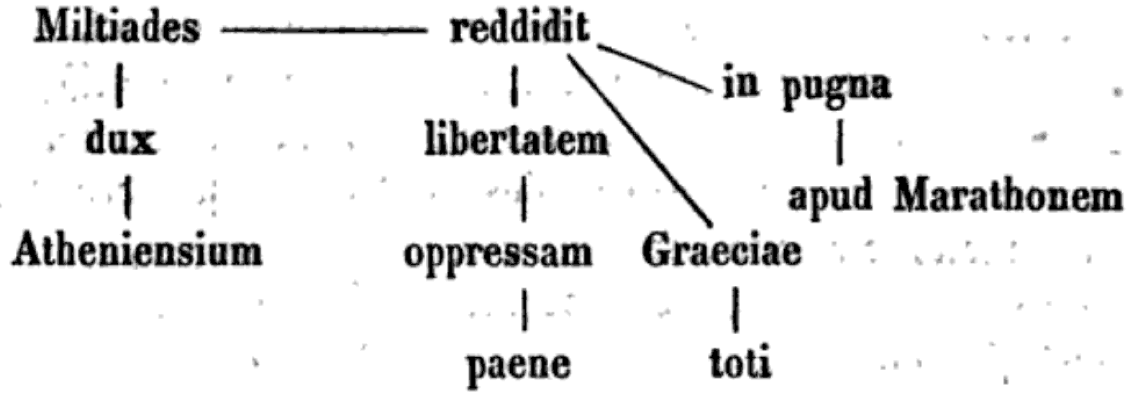
\includegraphics[width=\textwidth]{figures/vol1syntaxe2-img012.png}
    % \caption{\label{fig:}Diagramme de \citet{Billroth1832}}

    Stephen W. Clark est le premier grammairien à réellement exploiter des diagrammes dépendentiels dans sa grammaire de l’anglais de 1847 intitulé \textit{The science of the English grammar: A practical grammar in which words, phrases, and sentences are classified to their offices, and their relation to each other, illustrated by a complete system of diagrams} ‘La science de la grammaire anglaise : une grammaire pratique dans laquelle les mots, les syntagmes et les phrases sont classées selon leurs fonctions et leurs relations les uns aux autres par un système complet de diagrammes’. Dans les représentations de Clark, les connexions ne sont pas représentées en tant que telles : un mot qui en «~qualifie~» un autre (pour reprendre les termes de Clark) est placé dans une bulle sous la bulle de son gouverneur. Les prépositions comme \textit{by} ‘par’ ou \textit{of} ‘de’ dans la figure ci-dessous reçoivent une forme particulière indiquant qu’elles servent à «~connecter~» deux mots. Le sujet, le verbe et l’objet direct sont placés au même niveau, comme ici \textit{ressources} and \textit{are developed}. Les groupes prépositionnels sont entourés par des bulles en pointillés.

    % \caption{\label{fig:}Diagramme de \citet{Clark1847}}
    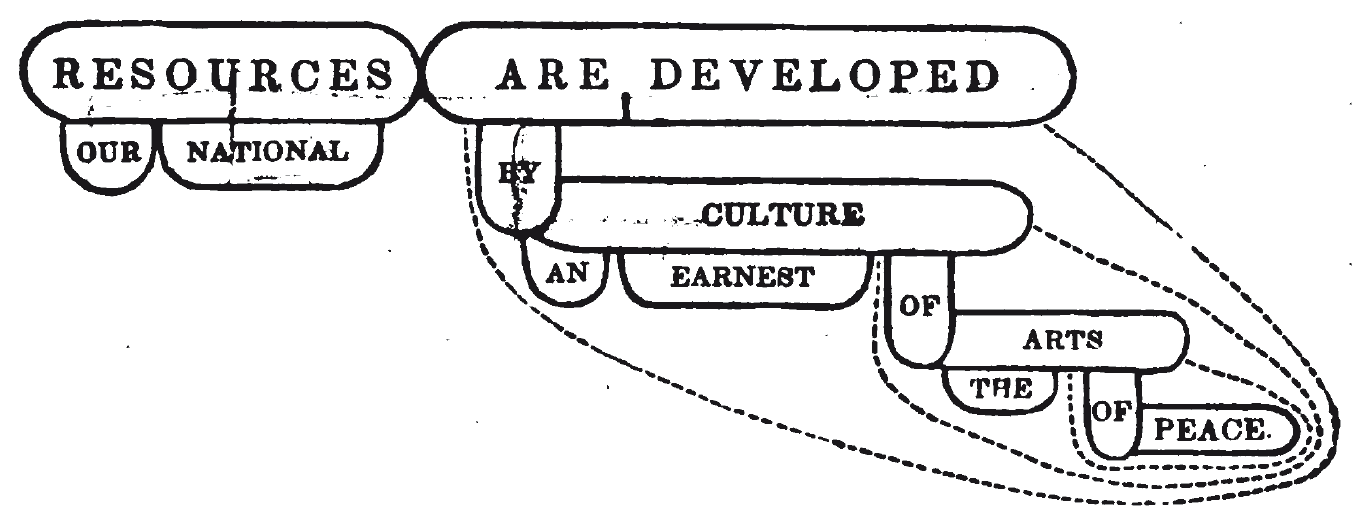
\includegraphics[width=\textwidth]{figures/vol1syntaxe2-img013.png}

    \textit{Our national resources are developed by an earnest culture of the arts of peace}\\
    ‘Nos ressources nationales sont développées grâce à une sérieuse culture des arts de la paix’

    Les analyses de Clark sont d’une grande cohérence et ses représentations de la coordination ou de l’extraction, sur lesquelles nous reviendrons dans les chapitres 5.3 et 5.4, sont remarquables. Il leur manque juste le développement théorique que proposera plus tard Tesnière.

    Ce ne sont pas les diagrammes de Clark qui sont passés à la postérité, mais ceux de ses suiveurs, \textbf{Alonzo Reed} and \textbf{Brainerd Kellogg}. Leurs diagrammes, proposés pour la première fois en 1877 et toujours utilisés aujourd’hui par certains enseignants d’anglais, sont équivalents à ceux de Clark, mais utilisent des conventions différentes : les mots ne sont plus placés dans des bulles, mais au-dessus de segments de traits. Les verbes et les noms reçoivent des segments horizontaux, comme \textit{pleased} ‘enchanté’ ou \textit{news} ‘nouvelles’ dans le diagramme qui suit, tandis que les autres mots, comme la préposition \textit{with} ‘avec’ ou l’adjectif ‘good’, reçoivent des segments en diagonal. Comme chez Clark, le sujet le verbe et l’objet sont au même niveau. Les connections apparaissent de manière plus explicite à la jointure de deux segments. La connexion entre le sujet et le verbe (\textit{girls – are pleased}) est symbolisée par un trait vertical et celle entre l’auxiliaire et le participe (\textit{are – pleased}) par un trait oblique.

    \ea
    %%[Warning: Draw object ignored]
    {The girls are pleased with the good news}\\
    ‘Les filles sont enchantées par la bonne nouvelle’

    Diagramme de \citet{ReedKellogg1877}
    \z

    On peut traduire cette structure dans les conventions utilisées ici, en réifiant les connexions et en mettant en évidence le fait que certaines connexions ne sont pas hiérarchisées :

    \ea
    %%[Warning: Draw object ignored]

    Interprétation du diagramme de Reed \& Kellogg
    \z

    En 1883, dans un livre sur la grammaire allemande (\textit{Zur Methodik des deutschen Unterrichts} ‘Sur la méthodologie de l’enseignement de l’allemand’), \textbf{Franz Kern} propose de véritables arbres de dépendance. Voici ce qu’il écrit : «~Le mot déterminant dépend de celui qu’il détermine ou, en d’autres termes, est régi par lui. On désigne (graphiquement, par un schéma) la dépendance d’un mot d’un autre par un trait partant du mot régissant vers le bas et allant vers le mot régi~(ou dépendant) [figure de gauche] ou encore sans mot par de simples relations grammaticales [figure de droite].~» Ce texte est accompagné des deux figures suivantes pour la phrase \textit{Eine alte Kirche wurde ausgebessert} ‘Une vielle église a été réparée’. Dans la figure de gauche figurent les mots de la phrase, le complexe verbal n’étant pas décomposé. Dans la figure de droite, l’article (appelé \textit{Adj. (Zeiger)} ‘adjectif (pointeur)’) et l’adjectif qualificatif (\textit{Adjektiv}) dépendent du mot sujet (\textit{Subjektswort}) qui dépend du verbe fini (\textit{Finites Verbum}).

    \ea
    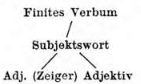
\includegraphics[width=.45\textwidth]{figures/vol1syntaxe2-img014.png}
    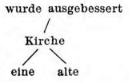
\includegraphics[width=.45\textwidth]{figures/vol1syntaxe2-img015.png}
    Arbres de dépendance de \citet{Kern1883}

    \textit{Eine alte Kirche wurde ausgebessert}\\
    ‘Une ancienne église a été reconstruite’
    \z

    La notion de \textit{valence} a été introduite par le sémioticien anglais Charles S. Peirce dans un article de 1897. Peirce compare la possibilité qu’a le verbe \textit{give} ‘donner’ de se combiner avec trois éléments (\textit{John gives John to John}) avec la possibilité qu’à l’atome d’azote N de se combiner avec trois atomes d’hydrogène H pour donner une molécule d’ammoniac NH\textsubscript{3}. Cette métaphore de la connexion entre mots par la connexion entre atomes est accompagnée de la figure suivante :

    \ea
    Schéma valenciel de \citet{Peirce1897}
    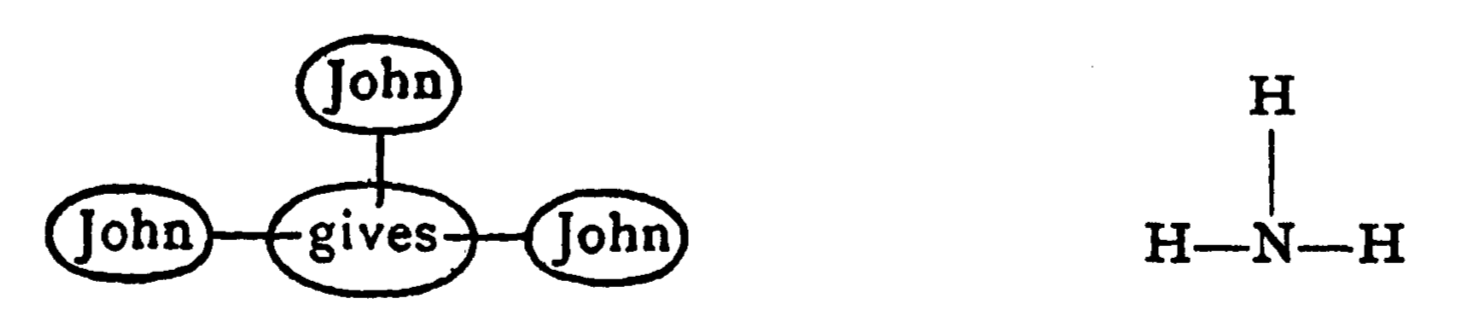
\includegraphics[width=\textwidth]{figures/vol1syntaxe2-img016.png}
    \z

    Peirce remarque que contrairement aux connections chimiques les connections entre mots (il s’agit plutôt de connexions sémantiques que syntaxiques) sont asymétriques, ce que semble confirmer son diagramme, où les connexions partent du mot \textit{gives} mais s’arrêtent à la bulle de \textit{John}. (Voir la \sectref{sec:3.3.10} sur \textit{Distribution et valence} pour la suite de la discussion.)

    C’est à Lucien Tesnière qu’on attribue les bases théoriques de la syntaxe de dépendance, exposées brièvement dans son article de 1934, \textit{Comment construire une syntaxe}, puis en détail dans son ouvrage posthume de 1959, \textit{Éléments de syntaxe structurale}. On notera, dans l’analyse suivante de 1934, que Tesnière considère la préposition comme dépendant du nom qu’elle introduit. (Le diagramme contient par ailleurs une erreur, qui n’est pas dans le manuscrit de Tesnière : le lien entre \textit{apporte} et \textit{vigueur} a été erronément attribué à \textit{elle}.)

    \ea
    Diagramme (tronqué) de \citet{Tesnière1934}
    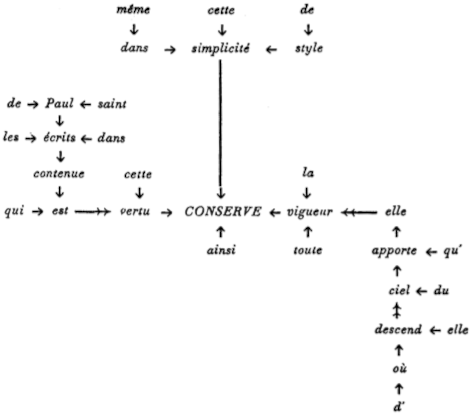
\includegraphics[width=\textwidth]{figures/vol1syntaxe2-img017.png}

    \textit{Ainsi cette vertu céleste, qui est contenue dans les écrits de saint Paul, même dans cette simplicité de style, conserve toute la vigueur qu’elle apporte du ciel d’où elle descend.} (Bossuet)
    \z

    Si cette analyse contient déjà des symboles spéciaux (comme les flèches à double pointe \textrm{$\twoheadrightarrow $} pour les relatives), ce n’est que plus tard que Tesnière introduira les symboles en T pour la translation. Les structures de l’ouvrage de 1959 ne sont plus totalement hiérarchique comme le montre notre interprétation polygraphique ci-dessous de la représentation proposée par Tesnière pour \textit{Écrivez dans le livre de votre ami} !.

    \ea

    %%[Warning: Draw object ignored]
    %%[Warning: Draw object ignored]
        Stemma de \citet{Tesnière1959}                 Interprétation polygraphique du stemma

    \z
}
\section{Arbre et représentation planaire}\label{sec:3.3.6}

Il est essentiel de rappeler que la \textbf{représentation par un arbre (de} \textbf{dépendance)} sert uniquement à encoder une \textbf{structure hiérarchique} liant des nœuds entre eux par des relations père-fils. Dès qu’un arbre est représenté sur une feuille plane, les nœuds frères (c’est-à-dire ayant le même père) doivent être placés les uns à côté des autres et apparaissent donc comme ordonnés. Cet ordre, imposé par la \textbf{représentation planaire}, est souvent utilisé pour ordonner implicitement des arbres (voir le \chapref{sec:3.5} où il sera justement question d’ordre linéaire et d’arbres ordonnés). Un arbre ordonné est néanmoins une structure plus riche qu’un simple arbre. Les arbres que nous considérons dans ce chapitre sont des \textbf{arbres non ordonnés}. Il faut se les imaginer dans l’espace, libérés de la feuille, comme des \textbf{mobiles} suspendus dans l’air et dont les nœuds peuvent tourner librement autour de leur gouverneur.

Pour en faciliter la lecture, nous placerons généralement les nœuds de nos arbres dans l’ordre qu’ils occupent dans la phrase, mais cet ordre n’a aucune pertinence lorsque l’arbre est considéré en tant que tel et nos lecteurs devront essayer d’en faire abstraction. Libérez les arbres de la feuille ! Faites-les tourner dans votre tête !

Nous allons maintenant voir comment définir l’arbre de dépendance. Pour cela nous allons introduire différents critères permettant d’identifier la tête d’une unité syntaxique.

\section{Critère d’effacement simple et critère prosodique}\label{sec:3.3.7}

Une première définition possible d’une structure de dépendance se base sur la structure de connexion. Lorsqu’on possède déjà une structure de connexion, on peut la hiérarchiser (au moins partiellement) simplement en choisissant un nœud racine dans la structure. On peut alors orienter les connexions en partant de la racine. Tout se passe comme si on attrapait la structure par ce nœud et qu’on la suspendait.

Illustrons cela avec la phrase :

\ea{
Pierre veut inviter Marie demain.
}
\z

Si l’on a la structure de connexion de cette phrase (voir \chapref{sec:3.2}) et qu’on peut établir que \textit{veut} est la tête (voir \sectref{sec:3.3.8} suivante), on obtient immédiatement une structure de dépendance par le procédé que nous venons de décrire. La flèche blanche indique le nœud par lequel on attrape la structure pour la hiérarchiser. Ce nœud va gouverner les nœuds auxquels il est connecté, lesquels vont gouverner à leur tour les nœuds auxquels ils sont connectés et ainsi de suite.

\begin{figure}
%%[Warning: Draw object ignored]

         \textbf{Structure de connexion}         \textbf{Arbre de dépendance}
\caption{\label{fig:}~}
\end{figure}

Si la structure de connexion n’a que des connexions élémentaires (voir l’\encadref{fig:3.2.23} \textit{Graphe à bulles et polygraphe}) et pas de cycles, on obtient un arbre de dépendance, comme dans l’exemple précédent.

Baser ainsi la dépendance sur la connexion, revient à donner une importance première aux propriétés définitoires des unités syntaxiques, l’\textstyleTermes{autonomisabilité illocutoire} et l’\textstyleTermes{autonomisabilité prosodique} (voir la \sectref{sec:3.2.11} \textit{Unité syntaxique autonomisable}). Traduit pour le repérage de la tête d’une unité, ces deux critères deviennent le critère d’effacement simple et le critère prosodique.

L’autonomisabilité illocutoire donne le critère suivant.

\begin{styleLivreImportant}
\textstyleTermes{Critère d’effacement simple} : si \textbf{l’unité} \textbf{AB est gouvernée par X} et que \textbf{B peut être effacé}, mais pas A, alors \textbf{A est la tête de AB} et B dépend de A.
\end{styleLivreImportant}

Dire que B peut être effacé et pas A lorsque AB est gouverné par X revient à dire que XA peut former une unité (illocutoirement) autonome, mais pas XB et donc que X est connecté à A. Comme X est le gouverneur de AB, on en déduit que A est la tête de AB.

Si on reprend notre exemple avec X = \textit{Pierre habite,} A = \textit{une maison} et B = \textit{écologique} et qu’on sait que X gouverne AB, alors on en déduit que B dépend de A, car B est effaçable (\textit{Pierre habite une maison}), mais pas A (*\textit{Pierre habite écologique}).

\begin{figure}
%%[Warning: Draw object ignored]

\caption{\label{fig:}Application du critère d’effacement simple}
\end{figure}

Attention : la présence d’un gouverneur est essentielle dans la formulation du  critère d’effacement simple. On trouve souvent la \textbf{mauvaise formulation} suivante : le dépendant d’une connexion est l’élément qui peut le plus facilement être effacé. Cette propriété n’est valable qu’en présence d’un gouverneur. Si AB est un énoncé autonome ou plus généralement si AB n’est pas gouverné on peut très bien effacer la tête de AB. Par exemple, dans \textit{Zoé chantait} (A = \textit{chantait}, B = \textit{Zoé}), on peut effacer A et pas B (\textit{Zoé} peut former un énoncé autonome, mais pas \textit{chantait}), alors que c’est A qui est la tête !

Passons maintenant à l’autonomisabilité prosodique, le deuxième critère qui nous a permis de définir la structure de connexion.

L’autonomisabilité prosodique donne le critère suivant.

\begin{styleLivreImportant}
\textstyleTermes{Critère prosodique~}: si X est le gouverneur de AB et si X \textbf{peut former une unité prosodique avec} A sans B (sans changer significativement le sens), alors A est \textbf{la tête de l’unité} AB.
\end{styleLivreImportant}

Les deux critères que nous venons de proposer sont insuffisants pour plusieurs raisons.

Premièrement, ils ne s’appliquent que dans le cas où l’on étudie une unité qui possède un gouverneur. Ils ne peuvent donc pas être utilisés pour déterminer la tête d’un énoncé. Ce point va être étudié dans la section suivante.

Deuxièmement, il est assez courant que deux éléments qui se combinent soient indissociables, à l’intérieur du mot bien sûr (\textit{chant-ons}), mais aussi en dehors, comme \textit{le chien} dans \textit{le chien dort}. Dans ce cas, le critère d’effacement simple ne s’applique pas, pas plus que le critère prosodique en général.

Troisièmement, le critère d’effacement simple est inopérant si B est un dépendant obligatoire de A. C’est le cas pour une combinaison comme \textit{à Marie}, où A = \textit{à} ne peut pas s’employer sans son complément B et ne peut donc jamais former une unité XA avec le gouverneur X de AB. C’est encore le cas pour les formes verbales finies de langues comme le français : en effet, pour \textit{Marie dormait}, il n’est pas possible de vérifier si A = \textit{dormait} peut former une unité avec un éventuel gouverneur X, puisque A ne s’emploie jamais sans un sujet B. Ceci a d’ailleurs amené Leonard Bloomfield (qui fut le premier, dans son ouvrage \textit{Langage} de 1933, à proposer des critères pour définir la tête) à considérer que ces constructions sont \textstyleTermes{exocentriques,} c’est-à-dire sans tête (voir la \sectref{sec:3.3.2} \textit{Historique des notions de dépendance et de tête}.)

Les limites du critère d’effacement simple et du critère prosodique nous amèneront à introduire d’autres critères plus puissants. Dans les critères que nous venons de considérer, le gouverneur X de l’unité AB que l’on étudie est fixé. On regarde seulement ce qui se passe dans une phrase donnée, sans faire varier X, A ou B. Cela confère à ces critères une grande simplicité d’utilisation, mais c’est aussi une limite. L’analyse distributionnelle va nous permettre de donner une version plus riche et plus fiable du critère d’effacement : le \textstyleTermes{critère distributionnel avec effacement}, présenté dans la \sectref{sec:3.3.11} éponyme.

\section{Tête d’un énoncé}\label{sec:3.3.8}

Comme nous l’avons vu à la section précédente, nous avons des critères pour identifier la tête d’une unité dès qu’on connaît son gouverneur, mais ces critères ne peuvent pas s’appliquer pour caractériser la tête d’un énoncé. Or, tant qu’on n’a pas identifié celle-ci et qu’on n’a pas un premier gouverneur, on ne peut pas appliquer le critère d’effacement simple ou le critère prosodique.

L’identification de la tête d’un énoncé repose sur les propriétés de l’énoncé en tant que tel, à savoir le fait qu’il fait l’objet d’une énonciation dirigée vers un interlocuteur et qu’il possède donc une \textstyleTermes{fonction illocutoire}. Cette notion repose sur le constat que produire un énoncé est une véritable action de la part du locuteur (on parle d’\textstyleTermes{actes de langage}, à la suite des travaux de \citet{Gardiner1932}, John \citet{Austin1962} et John \citet{Searle1969}), qui attend généralement en retour une action du ou des destinataire(s) (voir également la contribution de \citet{Bloomfield1933} dans la \sectref{sec:1.1.4} \textit{Sens et intention communicative}).

Ceci nous amène à considérer quatre types d’énoncés : \textstyleTermes{assertion}, \textstyleTermes{question}, \textstyleTermes{injonction} et \textstyleTermes{exclamation}.

\begin{itemize}
\item assertion : \textit{«~Il pleut.~»~}; \textit{«~J’ai mal au ventre.~»~};
\item question : «~\textit{Comment faire ?~»~}; «~\textit{Est-ce un problème ?~»} ;
\item injonction : «~\textit{Laissez ça ici !~»} ;
\item exclamation : «~\textit{Aie !~»~}; «~\textit{Comme c’est sympa !~».}
\end{itemize}

Les assertions peuvent être acceptés ou refusées par le destinataire ; elles se caractérisent par le fait de pouvoir être falsifiées par «~\textit{C’est faux.}~» ou au contraire validées par «~\textit{C’est vrai.}~». Par exemple, si quelqu’un nous dit «~\textit{J’ai mal au ventre}.~», on peut lui répondre «~\textit{C’est faux.}~», mais s’il dit «~\textit{Aie} !~», ce n’est plus possible. De même, on ne peut répondre «~\textit{C’est faux.}~» a une question ou une injonction. Les questions attentent une réponse. Les injonctions attendent généralement un acte non verbal. Les exclamations attendent simplement d’être partagées par le destinataire éventuel.

La fonction illocutoire a souvent un marquage spécifique. Les éléments qui servent à marquer la fonction illocutoire seront appelés des \textstyleTermes{marqueurs illocutoires}.

\begin{styleLivreImportant}
Nous faisons l’hypothèse que les \textbf{marqueurs illocutoires} sont \textbf{portés} par la \textstyleTermes{tête syntaxique de l’énoncé} et la caractérise.
\end{styleLivreImportant}

En français, le principal marqueur illocutoire est la prosodie (transcrit à l’écrit par des signes de ponctuation comme « ?~» ou « !~»). Mais pour les énoncés à tête verbale en français, il existe d’autres marques. Voyons sur un exemple :

\ea
{Pierre a dormi}.
\z

Cet énoncé est une assertion. Comme toute assertion, on peut la nier en répondant «~\textit{C’est faux}~».~La négation de cet énoncé (‘il est faux que Pierre a dormi’) peut s’exprimer en français par un double marquage \textit{ne…pas} qui semble bien identifier l’auxiliaire comme la tête :

\ea
{Pierre} \textbf{{n’a}  {pas}}  {dormi.}
\z

On peut également faire varier la fonction illocutoire et transformer cet énoncé en une question ou une injonction :
\ea
{Pierre} \textbf{{a-t-il}}  {dormi} ?
\z
\ea
\textbf{{Ais}}  {dormi (quand}  {je reviens)} !
\z

Le français a pour cela des formes particulières : une question peut prendre la \textstyleTermes{forme} dite \textstyleTermes{interrogative}, qui se caractérise par la présence d’un \textstyleTermes{enclitique} (\textit{{}-t-il} dans notre exemple) ; une injonction peut s’exprimer par une forme verbale particulière : l’\textstyleTermes{impératif} (ici \textit{ais}, forme impérative du verbe \textsc{avoir}). C’est encore une fois l’auxiliaire qui est touché, ce qui confirme son statut de tête.

On peut par la même méthode identifier la tête d’une phrase complexe avec deux verbes finis. Cette tête est traditionnellement appelée le \textstyleTermes{verbe principal}. Considérons :
\ea
{Marie pense que Pierre dort}.
\z
La forme interrogative est \textit{Marie pense-t-elle que Pierre dort} ? et pas *\textit{Marie pense que Pierre dort-il} ? On en déduit que \textit{pense} est la forme verbale principale et que \textit{dort} est une forme verbale subordonnée.

\begin{styleLivreImportant}
La \textstyleTermes{subordination} est simplement le terme traditionnel pour désigner la \textbf{dépendance d’une} \textbf{forme verbale} à un autre élément. Une unité syntaxique dont la tête est une forme verbale est appelée une \textstyleTermes{proposition}. Une proposition dont le verbe est subordonné est appelée une \textstyleTermes{proposition subordonnée}.
\end{styleLivreImportant}

L’identification de la subordination nous procure un nouveau test pour repérer la tête d’une proposition (voir \textbf{critère rectionnel} à la \sectref{sec:3.3.16} \textit{Tête interne et critère rectionnel}). En effet, certains verbes imposent un mode particulier à leur subordonné. Par exemple, si l’on subordonne au verbe \textsc{falloir} la proposition \textit{Pierre a dormi}, on obtient \textit{Il faut que Pierre} \textbf{\textit{ait}} \textit{dormi (quand je reviens).} Comme on le voit, encore une fois, c’est l’auxiliaire qui hérite ici de la marque de subordination, à savoir le \textstyleTermes{mode subjonctif} (\textit{ait} est une forme subjonctive de \textsc{avoir}), ce qui confirme son statut de tête syntaxique de la proposition.

On peut encore utiliser ces différents critères pour repérer que certains énoncés n’ont pas une tête verbale. Comparons les deux phrases suivantes :

\ea{
Heureusement, Pierre a dormi.
}
\z
\ea{
Heureusement que Pierre a dormi.
}
\z

On peut subordonner le premier énoncé, mais pas le deuxième :
\ea
{Je crois que, heureusement, Pierre a dormi}.
\z
\ea
*{Je crois qu’heureusement que Pierre a dormi}.
\z

Comme il apparaît par ailleurs que le verbe \textsc{croire} peut subordonner n’importe quelle proposition à l’indicatif, on peut supposer que la phrase introduite par \textit{heureusement que} ne peut pas être subordonnée car le verbe n’en est pas la tête. On en déduit que \textit{heureusement} est la tête de la phrase et subordonne la proposition \textit{Pierre a dormi} (ce que confirme l’emploi de la conjonction de subordination \textit{que}).

Le même type de raisonnement permet d’identifier la tête d’une proposition dans n’importe quelle langue a priori (voir encadré ci-dessous).

\globe{Tête d’un énoncé dans une langue inconnue}{%\label{sec:3.3.9}
    Comme nous l’avons dit dans les sections précédentes, l’identification de la tête d’un énoncé est un préalable à la hiérarchisation de la structure.

    Nous allons considérer le cas de deux langues non apparentées.
\begin{enumerate}
    \item Commençons par l’anglais, qui est une langue très proche du français, mais dont le fonctionnement est quand même différent. Considérons l’énoncé \textit{Peter has slept} ‘Pierre a (déjà) dormi’. Comme en français, la négation va sur l’auxiliaire sur lequel elle se cliticise :
    \ea
        {Peter} \textbf{{hasn’t}}  {slept.}  ‘Pierre n’a pas dormi.’
    \z
    Quant à la question, elle est normalement formée par l’antéposition de l’auxiliaire :
    \ea
        \textbf{{Has}}  {Peter slept?}    ‘Pierre a-t-il dormi ?’
    \z
    On peut considérer que cette place particulière de l’auxiliaire le marque comme la tête. D’ailleurs, un verbe ordinaire ne peut recevoir directement la négation, ni être antéposé. Le passage à une forme interrogative ou négative nécessite l’introduction de l’auxiliaire \textsc{do} ‘faire’ :
    \ea
        {Peter slept.}    ‘Pierre a dormi.’
    \z
    \ea
        \textbf{{Did}}  {Peter sleep?}    ‘Pierre a-t-il dormi ?’
    \z
    \ea
        {Peter} \textbf{{didn’t}}  {sleep.}  ‘Pierre n’a pas dormi.’
    \z
    Comme on le voit, la forme passé \textit{slept} passe à la forme infinitive. L’auxiliaire lui-même hérite de la finitude (\textit{did} est la forme passé de \textsc{do}) et constitue donc la tête de la phrase quand il est présent. En l’absence d’auxiliaire, c’est la forme verbale simple qui est la tête, puisque c’est elle qui est affectée lorsque l’auxiliaire est introduit. On notera que l’auxiliaire, bien qu’il soit la tête de la phrase, peut dans certains cas se cliticiser sur le sujet (c’est-à-dire perdre la possibilité de recevoir un accent tonique et former un mot prosodique avec le dernier mot du sujet) :
    \ea
        {Peter}\textbf{{’s}}  {sleeping} =  {Peter} \textbf{{is}}  {sleeping}  ‘Pierre est en train de dormir’, lit. Pierre est dormant.
    \z
    \ea
        {Peter}\textbf{{’s}}  {eaten}   =   {Peter} \textbf{{has}}  {eaten}   ‘Pierre a (déjà) mangé’
    \z
    \item En coréen, le verbe principal d’un énoncé est caractérisé par un marqueur de politesse qu’il est le seul à pouvoir porter. Cette particule s’ajoute optionnellement sur le verbe principal, mais jamais sur un verbe subordonné. Le coréen utilise essentiellement des constructions à verbe support (voir \chapref{sec:2.4}) avec le verbe \textsc{hada} ‘faire’. Dans la phrase suivante, le sens ‘aimer’ est ainsi lexicalisé par le nom \textsc{sarang} ‘amour’ et le sens ‘croire’ par le nom \textsc{saenggak} ‘pensée’, tous deux «~verbalisés~» par le verbe \textsc{hada}. La deuxième occurrence de \textsc{hada} peut porter le morphème de politesse \textit{yo}, mais pas la première. (Nous reviendrons sur les marqueurs illocutoires du coréen dans l’\encadref{fig:5.1.12} \textit{Des prédicatifs uniquement locutifs assertifs}.)

    \ea
    \ea[]{
    \gll   Ch’ŏlsu-ga na-rŭl sarang-ha-ndago saenggak-hae(-\textbf{yo})\\
    Ch’ŏlsu-\textsc{nom}   moi-\textsc{acc}  amour-faire-\textsc{pres.inf}  pensée-faire(-\textsc{politesse)}\\}
    \glt   ‘Je crois que Cholsu m’aime’
    \ex[*]{
    \gll   Ch’ŏlsu-ga            na-rŭl            sarang-hae-\textbf{yo}-ndago  saenggak-hae(-\textbf{yo})\\
        Ch’ŏlsu-\textsc{nom}  moi-\textsc{acc}  amour-faire-\textsc{pres.inf}  pensée-faire(-\textsc{politesse)}\\}
    \z
    \z
    \end{enumerate}
}
\section{Distribution et valence}\label{sec:3.3.10}

En nous basant sur la structure de connexion et en déterminant la tête de la proposition grâce aux marqueurs illocutoires, nous avons vu que nous pouvions obtenir une structure de dépendance partielle. Nous allons voir que l’on peut raffiner cette structure en ajoutant des critères additionnels. Les premiers de ces critères sont les critères distributionnels que nous présenterons dans les sections suivantes. Nous devons avant cela introduire les notions de distribution (voir la \sectref{sec:2.1.7} sur \textit{L’identification des unités de la langue}, où il a été question d’analyse distributionnelle) et valence (voir la \sectref{sec:3.3.5} \textit{Historique des représentations syntaxiques par des diagrammes en dépendance} pour un début de discussion).

\begin{styleLivreImportant}
La \textstyleTermes{distribution} d’une unité est l’\textbf{ensemble des contextes} ou \textbf{environnements} où peut se trouver cette unité.
\end{styleLivreImportant}

Deux remarques essentielles sont à faire concernant la distribution.

Premièrement, nous faisons de l’analyse distributionnelle sur un objet structuré. Ici, ce qui nous intéresse, c’est la \textstyleTermes{distribution syntaxique} et non la distribution linéaire. Nous nous intéressons donc au contexte des unités au sein de la structure syntaxique, c’est-à-dire au \textstyleTermes{paradigme} des unités qui se combinent avec l’unité que nous étudions.

La notion de distribution est encore exprimable en termes de valence.

\begin{styleLivreImportant}
La \textstyleTermes{valence} d’une unité syntaxique est la \textbf{capacité} qu’à cette unité \textbf{à se combiner} avec d’autres unités syntaxiques. La valence est avant tout une \textbf{valence potentielle}, à contraster avec la \textbf{valence réalisée}, lorsque l’unité est utilisée dans un contexte donné.
\end{styleLivreImportant}

Cette métaphore de la valence est inspirée de la chimie et de la capacité qu’à un atome à \textbf{se combiner avec d’autres} \textbf{atomes pour former des molécules} (voir la contribution de \citet{Peirce1897} dans l’\encadref{fig:3.3.5} \textit{Historique des représentations syntaxiques par des diagrammes en dépendance}, ainsi que les formules utilisées par \citet{Jespersen1937}, évoquées dans l’\encadref{fig:3.3.2} \textit{Historique des notions de dépendance et de tête}). Mais alors que les connexions entre atomes sont symétriques (chaque atome fournit un électron de même nature), les connexions entre unités sont doublement asymétriques : \textbf{asymétrie syntaxique}, puisqu’elles lient un gouverneur à un dépendant, et \textbf{asymétrie sémantique}, puisqu’elle lient un prédicat à un argument.

L’asymétrie syntaxique nous amène à distinguer deux parties dans la valence.

\begin{styleLivreImportant}
La \textstyleTermes{valence supérieure} d’une unité syntaxique U est la \textbf{position syntaxique} occupée par le \textbf{gouverneur} de U, cette position étant elle-même caractérisée par le \textbf{paradigme} des éléments qui peuvent l’occuper.
\end{styleLivreImportant}

\begin{styleLivreImportant}
A l’inverse, la \textstyleTermes{valence inférieure} d’une unité syntaxique est l’ensemble des positions syntaxiques qui \textbf{dépendent} potentiellement de cette unité.
\end{styleLivreImportant}

Les notions de valences supérieure et inférieure ont été introduites par Igor Mel’čuk, qui les nomment \textit{valence passive} et \textit{valence active}. Nous préférons garder ces termes pour parler de la partition de la valence selon le point de vue sémantique.

Deuxièmement, nous souhaitons utiliser l’analyse distributionnelle pour caractériser la tête d’une unité. Nous cherchons donc à repérer dans le contexte syntaxique d’une unité le contexte qui caractérise plus particulièrement la tête, c’est-à-dire la valence supérieure.

Illustrons ce dernier point par un exemple. Considérons l’énoncé \textit{Une très vieille dame habite ici} et l’unité syntaxique \textit{vieille dame} qu’il contient. Aucun des deux mots \textit{vieille} et \textit{dame} ne contrôlent à lui seul l’entièreté de la distribution de l’unité qu’ils forment ensemble, car \textit{vieille} est connecté à \textit{très} (\textit{très vieille}) et \textit{dame} est connecté à \textit{une} et \textit{habite} (\textit{une dame habite ici}). Bien sûr, une fois que l’on sait que \textit{habite} est la tête de la phrase, on en déduit que la tête de \textit{vielle dame} est \textit{dame}, puisque c’est le mot qui est connecté au gouverneur de cette unité syntaxique.

On ne dira jamais assez qu’on ne peut \textbf{déterminer la tête} d’une unité syntaxique U par la distribution qu’\textbf{une fois qu’on} \textbf{a déterminé la valence supérieure} de U, c’est-à-dire qu’on a déterminé qui parmi les éléments auxquels U est connectée gouverne U. Considérer la distribution sans avoir au préalable distingué valence inférieure et supérieure peut conduire à des erreurs méthodologiques. Il y a là un cercle vicieux dans lequel il faut éviter de rentrer, puisqu’on ne peut appliquer de critère distributionnel pour déterminer la tête d’une unité sans savoir où se trouve son gouverneur. Autrement dit, il s’agit d’un critère pour déterminer la hiérarchie qui ne peut s’appliquer sans connaître déjà une partie de la hiérarchie.

Supposons que l’on veuille déterminer qui du nom ou du déterminant est la tête du groupe qu’ils forment ensemble (comme par exemple \textit{chat} et \textit{le} dans \textit{le chat dort}). Si l’on décrète que pouvoir être sujet d’un verbe fait partie de la valence supérieure du nom, le problème est biaisé, puisque, en un sens, on a déjà décidé que le nom est la tête du groupe qu’il forme avec le déterminant (on trouve cette erreur dans l’ouvrage de référence d’Igor Mel’čuk de 1988). Tout le problème ici est qu’on ne peut facilement déterminer la valence supérieure du nom seul, car, dans de nombreuses positions, il est indissociable d’un déterminant. (Voir la \sectref{sec:3.3.23} sur \textit{Nom ou déterminant comme tête} ?) Nous avons contourné ce problème en définissant au préalable la structure de connexion (\chapref{sec:3.2}), puis en hiérarchisant sommairement cette structure en déterminant la tête d’un énoncé (\sectref{sec:3.3.8}), ce qui nous permet de localiser la valence supérieure d’un certain nombre d’unités (mais pas des noms malheureusement !).

\section{Le critère distributionnel avec effacement}\label{sec:3.3.11}

Les critères distributionnels s’appliquent à une unité syntaxique U dont on connaît la \textbf{valence supérieure}, c’est-à-dire le \textbf{paradigme des gouverneurs possibles} (voir \sectref{sec:3.3.10}).

\begin{styleLivreImportant}
Une \textstyleTermes{tête distributionnelle} de U est un élément qui contrôle la valence supérieure de U. Autrement dit, si B dépend de A, alors B ne modifie pas la valence supérieure de A.
\end{styleLivreImportant}

Nous allons voir deux critères distributionnels. Le premier, le critère distributionnel avec effacement suppose que A et B ne sont pas mutuellement indissociables pour être appliqué.

\begin{styleLivreImportant}
\textstyleTermes{Critère distributionnel avec effacement~}: Si A est autonomisable (et donc B est effaçable) et que A a la \textbf{même valence supérieure} que U = A ${\oplus}$ B alors A est une \textbf{tête distributionnelle} de U. Inversement, si A est autonomisable (et B est effaçable), mais que A n’a \textbf{pas} la même valence supérieure que U = A ${\oplus}$ B, alors B est une \textbf{tête distributionnelle} de U.
\end{styleLivreImportant}

Ce critère généralise le critère d’effacement simple. Le critère d’effacement simple s’applique à une unité U à l’intérieur d’un énoncé donné, sans faire varier le gouverneur de U. Ici on considère la distribution de U, c’est-à-dire tous les gouverneurs potentiels de U.

Illustrons le critère par l’exemple de U = \textit{une maison écologique} avec A = \textit{une maison} et B~= \textit{écologique}. Ici A et B sont effaçables et on peut donc comparer la valence supérieure de A, B et U = A ${\oplus}$ B. Il est facile de voir que \textit{une maison} et \textit{une maison écologique} ont la même valence supérieure (ils peuvent par exemple tous les deux être sujet ou objet d’un verbe ou se combiner avec une préposition) et qu’elle est différente de la valence supérieure de \textit{écologique} qui ne peut apparaître dans aucun de ces contextes. On en déduit que \textit{une maison} est la tête de U.

Le critère distributionnel avec effacement s’applique dans des cas où le critère d’effacement simple ne s’applique pas. Reprenons l’exemple de U = \textit{à Marie}. Ici \textit{Marie} n’est pas effaçable, puisque \textit{à} n’est pas autonomisable. Par contre, \textit{à} est effaçable, on peut donc comparer les valences passives de \textit{Marie} et \textit{à Marie}. Ces deux unités ont des valences passives complètement différentes. Par exemple, \textit{Marie} peut être sujet (\textit{Marie dort}) ou complément d’objet (\textit{J’ai vu Marie}) et la commutation avec \textit{à Marie} est impossible (*\textit{A Marie dort} ; *\textit{J’ai vu à Marie}). On en déduit que \textit{à} est la tête de \textit{à Marie}.

Le même raisonnement est applicable à \textit{Marie dormait}. Ici encore, \textit{Marie} n’est pas effaçable, mais \textit{dormait} l’est. Comme \textit{Marie} et \textit{Marie dormait} n’ont absolument pas la même valence supérieure, on en déduit \textit{dormait} est bien la tête de la proposition \textit{Marie dormait}.

\loupe{Tête effaçable}{%\label{sec:3.3.12}
    Il arrive quelquefois que le critère d’effacement simple et le critère distributionnel avec effacement se contredisent. On parle alors de \textstyleTermesapprofondissement{tête effaçable}. L’exemple le plus clair est celui de la conjonction de subordination \textit{that} en anglais. Voyons un exemple :
    \ea
        {Mary thinks that Peter slept.}  ‘Mary pense que Pierre dormait.’
    \z
    \ea
        {Mary thinks Peter slept.}    ‘Mary pense que Pierre dormait.’
    \z
    La conjonction \textit{that} est bien effaçable, ce qui pourrait conduire à considérer que \textit{thinks} est directement connecté à \textit{slept}. Mais en même temps on ne peut pas considérer que \textit{that} dépend de \textit{slept} car \textit{that Peter slept} n’a pas la même valence supérieure que \textit{Peter slept} : si les deux peuvent dépendre de \textit{Mary thinks}, seul \textit{Peter slept} peut former un énoncé déclaratif ou bien se combiner avec une conjonction comme \textit{if} ‘sis’ ou \textit{whether} ‘si (oui ou non)’. Comme un dépendant ne peut modifier la valence supérieure de son gouverneur, il est donc clair que \textit{that} n’est pas un dépendant du verbe \textit{slept}. (Voir l’\encadref{fig:3.3.28} sur la \textit{Co-occupation} pour une autre analyse de \textit{that}.)

    \ea
    %%[Warning: Draw object ignored]

            \textbf{Structure de connexion}    \textbf{Arbre de dépendance}
    \z
    De tels cas sont rares et le critère d’effacement simple reste un critère simple généralement fiable.
}
\section{Le critère distributionnel sans effacement}\label{sec:3.3.13}

Le critère distributionnel avec effacement n’est applicable à une unité U = A ${\oplus}$ B que si A ou B est effaçable. Il ne peut donc être appliqué pour des unités dont les composantes sont mutuellement indissociables comme le radical et sa flexion dans U = \textit{chant-ons}. On peut utiliser alors un autre critère distributionnel, applicable dans tous les cas.

\begin{styleLivreImportant}
\textstyleTermes{Critère distributionnel sans effacement} : C’est seulement si A est une \textbf{tête distributionnelle} de U que la commutation de A avec A’ peut donner une nouvelle unité U’ dont la \textbf{valence supérieure} est \textbf{différente} de celle de U. Autrement dit, si U = A ${\oplus}$ B, A commute avec A’ et U’ = A’ ${\oplus}$ B a une valence supérieure différente de A, alors A est une tête distributionnelle de U.
\end{styleLivreImportant}

(Voir l’exercice 4, \sectref{sec:3.3.35}, et sa correction, \sectref{sec:3.3.37}, pour une autre formulation du critère due à Paul Garde, 1977 : 8.) Si l’on applique ce critère à une unité U = A ${\oplus}$ B dont on veut déterminer la tête, on considèrera le paradigme des éléments A’ qui commutent avec A et le paradigme des éléments B’ qui commute avec B et on comparera les valences supérieures de U~= A ${\oplus}$ B, U’ = A’ ${\oplus}$ B et U” = A ${\oplus}$ B’, c’est-à-dire le paradigme des unités X qui peuvent gouverner ces différentes unités.

\begin{figure}
%%[Warning: Draw object ignored]

\caption{\label{fig:}Application du critère distributionnel sans effacement}

\end{figure}

On regardera ainsi laquelle des deux commutations, celle sur A ou celle sur B, a le plus d’impact sur la valence supérieure de U. Si les A ${\oplus}$ B’ ont la même valence supérieure que A ${\oplus}$ B, mais pas les A’ ${\oplus}$ B, on en déduira que A gouverne B, c’est-à-dire que A est la tête de la combinaison U = A ${\oplus}$ B.

Montrons par un exemple comment s’applique le critère. Considérons U = \textit{chantons} qui est la combinaison du lexème A = \textsc{chanter} de signifiant \textit{chant-} et de la flexion verbale B = \textit{{}-ons} = indicatif ${\oplus}$ présent ${\oplus}$ 1\textsuperscript{re} personne ${\oplus}$ pluriel (voir le \chapref{sec:4.2} sur les \textit{Catégories flexionnels} pour les détails de cette décomposition et la discussion sur la présence de syntaxèmes zéros). On peut faire commuter A avec les autres lexèmes verbaux et B avec les autres flexions verbales. Quel que soit le lexème verbal A’ considéré, l’unité U’ =  A’ ${\oplus}$ B garde la même valence supérieure que U, celle d’une proposition à l’indicatif, qui peut être aussi bien une phrase complète qu’une proposition subordonnée à un verbe qui impose l’indicatif (\textit{Je sais que nous chantons}). Par contre, ni U, ni U’ ne pourra être subordonnée à un verbe qui demande le subjonctif (\textit{*Je veux que nous chantons} vs \textit{Je veux que nous chantions}). Autrement dit, la commutation de B avec un subjonctif changera la valence supérieure de U. Même le changement du présent en futur change la valence supérieure, puisqu’il existe des contextes où le futur est impossible (\textit{Si nous chantons, les gens vont partir} vs *\textit{Si nous chanterons, les gens vont partir}). La commutation de B avec un infinitif (\textit{chanter}) ou avec un participe (\textit{chanté} ou \textit{chantant}) modifie encore davantage la valence supérieure de la forme verbale. Nous en concluons que, sans aucun doute possible, c’est la flexion du verbe et non le verbe lui-même qui contrôle la valence supérieure d’une forme verbale.

Le critère distributionnel sans effacement peut également s’appliquer quand le critère distributionnel avec effacement s’applique. Le critère sans effacement est néanmoins moins simple à utiliser que celui avec effacement. En effet, pour ce dernier, il n’y a que trois unités à tester (U = A ${\oplus}$ B, A et B) et non toutes les unités obtenues en faisant varier A ou B. On peut considérer le critère distributionnel avec effacement comme un cas limite du critère distributionnel sans effacement, une commutation par le vide.

\section{ Tête faible}\label{sec:3.3.14}

Reprenons l’exemple de U = \textit{à Marie,} avec A = \textit{à} et B = \textit{Marie}. Le critère distributionnel avec effacement (\sectref{sec:3.3.11}) nous a permis de déterminer que A = \textit{à} est une tête distributionnelle. Voyons maintenant ce que nous dit le critère distributionnel sans effacement sur les propriétés de tête de A et B. Le syntagme U peut dépendre de \textsc{téléphoner} (\textit{Pierre téléphone à Marie}), mais si on commute A = \textit{à} avec une autre préposition (\textit{de Marie}, \textit{sur Marie}), le syntagme peut continuer à dépendre d’un verbe (\textit{Pierre rêve de Marie, Pierre compte sur Marie}), mais pas du verbe \textsc{téléphoner}. On en déduit à nouveau que la préposition \textit{à} est une tête distributionnelle et qu’elle ne dépend donc pas du substantif B. (Pour l’utilisation du terme \textit{substantif}, voir la \sectref{sec:3.3.23} \textit{Nom ou déterminant comme tête} ?.) Avant d’en conclure que le substantif B dépend de la préposition A, il faut regarder ce qui se passe quand on commute le substantif B.

Le substantif B = \textit{Marie} peut commuter avec beaucoup de groupes substantivaux sans que cela n’affecte la valence supérieure du groupe (\textit{Pierre téléphone à}\textbf{ \textbf{une} \textit{amie/à} \textit{tout le monde/aux} \textit{autres/…}}), mais B peut difficilement commuter avec un inanimé (\textit{Pierre téléphone à} \textbf{\textit{quelqu’un}};~\textsuperscript{?*}\textit{Pierre téléphone à} \textbf{\textit{quelque chose}}). De plus, B peut commuter avec un infinitif, mais pas dans ce contexte (\textit{Pierre commence} \textbf{\textit{à partir}} vs *\textit{Pierre téléphone à} \textbf{\textit{partir}}). On en déduit que la préposition \textit{à} est plutôt la tête distributionnelle, mais que le substantif contrôle quand même une partie de la distribution.

\begin{styleLivreImportant}
Lorsqu’un deuxième élément contrôle également la distribution de l’unité U, la tête de U est dite \textstyleTermes{faible}.
\end{styleLivreImportant}

Le groupe prépositionnel est donc une unité à tête faible. Ceci nous permet de postuler la structure de dépendance ci-dessous (figure de gauche). Mais on peut aussi vouloir privilégier le rôle de tête de la préposition et obtenir un arbre de dépendance (figure de droite).

\begin{figure}
%%[Warning: Draw object ignored]
%%[Warning: Draw object ignored]

    \textbf{Structure de dépendance}      \textbf{Arbre de dépendance}
        avec tête faible
    \caption{\label{fig:}}
\end{figure}

Notons qu’il existe une solution plus «~lexicale~» au fait que la préposition \textit{à} puisse avoir aussi bien un complément substantif (\textit{à Marie}) qu’infinitif (\textit{à arriver}). La solution consiste à considérer que la préposition \textit{à} a deux entrées lexicales différentes, l’une dont le complément est un substantif et l’autre un infinitif. Dans ce cas, on considère que les verbes \textsc{teléphoner} (\textit{téléphoner à Marie}) et \textsc{commencer} (\textit{commencer à arriver}) régissent des prépositions \textit{à} différentes et il n’est plus nécessaire de dire que le complément de la préposition contrôle la valence supérieure du groupe prépositionnel.



\maths{Quelle structure pour quels critères ?}{%\label{sec:3.3.15}
    En définissant la structure de connexion à partir de critères caractérisant les unités autonomisables (illocutoirement et/ou prosodiquement), nous obtenons une structure qui encode ces mêmes unités (voir la \sectref{sec:3.2.19} \textit{Structure de connexion et unités}). Par contre, si l’on ajoute des critères pour raffiner la structure celle-ci n’encode plus les unités autonomisables, comme nous l’avons déjà mentionné dans l’\encadref{fig:3.2.20} sur \textit{Les limites de la dualité}. C’est ce qui se passe avec les critères introduits dans ce chapitre qui nous ont permis d’obtenir une structure de dépendance plus fine que la structure de connexion. On peut néanmoins récupérer l’information sur les unités autonomisables en indiquant quelles dépendances ne peuvent être coupées, c’est-à-dire en indiquant pour chaque dépendant s’il est optionnel ou obligatoire.

    On peut maintenant se demander quel est l’intérêt d’introduire de nouveaux critères et de raffiner ainsi la structure. Il ne faut pas perdre de vue les objectifs qui prévalent à la définition d’une structure syntaxique. L’un des principaux objectifs de la structure syntaxique est de servir de support à l’écriture des règles de la grammaire. Nous devons donc privilégier la structure qui permet d’exprimer le plus simplement possible les principales contraintes qui pèsent sur la formation des énoncés. C’est pour cela que nous souhaitons que les éléments qui se contraignent les uns les autres soient liés dans la structure. Ceci nous permettra d’assurer les \textbf{contraintes distributionnelles} par des \textstyleTermesapprof{règles locales}, c’est-à-dire des règles qui s’appliquent à une portion bien circonscrite de la structure.

    Ajoutons encore que la structure que nous associons à un énoncé représente seulement les propriétés de notre énoncé vis-à-vis des critères appliqués. Nous aimerions que la structure que nous obtenons ait une réalité cognitive, qu’elle soit construite par le locuteur lorsqu’il produit ou comprend un énoncé, mais nous n’avons pas vraiment les moyens de le montrer (voir néanmoins notre tentative dans le \chapref{sec:1.2} \textit{Produire un énoncé}).
}
\section{Tête interne et critère rectionnel}\label{sec:3.3.16}

La \textbf{tête distributionnelle} est aussi appelée la \textstyleTermes{tête externe}, parce que c’est l’élément qui est «~visible~» de l’extérieur d’une unité syntaxique. On peut opposer aux critères externes de l’effacement et de la distribution, des critères internes, que nous appellerons les \textstyleTermes{critères de rection}. Ceux-ci s’appliquent à la combinaison de deux éléments, indépendamment des contextes où peut être placée l’unité formée par leur combinaison et donc sans regard pour ce qui se passe à l’extérieur de cette combinaison.

\begin{styleLivreImportant}
On appelle \textstyleTermes{tête interne} d’une combinaison l’élément qui semble imposer à l’autre sa forme, sa catégorie ou sa position linéaire. La tête interne est encore appelée le \textstyleTermes{régissant} et l’élément qui dépend de lui est dit \textstyleTermes{régi}.
\end{styleLivreImportant}

Par exemple, le verbe \textsc{téléphoner} impose à son complément d’être combiné avec la proposition À (\textit{Pierre téléphone à Marie}) tandis que le verbe \textsc{regarder} demande un complément nu (\textit{Pierre regarde Marie}).

\begin{styleLivreImportant}
La contrainte que le régissant impose au régi et son expression (par un syntaxème de cas, une préposition ou une place linéaire par exemple) est appelée le \textstyleTermes{régime}. À noter que l’on parle aussi bien du \textbf{régime du régissant}, pour désigner l’ensemble des contraintes qu’il impose à ses dépendants, que du \textbf{régime du régi}, pour désigner la forme particulière que lui impose son gouverneur.
\end{styleLivreImportant}

Une préposition imposée par un régime, comme la préposition À imposée par le verbe \textsc{téléphoner} à son complément, est appelée une \textstyleTermes{préposition régime}.

Le critère rectionnel permet par exemple de confirmer que l’auxiliaire est bien la tête d’une forme verbale complexe. Comparons :

\ea
{Pierre a dorm}\textbf{{i}}  {longtemps.}
\z
\ea
{Pierre va dorm}\textbf{{ir}}  {longtemps.}
\z

On voit que l’auxiliaire du passé impose au verbe lexical d’être au participe passé, tandis que l’auxiliaire du futur impose au verbe d’être à l’infinitif. On en déduit que l’auxiliaire régit le verbe auxilié.

Une formulation inverse du critère rectionnel est le \textstyleTermes{critère d’indépendance des codépendants}. On appelle \textstyleTermes{codépendants} deux éléments qui dépendent du même regissant.~

\begin{styleLivreImportant}
Un élément n’impose pas à un codépendant sa forme, sa catégorie ou sa position linéaire.
\end{styleLivreImportant}

Un élément peut toutefois occuper la place habituellement dévolue à un de ses codépendant, mais il ne contrôle pas la place où celui-ci est déplacé.

Donnons l’exemple du wolof. Le verbe en wolof est quasiment invariable, mais il peut se combiner avec un certain nombre de particules verbales. La question est alors : ces particules doivent-elles être traitées comme des adverbes modifiant le verbe ou comme des auxiliaires régissant le verbe ? Ces particules verbales modifient la distribution du verbe (par exemple, les particules ne sont pas possibles dans les constructions relatives), ce qui en fait donc des têtes distributionnelles. Mais elles ont une autre propriété qui en fait aussi des têtes internes. En effet, chaque particule promeut un élément différent en première position : la particule \textit{a} maintient le sujet en première position, la particule \textit{la} promeut un complément, la particule \textit{na} promeut le verbe lui-même et enfin la particule \textit{da} occupe la première position.

\ea
\gll  {ñu=}\textbf{{a}}{=y}                {lekk}          {am}       {xar~}\\
\textsc{S3pl=part=imp} manger  \textsc{indef}  mouton\\
\glt `C’est eux qui mangent un mouton.’
\z

\ea
\gll  {am}       {xar~}          \textbf{{la}}\textit{=ñu=y}               {lekk}\\
\textsc{indef}  mouton  \textsc{part=S3pl=imp} manger\\
\glt `C’est un mouton qu’ils mangent.’
\z

\ea
\gll  {lekk}       \textbf{{na}}\textit{=ñu=y}             {am}       {xar~}\\
manger  \textsc{part=S3pl=imp} \textsc{iààndef}  mouton\\
\glt `Ils mangent un mouton.’
\z

\ea
\gll \textbf{{da}}{{}-ñu=y              lekk         am      xar~}\\
\textsc{part=S3pl=imp} manger  \textsc{indef}  mouton\\
\glt `(Le fait est que) ils mangent un mouton.’
\z

En plus, la particule \textit{la} autorise la réalisation d’un sujet lexical post-verbal, tandis que les particules \textit{na} et \textit{da} l’interdisent. Ces propriétés montrent que les particules ne peuvent pas être dépendantes du verbe, en raison du critère d’indépendance des codépendants : un dépendant du verbe ne peut imposer sa place à un autre dépendant du verbe comme le font les particules verbales.

Notons pour terminer que lorsque les critères pour identifier la tête interne et la tête externe se contredisent, ce sont les critères distributionnels (avec et sans effacement) et la tête externe que nous privilégions.

\section{Critère de la tête sémantique}\label{sec:3.3.17}

La tête syntaxique d’une unité syntaxique n’est en général pas seulement saillante du point de vue distributionnel : elle est aussi saillante du point de vue sémantique et constitue alors ce qu’on appelle la tête sémantique de l’unité.

\begin{styleLivreImportant}
La \textstyleTermes{tête sémantique} d’une unité U est l’élément de U qui résume à lui seul le sens de U, qui en détermine la catégorie ontologique.
\end{styleLivreImportant}

Par exemple, la tête sémantique de \textit{poisson-chat} est \textit{poisson}, car un poisson-chat est un type de poisson et pas un type de chat. À l’inverse, \textit{enseignant-chercheur} apparaît comme exocentrique, car un enseignant-chercheur est autant un enseignant qu’un chercheur. (Voir l’\encadref{fig:3.1.12} \textit{Constructions N+N} \textit{ou N}${\oplus}$\textit{N} ?.)

La tête sémantique d’une proposition est le verbe. Ainsi la proposition \textit{Zoé invite ses copains à son anniversaire} décrit-elle avant tout une invitation dont Zoé, ses copains ou l’anniversaire sont des participants.

La tête sémantique d’une unité syntaxique n’est pas toujours sa tête syntaxique : la notion de tête sémantique privilégie les sémantèmes lexicaux vis-à-vis des éléments grammaticaux. Ainsi la tête sémantique de \textit{Zoé a invité ses copains à son anniversaire} reste le verbe lexical \textsc{inviter} et n’est pas l’auxiliaire \textsc{avoir} qui marque le passé. De la même façon, la tête sémantique d’un groupe substantival comme \textit{le chien de Marie} privilégie le nom tête \textsc{chien} au détriment du déterminant \textsc{le}.

La notion de tête sémantique est donc une notion distincte de celle de tête syntaxique (voir l’\encadref{fig:3.3.19} sur les \textit{Distorsions sémantique-syntaxe}). Néanmoins lorsque les critères pour déterminer la tête syntaxique sont insuffisants, on peut, si l’on souhaite à tout prix choisir une tête, utiliser les critères sémantiques.

\section{Critère sémantique de non-effacement}\label{sec:3.3.18}

On ne confondra pas notion de tête sémantique avec celle de \textstyleTermes{gouverneur sémantique} (voir l’\encadref{fig:3.3.3} sur les \textit{Dépendances morphologique, syntaxique et sémantique}). Par exemple, \textit{un livre rouge} a pour tête sémantique \textit{livre}, car un livre rouge est avant tout un livre et pas un objet rouge. On peut par exemple s’en convaincre avec :

\ea
    {Le livre rouge est plus beau que les autres.}
\z

En effet, ici clairement, \textit{les autres} renvoie aux autres livres et pas aux autres objets rouges. (On notera au passage que cette asymétrie disqualifie les formalisations logiques symétriques qui voient \textit{un livre rouge} comme un \textit{x} tel que \textit{x} est un livre \textbf{et} \textit{x} est rouge.) Pourtant, dans la relation sémantique entre ‘livre’ et ‘rouge’, c’est bien ‘rouge’ qui fonctionne comme prédicat et prend ‘livre’ comme argument (‘rouge’ désigne une propriété qui comme toute propriété est la propriété de quelque chose, alors que ‘livre’ désigne un objet dont la couleur n’est pas définitoire). On dira donc que \textit{livre} est la tête sémantique de \textit{livre rouge}, tandis que ‘rouge’ est le gouverneur sémantique de ‘livre’, qui est son argument ou dépendant sémantique.

Un élément X comme \textit{rouge} qui prend son gouverneur syntaxique comme argument sémantique, c’est-à-dire qui est à la fois dépendant syntaxique et gouverneur sémantique d’un élément Y est appelé \textstyleTermes{modifieur} de Y (voir le \chapref{sec:3.6} sur la \textit{Structure syntaxique profonde}). Les modifieurs sont toujours effaçables a priori car ils ne sont pas indispensables à leur gouverneur syntaxique. Ceci nous donne un nouveau critère sémantique qui est le pendant du critère d’effacement simple (il s’applique quand le critère d’effacement simple ne s’applique pas) et que nous appelons donc le critère sémantique de non-effacement.

\begin{styleLivreImportant}
\textstyleTermes{Critère sémantique de non-effacement~}: si l’unité U = AB est gouverné syntaxiquement par X, que A est le \textbf{gouverneur sémantique} de B et A est \textbf{non effaçable}, alors A est une \textbf{tête syntaxique} de U.
\end{styleLivreImportant}

Autrement dit, si A est non effaçable, il ne peut être un modifieur de B. Comme il est le gouverneur sémantique de B, il ne peut être son dépendant syntaxique et il a donc des propriétés de tête.

Prenons un exemple. On s’intéresse à U = \textit{sur la table} dans l’énoncé suivant :

\ea{
     Pierre a posé le livre sur la table.
}
\z

Ici ‘sur’ est un prédicat binaire qui exprime une relation de localisation entre ‘livre’ et ‘table’ et prend donc ‘table’ comme argument. Comme A = \textit{sur} est le gouverneur sémantique de B = \textit{la table} et que A est non effaçable, A est une tête syntaxique de B.

D’après le critère d’effacement simple, si B est effaçable, alors A est une tête syntaxique, indépendamment de savoir si A gouverne sémantiquement B ou pas. Le critère du gouverneur sémantique est donc vraiment intéressant quand ni A, ni B n’est effaçable.

On peut encore appliquer le critère au cas des formes verbales comme \textit{chant-ait}. C’est la flexion qui gouverne sémantiquement le lexème verbal : le temps verbal exprime un sens fondamentalement prédicatif (‘avoir lieu dans le passé’) dont le signifié du lexème verbal est l’argument. Nous verrons une autre application pour le cas de la connexion déterminant-nom à la \sectref{sec:3.3.26} \textit{Déterminant comme tête} ?.

\loupe{Distorsions sémantique-syntaxe}{%\label{sec:3.3.19}
    Indépendamment de la question des éléments grammaticaux, il existe certaines configurations de deux éléments lexicaux où tête syntaxique et tête sémantique ne semblent pas se correspondre. On parle alors de \textstyleTermesapprof{distorsions} (en anglais de \textstyleTermesapprof{mismatches}). Le plus flagrant des exemples de ce type est mis en évidence par la paire minimale suivante, déjà utilisée à de nombreuses reprises par des linguistes (le Dictionnaire de l’Académie Française de 1798 contient déjà deux entrées séparées pour \textsc{verre}) :

    \ea
    {Félix achète un verre à vin} (\textit{et le casse}).
    \z
    \ea
    {Félix achète un verre de vin} (\textit{et le boit}).
    \z

    On peut supposer que ces deux exemples ont la même structure syntaxique, que dans les deux cas \textit{un verre} est la tête syntaxique de l’objet de \textit{achète} et que \textit{vin} est complément de la préposition \textit{à} ou \textit{de} et dépend de \textit{un verre} par l’intermédiaire de cette préposition. Par contre, du point de vue sémantique, les situations sont très différentes : si ce que Félix casse est bien un verre, ce qu’il boit est du vin. Dans \textit{un verre de vin}, \textit{un verre} sert uniquement à mesurer la quantité de vin et pas à déterminer la catégorie ontologique de la chose désignée par le syntagme \textit{un verre de vin}. On en déduit donc que la tête sémantique de \textit{verre à vin} est \textit{verre}, tandis que la tête sémantique de \textit{verre de vin} est \textit{vin}. Il y a ainsi une distorsion sémantique-syntaxe dans la phrase \textit{Félix achète/boit un verre de vin}. Nous représentons ci-dessous son arbre de dépendance syntaxique et son graphe sémantique (pour ce dernier on consultera les chapitres \ref{sec:1.2}, \ref{sec:2.4} ou \ref{sec:3.6}) :

    \ea
    %%[Warning: Draw object ignored]

    %%[Warning: Draw object ignored]
    \z

    Un autre cas de distorsion est illustré par l’exemple suivant :
    \ea
    {Il paraît que le président était au courant.}
    \z
    Nous savons que la tête syntaxique de cette phrase est la forme verbale \textit{paraît}. Pourtant, à une telle déclaration, un interlocuteur peut répondre «~\textit{Non, je ne crois pas.}~», ce qui en général voudra dire ‘je ne crois pas que le président était au courant’ et non pas ‘je ne crois pas qu’il paraît que le président est au courant’. Autrement dit, tout se passe comme si \textit{il paraît que} était un modifieur de \textit{le président était au courant}. Cet emploi du verbe \textsc{paraître} a déjà été qualifié de \textstyleTermesapprof{recteur faible} pour cette raison par Claire Blanche-\citet{Benveniste1989}. Ce verbe s’emploie d’ailleurs dans une autre construction où non seulement il n’est pas la tête sémantique, mais il n’est plus non plus la tête syntaxique, la relation de rection n’étant plus exprimée :
    \ea
    {Le président était au courant, il paraît.}
    \z
    On notera également que dans d’autres langues, notamment une langue agglutinante comme le japonais, un sens comme ‘il paraît’ est réalisé par un affixe verbal. Ainsi, le verbe \textrm{通じる} tsūjiru ‘comprendre’ est suivi d’une série d’affixes modaux terminant sur \textrm{そうだ} \textit{sōda} ‘il paraît’.
    \ea
    \textrm{議長は事情に通じていた}\textrm{\textbf{そうだ}}\textrm{。}\\
     {Gichō-wa}  {jijō-ni}  {tsūjite}  {ita} \textbf{{sōda}}.\\
    président-\textsc{topique} circonstances-\textsc{datif} saisir-en-train être.\textsc{passé} \textbf{paraît}.\\
    ‘Il \textbf{paraît} que président était au courant.’
    \z

    Donnons un dernier exemple qui montre que le choix de la tête syntaxique dépend parfois davantage de la façon dont le lexique de la langue est organisé que d’un choix conscient du locuteur. Voici un exemple classique de distorsion lors d’une traduction :
    \ea
    {Antoine traversa la rivière à la nage}.
    \textit{Antony swam accross the river}.\\
    lit. Antony nagea à travers la rivière
    \z

    Cette \textbf{réorganisation syntaxique} a été décrite par \citet{Tesnière1959} : \chapref{sec:131}) et nommé par lui \textstyleTermesapprof{métataxe}. Le phénomène a été rendu fameux par les études de Leonard Talmy (voir son article de 1983, \textit{How language structures space}, ou son ouvrage de 2003, \textit{Toward a cognitive semantics}). Talmy montre que certaines langues, comme le français, \textbf{favorise le déplacement} (\textit{path-incorporating}), lequel est exprimé par le verbe (\textit{entrer, sortir, monter, descendre, traverser,} etc.), alors que celui-ci est exprimé par une préposition ou une particule dépendant du verbe en anglais (\textit{in, out, up, down, accross}, etc.). D’autres langues, comme l’anglais, \textbf{favorise à l’inverse} \textbf{la manière} (\textit{manner-incorporating}) dont le mouvement a lieu (\textit{swim} ‘nager’, \textit{run} ‘courir’, \textit{drive} ‘se déplacer en voiture’, \textit{bike} ‘se déplacer en vélo’, etc.), alors que celle-ci est généralement exprimée par un modifieur en français (\textit{à la nage, en courant, en voiture, en vélo,} etc.). Il ne s’agit pas à proprement parler d’un exemple de distorsion syntaxe-sémantique (puisque finalement chaque langue adapte sa hiérarchie sémantique et syntaxique à son lexique dans ce cas), mais plutôt d’une illustration du fait que la hiérarchie syntaxique ne découle pas seulement d’une hiérarchie de l’information à communiquer, mais aussi de propriétés de la langue qui sert à l’exprimer.
}
\section{Synthèse des critères pour la tête syntaxique}\label{sec:3.3.20}

Bien qu’il nous reste encore un critère à présenter (le critère de recouvrement), le moment nous semble venu de faire une synthèse des différents critères pour déterminer la tête d’une unité syntaxique. Nous considérons neuf critères, quatre purement syntaxiques et quatre mettant en jeu d’autres niveaux d’analyse.

Les \textbf{quatre critères purement syntaxiques} pour déterminer la tête syntaxique d’une unité U sont par ordre d’importance :

\begin{itemize}
\item le \textbf{critère distributionnel avec effacement}: un élément autonomisable de U ne peut être la tête syntaxique de U que s’il a la même valence supérieure que U (\sectref{sec:3.3.11}).
\item le \textbf{critère distributionnel sans effacement~}: la tête syntaxique de U est l’élément qui contrôle la valence supérieure de U (3.3.13) et porte en conséquence les marques caractéristiques de la position syntaxique occupée par U ; la tête syntaxique d’un énoncé U est l’élément qui porte les marques caractéristiques de l’illocution (\sectref{sec:3.3.8}) ;
\item le \textbf{critère d’effacement} \textbf{simple~}: la tête syntaxique de U est l’élément qui peut le plus facilement former une unité syntaxique avec le gouverneur de U, ce qui revient à effacer les autres éléments de U (\sectref{sec:3.3.7}).
\item le \textbf{critère rectionnel~}: la tête syntaxique de U est~l’élément qui peut imposer aux autres éléments de U leur forme, leur catégorie ou leur place linéaire (\sectref{sec:3.3.16}).
\end{itemize}

Les trois autres critères concernent les relations avec les autres niveaux d’analyse. Il repose sur l’hypothèse qu’il existe une certaine similitude entre les différents niveaux d’organisation de l’énoncé et que donc si les critères purement syntaxiques ne sont pas déterminants, autant maximiser cette similitude. Voici donc, par ordre d’importance, \textbf{cinq critères additionnels} pour déterminer la tête syntaxique d’une unité U :

\begin{itemize}
\item le \textbf{critère sémantique de non-effacement~}: un élément non effaçable qui gouverne sémantiquement les autres composantes de U est une tête sémantique (\sectref{sec:3.3.18})
\item le \textbf{critère topologique (critère} \textbf{de recouvrement)} : la tête syntaxique de U n’est généralement pas recouverte par une connexion entre deux éléments de U (\sectref{sec:3.3.32}) ;
\item le \textbf{critère prosodique} : la tête syntaxique de U est l’élément qui peut le plus facilement former une unité prosodique avec le gouverneur de U (\sectref{sec:3.3.7}) ;
\item le \textbf{critère morphologique~}: la tête syntaxique de U tend à contrôler les marques morphologiques du gouverneur de U (\sectref{sec:3.3.22}) ; la réciproque — le fait que le gouverneur de U contrôle les marques morphologiques de la tête de U — est déjà exprimé dans le critère distributionnel sans effacement ;
\item le \textbf{critère de la tête sémantique} : la tête syntaxique de U est généralement l’élément de U qui résume à lui seul le sens de U (\sectref{sec:3.3.17}).
\end{itemize}

\section{Les cas problématiques}\label{sec:3.3.21}

Dans l’ensemble, les critères pour l’attribution de la tête d’un syntagme sont assez convergents. Par exemple, on s’accorde en général pour dire que l’objet dépend du verbe sans qu’il n’y ait de réelles discussions sur ce point (à l’exception néanmoins des constructions à verbes supports que nous discutons dans l’\encadref{fig:3.3.25} \textit{Quand le dépendant contrôle son gouverneur}). Même pour le sujet, tout le monde semble aujourd’hui d’accord pour dire qu’il dépend de la forme verbale et la discussion porte plutôt sur la granularité de la représentation et la question de savoir si le sujet dépend d’un seul des éléments de la forme verbale (la flexion) ou s’il dépend du tout.

Il existe néanmoins un certain nombre de cas problématiques qui sont au centre des discussions sur la notion de tête. Voici les principaux cas discutés dans ce chapitre ou dans la partie 5 :

\begin{itemize}
\item les \textbf{marqueurs de rection~}: nous avons déjà évoqué dans ce chapitre la question de la tête de \textit{à Marie} dans \textit{Pierre téléphone à Marie}. Le même genre de question se pose pour la conjonction de subordination \textit{que} dans \textit{Pierre pense que Marie dort}, d’autant que le verbe régi peut être porteur d’une marque de rection (le subjonctif), comme dans \textit{Il faut que Pierre dorme}, et qu’il contrôle donc en partie la valence supérieure (voir aussi la discussion sur les \textit{Têtes effaçables} dans l’\encadref{fig:3.3.12}). Ces questions seront à nouveau traitées dans le \chapref{sec:5.1} lorsque nous discuterons la translation.
\item la \textbf{coordination~}: quelle est la tête de \textit{Marie et Pierre} dans \textit{J’ai invité Marie et Pierre} ? À peu près toutes les configurations ont été envisagées : 1) la construction est symétrique et \textit{Marie} et \textit{Pierre} sont des co-têtes ; 2) la construction est asymétrique et le premier conjoint, \textit{Marie}, est l’unique tête ; 3) la conjonction de coordination est l’unique tête. Cette question sera étudiée dans un chapitre entièrement consacré à la coordination et aux autres constructions de ce type , le \chapref{sec:5.3} sur les \textit{Entassements}.
\item la \textbf{relative~}: quelle est la tête de la relative \textit{à qui tu parlais} dans la phrase \textit{La fille à qui tu parlais habite dans ma rue} ? S’agit-il du pronom relatif ou bien du verbe principal de la relative ? Cette question sera discutée en détail au \chapref{sec:5.4} consacré à l’\textit{Extraction}, dont la relativisation est un cas particulier.
\item le \textbf{déterminant~}: quelle est la tête de \textit{le chien} dans \textit{Le chien dort} ? Le déterminant ou le nom ? Nous aborderons cette question très controversée dans les prochaines sections.
\end{itemize}

\eiffel{«~Déterminants complexes~»}{%\label{sec:3.3.22}
    Le français possède des syntagmes de la forme «~N \textit{de} N~» ou «~Adv \textit{de} N~», \textit{un tas de gens} ou \textit{trop de gens}, où le nom qui suit \textit{de} est clairement la tête sémantique : \textit{un tas de gens} désigne des gens, pas un tas. De plus, dans ces constructions, l’accord se fait généralement avec le nom qui suit \textit{de}, ce qui, en vertu du critère morphologique, désigne également ce nom comme tête :

\ea{
    Un tas de lettres ont été écrites depuis le front pendant la guerre de 14.
    }
    \z
\ea{
    La plupart de ces gens sont d’accord avec moi.
    }
    \z

    Une première analyse consiste à traiter le segment qui précède le nom comme un \textstyleTermesapprof{déterminant complexe} en raison de ces propriétés et de la commutation apparente avec un déterminant, comme le montre la commutation possible ici de \textit{un tas de} avec \textit{plusieurs~}:

    \ea
    {Plusieurs lettres ont été écrites depuis le front pendant la guerre de 14.}
    \z

    Si cette analyse peut être défendue au niveau syntaxique profond (voir \chapref{sec:3.6}), elle est difficile à défendre au niveau syntaxique de surface, car la commutation n’est plus possible dés qu’il y a une coordination :

    \ea
    \textbf{{Un tas de}}  {lettres et} \textbf{{de}}  {paquets sont arrivés aujourd’hui.}
    \z
    \ea
    *\textbf{{Plusieurs}}  {lettres et} \textbf{{de}}  {paquets sont arrivés aujourd’hui.}
    \z

    Si l’analyse de \textit{un tas de} comme déterminant ne peut être retenue, reste la question de savoir qui du nom \textit{tas} ou de \textit{lettres} gouverne l’autre dans \textit{un tas de lettres}. Bien que, comme nous venons de le voir, les critères morphologique et sémantique donnent l’avantage à \textit{lettres}, on peut considérer que c’est bien \textit{tas} qui est la tête syntaxique. Cela tient au fait que \textit{de}, dans \textit{un tas de lettres}, est une préposition régie par \textit{tas} (critère rectionnel). Les arguments pour cela sont que, d’une part, \textit{de} doit être répété en cas de coordination, comme on l’a vu plus haut. Et que, d’autre part, \textit{de lettres} se pronominalise par le pronom \textit{en} (\textit{j’}\textbf{\textit{en}} \textit{ai écrit un tas}), comme pour les autres emplois de \textit{de} (\textit{j’}\textbf{\textit{en}} \textit{rêve}). Remarquons que le critère distributionnel ne s’applique pas vraiment (nous comparons deux noms, donc deux items de distribution comparable) et le critère d’effacement simple n’est pas non plus concluant, puisque le premier nom peut être effacé (\textit{des lettres ont été écrites depuis le front~}; \textit{ces gens sont d’accord} \textit{avec moi}), comme le second (\textsuperscript{?}\textit{un tas ont été écrites depuis le front~}; \textit{la plupart sont d’accord} \textit{avec moi}). (Remarque : nous pouvons considérer que \textit{de} est un amalgame \textit{de} + \textit{des} dans \textit{un tas de lettres~}; cf. \textit{il parle de lettres} et pas *\textit{il parle de des lettres}).

    Le cas des constructions «~Adv \textit{de} N~» est similaire. Ici aussi, \textit{de} apparaît bien comme une préposition régime, comme le montre la coordination et la pronominalisation :
    \ea
        {J’ai mangé trop} \textbf{{de} } {chocolat et} \textbf{{de}}  {pain.}
    \z
    \ea
        {J’}\textbf{{en}} \textit{ai mangé trop.}
    \z
    On peut aussi noter que l’adverbe peut régir un complément qui se place au-delà du nom, ce qui est une raison supplémentaire pour supposer qu’il gouverne le nom (voir la \sectref{sec:3.3.32} sur la \textit{Critère de recouvrement}) :
    \ea
        {Il a fourni} \textbf{{trop}}  {d’efforts} \textbf{{pour abandonner maintenant}}.
    \z
    \ea
        {Il a envoyé} \textbf{{plus}}  {de lettres} \textbf{{que nécessaire}}.
    \z
    Ceci conduit donc à considérer l’adverbe comme la tête du syntagme.

    \ea
    %%[Warning: Draw object ignored]
    \z

    Mais il faut néanmoins noter que ce syntagme n’est pas toujours continu :
    \ea
        {J’ai} \textbf{{trop}}  {mangé} \textbf{{de chocolat}}.
    \z
    Et même pour les adverbes négatifs, dans certains cas, il ne peut pas être continu :
    \ea
        {Je n’ai} \textbf{{jamais}}  {mangé} \textbf{{de chocolat}}.
    \z
    \ea
        *\textit{Je n’ai}  {mangé jamais de chocolat}.
    \z
    Ceci peut amener à se demander si dans cette dernière construction, \textit{de chocolat} dépend bien de l’adverbe ou s’il ne dépend pas du verbe, ce qui est l’analyse traditionnelle, \textit{de} étant alors déclaré déterminant négatif (voir la discussion sur les différents emplois de \textit{de} dans l’\encadref{fig:4.2.8} sur \textit{Les articles indéfinis du français}). Cet argument n’est plus tenable en l’absence d’un verbe :
    \ea
        {Merci,} {jamais de chocolat pour moi la semaine.} {Trop de chocolat le week-end.}
    \z
}
\section{Nom ou déterminant comme tête ?}\label{sec:3.3.23}

Le déterminant et le nom forment avec leurs dépendants une unité que nous appelons le \textstyleTermes{groupe substantival}. Le groupe substantival est souvent appelé \textstyleTermes{groupe nominal} ou \textstyleTermes{groupe déterminatif}, selon que l’on considère que sa tête est le nom ou le déterminant. Nous avons choisi à dessein un terme neutre qui ne présuppose aucune des deux analyses. Qui plus est ce terme est conforme aux choix terminologiques fait en typologie qui distingue généralement \textstyleTermes{substantif} (une unité qui peut référer à une substance) et \textstyleTermes{nom} (une catégorie lexicale). (Pour plus de détails, voir la \sectref{sec:5.1.14} sur \textit{Substantifs et noms.})

La question de savoir qui du nom ou du déterminant est la tête est une question complexe qui a fait couler beaucoup d’encre. Il existe trois réponses possibles (et pas deux) : (A) le nom est la tête, (B) le déterminant est la tête, (C) les deux ont des propriétés de têtes et sont des co-têtes. Illustrons ces trois options sur un exemple simple, \textit{le petit chien dort~}:

\begin{figure}
%%[Warning: Draw object ignored]

   \textbf{(A)} \textbf{Nom tête}  \textbf{(B)} \textbf{Déterminant tête}  \textbf{(C)} \textbf{Co-têtes}
   \caption{\label{fig:}}
\end{figure}

L’option (A) est celle de la grammaire traditionnelle, qui utilise le terme \textit{groupe nominal}. Elle a été sérieusement remise en question dans les années 1980, notamment par Richard \citet{Hudson1984} et la thèse de Steven \citet{Abney1987} qui défendait l’hypothèse du groupe déterminatif (\textit{DP-hypothesis}), et par l’adoption ensuite du DP (\textit{Determiner Phrase}) par la syntaxe X-barre en lieu et place du NP (\textit{Noun Phrase}). La troisième option est sérieusement envisagée par Lucien \citet{Tesnière1959}, qui considère que les articles sont des indices qui marquent le rôle nominal du nom, et qui donc traite \textit{le chien} comme un nucléus translatif, lequel est représenté horizontalement, comme dans notre figure (C) (voir l’\encadref{fig:3.3.5} sur l’\textit{Historique des représentations syntaxiques par des diagrammes en dépendance}).

Nous allons discuter les arguments pour les différentes options.

\section{Nom comme tête ?}\label{sec:3.3.24}

Le choix du nom comme tête du groupe substantival (option (A) de la section précédente) prend comme argument principal que, en l’absence de critères syntaxiques déterminants, c’est la tête sémantique qui doit primer, laquelle est le nom. De plus, des restrictions de sélection s’exercent sur le nom, puisque certains verbes par exemple ne peuvent prendre que des noms humains comme argument :
\ea
    {Personne ne pense ça.}
\z
\ea
    \textsuperscript{??}{Rien ne pense ça.}
\z
Le cas le plus net de contrôle de la valence supérieure par le nom est celui des noms temporels, qui peuvent modifier un verbe :
\ea
    {Elle est venue trois jours /} {quelques minutes /} {un samedi matin.}
\z
\ea
    *{Elle est venue trois tables /} {quelques amis /} {une cuillère.}
\z
Cette opposition montre bien que la valence supérieure de \textit{trois jours} est déterminée par \textit{jour} et non par \textit{trois} (Van \citealt{Langendonck1994}) (critère distributionnel sans effacement). Le même argument vaut pour des noms comme \textit{fois} qui ont la valence supérieure d’un adverbe tout en se combinant avec toute sorte de déterminants comme un nom ordinaire :
\ea
    {Il a bu} \textbf{{trois fois plus}} {de vin que les autres}.
\z
Par ailleurs, un certain nombre de noms s’utilisent sans déterminant~(\textit{lundi, maman, avril, Paris, Sylvain,} etc.) et peuvent recevoir un déterminant sans que cela change leur valence supérieure~ (critère distributionnel avec effacement) : \textit{le lundi, ma maman, le Paris de mon enfance, le Sylvain que je connaissais}, etc. (Notons quand même que seul le nom nu peut être utilisé en vocatif, pour interpeler quelqu’un par exemple : \textit{Maman, aide-moi} !)

Un des arguments les plus utilisés pour le déterminant comme tête est l’\textbf{unicité du déterminant}. Il est vrai que le déterminant est un élément particulier du groupe substantival, par sa position initiale notamment. Néanmoins, son unicité reste discutable. D’abord, beaucoup de langues n’ont pas de déterminants (notamment les langues slaves, qui sont les langues maternelles de beaucoup de linguistes qui ont influencé le développement de la syntaxe de dépendance) et dans ces langues le nom est donc incontestablement la tête du groupe substantival. Similairement, les langues germaniques, qui possèdent bien des déterminants, utilisent le nom nu à l’indéfini lorsqu’il est massif ou pluriel (autrement dit, il n’y a pas de morphème traduisant les articles français \textit{du} et \textit{des}) :
\ea
{He drinks milk / girly cocktails.}\\
\glt ‘Il boit \textbf{du} lait / \textbf{des} cocktails de midinettes.’
\z
Ces configurations pourraient s’analyser à l’aide d’un déterminant zéro (c’est-à-dire sans réalisation phonologique), mais elles militent quand même en faveur d’une analyse en groupe nominal, beaucoup plus simple. En effet si le déterminant est effaçable sans que la valence supérieure ne change, il n’est pas la tête distributionnelle (critère distributionnel avec effacement).

Le français présente lui aussi des données problématiques pour l’unicité du déterminant :

\ea
    {mes deux amis}
\z
\ea{
    mes amis
}
\z
\ea{
    deux amis
}
\z

Doit-on considérer que dans \textit{deux amis}, \textit{deux} est déterminant ? Mais alors, dans \textit{mes deux amis}, y a-t-il deux déterminants ? Ou bien s’agit-il d’un autre \textit{deux} ? Cette dernière solution est la solution la plus souvent proposée, mais elle est difficilement défendable étant donné que \textit{deux} a absolument la même position linéaire et la même contribution sémantique que \textit{les} soit ou non présent et qu’il en va de même de tous les éléments qui peuvent commuter avec lui, comme \textit{quelques} ou \textit{différents} (voir l’exercice 5 du \chapref{sec:3.5}). Une application stricte du critère distributionnel avec effacement nous oblige à conclure que \textit{mes deux amis} et \textit{deux amis} ont la même valence supérieure et que donc \textit{mes} n’est pas la tête distributionnelle. Voir l’\encadref{fig:3.3.29} sur les \textit{Grammèmes comme tête} pour les différentes structures syntaxiques possibles de \textit{mes deux amis}.

\loupe{Quand le dépendant contrôle son gouverneur}{%\label{sec:3.3.25}
    Il existe d’autres arguments pour le nom comme tête que nous n’avons pas retenus. Parmi ceux-ci, il est souvent avancé que le nom contrôle son déterminant. On dit A \textstyleTermesapprof{contrôle} B lorsque A réduit le paradigme des B par rapport à ce qui serait attendu.

    Les noms massifs prennent comme article indéfini \textsc{du} et non \textsc{un} \textsc{:} \textit{du sable} vs.~\textsuperscript{\#}\textit{un sable} (voir le \chapref{sec:4.2} pour une description détaillée des articles du français). De plus, ils sont non comptables et excluent donc tous les déterminants quantifieurs : \textsuperscript{\#}\textit{deux sables,} \textsuperscript{\#}\textit{plusieurs sables} (ces expressions sont possibles, mais \textit{sables} est alors interprété comme désignant des ‘types de sable’).

    Cela ne permet pas d’en déduire que le nom est gouverneur, car il est tout à fait possible qu’un dépendant contrôle son gouverneur. Ceci est assez courant dans les \textbf{collocations} (voir la \sectref{sec:2.3.10} \textit{Collocation et choix lié}). Dans les constructions à verbe support (\textbf{\textit{pousser}} \textit{un cri,} \textbf{\textit{mener}} \textit{une lutte,} \textbf{\textit{donner}} \textit{un avis,} \textbf{\textit{poser}} \textit{une question}, etc.), un nom prédicatif \textbf{contrôle lexicalement} le choix du verbe, alors qu’il en est le complément d’objet. Dans les constructions locatives (\textit{aller} \textbf{\textit{sur}} \textit{la plage,} \textbf{\textit{dans}} \textit{la montagne,} \textbf{\textit{à}} \textit{la campagne}, \textbf{\textit{en} }\textit{Chine}, \textbf{\textit{chez}} \textit{le docteur,} etc.), le nom sélectionne la préposition locative, alors qu’il en est le complément. Le dépendant peut aussi contrôler son gouverneur dans les \textbf{phénomènes d’accord} : ainsi le sujet contrôle-t-il l’accord du verbe qui le gouverne.
}
\section{Déterminant comme tête ?}\label{sec:3.3.26}

Le choix du déterminant comme tête du groupe substantival (option (B) de la \sectref{sec:3.3.23} \textit{Nom ou déterminant comme tête} ?) repose sur différents arguments. D’abord, une analogie entre la proposition et le groupe substantival : si l’on considère que l’auxiliaire, qui portent les grammèmes du verbe, est la tête de la proposition, on peut être amené à considérer que l’article, qui a aussi un rôle essentiellement grammatical, est la tête du groupe substantival (les théories issues du générativisme parle alors de \textstyleTermes{têtes fonctionnelles} pour désigner ces éléments et les opposent aux têtes lexicales). On notera qu’en français, en plus d’être le porteur de la définitude, c’est phonologiquement l’article qui porte le nombre et non le nom (\textbf{\textit{le}} \textit{chat} /\textbf{lǝ}ʃa/ vs. \textbf{\textit{les}} \textit{chats}~/\textbf{le}ʃa/) (pour plus de détail voir la discussion dans le \chapref{sec:4.2} sur les \textit{Catégories flexionnelles}). En allemand, l’article porte plus régulièrement le cas que le nom et contrôle ainsi la valence supérieure du groupe substantival (\textbf{\textit{der}} \textit{Mann}, ‘l’homme’ au nominatif, sera sujet, tandis que \textbf{\textit{den}} \textit{Mann}, à l’accusatif, sera objet). En français aussi, l’article est en quelque sorte porteur du cas, si l’on considère les \textbf{amalgames} entre les prépositions \textit{à} et \textit{de,} marqueurs de cas, et les articles comme des \textbf{formes casuelles} de l’article : \textbf{\textit{le}} \textit{lit} vs. (\textit{aller}) \textbf{\textit{au}} \textit{lit} vs. (\textit{sortir}) \textbf{\textit{du}} \textit{lit~}; \textbf{\textit{les}} \textit{amis} vs. (\textit{parler}) \textbf{\textit{aux}} \textit{amis} vs. (\textit{parler}) \textbf{\textit{des}} \textit{amis} ; \textbf{\textit{des}} \textit{jouets} vs. (\textit{parler}) \textbf{\textit{de}} \textit{jouets}. En appliquant le critère distributionnel sans effacement, on en déduit que l’article est la tête, car la commutation de \textit{le} par \textit{au} ou \textit{du} (ou de \textit{der} par \textit{den} en allemand) change la valence supérieure.

Un deuxième argument exclut de traiter l’article comme un dépendant ordinaire du nom. Rappelons qu’un dépendant ne doit pas changer la valence supérieure de son gouverneur. Or il existe des positions syntaxiques où le déterminant est obligatoire et d’autres où il est au contraire proscrit.
\ea
    {La syntaxe est utile.}
\z
\ea
    *{Syntaxe est utile.}
\z
\ea
    {Nous parlons syntaxe.}
\z
\ea
    *{Nous parlons la syntaxe.}
\z

On en déduit que \textit{la syntaxe} et \textit{syntaxe} n’ont pas la même valence supérieure (critère distributionnel avec effacement).

Dans le même ordre d’idée, il existe des déterminants qui ne sont possibles que dans certains contextes, comme \textit{de} ou \textit{ni} qui s’utilisent uniquement dans un contexte négatif :
\ea
    {Bernd ne mangeait pas de viande.}
\z
\ea
    *{Bernd mangeait de viande.}
\z
\ea
    {Bernd ne mangeait ni viande, ni poisson}.
\z
\ea
    *{Bernd mangeait ni viande}.
\z

Une autre analyse, est de considérer que \textit{de} n’est pas un déterminant, mais le régime de \textit{pas} (voir \sectref{sec:3.3.22}), et que \textit{ni} est une conjonction de coordination, mais on est alors ramené au premier point, à savoir des positions où le déterminant est proscrit, ce qui est aussi un argument pour le déterminant comme tête (critère distributionnel avec effacement).

Il existe encore d’autres contextes où seul le nom nu est possible, comme après la préposition \textit{sauf} en début de phrase :

\ea
\textbf{{Sauf abonnement}}  {souscrit pour une durée déterminée […],}  {le client peut interrompre son abonnement à tout moment par lettre recommandée avec demande d’accusé} \textit{de réception.} ({\textup{moncompte.lemonde.fr)}}
\z
\ea
\textbf{{Sauf sursaut}}  {d’ici à un prochain «~sommet~» européen en avril, les historiens dateront certainement de cette affaire, de ces années 2015-2016, le début de la décomposition de l’Europe.} (lemonde.fr, à propos de la crise des réfugiés syriens)
\z
\ea
*{Sauf l’abonnement …}
\z
\ea
*{Sauf un sursaut …}
\z

Un troisième argument est la possibilité pour certains déterminants de pouvoir être utilisés sans le nom, comme \textit{plusieurs, certains, un, deux …} (critère d’effacement) :
\ea
    \textbf{{Plusieurs amis}}  {sont restés dormir.}
\z
\ea
    ({Des amis sont venus.}) \textbf{{Plusieurs}}  {sont restés dormir.}
\z

On peut répondre à ça qu’il s’agit dans le deuxième cas d’un pronom de même forme que le déterminant et que, pour d’autres déterminants, le pronom correspondant n’a pas la même forme :

\ea
\textbf{{Chaque ami}}  {a payé sa part.}
\z
\ea
    ({Des amis sont venus.}) \textbf{{Chacun} }{/}  {*Chaque a payé sa part.}
\z
Reste que de manière général, les pronoms, qui forment à eux seuls des groupes substantivaux, sont issus de déterminants, soit qu’ils aient la même forme comme \textit{plusieurs}, soit une forme morphologiquement dérivée comme \textit{chacun} (de \textit{chaque} + \textit{un}) ou \textit{celui} (de \textit{ce} + \textit{lui}). On peut d’ailleurs retourner cette analyse, comme le suggère Richard \citet[192]{Hudson2007}, et considérer que ce ne sont pas les déterminants qui ont des emplois de pronoms, mais que c’est les pronoms qui ont des emplois de déterminants. Autrement dit, les déterminants sont des pronoms transitifs (c’est-à-dire prenant un complément nominal nu), certains ayant un complément obligatoire (comme \textit{des} ou \textit{chaque}) et d’autres ayant un complément optionnel (comme \textit{un} ou \textit{plusieurs}) (critère rectionnel). (Voir l’\encadref{fig:3.3.28} sur la \textit{Co-occupation} pour une analyse qui va dans la même direction.)

En allemand, tout déterminant (autre que \textit{ein} ‘un’ ou \textit{kein} ‘aucun’) peut s’utiliser sans le nom, c’est-à-dire comme pronom (critère d’effacement) :

\ea
{Ich habe} \textbf{{den/diesen}  {Apfel}}  {weggeschmissen.}\\
‘J’ai jeté \textbf{la/cette} \textbf{pomme}.’
\z
\ea
{Ich habe} \textbf{{den/diesen}}  {weggeschmissen.}\\
‘Je \textbf{l’}ai jetée. / J’ai jeté \textbf{celle-là}.’
\z

On peut à nouveau postuler un pronom de forme identique pour chaque déterminant, mais cette analyse est mise à mal par l’existence de «~vrais~» pronoms comme \textit{ihn}. Les deux types d’éléments ont d’ailleurs des distributions différentes, puisque, plus facilement encore qu’en français, les déterminants s’emploient avec un adjectif et sans nom, ce qui est exclu pour le «~vrai~» pronom :

\ea
{Ich habe} \textbf{{den/diesen}  {faulen} } {weggeschmissen.}\\
‘J’ai jeté \textbf{la/celle} \textbf{pourrie}.’
\z
\ea
{Ich habe} \textbf{{ihn}} (*{faulen})  {weggeschmissen.}\\
  ‘Je \textbf{l’}ai jetée.’
\z

Un autre argument encore concerne les «~déterminants complexes~» (voir l’\encadref{fig:3.3.22} sur les \textit{«~Déterminants} \textit{complexes~»}) comme \textit{trop de} ou \textit{des tas de~}:
\ea
    {Félix a invité} \textbf{{trop d’}}{amis} / \textbf{{des tas d’}}{amis.}
\z
Ces segments excluent l’article défini (\textsuperscript{?}*\textit{trop des amis} ou *\textit{des tas des amis}), mais ils acceptent la présence d’un déterminant possessif (\textit{trop de mes amis,~}\textsuperscript{?}\textit{des tas de mes amis}). Ces données montrent que \textit{les amis} et \textit{mes amis} n’ont pas la même valence supérieure, ce qui est un argument pour le déterminant comme tête (critère distributionnel sans effacement).

Nous avons vu que les noms propres pouvaient éventuellement prendre un déterminant (\textit{le Paris de mon enfance}), ce que nous avons utilisé comme argument pour le nom comme tête (\sectref{sec:3.3.24} \textit{Nom comme tête}). Une analyse plus fine des données peut conduire à la conclusion inverse. En fait, les noms propres ne peuvent pas être facilement modifiés sans l’ajout d’un déterminant :~\textsuperscript{?}*\textit{Paris de mon enfance était magnifique}, \textsuperscript{?}*\textit{Sylvain que je connaissais avait beaucoup de cheveux}, \textsuperscript{?}*\textit{Maman de Zoé est en retard}. On peut confirmer que les substantifs ne sont généralement pas modifiables comme les noms, comme le montre le cas de \textit{quelqu’un}, qui ne peut pas être modifié par un adjectif sans l’ajout d’un marqueur (on dit \textit{quelqu’un de sympa} et pas \textsuperscript{??}\textit{quelqu’un sympa}). Le rôle de \textit{le} dans \textit{le Paris de mon enfance} est finalement assez paradoxal : alors que son rôle est normalement de permettre à un nom d’occuper une position de substantif (on dit qu’il translate le nom en substantif, voir \chapref{sec:5.1}), en se combinant à un mot qui est déjà substantif comme \textit{Paris}, il permet à ce mot d’être rétrogradé au statut de nom et de pouvoir être modifié comme un nom.

Qu’est ce que cela nous dit sur le statut du déterminant comme tête du nom ? Le critère distributionnel avec effacement revient à dire que l’ajout d’un dépendant ne doit pas changer la valence supérieure de son gouverneur. Notre argument est ici similaire mais différent : nous disons que l’ajout d’un déterminant sur un nom propre change sa valence \textit{inférieure} et que l’ajout d’un dépendant ne devrait pas non plus changer la valence inférieure de son gouverneur. Et donc \textit{le} dans \textit{le Paris de mon enfance} ne se comporte pas comme devrait se comporter un dépendant.

Un dernier critère joue en faveur du déterminant comme tête, le critère sémantique de non-effacement. Les déterminants sont des prédicats qui prennent le nom comme argument : quand on dit \textit{deux personnes}, cela signifie que ‘personne’ est au nombre de ‘deux’. De même, \textit{le chien} signifie que ‘chien’ est «~défini~», c’est-à-dire identifiable parmi les référents potentiels. En conséquence, puisque le déterminant est non effaçable, ce n’est pas un dépendant et il est donc une tête syntaxique.

\section{Nom et déterminant comme co-têtes}\label{sec:3.3.27}

Il est temps de conclure notre étude de la tête du groupe substantival. Comme on le voit, les données sont complexes et il est difficile de défendre que seul le nom ou seul le déterminant est la tête du groupe substantival. La troisième solution qui consiste à les considérer comme \textbf{co-têtes} est donc la plus séduisante, bien qu’elle oblige à manipuler une structure de dépendance qui n’est plus un arbre.

Notons encore que, si l’on veut vraiment un arbre de dépendance, le choix entre les deux arbres possibles — celui où le déterminant dépend du nom et celui ou le nom dépend du déterminant — n’est pas non plus fondamental. En effet, ce \textbf{choix} reste \textbf{local} dans l’arbre et que le passage d’une structure à l’autre est toujours possible et facile à réaliser, en inversant tout simplement les positions du nom et du déterminant. On peut alors voir ce choix comme une simple convention de notation : donner le statut de tête au déterminant privilégie les contraintes grammaticales, tandis que prendre le nom comme tête est un choix plus intuitif, car plus sémantique.

Bien que l’analyse comme co-tête nous semble la meilleure, dans la suite, il nous arrivera souvent de travailler avec un arbre de dépendance en choisissant souvent le nom comme tête du groupe substantival.

\loupe{Co-occupation}{%\label{sec:3.3.28}
    Nous appelons \textstyleTermesapprof{co-occupation} d’une position syntaxique la \textbf{grammaticalisation} d’un phénomène d’entassement. L’\textstyleTermesapprof{entassement}, que nous étudierons en détail dans le \chapref{sec:5.3}, est la possibilité pour un élément de venir s’entasser sur un autre élément et d’occuper ainsi la même position, comme dans une coordination.

    Il nous semble que les propriétés particulières de la combinaison du nom et du déterminant, qui ont tous les deux des traits de tête, pourraient résulter d’un phénomène de co-occupation à l’origine. Rappelons que le latin n’a pas de déterminant et que les articles du français ont des origines diverses : \textit{un} est un numéral et \textit{le} vient du pronom démonstratif \textit{ille} ‘ça’. Le même pronom a d’ailleurs aussi donné le pronom personnel \textit{il/le/lui}. On peut donc postuler que la présence de l’article découle au départ d’une co-occupation de la position substantivale par un nom et un pronom : \textit{le livre}, du latin \textit{ille liber}, signifiant d’abord ‘ça livre’, chacun des deux éléments, \textit{le} et \textit{livre}, pouvant occuper seul la position en ancien français. La construction déterminant-nom serait donc clairement à l’origine une construction à deux têtes, de deux éléments venant occuper conjointement la même position. Puis l’usage aurait fini par imposer cette co-occupation jusqu’à rendre les deux éléments indissociables.

    On peut se demander au passage jusqu’à quel point le pronom et l’article \textit{le} sont devenus deux lexèmes distincts en français moderne. Considérons les données suivantes :
    \ea
    {Je vois} \textbf{{le}}  {livre rouge.}
    \z
    \ea
    {Je vois} \textbf{{le}}  {rouge.}
    \z
    \ea
    {Je} \textbf{{le}}  {vois.}
    \z
    Le pronom latin \textit{ille} en se grammaticalisant a perdu de sa substance phonique et doit se cliticiser sur un l’élément à sa droite dans le groupe substantival (par \textit{se cliticiser sur}, nous voulons dire ‘former un groupe accentuel avec’ ; voir \chapref{sec:4.1}). Si celui-ci est absent, il se place devant le verbe et peut ainsi continuer à se cliticiser sur l’élément qui le suit. Une telle explication amène à considérer que le pronom \textit{le} du dernier exemple et le même objet que l’article \textit{le} du premier exemple. Si tel est le cas, contrairement à ce qu’on avance habituellement, le deuxième exemple n’est pas elliptique, mais simplement un cas où le pronom gouverne un adjectif. (Lequel pronom ne pourrait pas d’ailleurs gouverner un complément de nom ou une relative, \textit{le livre de syntaxe} donnant \textit{celui de syntaxe} et non *\textit{le de syntaxe}, peut-être encore pour des problèmes de cliticisation, la préposition \textit{de}, non accentuable, n’étant pas un hôte adéquat.)

    On peut donner d’autres exemples de co-occupation potentielle. Le lexème \textit{tout}, dont la syntaxe est si atypique, est un bon candidat :
    \ea
    {J’appelle tous mes amis.}
    \z
    Sa position devant le déterminant rend difficile d’en faire un adjectif. Il est parfois analysé comme un pré-déterminant, c’est-à-dire un élément qui se combinerait avec les déterminants définis (ainsi que \textit{un} comme dans \textit{Ils ont rasé tout un village}), mais cela n’expliquerait pas qu’il puisse également cooccurrer avec le pronom personnel comme dans :

\ea{
    Je les appelle tous.
    }
    \z

    Il nous semble plus simple de considérer qu’il s’agit dans les deux cas d’un pronom qui vient co-occuper la position syntaxique d’un groupe substantival.

    La conjonction de subordination \textit{que}, comme la conjonction de subordination \textit{that} pour l’anglais, semblent également relever d’une co-occupation au départ. La situation est un peu différente dans les deux langues. En français, la conjonction \textit{que} est liée étymologiquement au pronom interrogatif \textit{quoi} dont elle est la forme faible (c’est-à-dire non accentuée, d’où le changement de voyelle, le même qui fait passer de \textit{moi} à \textit{me}). On peut, en suivant Pierre Le Goffic, considérer que le \textit{que} moderne reste davantage lié qu’on ne le pense habituellement à ce pronom interrogatif. En effet à côté de :

    \ea
    {Marie pense} \textbf{{que}}  {Pierre dort.}
    \z

    on a :

    \ea
    {Marie pense} \textbf{{quoi~}}?  {Pierre dort.}
    \z

    On voit alors comment la complétive s’est construite : par co-occupation de la position d’objet du verbe \textsc{penser} par le pronom \textsc{quoi}, dans sa forme faible \textit{que}, et par la proposition \textit{Pierre dort}. Puis «~\textit{quoi Pierre dort~»} s’est figé pour donner la forme moderne \textit{que Pierre dort}, où les deux éléments, la conjonction \textit{que} et le verbe fini, sont indissociables. En anglais, la conjonction est étymologiquement liée au démonstratif \textit{that} ‘ça’, mais le phénomène est similaire :
    \ea
    {Mary thinks} \textbf{{that}}{:}  {Peter is sleeping.}    ‘Mary pense ça : Peter dort.’
    \z
    \ea
    {Mary thinks} \textbf{{that}}  {Peter is sleeping}.    ‘Mary pense que Peter dort.’
    \z
    À la différence du français, la co-occupation n’est pas obligatoire et la proposition subordonnée peut occuper seule la position d’objet du verbe \textsc{think} ‘penser’ : \textit{Mary thinks Peter is sleeping}. Il n’y a pas lieu de parler ici d’effacement de la conjonction \textit{that} (comme on le dit souvent), mais simplement de co-occupation optionnelle.

    On peut penser que, dans la plupart des langues, certains marqueurs de position syntaxique sont, comme l’article pour le groupe substantival ou la conjonction pour la complétive, les versions grammaticalisées d’éléments qui à l’origine pouvaient occuper seuls la position.
}
\loupe{Les grammèmes comme tête}{%\label{sec:3.3.29}
    Nous avons discuté du nom ou du déterminant comme tête du groupe substantival. Mais il existe une autre solution encore. Nous avons vu que la flexion du verbe pouvait être considérée comme la tête de la proposition et prendre le sujet comme dépendant (voir la \sectref{sec:3.3.13} sur \textit{Le critère distributionnel sans effacement}). Une analyse similaire peut être proposée pour le nom. Les deux catégories flexionnelles du nom sont la définitude et le nombre (voir le \chapref{sec:4.2} sur les \textit{Catégories flexionnelles}). On peut alors proposer pour \textit{les deux amis} la structure suivante (dont les nœuds sont occupés par des syntaxèmes) :

    \ea
    %%[Warning: Draw object ignored]
    \z

    Si on ramène maintenant cette structure à une structure de dépendance entre mots, on a deux façons de la réduire :
    \ea
    %%[Warning: Draw object ignored]
    {}- soit on amalgame les grammèmes avec le lexème qui les marque :

    %%[Warning: Draw object ignored]
    {}- soit on considère que ces grammèmes sont des flexions du nom et on les amalgame avec lui :
    \z
    Comme on le voit, on retombe ainsi sur les deux arbres qu’on aurait obtenu en décidant soit que le déterminant est la tête, soit que le nom est la tête. Ceci est encore une façon de dire que le choix du nom ou du déterminant comme tête est finalement secondaire, puisqu’on peut voir ça comme deux réductions différentes d’une même analyse sous-jacente.
}
\section{Dominance et projections maximales}\label{sec:3.3.30}

La dépendance induit une autre relation : la \textstyleTermes{dominance} (voir l’encadré \textit{Dépendance, dominance et transitivité} ci-dessous pour une définition formelle).

\begin{styleLivreImportant}
Nous dirons qu’un nœud B est \textstyleTermes{dominé} par le nœud A si B = A ou bien si B dépend de A ou bien si B dépend d’un dépendant de A et ainsi de suite. Autrement dit, B est dominé par A si B appartient au sous-arbre de dépendance dont A est la racine.
\end{styleLivreImportant}

Prenons un exemple :

\ea{
Beaucoup de gens aimeraient passer Noël en Laponie.
}
\z

dont voici l’arbre de dépendance :

\begin{figure}

%%[Warning: Draw object ignored]

\caption{\label{fig:}Arbre de dépendance}

\end{figure}

Le sous-arbre de racine \textit{passer} est :

\begin{figure}

%%[Warning: Draw object ignored]
\caption{\label{fig:}Sous-arbre} \textbf{de racine \textit{passer}}
\end{figure}

Les éléments dominés par le nœud \textit{passer} sont donc \textit{passer} lui-même, \textit{Noël, en} et \textit{Laponie}.

\begin{styleLivreImportant}
L’unité syntaxique formée par les nœuds dominés par un nœud A est appelée la \textstyleTermes{projection} \textstyleTermes{maximale} de A.
\end{styleLivreImportant}

La projection maximale de \textit{passer} est l’unité syntaxique \textit{passer Noël en Laponie}.

On dit simplement la \textstyleTermes{projection} de A lorsqu’on ne considère pas d’autres types de projections (voir la \sectref{sec:3.4.15} sur les \textit{Projections partielles et ordre de saillance} pour une discussion sur les projections en général).

Dans la grammaire traditionnelle, les projections maximales sont appelées des \textstyleTermes{groupes~}: \textstyleTermes{groupe prépositionnel} (\textit{depuis ce matin}), \textstyleTermes{groupe adjectival} (\textit{très facile à comprendre}), \textstyleTermes{groupe adverbial} (\textit{beaucoup trop vite}), \textstyleTermes{groupe substantival} (\textit{la petite maison dans la prairie}), etc. La projection maximale de la forme verbale est la \textstyleTermes{proposition}. Pour le terme de \textbf{\textit{groupe verbal}}, dont nous ne faisons pas usage, nous renvoyons à l’\encadref{fig:3.4.20} éponyme.

\begin{styleLivreImportant}
Attention : dans beaucoup d’ouvrages de linguistiques, le terme \textit{syntagme} est utilisé (en traduction du terme anglais \textit{phrase}) pour désigner les groupes. Il est alors dit \textit{syntagme nominal} (angl. \textit{noun phrase}) pour \textit{groupe nominal}. \textbf{Nous rejetons cet emploi du terme \textit{syntagme}}, que nous utilisons dans son sens originel (celui donné par Saussure) d’unité obtenue par une combinaison syntagmatique.
\end{styleLivreImportant}

Dans notre terminologie, groupe et syntagme sont deux notions bien distinctes : \textit{Marie} forme un groupe substantival sans être pour autant un syntagme (il n’y a pas de combinaison), tandis que \textit{aimeraient passer} est un syntagme, mais pas un groupe.

Si l’on adopte une représentation syntaxique très granulaire où les syntaxèmes flexionnels occupent des positions distinctes des lexèmes, on distinguera les \textstyleTermes{projections flexionnelles} des \textstyleTermes{projections lexicales}. Les projections flexionnelles sont généralement appelées les \textstyleTermes{projections fonctionnelles} dans la littérature en raison de la Syntaxe X-barre qui appelle catégories fonctionnelles les éléments qui ont uniquement une fonction grammaticale (voir l’\encadref{fig:3.4.19} sur la \textit{Syntaxe X-barre}).



\maths{Dépendance, dominance et transitivité}{%\label{sec:3.3.31}
    En termes mathématiques, un arbre de dépendance représente une \textstyleTermesapprof{relation binaire} sur l’ensemble des mots, qu’on appelle la \textstyleTermesapprof{relation de dépendance}. Intuitivement, une relation binaire est un appariement d’éléments deux à deux. Donnons une définition plus formelle.

    Si E est un ensemble, on note E~\textrm{${\times}$}~E l’ensemble des couples sur E. Par exemple, si E = \{ \textit{a,b} \}, alors E~\textrm{${\times}$}~E = \{ (\textit{a,a}), (\textit{a,b}), (\textit{b,a}), (\textit{b,b})~\}. On appelle \textstyleTermesapprof{relation binaire} sur E tout sous-ensemble de E~\textrm{${\times}$}~E. Si R est une relation binaire sur E, on privilégie la notation \textit{a} R \textit{b} pour dire que les éléments \textit{a} et \textit{b} de E sont en relation par R (plutôt que de dire que le couple (\textit{a,b}) est élément de R). Toute relation binaire peut être représentée par un graphe orienté dont les nœuds sont les éléments de E et une arête de \textit{a} vers \textit{b} représente la relation entre les nœuds \textit{a} et \textit{b} (\textit{a} R \textit{b}). La figure suivante représente le \textstyleTermesapprof{graphe de la relation} R = \{ (1,2), (2,1), (1,3), (3,3) \}.

    \ea
    %%[Warning: Draw object ignored]
    \z

    L’arbre de dépendance est ainsi le \textbf{graphe de la relation de dépendance}. Dans l’exemple de la section précédente, R = \{ (\textit{gens,de}), (\textit{de,beaucoup}), (\textit{beaucoup,aimeraient}), (\textit{passer,aimeraient}), (\textit{Noël,passer}), (\textit{en, passer}), (\textit{Laponie,en}) \}.

    Voyons maintenant comment définir la \textstyleTermesapprof{relation de dominance}. Avant cela, nous devons présenter quelques propriétés typiques des relations que nous exploiterons.

    Une relation binaire R sur E est dite \textstyleTermesapprof{réflexive} si tout élément de E est en relation avec lui-même (pour tout a dans E, on a \textit{a} R \textit{a}). Une relation binaire R sur E est dite \textstyleTermesapprof{symétrique} si à chaque fois que \textit{a} R \textit{b}, on a aussi \textit{b} R \textit{a}. Une relation binaire R sur E est dite \textstyleTermesapprof{transitive} si à chaque fois que \textit{a} R \textit{b} et \textit{b} R \textit{c}, on a aussi \textit{a} R \textit{c}. La réflexivité, la symétrie et la transitivité correspondent aux configurations suivantes :

    \ea
    %%[Warning: Draw object ignored]

    \textbf{Réflexivité}      \textbf{Symétrie}              \textbf{Transitivité}
    \z

    La relation de dépendance n’est ni réflexive, ni symétrique, ni transitive. Elle est même à l’opposé de ça, puisqu’on n’a jamais une configuration des types précédents dans un arbre de dépendance. Mais on peut construire à partir de la relation de dépendance une relation réflexive et transitive, et c’est justement la relation de dominance.

    La \textstyleTermesapprof{relation de dominance} est la \textbf{clôture transitive et réflexive de la relation de dépendance}. En d’autres termes, il s’agit de la plus petite relation transitive et réflexive qui contienne la relation de dépendance. Elle est obtenue en ajoutant les configurations correspondant à la transitivité et la réflexivité sur l’arbre de dépendance jusqu’à saturation (c’est en ce sens qu’il s’agit d‘une \textbf{\textit{clôture}} pour la transitivité et la réflexivité).

    Formellement, la \textstyleTermesapprof{clôture transitive et réflexive} d’une relation binaire R est la relation R* définie par : \textit{a~}R*\textit{~b} s’il existe \textit{n}+1 nœuds \textit{a}\textsubscript{0}, \textit{a}\textsubscript{1},…, \textit{a\textsubscript{n}} (pour un entier quelconque \textit{n} ${\geq}$ 0) tels que \textit{a} = \textit{a}\textsubscript{0}, \textit{b} = \textit{a\textsubscript{n}} et \textit{a\textsubscript{i}}~R~\textit{a\textsubscript{i}}\textsubscript{+1} pour tout \textit{i} compris entre 0 et \textit{n}{}-1. Autrement dit, \textit{a} R* \textit{b} s’il existe un chemin orienté de a à b dans le graphe de la relation R (de longueur éventuellement nulle pour \textit{n} = 0).

    De même que nous avons construit la relation de dominance à partir de la relation de dépendance, on peut construire la relation de dépendance à partir de la relation de dominance. La relation de dominance est non seulement réflexive et transitive, mais elle est aussi antisymétrique, comme l’est la relation de dépendance. L’antisymétrie est un cas particulier de l’acyclicité. Une relation est \textstyleTermesapprof{antisymétrique} si la configuration correspondant à la symétrie n’apparaît jamais, c’est-à-dire s’il n’existe pas de nœuds \textit{a} et \textit{b} distincts avec \textit{a} R \textit{b} et \textit{b} R \textit{a}.

    Une relation réflexive, antisymétrique et transitive est appelée une \textstyleTermesapprof{relation d’ordre}. Il s’agit d’un ordre au sens où on l’entend pour les nombres quand on dit «~ 3 ${\leq}$ 7~» : la relation ${\leq}$ est une relation d’ordre sur les nombres entiers. Tout relation d’ordre ordonne les éléments en déclarant certains éléments comme plus grand que d’autres.

    La relation de dominance est une relation d’ordre. Rappelons qu’elle étend la relation de dépendance dont le graphe est l’arbre de dépendance. La racine de cet arbre domine tous les autres nœuds et est donc le plus grand élément, tandis que les feuilles sont les plus petits éléments. La relation de dominance est une relation d’ordre\textstyleTermesapprof{ partielle~}: elle est partielle dans le sens où tous les nœuds ne sont pas ordonnés les uns par rapport aux autres. Par exemple, si deux nœuds sont frères dans l’arbre de dépendance (c’est-à-dire qu’ils ont le même gouverneur), alors aucun des deux ne domine l’autre.

    Toute relation d’ordre sur un ensemble fini induit une \textstyleTermesapprof{relation de précédence}. Le prédécesseur de 5 pour la relation ${\leq}$ est 4, c’est-à-dire le plus grand des nombres strictement plus petit que 5. Plus généralement, un prédécesseur de l’élément \textit{a} pour une relation d’ordre quelconque est un plus grand élément parmi les éléments plus petits que \textit{a}. Pour un ordre partiel, un élément peut avoir plusieurs prédécesseurs (et plusieurs successeurs). Pour la relation de dominance, le successeur d’un nœud est son gouverneur et ses prédécesseurs sont ses dépendants. La relation de dépendance est donc la relation de précédence induite par la relation de dominance.

    En conclusion, la donnée d’une relation de dépendance ou d’une relation de dominance revient au même. Il s’agit de deux façons équivalentes de définir une même hiérarchie. Chacune des deux relations est immédiatement déductible de l’autre.
}
\section{Critère de recouvrement}\label{sec:3.3.32}

Une dernière façon de caractériser une tête repose sur l’organisation linéaire ou \textstyleTermes{topologie} (traditionnellement appelée l’\textstyleTermes{ordre des mots}) (voir \chapref{sec:3.5}). Le test de recouvrement est un cas particulier de la propriété de projectivité que nous présenterons à la \sectref{sec:3.5.14} \textit{Projectivité et dépendance projective}. L’idée générale est que les dépendants tendent à se placer à côté de leur gouverneur. Cela n’est pas toujours possible~si le gouverneur B a beaucoup de dépendants et il est donc possible qu’un autre dépendant de B se place entre B et son dépendant C. Mais par contre, il n’est généralement pas possible que le gouverneur de B se place entre B et son dépendant C.

\begin{styleLivreImportant}
\textstyleTermes{Critère de recouvrement}. Si A est \textbf{entre} B et C et que B et C sont connectés, alors il est peu probable que A gouverne B. Ou dit autrement, si A gouverne B, alors la connexions entre B et un de ses dépendants C ne peut généralement \textbf{pas recouvrir} A.
\end{styleLivreImportant}

\begin{figure}
%%[Warning: Draw object ignored]

\caption{\label{fig:}Configuration rejetée par le critère de recouvrement}

\end{figure}

Illustrons cela avec la relation sujet-verbe et considérons les données suivantes :

\ea
    {Le chien blanc dort.}
    \z

    \ea
    *{Le chien dort blanc.}
\z

\ea{
    Le chien dort depuis ce matin.
}
\z

\ea{
    Depuis ce matin, le chien dort.
}
\z

Nous testons ici la connexion entre A = \textit{dort} et B = \textit{le chien}. On voit que la dépendance entre B et son dépendant C = \textit{blanc} ne peut pas recouvrir A. Ceci est un indice du fait que \textit{dort} gouverne \textit{le chien} obligeant \textit{le chien blanc} à être entièrement d’un des deux côtés du verbe. À l’inverse, le fait de pouvoir placer le complément \textit{depuis ce matin} qui dépend de \textit{dort} à gauche de \textit{le chien} est un indice du fait que \textit{le chien} ne gouverne pas \textit{dort} (ou alors nous aurions affaire à un cas de non-projectivité).

Ce test ne fonctionne qu’avec certaines constructions. Même dans le cas que nous venons d’étudier, il est possible de violer la projectivité et de placer un dépendant du sujet au delà du verbe (voir l’exemple \textit{une belle est entrée qui voulait les acheter} que nous étudions dans la \sectref{sec:3.5.14}).

\section{Multiplicité des analyses en dépendance}\label{sec:3.3.33}

Arrivé à la fin de ce chapitre qui présente l’outil principal de notre analyse syntaxique, à savoir la dépendance, le lecteur aura noté que nous ne définissons pas une unique structure de dépendance pour chaque énoncé, mais un ensemble de structures possibles. Nous avions déjà évoqué la nécessité de pouvoir considérer une analyse à \textbf{différents niveaux de granularité} (voir la \sectref{sec:3.2.18} sur \textit{Structures de connexion, granularité et critères}). Une dépendance ne lie pas seulement deux mots ou deux syntaxèmes : elle lie deux côtés de l’énoncé et ces deux côtés peuvent être appréhendés avec plus ou moins de précision. Nous continuerons à développer ce point au chapitre suivant lorsque nous introduirons les constituants.

Le passage de la connexion à la dépendance, en raison de l’abondance de critères définissant la tête, introduit de nouveaux paramètres de variation de la structure : le fait de favoriser tel ou tel critère peut amener à des choix de représentations syntaxiques légèrement différents (voir l’\encadref{fig:3.3.15} \textit{Quelle structure pour quels critères} ?). Ces choix dépendent généralement des objectifs : pédagogique (proposer une représentation graphique permettant de communiquer avec l’élève, l’étudiant ou le collègue), pratique (avoir une analyse qui puisse servir de base à des calculs permettant par exemple de simuler l’analyse ou la synthèse d’énoncés) ou cognitif (tenter de modéliser ce qui se passe dans le cerveau d’un locuteur lorsqu’il parle).

L’\textbf{objectif cognitif} est séduisant, mais il est actuellement inaccessible : nous n’avons pas les moyens de prouver que telle ou telle analyse est bien celle que fait notre cerveau, ni même de prouver que notre cerveau construit des structures, et encore moins que notre cerveau construit des structures comme celles que nous présentons. Nous pouvons néanmoins, à l’intérieur d’un modèle formel d’une langue donnée, montrer que le choix d’une structure plutôt qu’une autre permet de faire de meilleures prédictions sur les capacités de production des locuteurs.

L’\textbf{objectif pédagogique} nous pousse, lui, à pouvoir construire différentes représentations. Il est souvent nécessaire de ne pas présenter une analyse dans toute sa complexité et d’utiliser des représentations facilement interprétables. C’est certainement ce qui amène de nombreux auteurs à n’utiliser que des arbres pour leurs analyses, même s’il y a ici et là des indices que les connexions ne sont pas toujours si clairement hiérarchisées.

L’\textbf{objectif pratique} amène aussi à rechercher la simplicité. Inutile d’introduire plus de détails que nécessaire pour les calculs qu’on envisage. Ici encore, de nombreux chercheurs en traitement automatique vont privilégier des arbres, structures pour lesquelles les algorithmes sont bien mieux maîtrisés.

Si l’on peut donc associer différentes structures à un même énoncé, il faut aussi comprendre que, à l’inverse, \textbf{une même structure peut avoir différentes interprétations}. La «~sémantique~» associée à une dépendance n’est en rien univoque : elle dépend complètement des critères qui servent à définir la tête. Quand nous postulons une dépendance entre \textit{une foule} et \textit{de gens} dans \textit{une foule de gens applaudissent} (voir l’\encadref{fig:3.3.22} sur les \textit{Déterminants complexes}) que voulons-nous dire ? Que \textit{une foule} contrôle la valence supérieure de \textit{une foule de gens} ? Que \textit{une foule} régit \textit{de gens} ? Il n’est même pas toujours sûr qu’une dépendance donnée vérifie bien les critères qu’on a retenus : elle peut résulter de compromis généraux, par exemple sur la nécessité d’avoir une structure arborescente pour nos calculs.

Cela ne doit pas donner l’impression que les structures que nous proposons sont arbitraires. Il existe clairement de mauvaises analyses des phénomènes syntaxiques : par exemple, des analyses qui oublieraient des connexions qui répondent clairement aux critères que nous nous sommes fixés ou qui en ajouteraient qui n’y répondent pas. Par ailleurs, même s’il existe des cas problématiques dont l’analyse peut varier en fonction des critères retenus, la plupart des connexions sont indiscutables et clairement hiérarchisées. Et lorsque plusieurs solutions semblent possibles, on peut souvent montrer que certaines structures sont plus simples, moins redondantes que d’autres tout en ayant le même contenu informationnel et donc faire des choix bien argumentés.

Dans les chapitres suivants, il nous arrivera de faire varier la représentation choisie en fonction de la nature des phénomènes étudiés et de nos exigences pédagogiques.

\section{Dépendance, constituance et topologie}\label{sec:3.3.34}

Nous avons maintenant terminé la définition de ce qu’est une structure de dépendance en introduisant d’abord la connexion (\chapref{sec:3.2}), puis en montrant comment hiérarchiser les connexions en dépendances en introduisant la notion de tête (ce chapitre). Dans le prochain chapitre (3.4), nous montrerons qu’un arbre de dépendance induit naturellement un arbre de constituants et nous étudierons l’équivalence entre les deux types de structure. Ceci nous amènera à présenter d’autres méthodes pour définir la structure de dépendance. À la fin du \chapref{sec:3.4}, nous verrons comment construire la structure syntaxique d’exemples complexes en combinant différentes méthodes. Certaines constructions, comme la coordination ou la relativisation, feront l’objet de chapitres séparés dans la partie 5 sur la \textit{Microsyntaxe}, qui est le domaine de la rection et donc le domaine d’excellence de la dépendance. Le \chapref{sec:3.5} sera consacré à la linéarisation de la structure syntaxique et à la structure topologique qui en découle. Le \chapref{sec:3.6} présentera les liens entre structure syntaxique et structure sémantique au travers de la structure syntaxique profonde.

\exercices{%\label{sec:3.3.35}
    \exercice{1} Nous donnons ci-après une analyse faite par Claude Buffier au début du 18\textsuperscript{e} siècle. Nous vous proposons de traduire graphiquement cette analyse à l’aide d’un diagramme. Vous représenterez les relations entre les unités syntaxiques par des flèches.

    «~\textit{Un homme qui étourdit les gens qu’il rencontre avec de frivoles discours a coutume de causer beaucoup d’ennui à tout le monde}. Je dis que dans ce discours, tous les mots sont pour modifier le nom \textit{un homme}, et le verbe \textit{a coutume}, et que c’est en cela que consiste tout le mystère et toute l’essence de la syntaxe des langues : 1° le nom \textit{un homme}, est modifié d’abord par le \textit{qui} déterminatif : car il ne s’agit pas ici d’un homme en général, mais d’\textit{un homme} marqué et déterminé en particulier par l’action qu’il fait d’\textit{étourdir} ; de même il ne s’agit pas d’un homme \textit{qui étourdit} en général, mais \textit{qui étourdit} en particulier \textit{les gens}, et non pas les gens en général, mais en particulier les gens \textit{qu’il rencontre}. Or cet homme qui étourdit ceux qu’il rencontre, est encore particularisé par \textit{avec des discours}, et \textit{discours} est encore particularisé par \textit{frivoles}. On peut voir le même dans la suite de la phrase : \textit{a coutume} est particularisé par \textit{de causer}, \textit{de causer} est particularisé par ses deux régimes, par son régime absolu, savoir, \textit{beaucoup d’ennui}, et par son régime respectif, \textit{à tout le monde}. Voilà donc comment tous les mots d’une phrase quelque longue qu’elle soit, ne sont que pour modifier le nom et le verbe.~» (\citealt{Buffier1709}, p.~84, nous modernisons l’orthographe)

    \exercice{2} Nous donnons ci-après une analyse faite par Claude Chesneau dit Du Marsais dans l’article «~Construction~» de l’\textit{Encyclopédie} de Diderot et d’Alembert. Nous vous proposons de traduire graphiquement cette analyse à l’aide d’un diagramme. Vous représenterez les unités syntaxiques considérées par des bulles ; les termes relationnels seront associés à des flèches entre les bulles et les termes non relationnels seront traités comme des étiquettes des bulles.

    «~\textit{Celui qui me suit, dit Jésus-Christ, ne marche point dans les ténèbres} : considérons d’abord cette phrase ou cet assemblage de mots grammaticalement, c’est-à-dire selon les rapports que les mots ont entre eux ; rapports d’où résulte le sens : je trouve que cette phrase, au lieu d’une seule proposition, en contient trois.

    1°. \textit{Celui} est le sujet de \textit{ne marche point dans les ténèbres} ; et voilà une proposition principale ; \textit{celui}, étant le sujet, est ce que les Grammairiens appellent \textit{le nominatif du verbe}. \textit{Ne marche point dans les ténèbres}, c’est l’attribut ; […] \textit{ne point} est la négation, qui nie du sujet l’action de marcher dans les ténèbres.

    \textit{Dans les ténèbres}, est une modification de l’action de celui qui marche, \textit{il marche dans les ténèbres} ; \textit{dans} est une préposition qui ne marque d’abord qu’une modification ou manière incomplète ; c’est-à-dire que \textit{dans} étant une préposition, n’indique d’abord qu’une espèce, une sorte de modification, qui doit être ensuite singularisée, appliquée, déterminée par un autre mot, qu’on appelle par cette raison \textit{le complément} de la préposition : ainsi \textit{les ténèbres} est le complément de \textit{dans} ; et alors ces mots, \textit{dans les ténèbres}, forment un sens particulier qui modifie \textit{marche}, c’est-à-dire qui énonce une manière particulière de marcher.

    2°. \textit{Qui me suit}, ces trois mots font une proposition incidente qui détermine \textit{celui}, et le restreint à ne signifier que le disciple de Jésus-Christ, c’est-à-dire celui qui règle sa conduite et ses mœurs sur les maximes de l’Evangile : ces propositions incidentes énoncées par \textit{qui}, sont équivalentes à un adjectif.

    \textit{Qui} est le sujet de cette proposition incidente ; \textit{me suit} est l’attribut ; \textit{suit} est le verbe ; \textit{me} est le dé​​terminant ou terme de l’action de \textit{suit} : […]

    3°. \textit{Dit Jésus-Christ}, c’est une troisième proposition qui fait une incise ou sens détaché ; c’est un adjoint : en ces occasions la construction usuelle met le sujet de la proposition après le verbe : \textit{Jésus-Christ} est le sujet et \textit{dit} est l’attribut.~» (Dumarsais, article «~Construction~», \textit{Encyclopédie}, vol. 4, 1754)

    \exercice{3} Analyse distributionnelle. Montrer que les formes verbales infinitives ont une valence supérieure proche de celle des groupes substantifs. Montrer qu’il existe néanmoins des différences (on pourra regarder les contextes proposés par des verbes comme \textsc{vouloir,} \textsc{pouvoir} ou \textsc{tenter).}

    \exercice{4} Dans son article de 1977 (p. 8), Paul Garde propose les trois critères suivants pour considérer que B est la tête de l’unité AB :
    \begin{quote}
        «  1) dans un contexte donné, A peut être supprimé, non B :

        X (AB) → X (B) et non *X (A)

    2) dans un contexte donné, A peut être remplacé par autre chose, B ne le peut pas :

        X (AB) → X (A’B) et non *X (AB’)

    3) une modification du contexte entraîne un changement de B, non de A :

        X (AB) → Y (AB’) et non *Y (A’B)~»
    \end{quote}

    Montrer qu’il s’agit, dans l’intention, des critères distributionnels avec et sans effacement, mais que, pour être corrects, les critères doivent être énoncés et formalisés de manière légèrement différente.

    \exercice{5} On considère les données suivantes :

    \ea
    {Je prends les deux livres.}
    \z

\ea{
    Je prends les deux.
    }
    \z

    \ea
    {Je les prends tous les deux}.
    \z

    \ea
    {Je les prends tous.}
    \z

    \ea
    \textsuperscript{?}*\textit{Je les prends les deux}. (possible uniquement avec un détachement de \textit{les deux})
    \z

    \ea
    *{Je prends tous les deux}.
    \z

    Ces données nous permettent-elles de statuer sur la tête de l’unité \textit{tous les deux} ?

    \exercice{6} Montrer que le nom \textsc{fois} possède une valence supérieure différente des autres noms.

    \exercice{7} a) Montrer que dans une forme verbale composée comme \textit{a dormi}, c’est le verbe auxiliaire qui régit le participe passé et non l’inverse.

    b) Pourquoi ne retenons-nous pas le fait que certains verbes, comme \textsc{arriver}, prenne l’auxiliaire \textsc{être} et non \textsc{avoir} au passé composé comme un critère pertinent pour décider qui de l’auxiliaire ou du participe est la tête de la forme verbale composée ?

    \exercice{8} La distribution des formes verbales infinitives du français est différente de celle des formes finies. Ceci plaide pour considérer la flexion comme la tête externe des formes verbales. Le syntaxème d’infinitif est-il aussi la tête interne de la forme verbale infinitive ?

    \exercice{9} On étudie les groupes substantifs de la phrase suivante :

    \ea
    {Le journal Libération a publié un article sur l’affaire Dreyfus}.
    \z

    Comment déterminer la tête des groupes \textit{le journal Libération} et \textit{l’affaire Dreyfus} ? Montrer que seuls les critères topologiques et sémantiques s’appliquent réellement.

    \exercice{10} On s’intéresse à la construction \textit{de X à Y}, illustrée par des exemples comme \textit{le train de Paris à Marseille} ou \textit{il travaille du lundi au vendredi}. À quelle hypothèse nous conduit l’application du test de déplacement ? Cette hypothèse est-elle confirmée par d’autres tests ? Comment analyser alors la construction ?

    \exercice{11} Construire la structure de dépendance de n’importe quel énoncé dans n’importe quelle langue constitue un exercice d’application de ce chapitre. Nous proposons de chercher la structure syntaxique des exemples suivants :

    \ea
        \ea
        J’y suis particulièrement sensible.
        \ex     Un tiers des participants seront éliminés dès que le jeu commencera.
        \ex     Ma voiture n’a pas voulu démarrer ce matin.
        \ex     Le professeur est arrivé deux minutes après la sonnerie.
        \ex     Ma chemise a l’air moins blanche qu’avant.
        \ex     Epuisée par sa course, Zoé a préféré s’arrêter pour souffler un peu.
        \ex     Seuls mes amis peuvent accepter une telle demande.
        \z
    \z
    Chacun de ces exemples un problème de syntaxe que l’on tentera d’identifier et de résoudre. D’autres problèmes plus complexes, comme la coordination ou les pronoms relatives, seront présentés dans les chapitres 5.3 et 5.4.

    \exercice{12} La construction causative en \textsc{faire} Vinf (Vinf = verbe à l’infinitif) du français est particulièrement problématique. Elle possède deux propriétés~remarquables.

    Premièrement, dans cette construction, le sujet du verbe à l’infinitif introduit par \textsc{faire} est rétrogradé et sa fonction dépend de la valence du verbe. Le sujet retrogradé peut être :
    \begin{itemize}
    \item  soit complément d’objet direct : \textit{Zoé fait dormir} \textbf{\textit{les enfants}}.
    \item  soit complément d’objet indirect : \textit{Zoé fait manger la soupe} \textbf{\textit{aux enfants}}.
    \item  soit complément oblique (dit d’agent) : \textit{Zoé fait porter un livre à Luc} \textbf{\textit{par les enfants}}.
    \end{itemize}
    Deuxièmement, les compléments de la construction se cliticisent devant le verbe \textsc{faire} qu’il s’agisse du sujet retrogradé ou des compléments régis par le Vinf : \textit{Zoé} \textbf{\textit{la leur}} \textit{fait manger}.

    La question est de savoir si le sujet retrogradé dépend de \textsc{faire} ou du Vinf. Voyez quels sont les critères qui s’appliquent et conclure.

    \exercice{13} En allemand, les prépositions locatives peuvent être suivies d’un groupe substantival au datif ou à l’accusatif. Le datif donne une interprétation statique au groupe prépositionnel, tandis que l’accusatif lui donne une interprétation dynamique/directionnelle. Ceci est illustré par la paire suivante :

    \ea
    \ea
    \gll   Helga joggt oft in \textbf{diesem} Stadion.\\
    Helga fait souvent du footing dans ce.\textsc{dat} stade.\\
    \todo[inline]{\textit{fait ... footing} is discontinous. Maybe choose other verb?}
    \ex
    \gll   Helga joggt oft in \textbf{dieses} Stadion.\\
    Helga fait souvent du footing (qui se termine) dans ce.\textsc{acc} stade.\\
    \z
    \z

    Certains verbes néanmoins ne permettent qu’un des deux cas :

    \ea
    \ea
    \gll   Wolfgang ist in der Schule.\\
    Wolfgang est à la.\textsc{dat} école.\\

    \ex
    \gll   *Wolfgang ist in die Schule. \\
    Wolfgang est à la.\textsc{acc} école.\\

    \ex
    \gll Thomas zählt auf seine Mutter.\\
    Thomas compte sur sa.\textsc{acc} mère.\\

    \ex[\textsuperscript{\#??}]{
    \gll Thomas zählt auf seiner Mutter.\\
    Thomas compte sur sa.\textsc{dat} mère \\}
    \glt    signifierait au mieux ‘Thomas compte en étant assis sur sa mère.’
    \z
    \z

    Qu’est que cela nous dit sur la tête du groupe prépositionnel ?

    \exercice{14} Construction génitive. En allemand, le complément de nom est au génitif (au lieu d’être marqué par une préposition \textit{de} comme en français) : \textit{das Haus Olafs} ‘la maison d’Olaf’, lit. la maison Olaf.GEN. Mais ce complément génitif peut aussi venir à la place du déterminant comme en anglais : \textit{Olafs Haus} vs. \textit{Olaf’s house} ‘la maison d’Olaf’. Quels arguments ces constructions donnent-elles pour ou contre le déterminant comme tête ? Comment les analyseriez-vous ?
}
\lecturesadditionnelles{%\label{sec:3.3.36}
    Pour une présentation très complète des critères définissant la tête d’une dépendance syntaxique, on consultera \citet[129--140]{Mel’čuk1988} ou le volume 2 de Mel’čuk \& Milićević \REF{ex:key:2014}, ainsi que l’article de \citet{Garde1977} (voir exercice 4). Sur la notion de tête, \citet{Zwicky1985} reste une référence incontournable, que l’on doit compléter par la réponse donnée par \citet{Hudson1987}. Les ouvrages de Richard Hudson sur sa \textit{Word Grammar} et notamment \citet{Hudson2007} constituent de bonnes introductions à la dépendance.

    Il existe de nombreux écrits sur le choix entre nom ou déterminant comme tête du groupe substantival, parmi lesquels \citet[90]{Hudson1984}, \citet{Abney1987}, Van \citet{Langendonck1994} et \citet[190]{Hudson2007}.

    Sur la rection faible, rapidement évoquée en 3.3.19, on pourra consulter Blanche-\citet{Benveniste1989}. Le fait que certaines prépositions sont des têtes faibles est défendu dans la thèse de \citet{Tseng2001}.

    Pour remonter aux origines de l’analyse en dépendance, on consultera \citet[chapitres 1-4]{Tesnière1959} et \citet{Tesnière1934}. Pour la notion de tête, voir \citet[chapter 12]{Bloomfield1933}. Pour la notion de valence, l’article de \citet{Peirce1897} et \citet[chapitres 97 à 119]{Tesnière1959}. Pour la notion de valence supérieure, voir \citet[112]{Mel’čuk1988}.

    Ceux qui s’intéressent aux écrits anciens pourront trouver les ouvrages de Buffier, Girard ou Beauzée sur le site de la Bibliothèque Nationale de France (gallica.bnf.fr) ou sur Google Books. L’\textit{Encyclopédie} de Diderot et D’Alembert, avec les articles de Dumarsais et Beauzée, est disponible sur enccre.academie-sciences.fr. \citet{Kouloughli1999} discute de la notion de dépendance dans les grammaires arabes et montre qu’il s’agit davantage de rection morphologique que syntaxique, ce qui rejoint le point de vue de \citet{Chevalier1968} qui date la version contemporaine de la notion de complément des travaux de Beauzée. Il existe diverses ressources en ligne concernant les diagrammes de Reed \& Kellogg et la grammaire de Reed \& Kellogg est régulièrement rééditée !

    Les actes de langage et la fonction illocutoire sont introduits dans les ouvrages de \citet{Gardiner1932}, \citet{Bloomfield1933}, \citet{Austin1962} et \citet{Searle1969}.

    Steven \citet{Abney1987} \textit{The English Noun Phrase in Its Sentencial Aspect}, PhD thesis, Cambridge : MIT.

    John L. \citet{Austin1962} \textit{How to Do Things with Words}, Cambridge : Harvard University Press, [traduction française, 1991, \textit{Quand dire, c’est faire}, Seuil].

    Nicolas \citet{Beauzée1767} \textit{Grammaire générale ou Exposition raisonnée des éléments nécessaires du langage, pour servir de fondement à l’étude de toutes les langues}, vol. 2 : Syntax, Paris : Barbou.

    Claire Blanche-\citet{Benveniste1989} Constructions verbales “en incise” et rection faible des verbes, \textit{Recherches sur le français parlé}, 9, 53-74.

    Leonard \citet{Bloomfield1933} \textit{Language}, New York, [traduction française, 1969, \textit{Le langage}, Paris : Payot].

    Claude \citet{Buffier1709} \textit{Grammaire françoise sur un plan nouveau}, Paris: Le Clerc-Brunet-Leconte \& Montalant.

    Jean-Claude \citet{Chevalier1968} \textit{Histoire de la syntaxe : Naissance de la notion de complément dans la grammaire française (1530-1750)}, Droz.

    Denis Diderot, Jean Le Rond D’Alembert (1751-1772) \textit{Encyclopédie ou Dictionnaire raisonné des sciences, des arts et des métiers}, 28 volumes. Edition en ligne : enccre.academie-sciences.fr.

    Paul \citet{Garde1977} Ordre linéaire et dépendance syntaxique : contribution à une typologie, \textit{Bulletin de la Sociéte de Linguistique de Paris}, 72(1),1-26.

    \textstylest{Alan \citet{Gardiner1932} \textit{Speech and Language}, Londres : Oxford.}

    Gabriel \citet{Girard1747} \textit{Les Vrais principes de la langue françoise, ou la Parole réduite en méthode}, Paris : Le Breton.

    Richard \citet{Hudson1984} \textit{Word Grammar}, Oxford : Blackwell.

    Richard \citet{Hudson1987} Zwicky on heads. \textit{Journal of linguistics}, \textit{23}(1), 109-132.

    Richard \citet{Hudson2007} \textit{Language Networks - The New Word Grammar,} Oxford University Press.

    Otto \citet{Jespersen1924} \textit{The Philosophy of Language}, Londres : Allen \& Unwin.

    Otto \citet{Jespersen1937} \textit{Analytic Syntax}, Londres : Allen \& Unwin.

    Franz \citet{Kern1883} \textit{Zur Methodik des deutschen Unterrichts}, Berlin : Nicolai.

    Djamel Eddine \citet{Kouloughli1999} Y a-t-il une syntaxe dans la tradition arabe ?, \textit{Histoire Épistémologie Langage} 21(2), 45-64.

    Igor Mel’čuk \REF{ex:key:1988} \textit{Dependency Syntax - Theory and Practice}, Albany : SUNY.

    Igor Mel’čuk, Jasmina \citet{Milićević2014} \textit{Introduction à la linguistique}, volume 2, Paris : Hermann.

    Charles S. \citet{Peirce1897} The logic of relatives, \textit{The Monist,} 7, 161–217.

    John \citet{Searle1969} \textit{Speech Acts}, Cambridge University Press, [traduction française, 1969, \textit{Les actes de langage}, Hermann.

    Roch-Amboise \citet{Sicard1801} \textit{Élémens de grammaire générale appliqués à la langue française} (2 volumes), Paris : Deterville.

    Henry \citet{Sweet1891} \textit{A new English Grammar, logical and historical}, Oxford : Clarendon.

    Lucien \citet{Tesnière1934} Comment construire une syntaxe, \textit{Bulletin de la Faculté des Lettres de Strasbourg, 7}, 12\textsuperscript{ème} année, 219-229.

    Lucien \citet{Tesnière1959} \textit{Éléments de syntaxe structurale}, Paris : Klincksieck.

    Jesse \citet{Tseng2001} \textit{The Selection and Representation of Prepositions}, PhD thesis, University of Edinburgh.

    Willy Van \citet{Langendonck1994} Determiners as heads ?, \textit{Cognitive Linguistics}, 5(3), 243-259.

    Henri \citet{Weil1844} \textit{De l’ordre des mots dans les langues anciennes comparées aux langues modernes}, Paris: Crapelet.

    Arnold \citet{Zwicky1985} Heads, \textit{Journal of Linguistics} 21(1), 1-29.
}
\citations{%\label{sec:3.3.37}
    {\bfseries
    Citations de la \sectref{sec:3.3.2}
    }

    \textbf{Jespersen} (\citeyear{Jespersen1924} : 96) :


    \begin{quote}
    In any composite denomination of a thing or person […], we always find that there is one word of supreme importance to which the others are joined as subordinates. This chief word is defined (qualified, modified) by another word, which in its turn may be defined (qualified, modified) by a third word, etc. We are thus led to establish different “ranks” of words according to their mutual relations as defined or defining. In the combination \textit{extremely hot weather} the last word \textit{weather,} which is evidently the chief idea, may be called primary; \textit{hot,} which defines \textit{weather,} secondary, and \textit{extremely,} which defines \textit{hot,} tertiary.
    \end{quote}

    \textbf{Sweet} (\citeyear{Sweet1891} : 16) : Adjunct-words and Head-words.

    \begin{quote}
    40. The most general relation between words in sentences from a logical point of view is that of \textbf{adjunct-word} and \textbf{head-word}, or, as we may also express it, of \textbf{modifier} and \textbf{modified}. Thus in the sentences \textit{tall men are not always strong, all men are not strong, tall, strong,} and \textit{all} are adjunct-words modifying the meaning of the head-word \textit{men}. So also \textit{dark, quick, quickly} are adjunct-words in \textit{dark red, he has a quick step, he walks quickly}. \textit{Stone} is an adjunct-word in \textit{stone wall, wall of stone}, because it modifies (defines) the meaning of \textit{wall}. So also \textit{book} (\textit{books}) is an adjunct-word in \textit{book-seller, bookselling, sale of books, he sells books, he sold his books}, the corresponding head-words being \textit{seller, selling, sale, sells, sold}.

    41. The distinction between adjunct-word and head-word is only a relative one: the same word may be a head-word in one sentence or context, and an adjunct-word in another, and the same word may even be a head-word and an adjunct-word at the same time. Thus in \textit{he is very strong, strong} is an adjunct-word to \textit{he}, and at the same time head-word to the adjunct-word \textit{very}, which, again, may itself be a head-word, as in \textit{he is not very strong}.
    \end{quote}

    \textbf{Bloomfield} (\citeyear{Bloomfield1933} : section 12.10) :

    \begin{quote}

    Every syntactic construction shows us two (or sometimes more) free forms combined in a phrase, which we may call the \textit{resultant} phrase. The resultant phrase may belong to a form-class other that of any constituent. For instance, \textit{John ran} is neither a nominative expression (like \textit{John}) nor a finite verb expression (like \textit{ran}). Therefore we say that the English actor-action construction is \textit{exocentric}: the resultant phrase belongs to the form-class of no immediate constituent. On the other hand, the resultant phrase may belong to the same form-class as one (or more) of the constituents. For instance, \textit{poor John} is proper-noun expression, and so is the constituent \textit{John}; the forms \textit{John} and \textit{poor John} have, on the whole, the same functions. Accordingly, we say that the English character-substance construction (as in \textit{poor John, fresh milk}, and the like) is an \textit{endocentric} construction.
    \end{quote}\todo[inline]{check the use of colons and quotations marks in all multiline quotations in book}

    {\bfseries
    Citations de la \sectref{sec:3.3.5}
    }

    \textbf{Kern} (\citeyear{1883} : 10) :

    \begin{quote}

    Die Abhängigkeit eines Wortes von einem andern bezeichnet man (graphisch, durch ein Schema) durch einen von dem regierenden Wort nach unten gezogenen Strich, an dessen Ende das regierte (oder abhängige) Wort steht [figure] oder ohne Worte durch bloße grammatische Bezeichnungen [figure].
    \end{quote}
}
\corrections{%\label{sec:3.3.37}
    \corrigé{1} Nous proposons de traduire l’analyse de Buffier par le diagramme suivant où les flèches représentent les relations du type «~est déterminé par~» ou est «~est particularisé par~». Notons que, à l’exception du cas de \textit{avec des discours}, les deux termes de la relations sont à chaque fois clairement donnés par Buffier. Nous représentons pour cette raison la relation entre \textit{avec des discours} et son gouverneur en pointillé.

    \ea
    %%[Warning: Draw object ignored]
    Diagramme d’après \citet{Buffier1709}
    \z

    \corrigé{2} Du Marsais propose une analyse hybride entre dépendance et constituance immédiate. Il semble hésiter entre les deux approches et utilise notamment le même terme \textit{sujet} pour désigner la relation entre le groupe sujet et le groupe verbal (\textit{Celui} est le sujet de \textit{ne marche point dans les ténèbres}) et pour désigner un constituant de la proposition (\textit{Qui me suit}, ces trois mots font une proposition incidente […] \textit{Qui} est le sujet de cette proposition incidente).

    \ea
    %%[Warning: Draw object ignored]
    Diagramme d’après \citet{Dumarsais1754}
    \z

    \corrigé{3} Le fait que les infinitifs commutent avec des groupes substantifs est déjà souligné par Buffier : «~Ce que les Grammaires appellent communément des verbes, comme \textit{aimer, lire, dormir}, font de véritables noms substantifs ; bien qu’ils aient des propriétés particulières. Car enfin ils signifient un sujet dont on peut parler; ils sont souvent le \textit{nominatif} [=~\textit{sujet}] des verbes et même leur \textit{régime} [=~\textit{complément}]; ils sont par conséquent de vrais noms. En effet quand on dit, \textit{Avouer sa faute est la réparer~}; \textit{avouer} est ici le sujet dont on parle, et se trouve le nominatif du verbe \textit{est}. Et quand on dit \textit{je veux avouer ma faute~}: \textit{avouer} est le véritable régime du verbe \textit{je veux~}; comme \textit{ma faute} est le régime de \textit{avouer}.~» (\citealt{Buffier1709}, p. 59)

    Néanmoins, la commutation n’est pas toujours possible. Il existe des verbes comme \textsc{pouvoir} qui peuvent très difficilement prendre un substantif comme complément (\textit{Elle peut voyager} vs \textit{Elle peut tout} vs~\textsuperscript{?}\textit{Elle peut ça} vs *\textit{Elle peut un voyage}). Par ailleurs, si avec certains verbes, les substantifs commutent avec un infinitif nu (\textit{Elle veut un voyage} vs \textit{Elle veut voyager} vs *\textit{Elle veut de voyager}), d’autres imposent un infinitif précédé de la préposition \textsc{de} (\textit{Elle tente un voyage} vs *\textit{Elle tente voyager} vs \textit{Elle tente de voyager}). Dans la position sujet, les deux formes sont possibles (\textit{Voyager est un plaisir} vs \textit{De voyager est plaisir}).

    \corrigé{4} Le critère 1 de Paul Garde vise le critère distributionnel avec effacement. Il faut néanmoins préciser a) que le critère doit être valable pour tout contexte (l’ensemble des X constitue alors la distribution de l’unité considérée) ; b) que A doit être supprimable dans au moins un contexte ; c) que la réciproque doit être vraie. Par ailleurs, il n’est pas nécessaire de spécifier que B ne peut être supprimé (voir le cas des têtes effaçables dans l’\encadref{fig:3.3.12}). En adoptant les notations de Garde, on peut donc reformuler le critère de la façon suivante :
    \ea
    1a) si A est supprimable dans un contexte, il doit l’être dans tous les contextes :

        pour tout X, X (AB) → X (B)

    1b) inversement, A doit pouvoir être ajouté à B dans tous les contextes

        pour tout X, X (B) → X (AB).
    \z
    Les critères 2 et 3 visent le critère distributionnel sans effacement. La quantification sur les contextes doit être précisée comme précédemment. Le critère 2 dit deux choses : d’une part, que A peut être remplacé par un A’ dans n’importe quel contexte (à condition évidemment que A’ puisse se combiner avec B dans au moins un contexte) :
    \ea
    pour tout A’, s’il existe Y tel que Y (A’B), alors, pour tout X, X (AB) → X (A’B).
    \z
    Et d’autre part, que cette propriété n’est pas vraie pour B, c’est-à-dire qu’il doit exister au moins un contexte où B ne peut pas être remplacé par un B’ (qui peut pourtant se combiner avec A) :
    \ea
    il existe B’, Y et X tels que Y (AB’), X (AB) et *X (AB’).
    \z
    Le critère 3 dit qu’(au moins) une modification du contexte entraîne un changement de B, ce qui devrait être formalisé par :
    \ea
    il existe Y et B’ tel que *Y (AB) et Y (AB’) ].
    \z
    Dire que la même propriété n’est pas vraie pour A se formalise par :
    \ea
    pour tout Y et A’, *Y (AB) → *Y(A’B).
    \z
    Le critères 2 et 3 visent bien à dire que B contrôle la distribution de AB, c’est-à-dire qu’il existe un B’ tel que AB et AB’ aient des distributions différentes. Il faut néanmoins bien préciser que B’ commute avec B et que donc B et B’ s’excluent mutuellement :
    \ea
    pour tout X, *X (ABB’).
    \z
    Même chose avec A et A’.

    \corrigé{5} On voit que dans le contexte \textit{Je les prends \-\_}, U = \textit{tous les deux} peut commuter avec A =~\textit{tous}, mais pas B = \textit{les deux}. Par ailleurs, dans le contexte \textit{Je prends \-\_}, B est possible, mais pas U ou A. Autrement dit, U et A ont la même distribution, différente de B. Toutes ces données concordent pour désigner A = \textit{tous} comme la tête de U.

    \corrigé{6} Le nom \textsc{fois} combiné avec un déterminant se comporte comme un groupe adverbial (\textit{Il vient en avril et en mai} vs \textit{Il vient plusieurs fois}) et plus difficilement comme un groupe substantif, mais s’il peut être sujet (\textit{Une fois suffit~}; \textit{Cette fois sera la bonne}). Voir la \sectref{sec:3.3.24} \textit{Nom comme tête} ?.

    \corrigé{7} a) Nous avons que dans la \sectref{sec:3.3.13} sur \textit{Le critère distributionnel sans effacement} que la flexion verbale contrôle la distribution de la forme verbale. Pour la même raison, l’auxiliaire, puisqu’il porte la flexion verbale va contrôler la distribution. Voir d’autres arguments dans la \sectref{sec:3.3.8} \textit{Tête d’un énoncé}.

    b) Nous avons vu dans la \sectref{sec:3.3.25} que le dépendant peut contrôler son gouverneur. Le choix de l’auxiliaire est un cas particulier de contrôle.

    \corrigé{8} L’infinitif bloque la réalisation du sujet du verbe. D’après le critère d’indépendance des codépendants (section~3.3.16), un élément ne peut pas bloquer la réalisation d’un codépendant. Le syntaxème d’’infinitif ne peut donc être dépendant du lexème verbal.

    \corrigé{9} Une unité comme U = \textit{le journal Libération} avec A = \textit{le journal} et B = \textit{Libération} met en défaut les critères distributionnels, car A et B peuvent commuter avec U. On peut appliquer le critère topologique : en français, à l’exception de quelques adjectifs, les compléments d’un nom se placent à sa droite, ce qui laisse supposer que B dépend de A. Le critère sémantique désigne également A comme la tête : \textit{l’affaire Dreyfus} est une affaire, tandis que \textit{Dreyfus} est une personne.

    \corrigé{10} Le test de déplacement montre l’impossibilité de permuter les syntagmes en À et en \textsc{de~}: *\textit{le train à Marseille de Paris}, *\textit{il travaille au vendredi du lundi}. Il semble donc qu’il ne s’agisse pas de deux groupes prépositionnels indépendants, lesquels peuvent généralement commuter (\textit{Elle parle de Marie à Zoé}, \textit{un timbre de ma collection à 10 euros}). Le test de clivage (voir la \sectref{sec:3.4.10} sur \textit{Les tests de constituance}) confirme cela : *\textit{c’est au vendredi qu’il travaille du lundi} vs *\textit{c’est du lundi qu’il travaille au vendredi} vs \textit{c’est du lundi au vendredi qu’il travaille}. Nous verrons dans le \chapref{sec:5.3} qu’on peut traiter cette construction comme une coordination.

    \corrigé{11} a. On remarque que le clitique \textit{y} commute avec un groupe prépositionnel comme \textit{à ça} qui forme un syntagme avec \textit{sensible} (\textit{sensible à ça}). On a donc \textit{particulièrement ← sensible → y.}

    b. Si l’on traite les déterminants comme dépendant du nom, le groupe substantival sujet s’analyse \textit{un ← tiers → de → participants → les.} Le reste s’analyse : \textit{seront → éliminés → dès →que → commencera → jeu → le.}

    c. La négation du français est constituée de deux mots qui se place avant et après une forme finie. C’est un argument essentiellement topologique qui nous fait dépendre \textit{pas} de l’auxiliaire : \textit{ne ← a → pas}. On note en effet qu’on peut insérer une unité après, mais plus difficilement avant \textit{pas~}: \textit{elle n’a pas, comme tu sais, voulu démarrer} vs~\textsuperscript{?}\textit{*elle n’a, comme tu sais, pas voulu démarrer.}

    d. La difficulté concerne ici le syntagme \textit{deux minutes}. Celui dépend de \textit{après} puisqu’il forme un syntagme avec lui (\textit{deux minutes après}) et que la distribution du tout est celle de \textit{après} (\textit{il est arrivé après} vs *\textit{il est arrivé deux minutes}).

    e. On remarque \textit{qu’avant} peut former un syntagme avec \textit{moins} (\textit{moins qu’avant}, mais pas avec \textit{blanche} (*\textit{blanche qu’avant}). On a donc : \textit{blanche → moins → que → avant}. On notera également que l’adjectif \textit{blanche} est en position d’attribut, car il s’accorde avec le sujet \textit{ma chemise} et non avec \textit{l’air}. Il devient du coup difficile de décider si \textit{blanche} dépend de \textit{a} ou de \textit{air}. Ici un argument topologique, l’impossibilité de permuter \textit{l’air} et \textit{blanche} (*\textit{elle a blanche l’air}) peut nous faire préférer la dépendance à \textit{air}.

    f. Le problème est ici le rattachement de \textit{épuisée par sa course}. Malgré le fait que \textit{épuisée} s’accorde avec \textit{Max}, il paraît difficile de considérer qu’ils forment un syntagme. En particulier, \textit{Max} peut commuter avec \textit{il} qui n’accepte pas de dépendant a priori. On peut noter que cette unité peut être déplacée (\textit{Max a préféré s’arrêter, épuisé par sa course}). Nous considérons donc qu’\textit{épuisée par sa course} dépend du verbe.

    g. La question est ici la position de \textit{seuls}. Il n’est pas parfaitement clair que \textit{seuls} se combine avec \textit{mes amis} (\textit{Qui peut accepter une telle demande} ? - \textsuperscript{??}\textit{Seuls mes amis}). On notera néanmoins que \textit{mes amis} doit être pronominalisé par \textit{eux} et pas par \textit{ils} et qu’on préfère alors l’ordre inverse (*\textit{Seuls ils peuvent accepter} vs~\textsuperscript{?}\textit{Seuls eux peuvent accepter} vs \textit{Eux seuls peuvent accepter}). Ceci semble indiquer que \textsc{seul} se combine bien avec le substantif sujet. Notons maintenant que la tête de ce groupe n’est pas non plus très claire : en position sujet, \textit{seuls mes amis} commute avec \textit{mes amis} et pas avec \textit{seuls}, ce qui ferait de \textit{seuls} le dépendant de \textit{mes amis}. Mais dans d’autres positions, \textit{mes amis} ne commute plus avec \textit{seuls mes amis~}: \textit{*J’invite seuls mes amis~}; *\textit{Je parle à seuls mes amis}. Au final, si l’on privilégie, le critère distributionnel avec effacement sur le critère d’effacement simple, c’est donc plutôt \textit{seuls} qui semble être la tête de la combinaison \textit{seuls mes amis}.

    \corrigé{12} La construction causative \textsc{faire} Vinf du français est très cohésive et il n’est pas certain que la question posée soit légitime : on peut considérer que le sujet rétrogradé dépend du complexe verbal et pas précisément d’un des deux verbes. En particulier, dans \textit{Zoé fait dormir les enfants}, on peut difficilement considérer comme valide \textit{fait les enfants} ou \textit{dormir les enfants} et donc le critère d’autonomisabilité ne s’applique pas. Le critère le utile semble le critère rectionnel: la réalisation du sujet rétrogradé comme objet direct, indirect ou oblique dépend complètement de la valence du Vinf et le désigne donc comme gouverneur. En effet, le sujet retrogradé aura la fonction d’objet direct si celle-ci n’est pas occupée (même si le verbe est transitif : \textit{Zoé a fait mangé les enfants}), il sera objet indirect si le Vinf a un objet direct mais pas d’objet indirect réalisé et il sera complément oblique en \textsc{par} sinon. Le critère de recouvrement s’applique et désigne plutôt \textsc{faire}, puisque les pronoms clitiques ne se placent pas sur le Vinf. Mais comme les compléments du Vinf se cliticisent aussi sur \textsc{faire}, cela n’invalide pas le choix du Vinf comme tête. Notons tout de même que, pour un énoncé comme \textit{Zoé lui fait parler à Max}, le clitique \textit{lui} correspond nécessairement au sujet retrogradé et \textit{à Max} au destinataire des paroles, ce qui indique une plus grande proximité du sujet retrogradé avec \textsc{faire}.

    \corrigé{13} Ces exemples montrent que le cas du groupe substantival contrôle en partie la distribution du groupe prépositionnel. On en déduit que la préposition est une tête faible (voir la \sectref{sec:3.3.14}).

    \corrigé{14} Les données de l’allemand montre que le complément génitif (ici \textit{Olafs}) peut occuper aussi bien une position claire de dépendant (\textit{das Haus Olafs}), que la position déterminative (\textit{Olafs Haus}). Ceci tendrait à indiquer que la position déterminative, bien qu’obligatoire, peut être occupée par un dépendant du nom et que donc le déterminant n’est pas nécessairement la tête. La contrainte sur le caractère obligatoire du déterminant serait davantage de nature topologique (voir le \chapref{sec:3.5}) que syntaxique.

    En anglais, les données sont différentes puisque le complément génitif est uniquement possible en position déterminative et il devient plus difficile de le traiter comme un dépendant du nom. Ajoutons à cela qu’en anglais, le complément génitif peut s’employer sans le nom : \textit{We’ll see each other at Olaf’s} ‘On se verra chez Olaf’.
}
\chapter{\gkchapter{Constituance et dépendance}{Différentes représentations de la combinaison}}\label{sec:3.4}

\section{De la dépendance à la constituance}\label{sec:3.4.0}

Les arbres de dépendance sont rejetés par certains linguistes sous prétexte qu’ils lient des mots, alors que les relations mettent aussi en jeu des groupes. C’est là une interprétation très réductrice des arbres de dépendances. Nous avons déjà répété à plusieurs reprises que chaque connexion ou dépendance couvre en fait une \textbf{famille de combinaisons équivalentes} (voir la \sectref{sec:3.2.14} \textit{La connexion et ses instances}). Nous allons montrer dans ce chapitre que les arbres de dépendance induisent naturellement des structures de constituants et qu’inversement, une structure de constituants peut permettre de récupérer une structure de dépendance. Les deux approches sont à notre avis complémentaires et l’analyse d’une phrase complexe nécessite généralement d’\textbf{identifier des unités} et de les décomposer (approche de type constituance) autant que de chercher à \textbf{lier entre elles des unités} déjà identifiées (approche de type dépendance).

Notons encore que nous introduisons, dans ce chapitre, \textbf{deux types d’arbres} \textbf{de constituants}, qu’il est parfois difficile de distinguer, car ils utilisent exactement le même formalisme de représentation. Ces deux arbres, l’\textstyleTermes{arbre de constituants plat} (\sectref{sec:3.4.4})\textstyleTermes{ }et l’\textstyleTermes{arbre de constituants binaire} (\sectref{sec:3.4.14}), sont définis selon des principes différents et la correspondance avec les structures de dépendance permet de mieux comprendre ce qui les distingue. D’autres structures, équivalentes à l’un ou l’autre de ces arbres de constituants, sont également introduites.

\section{ Arbre à la Beauzée-Gladkij}\label{sec:3.4.1}

Reprenons l’exemple introduit à la \sectref{sec:3.3.30} \textit{Dominance et projections maximales} :

\ea{
Beaucoup de gens aimeraient passer Noël en Laponie.
}
\z

Voici à nouveau son arbre de dépendance :

\begin{figure}
%%[Warning: Draw object ignored]

\caption{\label{fig:}Arbre de dépendance}

\end{figure}

Si, dans cet arbre de dépendance, les dépendants de la racine \textit{aimeraient} sont bien les nœuds \textit{beaucoup} et \textit{passer}, l’interprétation linguistique ne s’arrête pas là. Ce que \textit{beaucoup de gens aimeraient}, ce n’est pas juste \textit{passer}, mais bien \textit{passer Noël en Laponie}. La structure de dépendance ne dit pas le contraire. Nous allons mettre ça en évidence.

Comme nous l’avons dit et répété dans le \chapref{sec:3.2} (voir notamment la \sectref{sec:3.2.14} \textit{La connexion et ses instances}), chaque connexion représente un \textbf{ensemble de combinaisons équivalentes}. Il en va de même pour les dépendances, qui sont des connexions hiérarchisées. Parmi toutes les combinaisons associées à une dépendance donnée, il y a bien sûr la combinaison entre le gouverneur et son dépendant. Mais il en est une autre particulièrement privilégiée par la hiérarchie : \textbf{la dépendance lie} d’abord et surtout \textbf{un gouverneur à la projection maximale de son dépendant} (voir la \sectref{sec:3.3.30} sur \textit{Dominance et projections maximales} pour la définition de la projection, ainsi que l’\encadref{fig:3.3.31}). Ainsi les deux dépendances qui partent de \textit{aimeraient} doivent-elles être vues avant tout comme des dépendances vers les groupes \textit{beaucoup de gens} et \textit{passer Noël en Laponie~}:

\begin{figure}
%%[Warning: Draw object ignored]

\caption{\label{fig:}Lien entre un nœud et les projections de ses dépendants}

\end{figure}

Cette double interprétation du dépendant, comme mot et comme groupe, est déjà bien dégagée par Nicolas Beauzée dans l’article \textit{Régime} de l’Encyclopédie de 1765 (voir l’\encadref{fig:3.3.2} sur l’\textit{Historique des notions de dépendance et de tête}). Elle est aussi sous-jacente chez Lucien Tesnière, qui considère la dépendance comme une relation entre mots («~dans la phrase \textit{mon ami parle}, \textit{mon} dépend de \textit{ami}, qui dépend à son tour de \textit{parle}~» ; 1959 : chap. 2), instancie les nœuds par des mots dans ses stemmas, mais définit pourtant le nœud «~comme l’ensemble constitué par le régissant et par tous les subordonnés qui, à un degré quelconque directement ou indirectement, dépendent de lui et qu’il noue ainsi en quelque sorte en un seul faisceau~» \citep[chap.3]{Tesnières1959}.
\todo[inline]{Check reference to chapters in book. We currently have `ch', `chap', `chapitre';  and there are colons and commas found before.}

Cette ambivalence du dépendant trouve sa première interprétation graphique avec la représentation proposée par Aleksej Gladkij en 1968, où les projections sont explicites :

\begin{figure}
%%[Warning: Draw object ignored]

\caption{\label{fig:}Arbre de Beauzée-Gladkij}

\end{figure}

Cette représentation, que nous appellerons désormais un \textstyleTermes{arbre de Beauzée-Gladkij}, n’est pas un arbre au sens mathématique du terme, mais un arbre à bulles (voir l’\encadref{fig:3.2.23} \textit{Graphe à bulles et polygraphe}) : les dépendants ne sont plus des nœuds élémentaires, mais des ensembles de nœuds, représentés par des bulles. Si l’on compare l’arbre de Beauzée-Gladkij avec l’arbre de dépendance, on voit que chaque nœud a été remplacé par sa \textbf{projection maximale}. Laquelle projection est elle-même analysée, avec un nœud tête dont dépendent des projections, et ainsi de suite.

On aura noté que \textbf{l’arbre} \textbf{de Beauzée-Gladkij} \textbf{est absolument équivalent à l’arbre} \textbf{de dépendance}. Il ne contient aucune information supplémentaire, il ne fait qu’expliciter les projections maximales, qui étaient déjà implicitement présentes dans l’arbre de dépendance.

\section{Arbre de constituants plat}\label{sec:3.4.2}

L’arbre de Gladkij induit lui-même une nouvelle structure. Oublions les dépendances et gardons uniquement les projections : on obtient alors uniquement un \textbf{emboîtement} d’unités. Il est d’usage d’appeler les unités dans une telle structure les \textstyleTermes{constituants} (voir l’\encadref{fig:3.4.3} sur \textit{Le terme} constituant).

\begin{styleLivreImportant}
Lorsque les constituants correspondent aux \textbf{projections maximales} des têtes comme ici, nous les appellerons les \textstyleTermes{constituants majeurs.}
\end{styleLivreImportant}

\begin{figure}
%%[Warning: Draw object ignored]

\caption{\label{fig:}Emboîtement (de constituants majeurs)}

\end{figure}

(Il existe une représentation différente de la structure par un emboîtement, appelée \textbf{boîtes de Hockett}, que nous présentons dans l’\encadref{fig:3.4.17} sur l’\textit{Historique des représentations par des diagrammes en constituants}.)

Un tel emboîtement peut être représenté sous la forme d’un \textbf{parenthésage~}:

\begin{figure}
     ( ( \textit{beaucoup} ( \textit{de} ( \textit{gens} ) ) ) \textit{aimeraient} ( \textit{passer} ( \textit{Noël} ) ( \textit{en} ( \textit{Laponie} ) ) ) )
\caption{\label{fig:}Parenthésage (de constituants majeurs)}

\end{figure}

Notons néanmoins que le parenthésage ne peut être défini que sur une suite ordonnée d’éléments. Bien que nous ayons représenté l’emboîtement ci-dessus en remettant les mots dans l’ordre de la phrase, nous ne nous intéressons pas à l’ordre linéaire pour l’instant et un emboîtement de constituants peut être considéré indépendamment de l’ordre des mots.

Notre structure de constituants peut encore être représentée d’une autre façon : sous la forme d’un \textbf{arbre} (voir la \sectref{sec:1.2.3} \textit{Graphe et arbre}), que nous appellerons l’\textstyleTermes{arbre de constituants plat}, car il ne contient que les constituants majeurs et il est donc le plus plat des arbres de constituants que l’on peut considérer. Nous les représentons selon l’usage avec les mots dans l’ordre linéaire, mais \textbf{nous ne nous intéressons} pour l’instant \textbf{qu’à} \textbf{la structure d’arbre}, c’est-à-dire la structure hiérarchique définie par l’arbre (l’ordre sera considéré au chapitre suivant, voir notamment l’\encadref{fig:3.5.28} sur \textit{Arbre de constituants ordonné}).

\begin{figure}
%%[Warning: Draw object ignored]

\caption{\label{fig:}Arbre de constituants plat}

%%[Warning: Draw object ignored]
\end{figure}

C’est le mathématicien Yves Lecerf, qui a le premier construit un tel arbre, immédiatement après la publication de l’ouvrage de Tesnière en 1959, et qui a établi l’équivalence entre les arbres de dépendance et cette sous-famille d’arbres de constituants. Il est facile de voir que l’arbre de constituants plats est équivalent à l’arbre de Beauzée-Gladkij : chaque nœud étiqueté d’un      représente une boîte, dont les constituants sont les fils dans l’arbre. Les branches de cet arbre sont donc à lire comme des \textstyleTermes{relations partie-tout} et non plus comme des relations de dépendance.

\chevalier{Le terme \textit{constituant}}{%\label{sec:3.4.3}
    Le terme \textit{constituant} a été introduit par Leonard Bloomfield en 1933 dans son ouvrage \textit{Language}. Bloomfield s’intéresse à la décomposition des unités et il utilise le terme pour désigner les constituants immédiats d’une unité (voir la \sectref{sec:3.2.25} \textit{Analyse en constituants immédiats}). Au départ, le terme est donc prédicatif : un constituant est toujours \textbf{le constituant immédiat d’une} \textbf{autre unité}. Ensuite, le terme a été utilisé pour désigner l’ensemble des unités obtenues par l’analyse en constituants immédiats (voir la \sectref{sec:3.2.25} éponyme). Le terme n’est plus prédicatif : \textbf{un constituant est devenu un type d’unité}. C’est dans ce dernier emploi que nous utilisons le terme constituant. Nous considérons plusieurs types de constituants : les constituants majeurs, qui sont les projections maximales (voir \sectref{sec:3.4.2}), auxquels s’ajoutent des constituants intermédiaires obtenus par l’analyse en constituants immédiats (voir \sectref{sec:3.4.14} \textit{Arbre de constituants binaire}).

    La conséquence de ce choix terminologique est que, pour désigner les unités qui résultent de la décomposition d’un constituant C, on parle de \textbf{sous-constituants} de C.
}
\section{Arbre de constituants avec têtes}\label{sec:3.4.4}

Un arbre de constituants majeurs possède une propriété particulière : chaque nœud intérieur (correspondant donc à une boîte) possède parmi ses fils un \textbf{unique nœud} \textbf{terminal} — une feuille de l’arbre. (Dans notre exemple, les nœuds terminaux sont occupés par des mots, car nous avons décidé de ne pas poursuivre la décomposition au-delà. Ce choix est indépendant de la discussion présente qui reste valable quelle que soit la granularité de notre analyse.) Cette propriété d’unicité permet d’interpréter ce \textbf{nœud} \textbf{terminal} comme la \textbf{tête du constituant}. L’arbre de constituants plat est donc implicitement un \textstyleTermes{arbre de constituants avec têtes}.

Il est d’usage dans les arbres de constituants avec têtes (plats ou pas) d’expliciter laquelle des relations partie-tout entre ce constituant et ses sous-constituants est la relation avec la tête. Cela est indiqué par un T dans la structure suivante. Un arbre de constituant avec têtes est dit \textstyleTermes{plat} lorsque la tête de chaque constituant est un nœud terminal. Nous contrasterons ce type d’arbre avec les arbres X-barre et les arbres de l’analyse en constituants immédiats, qui peuvent être enrichis de têtes, mais sont binaires et non pas plats (voir la \sectref{sec:3.4.14} sur l’\textit{Arbre de constituants binaire}). Nous présentons à cette occasion une autre convention pour l’encodage de la tête dans l’\encadref{fig:3.4.19} sur la \textit{Syntaxe X-barre}.

\begin{figure}
%%[Warning: Draw object ignored]

\caption{\label{fig:}Arbre de constituants plat avec explicitation des têtes}

\end{figure}

\section{Equivalence par la méthode de Lecerf}\label{sec:3.4.5}

L’arbre de constituants plat est équivalent à l’arbre de Beauzée-Gladkij et donc à l’arbre de dépendance dont nous sommes partis. Pour reconstruire l’arbre de dépendance, rien n’est plus simple : il suffit d’identifier chaque nœud intérieur avec son nœud tête, comme le montre le diagramme suivant.

\begin{figure}
%%[Warning: Draw object ignored]

\caption{\label{fig:}Retour à l’arbre de dépendance}

\end{figure}

Au final, nous avons montré la parfaite \textbf{équivalence entre} un \textbf{arbre de dépendance} et un \textbf{arbre de constituants plat}. La méthode que nous avons utilisée pour passer de l’un à l’autre, dans un sens comme dans l’autre est due initialement à Lecerf. Nous appellerons cette méthode la \textstyleTermes{méthode de Lecerf} ou \textstyleTermes{méthode par agrégation des projections}.

\section{ Construire un arbre de dépendance par décomposition}\label{sec:3.4.6}

Dans le \chapref{sec:3.3}, nous avons montré comment construire l’arbre de dépendance d’un énoncé en construisant d’abord une structure de connexion puis en raffinant et hiérarchisant cette structure grâce à différents critères permettant d’identifier les têtes des unités.

Une autre méthode consiste à construire d’abord un arbre de constituants. Cette méthode suppose qu’on ait repéré l’unité maximale que l’on veut analyser (voir notre discussion à ce propos dans le chapitre 6 et les biais que cela peut introduire dans l’analyse). Appelons cette unité une phrase selon l’usage. Voici la méthode.

A chaque étape, on a une unité U à décomposer. À la première étape, il s’agit de la phrase que l’on veut analyser. Pour décomposer U, on doit d’abord \textbf{repérer la tête} de U (les critères restent les mêmes que ceux que nous avons présentés dans le \chapref{sec:3.3}). On enlève alors cette tête et on regarde ce que sont les morceaux qui restent. Autrement dit, on repère les \textbf{sous-unités} \textbf{maximales de U privé de sa tête~}: ces unités sont les \textstyleTermes{constituants majeurs} de U. On recommence la même procédure avec les unités obtenues. Ainsi de suite, jusqu’à ce qu’on arrive à des unités indécomposables. (Pour plus de détails sur ce type de méthodes, voir le principe d’une \textit{Décomposition récursive} dans l’\encadref{fig:3.4.7} qui suit).

Illustrons le procédé avec l’exemple précédent :

\ea
Beaucoup de gens aimeraient passer Noël en Laponie.
\z

On repère la tête de cette phrase par les critères exposés au chapitre précédent et notamment dans la \sectref{sec:3.3.8} : il s’agit de l’unique forme verbale finie, \textit{aimeraient}. Les deux plus grandes unités syntaxiques une fois ce verbe retiré sont alors \textit{beaucoup de gens} et \textit{passer Noël en Laponie}. Ces unités syntaxiques peuvent être repérées grâce aux critères d’autonomisabilité illocutoire (\sectref{sec:3.2.11} \textit{Unité syntaxique autonomisable}) : elles forment des unités illocutoirement autonomisables dont le signifié est équivalent à celui qu’elles ont dans la phrase. Nous verrons dans les sections suivantes de nouveaux critères permettant d’identifier les constituants majeurs.

Cette première étape nous donne la décomposition suivante :

\begin{figure}
   ( \textit{beaucoup de gens} ) \textit{aimeraient} ( \textit{passer Noël en Laponie} )
   \caption{\label{fig:}}
\end{figure}

On peut ensuite décomposer chacune des deux unités obtenues de la même façon. La tête de \textit{passer Noël en Laponie} est la forme verbale \textit{passer}. On voit que \textit{Nöel} et \textit{en Laponie} forment deux unités, notamment en appliquant le critère de déplacement (\sectref{sec:3.2.16} \textit{Tests pour la connexion}) : \textit{passer en Laponie Noël} est possible (et encore meilleur si on alourdit le deuxième constituant : \textit{passer en Laponie un agréable Noël}). La tête de \textit{beaucoup de gens} est \textit{beaucoup} (critère rectionnel). On a donc la décomposition suivante :

\begin{figure}
      ( ( \textit{beaucoup}  ( \textit{de gens} ) )  \textit{aimeraient}  ( \textit{passer}  ( \textit{Noël} ) ( \textit{en Laponie} ) )
      \caption{\label{fig:}}
\end{figure}

Encore une étape et nous aurons obtenu le parenthésage en constituants majeurs complet et donc l’arbre de constituants plat, à partir duquel nous savons construire l’arbre de dépendance, comme nous l’avons montré à la section précédente.

\maths{Décomposition récursive}{%\label{sec:3.4.7}
    Le procédé de décomposition que nous venons de présenter est dit \textstyleTermesapprof{récursif}. Le terme a un sens similaire à celui que peut avoir \textit{recours} dans \textit{faire un recours}, c’est-à-dire ‘demander à ce que la procédure recommence’). La particularité d’un \textstyleTermesapprof{processus récursif} est que, à la fin de chaque \textstyleTermesapprof{étape}, on se trouve avec une ou des situations similaires à celle qu’on avait au début de l’étape. Dans notre cas, chaque étape commence par un constituant à décomposer et se termine avec de nouveaux constituants à décomposer.

    La \textstyleTermesapprof{récursivité} est une propriété essentielle des langues, bien dégagée par Noam Chomsky dès ses premiers travaux (\textit{Structures syntaxiques} en 1957). La langue se caractérise non seulement par une structure hiérarchique, mais par le fait que l’organisation à n’importe quel niveau de décomposition de la phrase s’apparente à l’organisation au niveau supérieur.

    Cela est très net dans des langues comme l’anglais ou le français où la structure d’une proposition subordonnée est exactement la même que celle de la phrase complète. Cela est un peu moins vrai dans d’autres langues comme le coréen, où le verbe principal porte des marques spécifiques (voir \sectref{sec:3.3.9} \textit{Tête d’un énoncé dans une langue inconnue}), ou comme l’allemand, où l’ordre des mots dans une subordonnée est différent de celui de la principale (voir la \sectref{sec:3.5.37} sur la \textit{Structure topologique de l’allemand}). Néanmoins, même dans ces langues, la structure d’un groupe substantif reste exactement la même qu’il dépende du verbe principal ou du verbe d’une relative se trouvant elle-même dans une groupe substantif.

    Il a été avancé que certaines langues pourraient ne pas avoir de récursivité, comme le pirahã, parlé dans la forêt amazonienne. Cette langue n’aurait pas de subordination et il ne pourrait y avoir une structure enchâssée dans une structure identique (voir la \sectref{sec:3.4.31} \textit{Lectures additionnelles}).
}
\section{Décomposition \textit{vs}. combinaison}\label{sec:3.4.8}

Nous avons deux grandes familles de méthodes pour construire la structure syntaxique.

La première famille de méthodes comprend des \textbf{méthodes ascendantes}, comme la méthode présentée aux chapitres 3.2 et 3.3. Ces méthodes reposent sur la \textbf{combinaison des unités} : les unités se combinent pour former des unités plus grandes, ce que nous représentons par des \textbf{connexions} entre les unités et des \textbf{dépendances} lorsque cette connexion est hiérarchisée. Elles seront appelées \textstyleTermes{méthodes} de construction d’un arbre de dépendance \textstyleTermes{par combinaison}.

La deuxième famille de méthodes comprend des \textbf{méthodes descendantes}, comme la méthode de Lecerf développée plus haut (\sectref{sec:3.4.5}) et la méthode par déréification développée plus bas (\sectref{sec:3.4.23}). Ces méthodes reposent sur la \textbf{décomposition des unités~}: les unités peuvent être décomposées en des unités plus petites, ce que nous représentons par des relations partie-tout, également appelée \textstyleTermes{relations de constituance}. Elles seront appelées \textstyleTermes{méthodes} de construction d’un arbre de dépendance \textstyleTermes{par décomposition}.

Les deux familles de méthodes conduisent à la même analyse structurelle, bien qu’elles suggèrent des modes de représentations différents. Nous allons continuer à étudier cette question en détail. Nous verrons que les méthodes descendantes permettent d’introduire de nouveaux critères pour le calcul de la structure syntaxique, qu’on appelle traditionnellement les \textstyleTermes{tests de constituance}, puisqu’ils sont supposés caractériser les constituants. Nous proposerons au final de combiner les deux approches pour tirer le meilleur de chacune.

\loupe{Les limites des méthodes par décomposition}{%\label{sec:3.4.9}
    Nous avons vu dans le chapitre précédent qu’on pouvait construire la structure de connexion \textbf{à partir de n’importe} \textbf{quelle fragmentation} de l’énoncé en raffinant ensuite les connexions en s’appuyant sur d’autres connexions (voir la \sectref{sec:3.2.22} \textit{De la fragmentation à la connexion}). Rappelons qu’une fragmentation est une décomposition récursive de l’énoncé, laquelle s’apparente à une analyse en constituants immédiats (ACI), si ce n’est que les fragments ne sont pas nécessairement des constituants au sens où l’entendent les grammaires de constituants.

    En un sens, la méthode de lecerf, qui permet le calcul d’un arbre de dépendance à partir d’un arbre de constituants avec têtes, est du même ordre : elle consiste à partir d’un arbre de constituants, qui est une fragmentation particulière, et à raffiner les connexions en utilisant le marquage de la tête. Il faut néanmoins remarquer que, contrairement à la méthode présentée au chapitre précédent pour la connexion, la méthode de Lecerf ne donne pas les résultats attendus si on ne part pas de la «~bonne~» fragmentation. Considérons l’exemple suivant :

    \ea
    {Léa a invité Théo}.

    %%[Warning: Draw object ignored]
    \z

    Voici son analyse en constituants immédiats la plus courante et l’arbre de dépendance qui lui correspond, qui correspond à l’analyse en dépendance que nous défendons :

    \ea
    Arbre de constituants binaire avec têtes et arbre de dépendance correspondant
    \z

    Notons au passage que la méthode de Lecerf, qui nous permet de construire l’arbre de dépendance à partir de l’arbre de constituants avec têtes, ne s’applique pas qu’à des arbres de constituants plat. Ici, l’auxiliaire \textit{a} est la tête d’un nœud qui est lui-même la tête de la racine de l’arbre : il faudra donc agréger les trois nœuds de cette branche pour obtenir l’arbre de dépendance, l’auxiliaire \textit{a} héritant ainsi de deux dépendants, le sujet \textit{Léa} et le participe passé \textit{invité}.

    Supposons maintenant que nous soyons partis d’une autre fragmentation :

    \ea
    %%[Warning: Draw object ignored]
    Une autre fragmentation et l’arbre de dépendance correspondant
    \z

    En partant de cet arbre de constituants avec têtes (il s’agit bien formellement d’une structure d’arbre de constituants avec têtes), il est impossible d’attribuer comme précédemment le sujet \textit{Léa} à l’auxiliaire et l’objet \textit{Théo} au verbe lexical \textit{invité}, et ceci quels que soient les choix de tête que nous ferons ; nécessairement, l’élément du syntagme \textit{a invité} qui sera choisi comme tête héritera de tous les dépendants.

    Cet exemple montre que la méthode de Lecerf ne peut aboutir à l’analyse en dépendance souhaitée que si l’on part d’une fragmentation particulière. Or la deuxième fragmentation que nous avons considérée est également une fragmentation compatible avec notre premier arbre de dépendance, où \textit{a} et \textit{invité} sont également connectés et forment donc un syntagme. Ne pas considérer cette deuxième fragmentation suppose d’avoir des critères pour privilégier la décomposition \textit{a invité Théo} en \textit{a} \textrm{${\oplus}$} \textit{invité Théo} plutôt qu’en \textit{a invité} \textrm{${\oplus}$} \textit{Théo}. Nous ne pensons pas que cela soit possible sans un raisonnement complexe qui passe nécessairement par la prise en compte de la notion de tête. Nous y reviendrons dans l’\encadref{fig:3.4.13} directement consacré à la question «~\textit{Pas de structure de constituants sans la notion de tête} ?~». Rappelons que nous avons une autre méthode par décomposition qui consiste à raffiner l’arbre de fragmentation et qui aboutit au bon arbre de dépendance quelle que soit la fragmentation dont on part (voir la \sectref{sec:3.2.22} \textit{De la fragmentation à la connexion}).
}
\section{Les tests de constituance}\label{sec:3.4.10}

Nous allons présenter un certain nombre de tests qui permettent de caractériser les constituants majeurs et qu’on appelle traditionnellement les \textstyleTermes{tests de constituance}.

Rappelons que les \textbf{constituants majeurs} sont les \textbf{projections maximales}. Ce qui distingue l’approche constituant de l’approche projection est la façon de construire les unités. La construction des projections maximales suppose que l’on a identifié la structure de dépendance au préalable, alors que la construction des constituants majeurs ne présuppose pas que l’on connaisse la structure interne, ni même la tête d’un constituant pour l’identifier. Il peut y avoir des avantages à déterminer certains constituants majeurs avant de construire leur structure interne.

Les constituants majeurs qui dépendent d’un verbe peuvent généralement être clivés ou semi-clivés, donnant ainsi un premier test de constituance appelé le \textstyleTermes{test de clivage} (le clivage en tant que tel sera étudié dans le \chapref{sec:5.4} ; les limites du test de clivage sont discutées dans la \sectref{sec:3.4.12} sur \textit{Le statut des tests de constituance}). Voici ce que donne le clivage des trois constituants dépendant du verbe \textit{va} dans l’exemple suivant :

\ea
\textbf{{Fred}}  {va chez son neveu pour les vacances.}\\
→ \textbf{{C’est}}  {Fred} \textbf{{qui}}  {va chez son neveu pour les vacances.}
\z
\ea
{Fred va} \textbf{{chez son neveu}}  {pour les vacances.}\\
→ \textbf{{C’est}} \textit{chez son neveu} \textbf{{que}} \textit{Fred va pour les vacances.}
\z
\ea
{Fred va chez son neveu} \textbf{{pour les vacances}}.\\
→ \textbf{{C’est}}  {pour les vacances} \textbf{{que}}  {Fred va chez son neveu.}
\z
Ce test caractérise exactement les constituants majeurs. En particulier, il n’est pas possible de cliver deux constituants en même temps :
\ea
{Fred va} \textbf{{chez son neveu}} \textbf{{pour les vacances}}.\\
→  *\textbf{{C’est}}  {chez son neveu pour les vacances} \textbf{{que}} \textit{Fred va.}
\z
Les constituants majeurs présentent aussi de bonnes propriétés vis-à-vis de la pronominalisation, notamment les groupes substantifs et certains groupes prépositionnels qui peuvent être pronominalisés par des pronoms personnels ou des pronoms interrogatifs (voir l’\encadref{fig:3.4.11} qui suit à propos des \textit{Limites des tests de pronominalisation}). Certains pronoms ne prennent pas de dépendants : c’est le cas des pronoms personnels, comme \textit{il/elle}, \textit{on} ou \textit{ça}. La substitution d’une unité syntaxique par un tel pronom ne sera donc possible que si celle-ci n’a pas de dépendant :

\ea
    {Louis lit} \textbf{son livre}  {de syntaxe.}    →  *Louis \textbf{{le}}  {lit de syntaxe.}
\z
\ea
    {Louis lit} \textbf{{son livre de syntaxe}}.  →   {Louis} \textbf{{le}}  {lit.}
\z

On en déduit qu’une unité substituable par un tel pronom est nécessairement une projection maximale. Dans ce cas, le \textstyleTermes{test de pronominalisation} (voir la \sectref{sec:3.2.10} sur le \textit{Test de commutation}) devient donc un test de constituance.

Voyons sur notre exemple comment fonctionnent les tests de constituance dont nous venons de parler. Une première salve de tests permet d’identifier \textit{beaucoup de gens} comme un constituant, puisque celui-ci est substituable par un pronom personnel et par un pronom interrogatif et qu’il est clivable :
\begin{description}
\item[Pronom personnel :] \textbf{\textit{Ils}} \textit{aimeraient passer Noël} \textit{en Laponie.}
\item[Pronom interrogatif :] \textbf{\textit{Qui}} \textit{aimerait passer Noël} \textit{en Laponie} ? \textit{Beaucoup de}                   \textit{gens.}
\item[Clivage :] \textbf{\textit{Il y a}} \textit{beaucoup de gens} \textbf{\textit{qui}} \textit{aimeraient passer Noël} \textit{en Laponie}.
\end{description}

Il en va de même pour \textit{passer Noël} \textit{en Laponie,} qui est pronomisable et semi-clivable :

\begin{description}
  \item[Pronom personnel :] \textit{Beaucoup de gens aimeraient} \textbf{\textit{ça}}.
  \item[Interrogation :] \textbf{\textit{Qu’est} \textit{ce que}} \textit{beaucoup de gens aimeraient} ? \textit{Passer Noël} \textit{en}               \textit{Laponie.}
  \item[Semi-clivage :] \textbf{\textit{Ce que}} \textit{beaucoup de gens aimeraient}\textbf{, \textit{c’est}} \textit{passer Noël} \textit{en}                  \textit{Laponie.}
\end{description}

Cette première étape nous donne la décomposition suivante :

\begin{figure}
   ( \textit{beaucoup de gens} ) \textit{aimeraient} ( \textit{passer Noël en Laponie} )
   \caption{\label{fig:}}
   \end{figure}

On peut ensuite décomposer chacune des deux unités obtenues de la même façon. La pronominalisation et le semi-clivage permettent par exemple d’identifier \textit{en Laponie} comme un constituant :

\begin{description}
\item[Pronom personnel :] \textit{Passer Noël} \textbf{\textit{là}}.
\item[Interrogatif :] \textit{Passer Noël} \textbf{\textit{où~}}? \textit{En Laponie.}
\item[Semi-clivage :]  \textbf{\textit{Là où}} \textit{beaucoup de gens aimeraient passer Noël}\textbf{, \textit{c’est}} \textit{la Laponie}
\end{description}
De même pour \textit{beaucoup de gens}, on identifie \textit{beaucoup} comme la tête, notamment par la pronominalisation de \textit{de gens~}:
\begin{description}
\item[Pronom personnel :] \textit{Il y} \textbf{\textit{en}} \textit{a} \textbf{\textit{beaucoup}} \textit{qui aimeraient passer Noël} \textit{en}   \textit{~~~~~~~~~~~~~~~~~~~~~~~~~~~~~~~~~~~~~~}  \textit{Laponie.}
\end{description}

Nous obtenons le parenthésage suivant :

\begin{figure}
      ( ( \textit{beaucoup}  ( \textit{de gens} ) )  \textit{aimeraient}  ( \textit{passer}  ( \textit{Noël} ) ( \textit{en Laponie} ) )
      \caption{\label{fig:}}
\end{figure}

\loupe{Les limites des tests de pronominalisation}{%\label{sec:3.4.11}
    Plusieurs remarques s’imposent concernant les tests de pronominalisation.

    Première remarque : Si le test de pronominalisation appliqué avec des pronoms personnels ne reconnaît que des constituants majeurs, ce n’est pas le cas avec tous les pronoms ou proformes : à chaque fois, la substitution reconnaît une unité syntaxique (voir la \sectref{sec:3.2.10} sur le \textit{Test de commutation}), mais pas nécessairement un constituant. Tel est le cas de la substitution par \textit{celui} :

    \ea
    {Louis lit} \textbf{{son livre}}  {de syntaxe.}  \textrm{→}   {Louis lit} \textbf{{celui}}  {de syntaxe.}
    \z

    Le cas de \textit{one} en anglais est intéressant puisque, d’après plusieurs linguistes (voir l’\encadref{fig:3.4.31} de \textit{Lectures additionnelles}), celui-ci peut se substituer à n’importe quelle projection du nom, y compris des projections discontinues :

    \ea
    {Jane has a} \textbf{{big}}  {black} \textbf{{dog}},  {and Bill has a brown} \textbf{{one}}.\\
    ‘Jane a un \textbf{gros chien} noir et Bill \textbf{un} (gros chien) marron.’
    \z

    Notons que one s’utilise toujours avec un déterminant, ce qui pour le coup en fait véritablement un pro-nom et pas un pro-substantif. (En fait, ce qu’on appelle traditionnellement un pronom, comme \textit{il}, est le substitut d’un substantif et pas d’un nom. Les véritables pro-noms, qui peuvent remplacer un nom, sont rares dans les langues où le nom se caractérise par la combinaison obligatoire avec un déterminant.)

    On applique souvent le test de pronominalisation avec des pronoms interrogatifs, mais il faut savoir que les pronoms interrogatifs prennent parfois des dépendants :

    \ea
    \textbf{{Qu’}}{as tu vu d’intéressant} ?    \textrm{←}   {Tu as vu} \textbf{{quelque chose}}  {d’intéressant.}
    \z

    \ea
    \textbf{{Qui}}  {vient que je connais} ?    \textrm{←}  \textbf{{Une personne}}  {que je connais vient.}
    \z

    En conséquence, la substitution par un pronom interrogatif n’assure pas que l’unité syntaxique reconnue soit une projection maximale.

    Deuxième remarque : ce test ne peut pas être appliqué à toutes les projections maximales. Il fonctionne très bien pour les groupes substantivaux. Il fonctionne pour certains groupes prépositionnels :

    \ea
    {Fred va} \textbf{{chez son neveu}}  {pour les vacances.}     \textrm{→}   {Fred} \textbf{{y}}  {va pour les vacances.}
    \z
    \ea
    {Fred va chez son neveu} \textbf{{pour les vacances}}.     \textrm{→}  ??
    \z

    Il fonctionne pour certaines infinitives (celles qui commutent avec un groupe substantival) :

    \ea
    {Lise parle} \textbf{{de reprendre le piano}}  {depuis longtemps.}    \textrm{→}   {Lise} \textbf{{en}}  {parle depuis longtemps.}
    \z
    \ea
    {Lise recommence} \textbf{{à jouer du piano}}  {depuis hier.}     \textrm{→}  ??
    \z

    Le test ne fonctionnera pas bien pour des groupes adjectivaux, qui n’ont une proforme que dans la position prédicative, utilisée seulement marginalement :

    \ea
    {Cette représentation est} \textbf{{équivalente à un arbre}}.     \textrm{→}  \textsuperscript{?}{Cette représentation} \textbf{{l’}}{est.}
    \z

    Conclusion : le test de pronominalisation n’est \textbf{pas un test de constituance a priori}. Il le devient a posteriori, une fois qu’on a identifié les pronoms qui ne peuvent pas avoir de dépendants. Il ne permet pas de décider quels types d’unités sont ou non des constituants majeurs avant d’avoir introduit des notions préalables comme la dépendance. Ce n’est qu’une fois que l’on a décidé quels types d’unités on veut considérer comme des constituants, que l’on peut tester chaque pronom pour voir s’il se substitue ou non à ces unités et constitue donc un test (avec des surprises comme dans le cas des pronoms interrogatifs). Ce test a néanmoins une réelle valeur pratique et pédagogique, une fois inventorié ce avec quoi se substitue chaque pronom. Mais, disons-le encore, il n’a \textbf{aucune valeur théorique} pour caractériser les constituants.

    Prenons un dernier exemple. À la différence du français, l’anglais possède une proforme pour les verbes, à savoir le verbe \textsc{do} ‘faire’ :
    \ea
        {Tim} \textbf{{plans}} \textbf{{to stay in China for a while}}.      \textrm{→}   {Tim} \textbf{{does}}.\\
        \glt   ‘Tim \textbf{projette de rester en Chine un moment}.’     lit. Tim \textbf{fait}.
    \z
    Comme tous les tests de substitution par une proforme, il caractérise des unités syntaxiques. Mais il ne permet pas de statuer sur le statut de cette unité en tant que projection maximale. Or ce test est souvent utilisé par les générativistes pour affirmer que le groupe verbal (voir l’\encadref{fig:3.4.20} sur \textit{Le groupe verbal}) est un constituant majeur. C’est évidemment faire les choses à l’envers : c’est parce que ces linguistes ont décidé (peu importe si c’est à bon escient ou non) que le VP est un constituant qu’il voit dans la substitution par la proforme \textsc{do} un test de constituance.
}
\loupe{Le statut des tests de constituance}{%\label{sec:3.4.12}
    Nous avons proposé une méthode pour construire l’arbre de constituants qui repose crucialement sur la notion de tête, puisque, avant de \textbf{décomposer un constituant}, nous cherchons \textbf{d’abord} \textbf{sa tête}. En d’autres termes, nous construisons directement un arbre de constituants avec têtes, lequel est formellement équivalent à un arbre de dépendance.

    La question qu’on peut alors se poser est : est-il possible de construire un arbre de constituants sans faire référence à la notion de tête et sans utiliser les critères qui permettent d’identifier la tête d’une unité ? En d’autres termes, a-t-on des tests suffisamment fiables pour identifier les constituants directement ?

    Un certain nombre de tests, dits \textbf{tests de constituance}, ont bien été proposés. Comme nous l’avons vu dans l’encadré précédent, certains \textbf{tests de pronominalisation} permettent de repérer certains types d’unités syntaxiques, notamment les groupes substantivaux, mais ils ne permettent pas, loin s’en faut, de caractériser tous les constituants. Nous avons également vu le \textbf{test d’effacement} et le \textbf{test prosodique}, qui nous ont permis de construire la structure de connexion (voir la \sectref{sec:3.2.8} sur \textit{Connexion et dépendance}) ; ces tests caractérisent toutes les unités syntaxiques autonomisables et pas seulement les constituants. Les \textbf{tests de déplacement et d’insertion} peuvent également être utilisés pour caractériser certaines unités (voir \sectref{sec:3.2.16} sur les \textit{Tests pour la connexion}), mais leur utilisation reste marginale.

    Étudions plus en détail le cas du \textbf{test de clivage} (présenté à la \sectref{sec:3.4.10}), qui est l’un des tests de constituance les plus puissants qui soit. Ce test est censé caractériser les constituants majeurs qui dépendent d’un verbe. En fait, ce test s’applique aussi à des constituants qui ne dépendent pas directement du verbe principal (voir le \chapref{sec:5.4} pour plus de détails), comme ici \textit{à sa sœur} qui dépend de \textit{parler}, alors que le verbe principal est \textit{a} :

    \ea
    {C’est} \textbf{{à sa sœur}} {que Fred a l’intention d’essayer de} \textbf{{parler} en premier.}
    \z

    Mais surtout, le clivage ne s’applique pas à tous les types de constituants majeurs. Pour les complétives, le semi-clivage est mieux adapté :
    \ea
        {Fred espère} \textbf{{que son neveu l’invitera}}.  \textrm{→} \textbf{{Ce que}}  {Fred espère,} \textbf{{c’est}} {que son neveu l’invitera.}

                            \textrm{→}  \textsuperscript{?}{*}\textbf{{C’est}}  {que son neveu l’invitera} \textbf{{que}}  {Fred espère.}
    \z

    Le test de clivage ne fonctionne pas non plus très bien pour les indéfinis, le test en \textit{il y a …} \textit{qu-} pouvant le remplacer :

    \ea
        \textbf{{Beaucoup de gens}}  {aimeraient venir.}     \textrm{→}    \textbf{{Il y a}}  {beaucoup de gens} \textbf{{qui}}  {aimeraient venir.}

                            \textrm{→}    \textsuperscript{??}\textbf{{C’est}}  {beaucoup de gens} \textbf{{qui}}  {aimeraient venir.}
    \z

    Enfin, le test de clivage ne permet pas de dégager d’unités syntaxiques en cas de négation :

    \ea
        {Raoul n’a}  {jamais} \textbf{{d’argent}} {sur lui.}          \textrm{→}  *\textbf{{C’est}} {d’argent} \textbf{{que}}  {Raoul n’a} {jamais sur lui.}
    \z
    \ea
        {Raoul n’a} \textbf{{jamais d’argent}}  {sur lui.}         \textrm{→}  *\textbf{{C’est}} \textit{jamais d’argent} \textbf{{que}}  {Raoul a sur lui.}
    \z

    En conclusion, ce test, même s’il est l’un des plus précis, reste partiel. Il ne caractérise pas tous les constituants majeurs et il ne caractérise pas que des constituants majeurs dépendant du verbe principal. Comme pour le test de pronominalisation, ce test n’a \textbf{pas de valeur théorique} pour déterminer quels types d’unités syntaxiques sont des constituants. C’est encore une fois dans l’autre sens que les choses se font : c’est parce que nous avons déjà défini la structure syntaxique et que nous savons quelles unités syntaxiques sont des projections maximales que nous pouvons savoir quelles sont les contraintes sur le clivage et comment l’utiliser comme test.

    Il n’y a donc \textbf{pas de tests} (ou de combinaisons de tests) qui permettent de \textbf{reconnaître exactement les constituants}, quelle que soit la définition qu’on en donne. Il n’y a certainement pas de tests qui permettent de reconnaître tous les constituants de la syntaxe X-barre (voir \encadref{fig:3.4.18} \textit{Binarité, construction et connexion}) et seulement ceux-là. Il n’y a pas non plus de tests qui permettent de reconnaître toutes les projections maximales et seulement les projections maximales. Tous les tests de constituance ont leurs limites et ne s’appliquent que partiellement.

    Si nous mettons sérieusement en doute les tests de constituance comme outils théoriques (permettant de montrer que la constituance est une notion primitive), nous ne mettons pas en doute leur intérêt pratique et pédagogique. Ces tests peuvent et doivent être utilisés pour élaborer la structure syntaxique. À défaut de caractériser «~les constituants~», ils caractérisent certaines unités syntaxiques qu’il est toujours utile de pouvoir repérer (voir la \sectref{sec:3.4.27} \textit{Combiner les méthodes ascendante et descendante}). Il est aussi intéressant de noter qu’ils sont finalement davantage en adéquation avec une analyse en dépendance qu’avec des analyses en constituance du type syntaxe X-barre, et ceci pour deux raisons. Premièrement, comme on l’a vu, certains tests caractérisent d’autres unités syntaxiques que les constituants traditionnels (par exemple la pronominalisation, avec des pronoms comme \textit{celui} ou même les pronoms interrogatifs dans certains cas). Deuxièmement, certains types de constituants, et notamment les constituants intermédiaires de la syntaxe X-barre, ne vérifient quasiment aucun des tests et sont impossibles à caractériser de cette façon (ce qui met d’ailleurs en doute l’intérêt de les introduire dans la structure).
}
\loupe{Pas de structure de constituants sans la notion de tête ?}{%\label{sec:3.4.13}
    Dans l’\encadref{fig:3.4.12} qui précède, nous avons mis en doute la possibilité d’avoir des tests permettant de définir les constituants sans faire intervenir la notion de tête. Derrière cette question s’en cache une autre : \textbf{quelles sont les notions primitives en syntaxe} ?

    La domination des modèles basés sur la syntaxe de constituants dans la deuxième moitié du 20\textsuperscript{e} siècle a pu donner l’impression que la notion de constituant était une notion primitive, d’autant qu’il était clairement affirmé dès le départ que des notions autrefois considérées comme primitives, comme la notion de \textit{sujet syntaxique}, pouvaient être ramenées à une configuration dans la structure de constituants (voir les encadrés 3.4.18 sur \textit{Binarité, construction et connexion} et 3.4.19 sur la \textit{Syntaxe X-barre}).

    Nous avons déjà évoqué que les analyses en constituants traditionnelles privilégiaient la décomposition de \textit{a invité Théo} en \textit{a} \textrm{${\oplus}$} \textit{invité Théo} sur la décomposition \textit{a invité} \textrm{${\oplus}$} \textit{Théo}, et que cela ne nous semblait pas possible sans considérer dès le départ la notion de tête et la structure de dépendance qui en découle. Effectivement, aucun des tests de constituance présentés plus haut ne permet de privilégier une décomposition \textit{a} \textrm{${\oplus}$} \textit{invité Théo}. Ce sont des critères tels que la rection ou le contrôle de la valence supérieure qui permettent seulement de préférer ce découpage (voir la \sectref{sec:3.3.17} \textit{Tête interne et rection}).

    Cela devient encore plus net si on prend une forme verbale simple plutôt qu’une forme complexe et qu’on pousse la décomposition jusqu’aux syntaxèmes. Considérons :

    \ea
    {Léa invitera Théo}.
    \z

    Dans la structure défendue par la syntaxe X-barre (voir les encadrés 3.4.19 sur la \textit{Syntaxe X-barre} et 3.4.20 sur  \textit{Le groupe verbal}), le sujet dépend de la flexion, tandis que l’objet dépend du lexème verbal (IP désigne un groupe flexionnel, angl. \textit{inflexion phrase}) :\todo[inline]{inflection?}
\ea
    %%[Warning: Draw object ignored]
    Un arbre X-barre et l’arbre de dépendance correspondant
\z

    La structure de constituants ci-dessus et l’arbre de dépendance correspondant ne peuvent donc être obtenus qu’à condition de décomposer le syntagme \textit{invitera Théo} en \textit{{}-era} \textrm{${\oplus}$} \textit{invit- Théo} (c’est-à-dire «~flexion \textrm{${\oplus}$} \textsc{inviter Théo}~», avec d’autres notations) à la place de la bien plus naturelle décomposition en \textit{invitera} \textrm{${\oplus}$} \textit{Théo} (qui amènerait à avoir l’objet qui dépend de la flexion et non du lexème verbal ; voir l’\encadref{fig:3.4.9} sur \textit{Les limites des méthodes par décomposition}).

    Notre propos n’est pas de rejeter l’analyse faite par la Syntaxe X-barre, mais simplement de souligner que cette analyse ne peut être faite sans considérer la notion de tête comme une notion primitive nécessaire à la définition des constituants. Pour notre part, nous définissons les constituants comme des projections et considérons la notion de tête comme primitive par rapport à la notion de constituant. Notre définition des constituants repose crucialement sur la notion de tête, puisque, à chaque étape, nous devons d’abord identifier la tête pour pouvoir ensuite identifier les constituants majeurs.
}
\section{Arbre de constituants binaire}\label{sec:3.4.14}

Nous avons donné une première définition d’un arbre de constituants basée sur les projections maximales. Nous avons appelé cet arbre l’arbre de constituants plat (voir \sectref{sec:3.4.4}). Cet arbre est \textbf{plat} dans le sens où chaque nœud terminal (correspondant à un mot) est directement la tête de sa projection maximale et qu’il n’y a donc \textbf{pas de constituants intermédiaires}. Il s’agit du plus simple arbre de constituants avec têtes équivalent à un arbre de dépendance donné : les seuls constituants sont les projections maximales et les têtes (les mots dans nos exemples).

Un tel arbre a des avantages (la simplicité), mais il a aussi un inconvénient : il ne représente pas de manière explicite les connexions et le fait que ces \textbf{connexions} se font \textbf{deux à deux}. Cela a amené de nombreux linguistes utilisant les arbres de constituants comme mode de représentation syntaxique à préconiser d’avoir des \textstyleTermes{arbres de constituants binaires} (voir les encadrés 3.4.17 sur l’\textit{Historique des représentations syntaxiques par des diagrammes en constituants} et 3.4.18 sur \textit{Binarité, construction et connexion}). Un arbre est \textstyleTermes{binaire} si chaque nœud intérieur a exactement deux fils. Voici l’arbre de constituants binaire le plus standard correspondant à notre exemple :

\begin{figure}
%%[Warning: Draw object ignored]

\caption{\label{fig:}Arbre de constituants binaire avec têtes}

\end{figure}

Dans un tel arbre, chaque décomposition correspond à une connexion, comme nous le montrerons plus en détail dans les sections 3.4.21 sur \textit{Arbre de constituants binaire et polygraphe} et 3.4.22 sur \textit{Polygraphe orienté et arbre de dépendance}. Voici le parenthésage correspondant à l’arbre ci-dessus avec les connexions indiquées en plus :

\begin{figure}
(beaucoup ${\oplus}$ (de ${\oplus}$ gens)) ${\oplus}$ (aimeraient ${\oplus}$ ((passer ${\oplus}$ Noël) ${\oplus}$ (en ${\oplus}$ Laponie)))
\caption{\label{fig:}Parenthèsage (de constituants) binaire}

\end{figure}

Dans un arbre de constituants binaire, un nœud terminal (mot ou syntaxème selon la granularité de l’analyse) peut être la tête de plusieurs constituants : ainsi \textit{passer} est-il à la fois la tête de \textit{passer Noël} et de \textit{passer Noël en Laponie} ou \textit{aimeraient} est-il la tête de \textit{aimeraient passer Noël en Laponie} et de la phrase entière. Les différents constituants dont un nœud terminal est la tête sont appelés ses \textstyleTermes{projections}. Le plus grand constituant dont un nœud terminal est la tête est sa \textstyleTermes{projection maximale}. Les constituants entre un nœud terminal et sa projection maximale sont appelés des \textstyleTermes{constituants intermédiaires}.

\begin{styleLivreImportant}
Un arbre binaire contient ainsi davantage de «~strates~» qu’un arbre plat. Nous dirons qu’il est davantage \textstyleTermes{stratifié} et l’opération qui consiste à ajouter des constituants intermédiaires est appelée la \textstyleTermes{stratification}.
\end{styleLivreImportant}

\section{Projections partielles et ordre de saillance}\label{sec:3.4.15}

On peut définir les projections à partir de l’arbre de dépendance. Reprenons l’arbre de dépendance de notre exemple :

\begin{figure}
%%[Warning: Draw object ignored]

\caption{\label{fig:}Arbre de dépendance}

\end{figure}

\begin{styleLivreImportant}
Nous appelons \textstyleTermes{projection partielle} d’un nœud A de l’arbre toute unité syntaxique obtenue en prenant A et les nœuds dominés par \textbf{une partie des dépendants} de A.
\end{styleLivreImportant}

Autrement dit, une projection partielle de A est obtenue en coupant éventuellement certaines des dépendances qui partent de A. Les constituants intermédiaires sont toujours les projections partielles. Mais toutes les projections partielles ne sont pas  considérées comme des constituants (intermédiaires) par les analyses en constituants. Il est très généralement considéré que la projection partielle du verbe sans son sujet (\textit{aimeraient passer Noël en Laponie} dans notre exemple) forme un constituant (le groupe verbal), mais pas la projection partielle du verbe sans son objet (\textit{beaucoup de gens aimeraient}).

Pour obtenir un arbre de constituants binaire à partir d’un arbre de dépendance, il faut décider dans quel ordre les dépendants seront regroupés avec leur gouverneur. Ainsi pour obtenir l’arbre de constituants binaires plus haut, il faut regrouper \textit{aimeraient} d’abord avec son objet (\textit{passer Noël en Laponie}), puis avec son sujet (\textit{beaucoup de gens}). De même, on regroupera \textit{passer} avec un premier dépendant (le plus proche, \textit{Noël}), puis avec un deuxième (\textit{en Laponie}).

On peut poser une relation d’ordre sur les dépendances que nous appelons l’\textstyleTermes{ordre de saillance} (l’élément le plus saillant est celui qui rejoint son gouverneur en premier). La relation d’ordre converse est appelée l’\textstyleTermes{ordre d’oblicité} (l’élément le plus oblique est celui qui rejoint son gouverneur en dernier).

Alors qu’un arbre de dépendance correspond naturellement à un arbre de constituants plat, la donnée d’un ordre de saillance permet de \textbf{stratifier} cet arbre : la donnée d’un \textbf{arbre de dépendance} avec en \textbf{plus} un \textbf{ordre de saillance} est équivalente à la donnée d’un \textbf{arbre de constituants binaire avec têtes}. Voici notre arbre de dépendance avec l’indication de l’ordre de saillance :

\begin{figure}
%%[Warning: Draw object ignored]

\caption{\label{fig:}Arbre de dépendance avec ordre de saillance}

\end{figure}

On déduit facilement de cet \textstyleTermes{arbre de dépendance avec ordre de saillance} un arbre de constituants binaire en regroupant tout simplement les dépendants dans l’ordre indiqué par l’ordre de saillance :

\begin{figure}
%%[Warning: Draw object ignored]

\caption{\label{fig:}Arbre de dépendance avec projections (maximales et partielles) équivalent à un arbre de constituants avec têtes binaire}

\end{figure}

L’arbre de constituants obtenu (celui correspondant aux emboîtements) n’est autre que l’arbre de constituants binaire avec têtes introduit à la \sectref{sec:3.4.14}.



\loupe{Dépendance et constituance se complètent}{%\label{sec:3.4.16}
    On dit parfois qu’un arbre de dépendance contient moins d’information qu’un arbre de constituants car il ne contient pas de projections partielles. Mais, comme on le voit, on peut facilement ajouter cette information par un étiquetage des dépendances. À l’inverse, \textbf{un arbre de constituants ne contient structurellement pas d’information} \textbf{sur la tête} : cette information doit aussi être ajoutée, soit par un étiquetage des relations partie-tout (notre T), soit par un étiquetage des nœuds (les X, X’ et XP de la syntaxe X-barre, voir l’\encadref{fig:3.4.19} sur la \textit{Syntaxe X-barre}). Dépendance et constituance se complètent donc.

    Si les arbres de dépendance enrichis d’un ordre de saillance sont équivalents aux arbres de constituants (binaires ou non) enrichis de la notion de tête, il n’en reste pas moins qu’\textbf{arbres de dépendance et arbres de constituants ne sont pas équivalents} et que le choix repose donc sur leur différence : de l’ordre de saillance ou de la notion de tête, \textbf{quelle notion voulons-nous} \textbf{encoder structurellement} ? La réponse ne fait aucun doute pour nous : \textbf{la notion de tête}, et c’est ce qui détermine notre forte préférence pour les structures de dépendance.

    S’il est clair que la notion de tête est fondamentale, il n’est pas certain que l’ordre de saillance soit utile à la modélisation syntaxique et encore moins qu’il doive être encodé structurellement par une stratification de la structure. Nous pensons même que l’ordre de saillance induit par la stratification des arbres de constituants traditionnels n’est pas pertinent et que construire une structure comme celle de la \sectref{sec:3.4.14}, où le sujet se combine obligatoirement en dernier avec le verbe, est contre-productif (voir notre discussion dans l’\encadref{fig:3.2.26} sur le \textit{Traitement cognitif des connexions}). Il existe au contraire de nombreux arguments pour considérer que le sujet est le plus saillant des dépendants du verbe, puisque c’est le dépendant du verbe qui a le plus de «~bonnes~» propriétés (voir le \chapref{sec:5.2} sur les \textit{Relations syntaxiques}).
}

\chevalier{Historique des représentations syntaxiques par des diagrammes en constituants}{%\label{sec:3.4.17}
    Si l’on excepte l’unique diagramme de Billroth de 1932, les premiers diagrammes présentant des analyses syntaxiques apparaissent à notre connaissance dans l’ouvrage de Frederick A. P. Barnard de 1836, \textit{Analytic Grammar with Symbolic Illustrations}. Dans cette grammaire de l’anglais, le savant américain, alors âgé de 27 ans, professeur dans un asile pour sourds et muets et lui-même atteint de problèmes de surdité, propose un certain nombre de signes graphiques pour représenter les parties du discours. Mais ce qui nous intéresse surtout ici est qu’il utilise ces symboles pour décrire la structure complète d’une phrase. Barnard remarque qu’un syntagme peut se comporter de la même façon qu’un mot : par exemple, dans l’exemple qui suit, \textit{in disposition} lit. ‘en caractère’ se comporte comme un adverbe. Ceci est indiqué dans le diagramme par une accolade horizontale qui regroupe \textit{in} et \textit{disposition} et par le symbole          associé à ce groupe, qui est le même que celui associé aux mots \textit{very} et \textit{never} et désigne donc un adverbe.

    
\includegraphics[width=\textwidth]{figures/vol1syntaxe2-img018.png}

    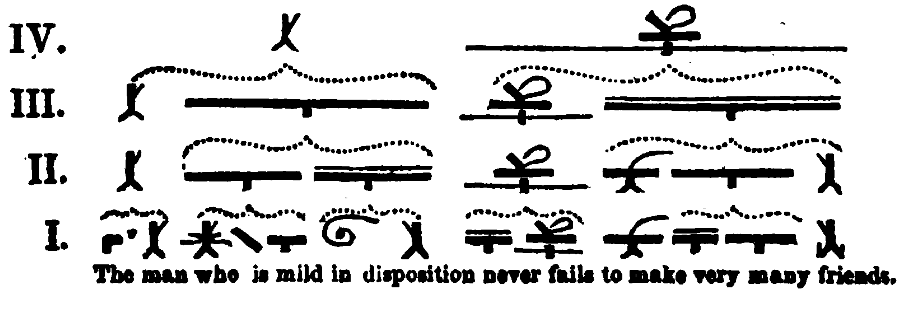
\includegraphics[width=\textwidth]{figures/vol1syntaxe2-img019.png}

    \textbf{Diagramme de Barnard\\}
    \textit{L’homme qui est doux de caractère n’échoue jamais à se faire de très nombreux amis}.

    De la même façon, la relative \textit{who is mild in disposition} ‘qui est doux de caractère’ se comporte comme un adjectif (cf. le symbole       également associé à \textit{mild} ‘doux’ et \textit{many} ‘nombreux’) et sa combinaison avec \textit{the man} ‘l’homme’ se comporte comme un nom (   ) ; de même, \textit{to make very many friends} ‘à se faire vraiment beaucoup d’amis’ se comporte comme un adverbe et sa combinaison avec \textit{never fails} ‘n’échoue jamais’ comme un verbe (        ). Par contre Barnard ne considère pas la proposition comme équivalente au verbe et reste avec une structure sujet-prédicat pour la proposition que l’on retrouve de la grammaire de Port-Royal à la grammaire générative (voir l’\encadref{fig:5.2.4} sur \textit{Fonctions syntaxiques et prédicat}). Le diagramme qu’il propose peut néanmoins être considéré comme un premier exemple d’arbre de constituants et même d’arbre de constituants avec tête, puisque les étiquettes indiquent la catégorie de la tête comme en syntaxe X-barre (voir l’\encadref{fig:3.4.19} sur la \textit{Syntaxe X-barre}).

    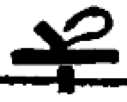
\includegraphics[width=\textwidth]{figures/vol1syntaxe2-img020.png}

    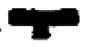
\includegraphics[width=\textwidth]{figures/vol1syntaxe2-img021.png}

    
\includegraphics[width=\textwidth]{figures/vol1syntaxe2-img022.png}

    Il semble que les contemporains de Barnard n’aient pas vraiment vu la portée de ces diagrammes et il faut attendre plus d’un siècle pour qu’en 1943, dix ans après la publication de \textit{Langage} de Bloomfield, Eugene Nida propose à nouveau des structures de constituants, dans une thèse intitulée \textit{A Synopsis of English Syntax}. Les structures proposées par Nida sont en fait des polygraphes (voir l’\encadref{fig:3.2.23} sur \textit{Graphe à bulles et polygraphe}) où chaque lien représente une connexion binaire et où les liens peuvent avoir pour sommet d’autres liens. Nida va ensuite enrichir son système en ajoutant des symboles sur les liens : les liens marquées d’une croix (X) représentent une construction exocentrique, tandis que les liens marqués d’une flèche (< ou >) représentent une construction endocentrique, la flèche pointant vers la tête. Dans le diagramme ci-dessous, \textit{the} et \textit{men} sont connectés par un lien > indiquant que \textit{the} dépend de \textit{men}, puis \textit{by} est lié à ce lien par un lien X indiquant que la construction n’a pas de tête. Une telle représentation est équivalente à un arbre de constituants binaire (voir la \sectref{sec:3.4.21} sur \textit{Arbre de constituants binaires et polygraphe}).


    Représentation syntaxique de Nida (exemple de 1966) \textit{Le voleur a été poursuivi par les hommes}
    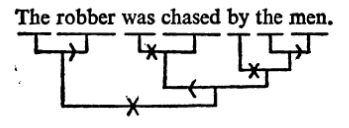
\includegraphics[width=\textwidth]{figures/vol1syntaxe2-img023.png}

    Une représentation similaire a été proposée dans les années 1950 par Charles Hockett (voir son ouvrage \textit{A course in modern linguistics} de 1958). Cette représentation, connue aujourd’hui sous le nom de \textstyleTermesapprof{boîtes de Hockett} n’est pas un arbre (au sens où les branches ne sont pas explicites), mais plutôt un emboîtement de constituants, assez proche de l’arbre de dépendance avec projections intermédiaires que nous avons présenté à la \sectref{sec:3.4.15} (sur \textit{Projections partielles et ordre de saillance}). Les unités de bases sont les syntaxèmes (on notera la décomposition de la forme verbale \textit{wants} en \textit{want}{}- \textrm{${\oplus}$}[F020?]{}-\textit{s}) et les intonèmes (les «~signes~» prosodiques) sont discrétisés (c’est-à-dire représentés par des symboles, ici 2, 3, 1 et ↓) et également intégrés à la décomposition. Il s’agit en fait d’une décomposition assez proche de la structure syntaxique X-barre qui ré-émergera 20 ans plus tard (voir l’\encadref{fig:3.4.19} sur la \textit{Syntaxe X-barre}), si ce n’est que Hockett considère encore que la combinaison \textit{sujet-verbe} est endocentrique. Le diagramme peut être enrichi de symboles \textrm{⧀} ou \textrm{⧁} indiquant, comme chez Nida, la dépendance.

    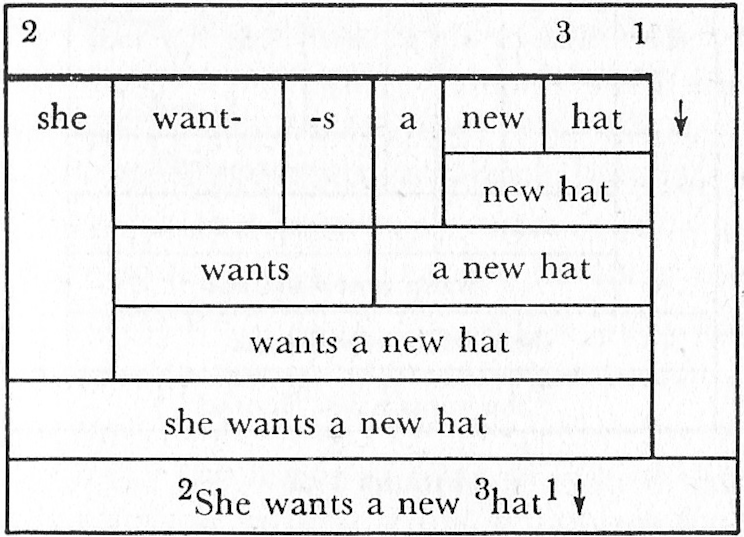
\includegraphics[width=\textwidth]{figures/vol1syntaxe2-img024.png}

    Représentations syntaxiques de \citealt{Hockett1958}
    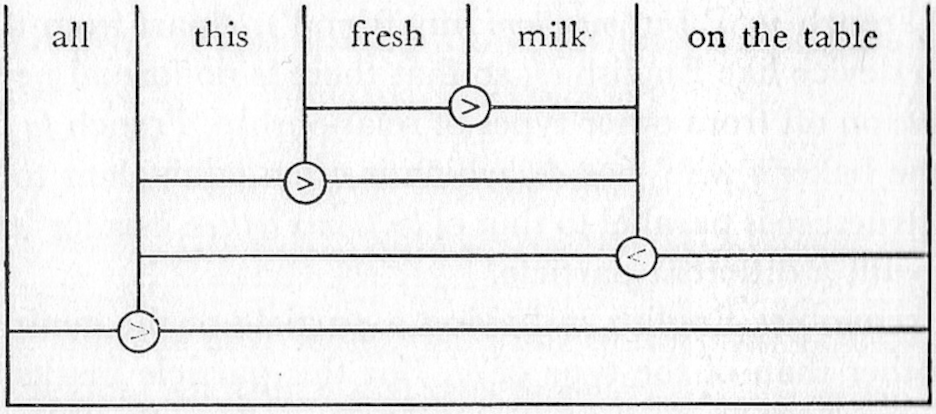
\includegraphics[width=\textwidth]{figures/vol1syntaxe2-img025.png}

    Dans cette représentation, chaque module de trois cases est à lire comme une \textbf{construction}, comme le remarque Hockett (dans le chapitre \textit{Form classes and constructions}) :

    \ea
    %%[Warning: Draw object ignored]
    %%[Warning: Draw object ignored]

    Construction chez Hockett            Construction dans un arbre de constituants avec tête
    \z


    Une telle analyse est contemporaine des grammaires de réécriture de Chomsky (voir l’\encadref{fig:3.5.30} sur la \textit{Grammaire de réécriture}) et son objectif est absolument similaire. On notera néanmoins que la représentation de Hockett met autant en avant la combinaison de A et B que la relation partie-tout de A ou de B avec le tout C qu’ils forment.

    On attribue généralement l’introduction des arbres de constituants à Chomsky. On en trouve dans son article de 1956, mais il est intéressant de noter que le diagramme en constituants introduit dans \textit{Syntactic Structures} de 1957 n’est pas stricto sensu un arbre. Ce diagramme, reproduit ci-dessous, apparaît dans le chapitre 4 intitulé \textit{Phrase structure} ‘Structure syntagmatique’, où Chomsky introduit les règles de réécriture, comme \textit{Sentence → NP + VP}. Dans le diagramme, il n’y a pas, comme dans les arbres de constituants ordinaires, de relations partie-tout entre le nœud \textit{Sentence} et les constituants immédiats \textit{NP} et \textit{VP}. Au lieu de cela, il y a un lien entre \textit{NP} et \textit{VP} correspondant au symbole + de la règle et que l’on peut interpréter comme un lien de connexion, ainsi qu’un lien entre le nœud \textit{Sentence} et le lien de connexion correspondant à l’opération de réécriture représentée par le symbole \textit{→} dans la règle. Le diagramme est donc un polygraphe.

    \ea
    \citealt{Chomsky1957}
    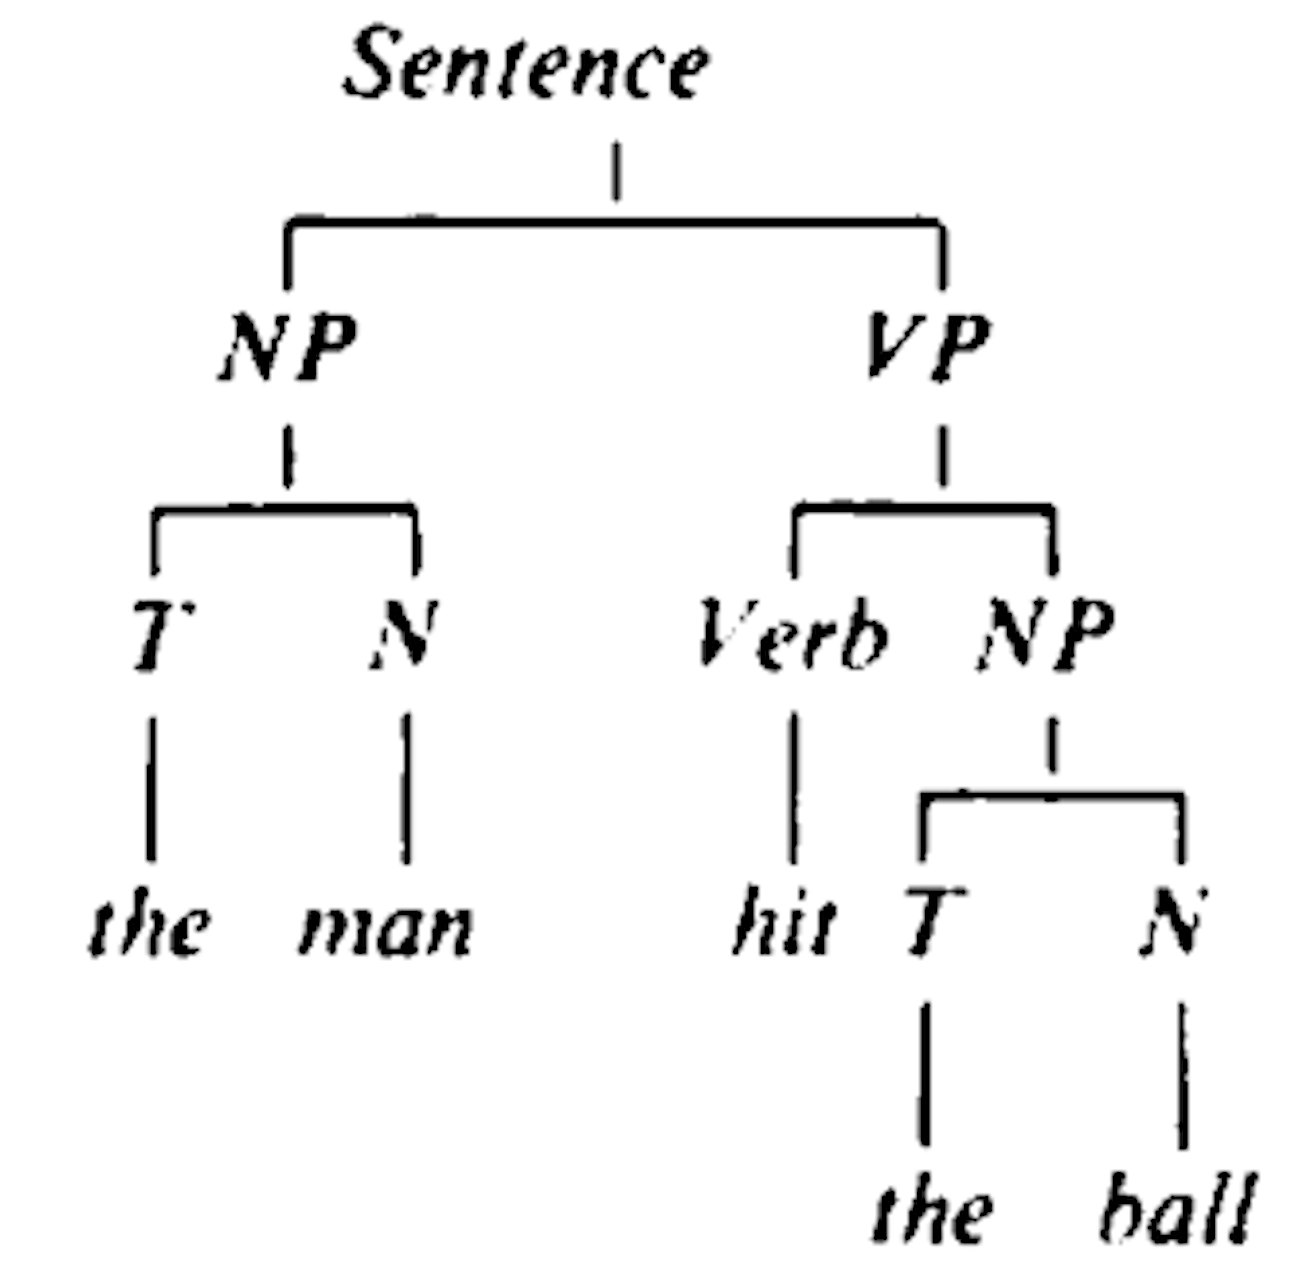
\includegraphics[width=\textwidth]{figures/vol1syntaxe2-img026.png}

    \z

    \ea
    \citealt{Chomsky1965}
    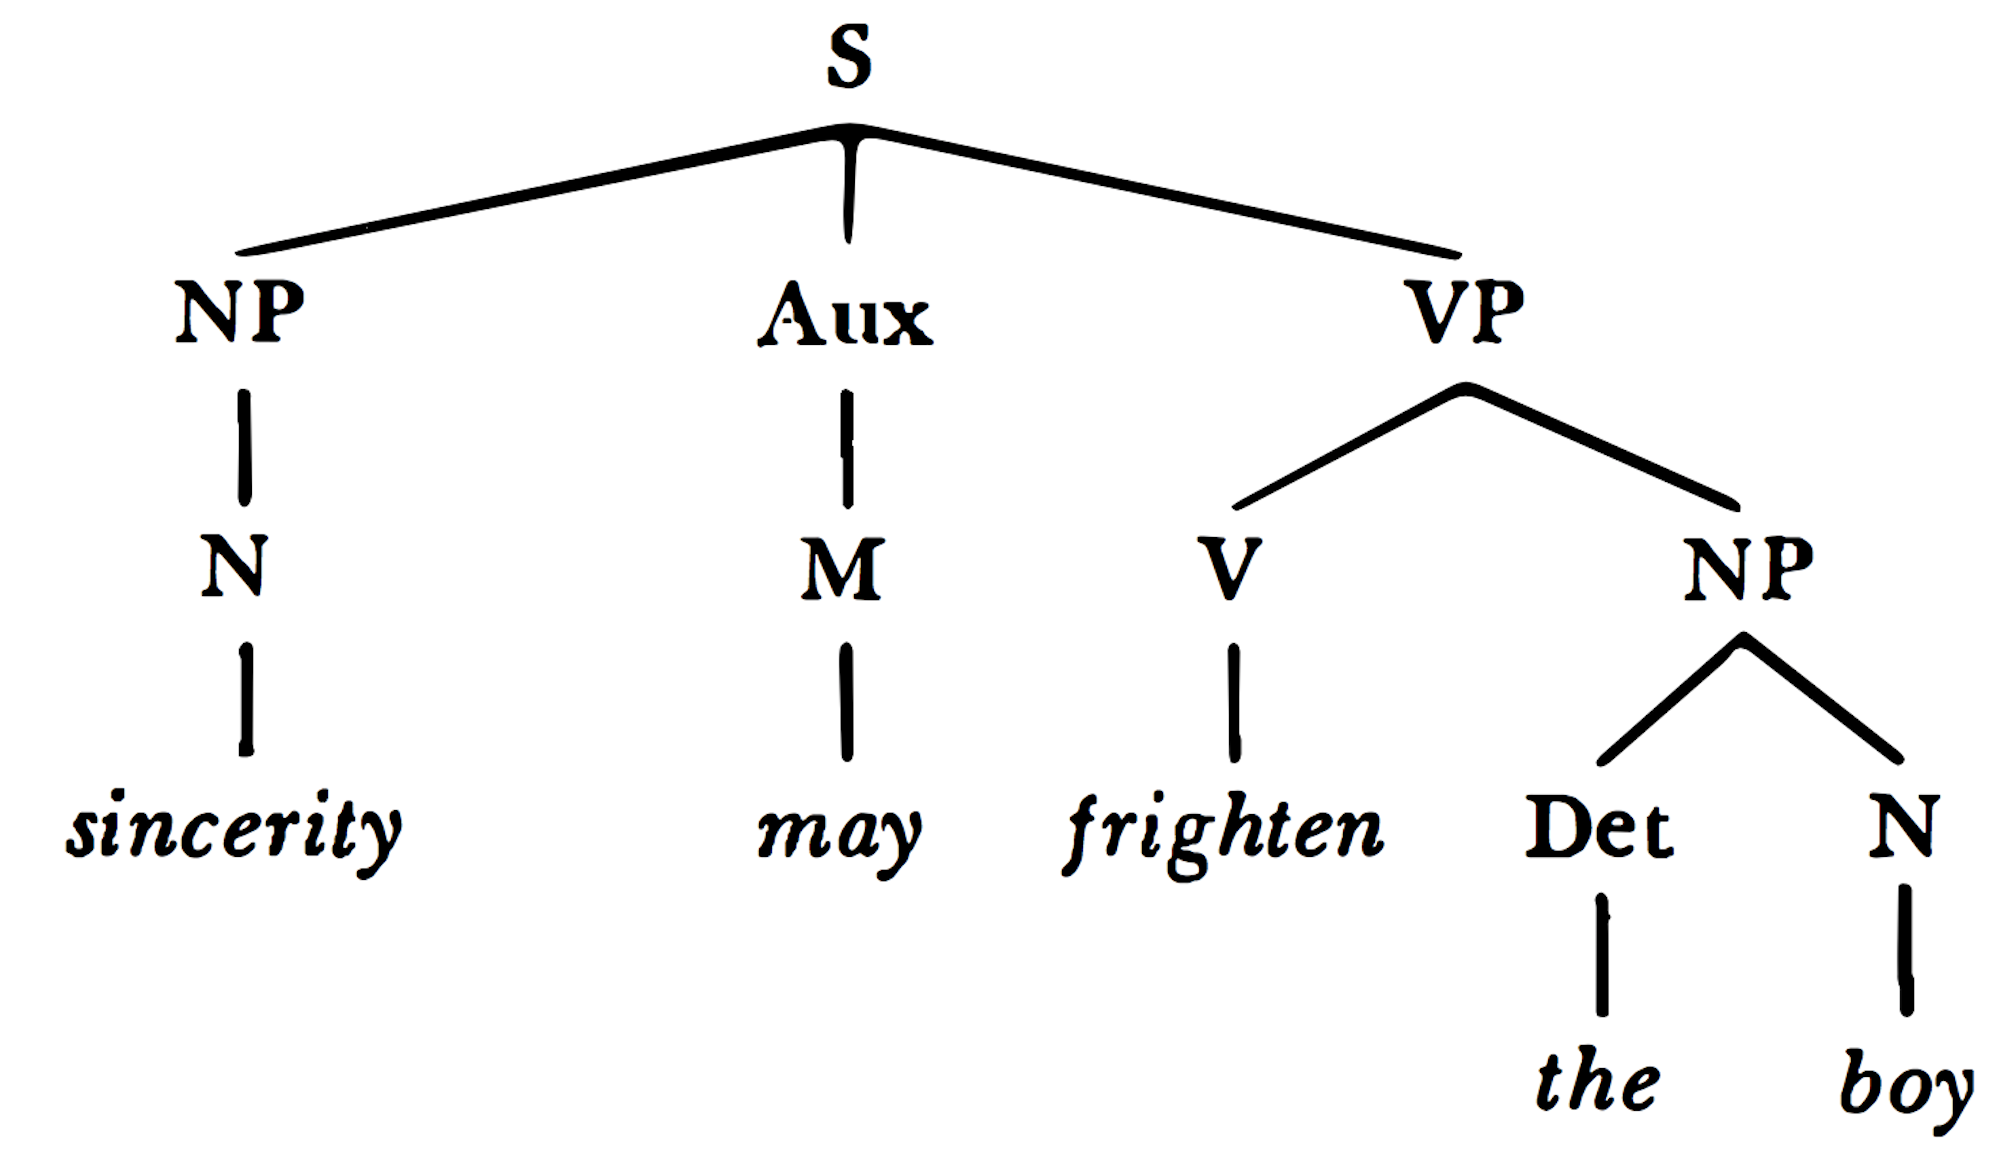
\includegraphics[width=\textwidth]{figures/vol1syntaxe2-img027.png}
    \z

    Dans son deuxième livre, \textit{Aspects of the Theory of Syntax}, publié en 1965, Chomsky revient à des arbres (voir l’exemple ci-dessus pour la phrase \textit{Sincerity may frighten the boy} ‘La sincérité peut effrayer le garçon’). On notera que si le diagramme de 1957 est fondamentalement binaire, la binarité n’est plus exigée dans les arbres de 1965. Elle réapparaîtra dans les travaux suivants et notamment la syntaxe X-barre.
}
\loupe{Binarité, construction et connexion}{%\label{sec:3.4.18}
    L’exigence de \textstyleTermesapprof{binarité} des arbres de constituants est antérieure à l’usage de la représentation en arbre. L’idée qu’une décomposition représente une \textstyleTermesapprof{construction} élémentaire est déjà bien présente dans \textit{Language} de Leonard \citet{Bloomfield1933}. Bloomfield donne l’exemple de la construction \textit{actor-action}, que l’on pourrait appeler la construction \textit{subjectale}, pour reprendre un terme proposé par Igor Mel’čuk \REF{ex:key:1988}. Autrement dit, il existe dans la phrase ordinaire une combinaison remarquable qui est celle du sujet avec le prédicat verbal (qu’on le conçoive comme le verbe seul ou comme un «~groupe verbal~», cela ne change rien pour nous, en termes de connexion). Cette construction (il s’agit bien d’une construction, au sens où on l’entend encore aujourd’hui, par exemple dans les \textstyleTermesapprof{Grammaires de constructions}) est bien binaire, mettant en relation deux éléments, le sujet et le prédicat verbal. Selon les formalismes, cette construction sera représentée par une connexion ou une décomposition :

    \ea
    %%[Warning: Draw object ignored]
    Trois représentations de la construction subjectale
    \z

    Le premier diagramme dit qu’il y a une unité dont la tête est un nom (N) qui dépend d’un verbe (V) par une relation \textit{sujet}, le deuxième diagramme \citep{Chomsky1957} dit qu’il y a un groupe nominal (NP, \textit{noun phrase}) et un groupe verbal (VP, \textit{verbal phrase}) qui se connecte pour former ensemble une phrase (S), tandis que le troisième diagramme dit que la phrase possède deux composantes, un NP et un VP. Même si cela n’apparaît pas au premier regard, il s’agit de trois représentations de la même construction. Qui plus est, ces trois descriptions sont moins éloignées qu’il n’y paraît à première vue comme on l’a déjà vu dans le \chapref{sec:3.2} sur la \textit{Connexion} et comme on le verra à nouveau dans la \sectref{sec:3.4.21} sur \textit{Arbre de constituants binaires et polygraphes}, puisqu’on passe de l’une à l’autre en réifiant ou déréifiant les relations partie-tout de la relation \textit{sujet}.

    L’exigence de binarité est une propriété partagée par de nombreuses analyses en constituants et par les analyses en dépendance : de la même façon que les constructions sont encodées par des \textbf{dépendances}, c’est-à-dire des \textbf{relations deux à deux des mots}, dans un arbre de dépendance, les constructions seront encodées par des \textbf{décompositions binaires}, c’est-à-dire des \textbf{relations deux à deux des constituants}, dans un arbre de constituants binaire.

    La principale différence dans les deux approches concerne la façon dont les différentes constructions sont repérées dans la structure. Dans le cadre de la syntaxe de dépendance, les constructions sont distinguées par l’étiquetage fonctionnel des dépendances (voir le \chapref{sec:5.2} sur les \textit{Fonctions syntaxiques}) et donc par une dénomination explicite de la construction : ainsi l’étiquette \textit{sujet} sur la dépendance plus haut indique-t-elle qu’il s’agit de la construction subjectale. Dans le cadre de la syntaxe de constituants, les primitives sont les catégories et le repérage entre les constructions est fait par la configuration et les catégories : ainsi le sujet est-il le NP sous S, tandis que l’objet est le NP sous VP :

    \ea
    %%[Warning: Draw object ignored]

    Deux représentations des constructions subjectale et objectale
    \z
}
\loupe{Syntaxe X-barre}{%\label{sec:3.4.19}
    La \textstyleTermesapprof{Syntaxe X-barre} est la version la plus aboutie de l’\textbf{analyse en constituants immédiats} (ACI) (voir la \sectref{sec:3.2.25} éponyme). Elle est développée à partir des années 1970 par Noam Chomsky et son étudiant Ray Jackendoff.

    L’innovation majeure de la Syntaxe X-barre est que \textbf{tout constituant} est considéré comme étant la \textbf{projection d’une} \textbf{tête}. Dans les versions précédentes de l’ACI, la phrase était décomposée en un groupe substantival et un groupe verbal (cf. la fameuse règle S \textrm{→} NP VP), ce qui en faisait un constituant exocentrique. Le fait que tout constituant ait une tête rend la Syntaxe X-barre extrêmement proche d’une analyse en dépendance. (Seule la coordination est encore parfois traitée comme une construction symétrique dont les conjoints sont les co-têtes ; voir \encadref{fig:3.4.26} sur les \textit{Deux types d’arbres de constituants}.)

    La deuxième caractéristique de la Syntaxe X-barre est que les \textbf{nœuds} \textbf{de base} sont des \textbf{syntaxèmes} et non des mots. Il y a donc deux types de constituants considérés, les \textbf{projections lexicales}, dont la tête est un lexème, et les \textbf{projections} dites \textbf{fonctionnelles} dont la tête est un syntaxème flexionnel (une catégorie fonctionnelle dans les termes de la Syntaxe X-barre).

    La troisième caractéristique de la Syntaxe X-barre est que l’arbre de constituant est \textbf{ordonné} et aucun constituant n’est discontinu, ce qui, pour les raisons que nous avons exposé dans l’\encadref{fig:3.2.7} \textit{De la non-séparation des ordres au mouvement}, entraîne la présence de nombreuses positions occupées par des traces co-indicés avec d’autres positions.

    La quatrième caractéristique de l’arbre X-barre est qu’il est \textbf{binaire}. Ainsi la combinaison de chaque dépendant avec son gouverneur correspond à une décomposition binaire différente, ce qui, d’une certaine façon, rapproche encore plus cet arbre d’un arbre de dépendance (voir l’\encadref{fig:3.4.18}). La conséquence est que si un syntaxème a beaucoup de dépendants, il sera la tête d’autant de projections. Si le syntaxème est de catégorie X, sa \textbf{projection maximale} est notée XP (\textit{X Phrase}) et ses \textbf{projections intermédiaires} X’ (à l’origine elles étaient notées avec une ou plusieurs barres au-dessus de X, d’où le nom de syntaxe X-barre).

    La Syntaxe X-barre considère de plus que l’élément sous XP a des propriétés différentes des éléments sous X’ : le premier est un \textbf{spécifieur}, alors que les autres sont des \textbf{compléments}. Dans certaines versions de la Syntaxe X-barre \citep{Jackendoff1977}, les ajouts (ou modifieurs) sont structurellement distingués des compléments actanciels par l’ajout d’un niveau de stratification supplémentaire dans la configuration de base (c’est-à-dire que XP porte une «~barre~» supplémentaire).

\ea{
    %%[Warning: Draw object ignored]
    }

    Configuration de base de la Syntaxe X-barre
    \z

    En conclusion, l’arbre de constituants de la Syntaxe X-barre est assez différent des arbres de constituants plats. Les deux sont des \textbf{arbres de constituants avec têtes}, mais le dernier ne contient que des projections maximales, qui, qui plus est, peuvent former des constituants discontinus. L’arbre X-barre ne repose pas vraiment sur des tests de constituance (qui, comme on l’a vu dans les encadrés 3.4.11-12, caractérisent essentiellement les projections maximales), mais sur des \textbf{principes configurationnels}. En d’autres termes, plus la géométrie d’un arbre permet de prédire de propriétés syntaxiques de l’énoncé qu’il représente, plus l’arbre a de raisons d’être. Ainsi, par exemple, le fait que le groupe substantival qui suit \textit{mange} possède des propriétés différentes dans les deux phrases suivantes devrait conduire à des configurations différentes, ce qui amène à compliquer à dessein la structure :

\ea{
    Pierre mange le pain.
    }
    \z

\ea{
    Pierre mange la nuit.
    }
    \z

    Dans l’approche que nous développons ici, ces deux énoncés auront la même «~structure~» syntaxique (c’est-à-dire le même squelette structurel), mais les groupes substantivaux \textit{le pain} et \textit{la nuit} auront des fonctions totalement différentes (voir \chapref{sec:5.2} sur les \textit{Fonctions syntaxiques}).

    On peut s’étonner du fait que la syntaxe X-barre dont l’objectif est de rendre compte des propriétés syntaxiques par des configurations géométriques n’ait pas cherché à encoder structurellement une notion aussi fondamentale que la notion de \textit{tête}, ce que font pourtant les structures de dépendance !
}
\loupe{Le groupe verbal}{%\label{sec:3.4.20}
    Le terme \textit{groupe verbal} (angl. \textit{verb phrase}, \textit{VP}) n’est pas utilisé de manière consistance dans la littérature. Ce terme désigne selon les auteurs deux notions différentes, que nous appellerons VP1 et VP2 :

    \begin{itemize}
    \item \textbf{VP1} \textbf{e}st une \textbf{projection partielle} de la \textbf{forme verbale} sans son sujet ;
    \item \textbf{VP2} est la \textbf{projection maximale} du \textbf{lexème verbal}.
    \end{itemize}
    Les deux notions sont souvent confondues, alors qu’elles renvoient à des constituants différents et à des cadres théoriques différents.

    VP2 est une notion théoriquement valable, mais qui suppose que l’on travaille avec la \textbf{granularité des syntaxèmes}. Il y a alors lieu de considérer que le sujet dépend plutôt de la flexion (voir la \sectref{sec:3.2.18} \textit{Structures de connexion, granularité et critères}) et donc VP2 est constitué du lexème verbal et de tous les éléments qu’il régit à l’exception du sujet. On notera néanmoins que VP2 n’est pas une unité autonomisable (puisque le lexème verbal n’apparaît jamais sans flexion) et qu’elle n’est donc qu’un objet théorique servant à expliciter, dans le cadre de l’analyse en constituants, que la réalisation du sujet davantage liée à la nature de la flexion qu’à celle du lexème. Il y a, à notre avis, des moyens plus simples et plus directs, d’indiquer le lien entre le sujet et la flexion verbale.

    \ea
    %%[Warning: Draw object ignored]
    VP1 est une notion sans grand intérêt théorique de notre point de vue. Il s’agit d’un constituant intermédiaire (VP1 est le I’ de l’analyse de droite ci-dessous), qui résulte d’une stratification qui nous semble peu justifiée. En effet, rien ne permet de considérer que la forme verbale se combine d’abord avec ses autres dépendants avant de se combiner avec son sujet et donc de donner ainsi un statut spécial au sujet.

    %%[Warning: Draw object ignored]
    Configurations syntaxiques caractérisant respectivement VP1 et VP2
    \z

    Dernière remarque qui pourrait expliquer l’introduction de VP1 dans les analyses en constituants : l’anglais (qui est la langue la plus étudiée et la plus enseignée) a un \textbf{constituant topologique} du type VP1 (voir les exercices du \chapref{sec:3.5}). Mais il est clair que la plupart des langues n’ont pas du tout cette configuration topologique et que, de toute façon, cela ne justifie pas l’introduction de VP1 dans la structure syntaxique au sens propre (que nous distinguons de la structure topologique).
}
\section{Arbre de constituants binaire et polygraphe}\label{sec:3.4.21}

Nous avons vu deux usages possibles de la représentation de la structure syntaxique par un arbre de constituants avec têtes : l’\textbf{arbre de constituants plat} et l’\textbf{arbre de constituants binaire}. (Nous confirmerons qu’il s’agit bien de deux usages différents du même formalisme dans l’\encadref{fig:3.4.25} sur \textit{Deux types d’arbres de constituants}, où nous montrons l’interprétation différente du branchement ternaire dans les deux conventions de représentation).

Nous avons vu que l’arbre de constituants plat pouvait être déduit trivialement (c’est-à-dire par un procédé de conversion automatique pure, sans ajout d’aucune information) d’un arbre de dépendance, ce qui n’est pas le cas de l’arbre de constituants binaire, qui nécessite d’ajouter un ordre de saillance sur les dépendances. Cela pourrait laisser penser que l’arbre de constituants plat est plus proche de l’arbre de dépendance : c’est vrai si on se place du point de vue formel, mais ça ne l’est pas si on se place du point de vue théorique. Comme on l’a vu dans les encadrés 3.4.15-16, il y a derrière l’\textbf{exigence de binarité}, le souci de dégager les différentes constructions syntaxiques, de les isoler les unes des autres. Et ce souci est commun avec les grammaires de dépendances. Nous allons montrer cela maintenant en repartant de notre exemple et de son arbre binaire le plus standard :

\begin{figure}
%%[Warning: Draw object ignored]

\caption{\label{fig:}Arbre de constituants binaire (avec têtes)}

\end{figure}

On peut interpréter chaque branchement binaire comme une connexion entre deux unités. Comme nous l’avons vu à la \sectref{sec:3.2.12} \textit{Représenter les combinaisons}, on peut représenter la combinaison A ${\oplus}$ B aussi bien par un lien entre A et B que par une bulle entourant A et B. Passer à un branchement binaire revient à \textbf{réifier} les relations partie-tout entre A et B et l’unité qu’ils forment ensemble (voir l’\encadref{fig:3.4.22} qui suit pour des compléments sur la notion de réification). Ici nous proposons de faire l’inverse, c’est-à-dire de \textbf{déréifier} les relations partie-tout qui constituent les branches d’un arbre de constituants. Comme en plus, chaque branchement binaire indique une tête (la branche T) et donne une connexion orientée, c’est-à-dire une dépendance :

\begin{figure}
%%[Warning: Draw object ignored]

\caption{\label{fig:}Passage d’un branchement binaire à une dépendance par déréification d’un nœud non terminal}

\end{figure}

Si l’on applique la déréfication à tous les nœuds intérieurs de l’arbre de constituants binaire, on obtient la structure suivante :

\begin{figure}
%%[Warning: Draw object ignored]

\caption{\label{fig:}Polygraphe orienté et ordonné}

\end{figure}

Cette structure est un \textstyleTermes{polygraphe} (voir définition formelle dans l’\encadref{fig:3.2.23} sur \textit{Graphe à bulles et polygraphe}) : ce n’est pas exactement un graphe, puisqu’un arc ne lie pas forcément deux nœuds (les nœuds sont les mots), mais il peut lier d’autres arcs entre eux ou un arc et un nœud. De plus, ce polygraphe est \textstyleTermes{orienté}, puisque chaque arc du graphe lie un gouverneur à un dépendant. Enfin ce polygraphe est implicitement \textstyleTermes{ordonné}, dans le sens où les nœuds du polygraphe sont disposés selon un ordre linéaire (celui des mots dans la phrase). De telles structures ont été proposées par le linguiste américain Eugene Nida dans sa thèse soutenue en 1943 (voir l’\encadref{fig:3.4.17} sur l’\textit{Historique des représentations syntaxiques par des diagrammes en constituants}.)

\maths{Réification et transitivité}{%\label{sec:3.4.22}
    Pour se fixer les idées sur la réification, donnons un autre exemple, emprunté à la représentation sémantique des constructions transitives. Considérons une phrase élémentaire telle que :

    \ea
    {Marie frappe Pierre.}
    \z

    Il y a là ce qu’on appelle un verbe transitif, \textit{frappe}, qui exprime une action d’un élément (\textit{Marie}) sur un autre (\textit{Pierre}). On dira encore que \textit{Marie} est l’\textbf{agent} de l’action et \textit{Pierre} le \textbf{patient}. Il y a alors plusieurs façons de représenter graphiquement le «~sens~» de cette phrase :

    \ea
    %%[Warning: Draw object ignored]
    \z

    Dans la représentation de gauche, \textit{frappe} est directement modélisé comme une action de Marie sur Pierre : \textit{frappe~}(\textit{Marie}, \textit{Pierre}). Dans celle du milieu, les relations qui lient \textit{frappe} à \textit{Marie} et \textit{Pierre} sont explicitées et nommées \textit{agent} et \textit{patient}. Dans celles de droite, les relations agent et patient sont vues comme des objets à part entière reliant les mots de la phrase : agent~(\textit{Marie}, \textit{frappe}) + patient~(\textit{Pierre}, \textit{frappe}). On l’aura deviné, les trois représentations sont des réifications successives des relations d’une même structure.

    Si toute structure peut-être réifiée à l’infini, comment choisir le bon niveau de réification ? Faire de la relation entre deux objets un objet n’a d’intérêt que si l’on veut la considérer en tant que telle et lui attribuer des propriétés. Dans le cas de la transitivité, on peut préférer la représentation du milieu qui explicite les relations d’agent et de patient et permet donc d’en parler, par exemple pour décrire la voix passive (voir le \chapref{sec:3.6}).

    Dans le cas de la relation de connexion, nous pensons qu’il n’est pas nécessaire d’expliciter les relations partie-tout que la connexion entretient avec les unités qu’elle connecte.
}
\section{Polygraphe orienté et arbre de dépendance}\label{sec:3.4.23}

Si l’on s’abstrait complètement de l’ordre linéaire et que l’on garde uniquement le polygraphe orienté, on peut adopter la représentation suivante, où chaque arc est représenté par une ligne droite avec le gouverneur au-dessus de son dépendant :

\begin{figure}
%%[Warning: Draw object ignored]

\caption{\label{fig:}Polygraphe orienté (non ordonné)}

\end{figure}

Bien que cela n’apparaisse pas au premier coup d’œil, la structure ci-dessus est un extrait de la structure précédente : c’est le même \textbf{polygraphe orienté} que précédemment, mais sans l’ordre des mots et avec une autre convention de représentation : au lieu d’indiquer la tête de la connexion par une flèche, celle-ci est placée au-dessus de son dépendant. Or ce polygraphe orienté, qui a donc été extrait automatiquement de l’arbre de constituants binaires en mettant en évidence les connexions, est très proche d’un arbre de dépendance. Pour obtenir l’arbre de dépendance, il suffit de \textbf{faire glisser chaque dépendance} le long des dépendances sur lesquelles elle s’appuie:

\begin{figure}
%%[Warning: Draw object ignored]

\caption{\label{fig:}«~Glissade~»}

\end{figure}

Nous retombons finalement sur notre arbre de dépendance :

\begin{figure}
%%[Warning: Draw object ignored]

\caption{\label{fig:}Retour à l’arbre de dépendance (bis)}

\end{figure}

Nous appellerons \textstyleTermes{méthode par déréification }la méthode que nous venons de présenter, qui permet de passer d’un arbre de constituants binaire avec têtes à un arbre de dépendance.

La méthode par déréification peut s’appliquer à des arbres de constituants dont certains branchements décrivent des constructions exocentriques et n’ont donc pas de marquage de la tête.

Dans l’exemple suivant (déjà étudié dans la \sectref{sec:3.3.23} \textit{Nom ou déterminant comme tête} ?), \textit{le petit chien dort}, si on ne décide pas qui de l’article \textit{le} ou du nom \textit{chien} est la tête du groupe substantival, on obtient par déréification une connexion non orientée, qu’on ne peut pas faire «~glisser~» comme on l’a fait précédemment pour les connexions orientées.

\begin{figure}
%%[Warning: Draw object ignored]

  Arbre de constituants                Structure de dépendance

               \textbf{avec marquage partiel des têtes}               \textbf{associée}
\caption{\label{fig:}}
\end{figure}

Nous retombons sur les structures de dépendance que nous avions proposé pour les constructions exocentriques au \chapref{sec:3.3}.

\section{Comparaison des méthodes par décomposition}\label{sec:3.4.24}

Nous avons présenté deux \textbf{méthodes par décomposition} pour passer d’un arbre de constituants à un arbre de dépendance : la méthode de Lecerf ou méthode par agrégation des projections d’une part et la méthode par déréification d’autre part.

Les deux méthodes sont différentes et s’appliquent à des types d’arbres de constituants différents : la \textbf{méthode de Lecerf} s’applique uniquement à des arbres de constituants avec têtes, puisqu’elle repose crucialement sur l’agrégation des projections d’une même \textbf{tête~}; la \textbf{méthode par déréification} s’applique à n’importe quel type d’arbre de constituants, mais elle ne donne des \textbf{connexions binaires} que si elle est appliquée à un arbre binaire (voir l’\encadref{fig:3.4.26} pour le cas des branchements ternaires).

Néanmoins lorsque les deux méthodes sont appliquées au même arbre de dépendance \textbf{binaire avec têtes}, elles donnent le \textbf{même arbre de dépendance} (voir exercices).

\section{Équivalences entre structures}\label{sec:3.4.25}

Nous avons présenté un grand nombre de structures plus ou moins équivalentes. La figure suivante rassemble ces différentes structures.

La partie droite de la figure montre le passage d’un arbre de dépendance à \textbf{un arbre de constituants plat}, puis retour à l’arbre de dépendance, tandis que la partie gauche montre le passage d’un arbre de dépendance à un \textbf{arbre de constituants binaire avec têtes}, puis retour à l’arbre de dépendance.

\begin{figure}
\caption{\label{fig:}}
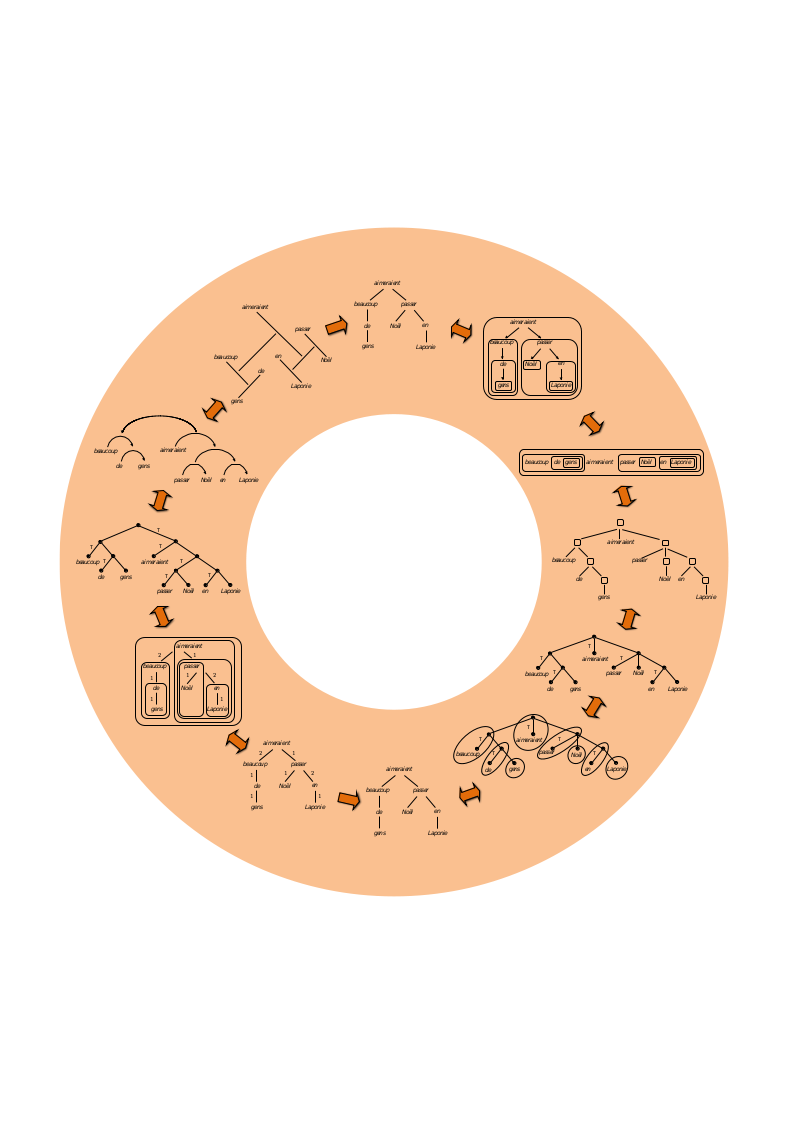
\includegraphics[width=\textwidth]{figures/vol1syntaxe2-img028.png}
\end{figure}

Chaque flèche entre deux structures symbolise une opération élémentaire permettant de passer d’une structure à une autre. Dans la plupart des cas, l’opération ne nécessite l’ajout d’aucune information et les deux structures sont équivalentes (nous ne considérons pas l’ordre linéaire sur les mots qui est des fois présent dans la structure et d’autres fois non). C’est le cas dans toute la partie droite de la figure, où toutes les structures sont équivalentes entre elles. De la même façon, toutes les structures de la partie gauche sont équivalentes entre elles. Elles contiennent une information supplémentaire qui est la stratification. Cette stratification, qui permet de stratifier les branchements non binaires, est indiquée dans la partie basse de la figur    e par l’ajout de l’ordre de saillance, lequel disparaît dans la partie haute, lorsque les «~glissades~» sont effectuées sur le polygraphe et qu’on revient à l’arbre de dépendance.

\loupe{Deux types d’arbres de constituants}{%\label{sec:3.4.26}
    Nous avons présenté dans ce chapitre deux types d’arbres de constituants avec têtes : les arbres de constituants plats et les arbres de constituants binaires comme ceux de la syntaxe X-barre. On peut penser que tout arbre de constituants plat peut être «~binarisé~» en introduisant des constituants intermédiaires. En fait, la différence est plus profonde et il s’agit à notre avis de deux façons assez différentes d’utiliser le même formalisme. La différence apparaît lorsqu’on regarde les branchements ternaires.

    Dans un arbre plat, les branchements ternaires sont courants. Ils apparaissent dès qu’un mot a deux dépendants. Reprenons l’exemple de \textit{passer Noël en Laponie}, qui se décompose en trois morceaux, une tête (\textit{passer}) et ses deux dépendants (\textit{Noël} et \textit{en Laponie}) (voir la section sur les \textit{Arbres de constituants avec têtes plats}).

    \ea
    %%[Warning: Draw object ignored]
    \z

    Branchement ternaire et correspondance par la méthode de Lecerf

    En appliquant la méthode de Lecerf à l’arbre plat de gauche, on obtient l’arbre de dépendance à droite. Comme on le voit, le branchement ternaire est interprété comme deux connexions binaires, la connexion entre \textit{passer} et \textit{Noël} et la connexion entre \textit{passer} et \textit{en Laponie}.

    Dans un arbre binaire, il en va tout autrement, puisque, comme nous l’avons montré ci-dessus (\sectref{sec:3.4.21} sur \textit{Arbres de constituants binaire et polygraphe}), chaque branchement correspond à une unique connexion. Si un tel arbre contient un branchement ternaire, il doit être interprété comme une \textbf{connexion ternaire} (voir l’\encadref{fig:3.2.17} \textit{Connexion binaire} ?). La syntaxe X-barre, qui revendique l’usage des arbres binaires, s’est aventurée à proposer des branchements ternaires pour la coordination (voir \citealt{Jackendoff1977}, mais on trouve déjà les mêmes arbres dans \citealt{Hockett1958} ; voir ci-dessous les boîtes de Hockett pour la coordination où le branchement est ternaire et symétrique, avec une position bien différenciée pour la conjonction).

    \ea
    %%[Warning: Draw object ignored]

    Branchement ternaire dans une boîte de Hockett
    \z

    C’est ce qu’on appelle l’analyse symétrique de la coordination (voir le \chapref{sec:5.3}) : dans \textit{Marie et Pierre dorment}, les conjoints (c’est le nom que l’on donne aux éléments coordonnés, \textit{Marie} et \textit{Pierre}) sont considérés comme des co-têtes, qui contribuent à égalité à la distribution du syntagme (lequel déclenche un accord pluriel du verbe). Il s’agit alors d’une construction ternaire, que nous pouvons représenter par une connexion ternaire en suivant les conventions de représentation utilisées par Tesnière dans son article de 1934 \textit{Comment construire une syntaxe} ?) : les deux conjoints \textit{Marie} et \textit{Pierre} sont au même niveau, reliés par une connexion horizontale, et la conjonction, qui est le troisième «~sommet~» de cette connexion, est placé en dessous.

    \ea
    %%[Warning: Draw object ignored]

    Branchement ternaire et correspondance par la méthode de déréification
    \z

    La structure de dépendance de droite peut être obtenue en appliquant la méthode de conversion par déréification à l’arbre de constituant à gauche. Le branchement ternaire donne une connexion ternaire, où \textit{Marie} et \textit{Pierre} occupent des positions symétriques (puisqu’ils sont co-têtes), tandis que la conjonction \textit{et} occupe une troisième position, comme «~dépendant~» des co-têtes. La convention de Tesnière rend bien compte de cela.

    En conclusion, on note que \textbf{le formalisme des arbres de constituants est ambigu~}: il ne permet pas de distinguer une analyse plate (on ne souhaite pas considérer de constituants intermédiaires) et une connexion ternaire (on souhaite indiquer que les éléments ne se combinent pas toujours deux à deux, mais parfois par trois). Celui des structures de dépendance le permet, à condition de considérer des structures qui ne sont plus des arbres et qui contiennent des connexions ternaires.
}
\section{Combiner les méthodes ascendante et descendante}\label{sec:3.4.27}

A l’issu de ce chapitre et des deux précédents, nous avons présenté plusieurs méthodes pour construire la structure syntaxique. Nous aimerions conclure ce chapitre en montrant comment combiner les méthodes ascendante (par combinaison) et descendante (par décomposition). Notre présentation visait jusque-là à montrer le bien-fondé d’un certain nombre de représentations syntaxiques et leurs équivalences totales ou partielles. Mais nous n’avons pas suffisamment montré comment les différentes méthodes peuvent interagir et comment, en pratique, on peut procéder pour construire une représentation syntaxique lorsqu’on est confronté à un texte à analyser.


Nous allons prendre un exemple (on peut démarrer avec des exemples plus simples~[F04A?]) (tiré des \textit{Fleurs du mal} de Beaudelaire, \textit{La vie antérieure}) :

\ea{
C’est là que j’ai vécu dans les voluptés calmes,
}
\z
\ea{
Au milieu de l’azur, des vagues, des splendeurs
}
\z
\ea{
Et des esclaves nus, tout imprégnés d’odeurs,
}
\z
\ea{
Qui me rafraîchissaient le front avec des palmes,
}
\z
\ea{
Et dont l’unique soin était d’approfondir
}
\z
\ea{
Le secret douloureux qui me faisait languir.
}
\z

Nous allons analyser cet exemple en procédant aussi bien par décomposition que par combinaison. Nous pouvons effectuer quatre types d’opérations.

\begin{itemize}
\item \begin{styleLivreImportant}
Nous pouvons repérer des \textbf{unités syntaxiques}, pas seulement des projections maximales ou partielles. Toute unité repérée peut être parenthésée ou entourée d’une bulle.
\end{styleLivreImportant}
\end{itemize}

Illustration sur notre exemple : on peut par exemple s’appuyer sur la prosodie, la ponctuation ou, dans le cas d’un poème comme ici, sur le découpage en vers. Ces unités sont, en raison de leur autonomisabilité prosodique, des unités syntaxiques. En considérant que les vers et que les segments entre deux virgules sont des unités, nous obtenons le parenthésage suivant :

\ea{}
[ \textit{c’est là que j’ai vécu dans les voluptés calmes} ]

[ [ \textit{au milieu de l’azur} ] [ \textit{des vagues} ] [ \textit{des splendeurs} ] ]

[ [ \textit{et des esclaves nus} ] [ \textit{tout imprégnés d’odeurs} ] ]

[ \textit{qui me rafraîchissaient le front avec des palmes} ]

[ \textit{et dont l’unique soin était d’approfondir} ]

[ \textit{le secret douloureux qui me faisait languir} ]
\z

Plein d’autres découpages sont possibles. On voit en tout cas que même si notre exemple paraissait très complexe au départ, on s’est maintenant ramené à l’étude de segments beaucoup plus raisonnables.

\begin{itemize}
\item \begin{styleLivreImportant}
Nous pouvons repérer des \textbf{connexions} entre unités. Dès qu’une connexion est repérée, on peut tracer un arc entre deux bulles.
\end{styleLivreImportant}
\end{itemize}

Notre exemple est finalement assez simple, puisque chacune des unités que nous avons dégagées à la première étape se connecte à la précédente !

\ea{}
[ \textit{c’est là que j’ai vécu dans les voluptés calmes} ]

—[ [ \textit{au milieu de l’azur} ]—[ \textit{des vagues} ]—[ \textit{des splendeurs} ] ]

—[ [ \textit{et des esclaves nus} ]—[ \textit{tout imprégnés d’odeurs} ] ]

—[ \textit{qui me rafraîchissaient le front avec des palmes} ]

—[ \textit{et dont l’unique soin était d’approfondir} ]

—[ \textit{le secret douloureux qui me faisait languir} ]
\z

Pour vérifier que deux unités se connectent bien, il suffit de vérifier que leur combinaison donne un segment autonomisable.

\begin{itemize}
\item \begin{styleLivreImportant}
Pour tout unité syntaxique, nous pouvons repérer sa \textbf{tête} et, par exemple la souligner.
\end{styleLivreImportant}
\end{itemize}

Cette étape est plus complexe et amène à des discussions. Il faut en particulier décider quel élément est la tête dans des groupes coordonnés comme [~\textit{et des esclaves nus~}] ou dans une proposition relative comme [~\textit{qui me rafraîchissaient le front avec des palmes~}]. Voir pour cela les chapitres 5.3 et 5.4. Pour d’autres unités, sans être forcément triviale, la question peut être rapidement résolue en appliquant les tests : par exemple la tête de [~\textit{tout imprégnés d’odeurs~}] est \textit{imprégnés} car \textit{tout} est effaçable et \textit{d’odeurs} est régi par le verbe \textsc{imprégner} dont il est le complément d’agent (\textit{les odeurs imprègnent quelque chose}). Nous différons donc certaines décisions et obtenons pour le début de notre exemple :

\ea{}
[ \textit{c’est là que j’ai vécu dans les voluptés calmes} ]

—[ [ \textit{à le milieu de l’azur} ]—[ \textit{de les vagues} ]—[ \textit{de les splendeurs} ] ]

—[ [ \textit{et de les esclaves nus} ]—[ \textit{tout imprégnés d’odeurs} ] ]
\z

On aura noté que certaines formes qui étaient des amalgames ont été décomposées. On vérifie en particulier que \textit{des} contient bien la préposition \textsc{de} par la commutation avec \textit{de ces}.

\begin{itemize}
\item \begin{styleLivreImportant}
Pour toute connexion, nous pouvons repérer sa tête et la hiérarchiser pour en faire une \textbf{dépendance}.
\end{styleLivreImportant}
\end{itemize}

La première unité contient le verbe principal de la phrase et est donc la racine de la structure, ce qui nous hiérarchise un certain nombre de connexions. Pour les autres, le critère d’effacement suffit.
\ea{}
[ \textit{c’est là que j’ai vécu dans les voluptés calmes} ]

→ [ [ \textit{à le milieu de l’azur} ] → [ \textit{de les vagues} ] → [ \textit{de les splendeurs} ] ]

→ [ [ \textit{et de les esclaves nus} ] → [ \textit{tout imprégnés d’odeurs} ] ]
\z
Ces différentes étapes peuvent bien sûr être réalisées à tour de rôle et à plusieurs reprises :

\begin{itemize}
\item \begin{styleLivreImportant}
A chaque fois qu’une unité est décomposée en de nouvelles unités, on pourra chercher à \textbf{raffiner les connexions} qu’elle entretient. Quand toutes les connexions d’une unité auront été attribuées à ses sous-unités, on pourra même effacer les frontières de cette unité.
\end{styleLivreImportant}
\end{itemize}

Ainsi les frontières de l’unité [~et des esclaves nus tout imprégnés d’odeurs~] peuvent être effacées dès qu’on a établi que [et de les esclaves nus] se combinent avec [de les splendeurs].
\ea{}
[ \textit{c’est là que j’ai vécu dans les voluptés calmes} ]

→ [ \textit{à le milieu de l’azur} ] → [ \textit{de les vagues} ] → [ \textit{de les splendeurs} ]

→ [ \textit{et de les esclaves nus} ] → [ \textit{tout imprégnés d’odeurs} ]

                                             $\searrow $ [ \textit{qui me rafraîchissaient le front …} ]
\z

\begin{itemize}
\item \begin{styleLivreImportant}
Dès qu’on a repéré la tête d’une unité, on pourra plus facilement en trouver les sous-unités (voir la \sectref{sec:3.4.6} sur \textit{Construire un arbre de dépendance par décomposition}).
\end{styleLivreImportant}
\end{itemize}

Par exemple, une fois repérée la tête de [~\textit{tout imprégnés d’odeurs~}], on a immédiatement :

\ea
{tout} ← \textit{imprégnés} → [ \textit{d’odeurs} ]
\z

Nous arrêtons là l’analyse de notre exemple. Les grands principes de l’analyse ont été donnés et nous terminons avec quelques remarques générales.

\section{Enseigner la syntaxe}\label{sec:3.4.28}

Les enseignements de syntaxe formelle se limitent en général à une partie des moyens qui précèdent. Lorsqu’on travaille en syntaxe de constituants, on demandera aux étudiants de reconnaître des projections, principalement maximales. Cela signifie que, parmi les quatre outils qui précèdent, on ne s’autorisera que l’usage du premier à savoir repérer des unités, et en plus il faudra se limiter à certaines unités seulement.

Les enseignements traditionnels en syntaxe de dépendance, eux, proposent de tracer des dépendances entre mots. Cela signifie que parmi les moyens précédents, on se limitera à tracer des connexions, uniquement entre mots, et à les orienter.

Nous proposons pour notre part de combiner tous les moyens. \textbf{Toute unité syntaxique est bonne à repérer}. Il n’est pas nécessaire de se limiter aux mots, comme en syntaxe de dépendance ou aux projections comme en syntaxe de constituants. Certaines séquences du type (Prép) (Dét) (Adj)* N (Adj)* (préposition-déterminant-nom, avec éventuellement des adjectifs avant ou après le nom) sont très facilement repérables (voir la discussion sur les \textstyleTermes{amas} à la \sectref{sec:3.5.35} sur les \textit{Constituants topologiques intermédiaires}). On pourra donc commencer par entourer les séquences de ce type. C’est ce que nous avons fait lorsque nous avons analysé \textit{la faible déclivité de la vallée de la Seine en Ile-de-France} dans la \sectref{sec:3.3.18} sur les \textit{Tests pour la connexion}. Si l’on prend notre exemple précédent, il est difficile pour un novice de repérer immédiatement le groupe substantival \textit{les esclaves nus, tout imprégnés d’odeurs, qui me rafraîchissaient le front avec des palmes, et dont l’unique soin était d’approfondir le secret douloureux qui me faisait languir}, alors qu’on repèrera beaucoup plus facilement les différents amas qui constituent ce groupe : [~\textit{les esclaves nus~}], [~\textit{tout imprégnés d’odeurs} ], etc. C’est seulement à la fin de l’analyse, quand toutes les unités auront été connectées, que le groupe substantival en entier émergera.

Nous pensons que le moyen le plus élégant pour représenter la structure finale est d’utiliser une structure de dépendance (et nous espérons en avoir convaincu le lecteur ; voir aussi l’\encadref{fig:3.4.29}). Il n’y a néanmoins aucune raison de proscrire les méthodes de l’analyse en constituants, bien au contraire. Il est tout à fait possible de combiner les deux méthodes et de gagner ainsi en simplicité. L’arbre de Beauzée-Gladkij est notamment une représentation que les novices en syntaxe formelle comprennent bien et qui est moins abstraite pour eux qu’un pur arbre de constituants ou un pur arbre de dépendance. Cette représentation a en plus l’avantage de présenter simultanément les constituants et les dépendances et d’être ainsi le support idéal pour une discussion sur la distinction entre catégories et relations syntaxiques (voir chapitres 5.1 et 5.2).

Pour conclure, insistons encore une fois sur le fait qu’il n’y a pas une méthode unique pour découvrir la structure syntaxique d’un énoncé. On peut procéder aussi bien de \textbf{manière descendante} (\textbf{décomposer une unité}, notamment en repérant sa tête) comme de \textbf{manière ascendante} (\textbf{connecter deux unités} pour former une unité plus grande).

\loupe{Constituance ou dépendance ?}{%{\label{sec:3.4.29}
    Nous avons montré dans ce chapitre que les arbres de dépendance et les arbres de constituants avec têtes étaient deux modes de représentation de la structure syntaxique plus ou moins équivalents : les deux types de structures rendent compte de la façon dont les unités se combinent ou se décomposent (les connexions) et du fait que ces combinaisons sont généralement asymétriques et forment une structure hiérarchique (les têtes et les dépendances). Malgré cette équivalence formelle, les deux types de structures ont des implications théoriques différentes. Nous allons discuter ici des conséquences de cette différence en voyant les avantages et inconvénients des deux types de structures.

    \section*{Têtes syntaxiques}

    Nous avons déjà souligné (voir la \sectref{sec:3.4.15} sur \textit{Projections partielles et ordre de saillance}) que les arbres de dépendance mettent en avant la notion de tête, qui est encodée configurationnellement par les dépendances, alors que les arbres de constituants avec têtes mettent en avant l’ordre de saillance (dans leur version binaire, c’est-à-dire stratifiée). Etant donné l’importance de la notion de tête, nous pensons que c’est là un avantage fort pour les arbres de dépendances.

    \section*{Constructions exocentriques    }

    La possibilité de ne pas encoder de tête ou de considérer des co-têtes est généralement considérée comme un avantage des arbres de constituants. Nous avons vu au chapitre précédent et à nouveau ici qu’il est tout a fait possible de considérer des connexions non hiérarchisées, à côté de dépendances (c’est-à-dire des connexions hiérarchisées), dans une structure de dépendance. Cela suppose néanmoins de travailler avec des polygraphes, c’est-à-dire des «~graphes~» où des arêtes peuvent relier d’autres arêtes, tandis que cela peut être encodé dans un arbre de constituants sans perdre la structure d’arbre. C’est la contrepartie du fait que la notion de tête n’est pas encodée configurationnellement dans les arbres de constituants.

    \section*{Unités syntaxiques}

    Les arbres de constituants mettent en avant certaines unités syntaxiques, à savoir les projections maximales, ainsi que des projections intermédiaires lorsque l’arbre est stratifié. Les arbres de dépendance considèrent également les projections maximales (qui correspondent aux sous-arbres de l’arbre de dépendance). Les arbres de dépendance permettent par ailleurs de considérer toutes sortes d’autres unités syntaxiques : en fait toute portion connexe de l’arbre de dépendance est une unité syntaxique potentielle (voir au chapitre précédent la définition de la \textit{Structure de connexion}). Il ne semble pas de ce point de vue que les projections intermédiaires des grammaires de constituants soient des unités plus intéressantes que les autres, comme le montre le fait qu’elles ne vérifient en général aucun des tests de constituance. Par contre, d’autres unités, comme les nucléus (voir le \chapref{sec:5.4} sur l’\textit{Extraction}), jouent un rôle important dans la grammaire. Or les nucléus, qui sont des chaînes immédiatement visibles dans l’arbre de dépendance, sont beaucoup plus cachés dans un arbre de constituants.

    \section*{Connexions}

    Les connexions sont présentes dans les deux structures, mais les arbres de dépendance combinent des mots ou des syntaxèmes, tandis que les arbres de constituants combinent des constituants. Autrement dit, les instances des connexions sont plus fines dans un arbre de dépendance que dans un arbre de constituants. Ceci est pour nous un avantage majeur des arbres de dépendance.

    Notons par ailleurs que si le dépendant d’une connexion est en général la projection maximale, c’est-à-dire un constituant, ce n’est pas toujours le cas. Comparons :

    \ea
    {Les linguistes qui étaient fatigués ont quitté la conférence.}
    \z

    \ea
    Les linguistes, qui étaient fatigués, ont quitté la conférence.
    \z

    Si dans le premier exemple, le sujet du verbe doit être compris comme le constituant \textit{les linguistes qui étaient fatigués}, dans le deuxième exemple, \textit{qui étaient fatigués,} bien qu’étant toujours dépendant de \textit{les linguistes} ne fait plus vraiment partie du sujet du verbe \textit{ont quitté}. Il y a deux prédications indépendantes sur \textit{les linguistes~}: d’une part, \textit{les linguistes ont quitté la conférence}, et d’autre part, \textit{les linguistes étaient fatigués}, qui est au second plan et sert de justification à la prédication principale.

    \section*{Ordre des mots}

    L’ordre des mots est plus facilement lisible dans un arbre de constituants, à tel point qu’il est même difficile d’envisager l’arbre de constituants indépendamment de l’ordre linéaire. Nous adoptons nous-mêmes un arbre de constituants pour représenter la structure topologique (voir chapitre suivant). Nous pensons par contre que les combinaisons syntaxiques doivent être clairement distinguées des relations de contiguïtés (voir la \sectref{sec:3.2.6} sur \textit{Structures syntaxiques et structures topologiques}) et que ne pas le faire conduit immanquablement à introduire la notion de mouvement (voir la \sectref{sec:3.2.7} \textit{De la non-séparation des ordres au mouvement}). En d’autres termes, les arbres de constituants peinent à rendre compte simplement des \textbf{structures non projectives}, sauf à introduire la notion de \textbf{constituant discontinu}, qui fait alors perdre tous les avantages de l’arbre de constituants du point de vue de l’ordre des mots. Le \chapref{sec:3.5} sera entièrement consacré à ces questions et à la définition d’une structure de constituants topologique distincte de la structure syntaxique.

    \section*{Interface sémantique-syntaxe}

    Nous avons vu aux chapitres \ref{sec:1.2} et \ref{sec:2.3} qu’une partie de la sémantique des énoncés pouvaient être saisie par un graphe de relations prédicat-argument, lequel graphe s’apparente à une structure de connexion, c’est-à-dire à un arbre de dépendance dont on aurait retiré la hiérarchie. Ceci est très net quand on regarde des paraphrases comme \textit{Pierre a été malade pendant deux semaines} vs. \textit{La maladie de Pierre a duré deux semaines} (\chapref{sec:1.2}). De ce point de vue, la structure sémantique est beaucoup plus proche d’un arbre de dépendance que d’un arbre de constituant.

    \section*{Portée}
    Lorsqu’on considère un exemple tel que \textit{la première voiture rouge que j’ai vue}, on remarque que l’adjectif \textit{première} qui modifie \textit{voiture} \textbf{porte} sur \textit{voiture rouge que j’ai vue} et pas seulement sur \textit{voiture}, dans le sens que la voiture dont on parle n’est pas première parmi toutes les voitures, mais seulement parmi les voitures rouges que j’ai vues. De tels phénomènes sont appelés des \textstyleTermesapprof{phénomènes de portée}. Les phénomènes de portée montrent que certaines combinaisons se font avec des groupes. On peut représenter cela par le parenthésage suivant :
    \ea{}
    [ \textit{la} [ \textit{première} [ [ \textit{voiture rouge} ] \textit{que j’ai vue} ] ] ] ]
    \z
    et donc par une analyse par un arbre de constituants stratifié. De la même façon, en comparant :

    \ea
    {les voitures coréennes chères}
    \z
\ea{
    les voitures chères coréennes
    }
    \z
    on voit que l’interprétation est différente selon que \textit{coréennes} est dans la portée de \textit{chères} ou l’inverse (les voitures coréennes chères ne sont pas nécessairement des voitures chères). Ces phénomènes de portée peuvent tout de même être encodés dans un arbre de dépendance, à condition d’ajouter un ordre de combinaison avec la tête, ou par un polygraphe, en indiquant que le second adjectif se combine avec le résultat de la combinaison du premier adjectif avec le nom :

    \ea
    %%[Warning: Draw object ignored]

    %%[Warning: Draw object ignored]
    {\itshape
    les voitures coréennes chères              les voitures chères coréennes
    }

    Arbres de dépendance avec portée
    \z

    Les structures de constituants, qui encodent la portée de manière plus simple, semblent avoir un avantage. Reste à savoir si les phénomènes de portée relèvent de la syntaxe et doivent être encodés dans la structure syntaxique ou bien s’il s’agit uniquement de phénomènes sémantiques indépendants de la structure syntaxique. Par exemple, dans une phrase telle que \textit{Un numéro est attribué à chaque participant}, le sujet est dans la portée de l’objet, ce qui va contre l’analyse en constituants usuelle.

    \ea
    Traitement cognitif
    \z

    Nous avons déjà discuté du traitement cognitif des connexions au chapitre précédent (voir la \sectref{sec:3.2.26} sur le \textit{Traitement cognitif des connexions}). Revenons rapidement sur ce point avec l’exemple suivant :

    \ea
    {J’ai rencontré un américain qui habite en Chine depuis deux ans.}
    \z

    Une telle phrase peut être découpée prosodiquement de la façon suivante :

    \ea
    {j’ai rencontré un américain} {\textbar} \textit{qui habite en Chine} {\textbar} \textit{depuis deux ans}
    \z

    Les connections entre ces groupes seront créées incrémentalement au fur et à mesure de l’écoute (ou de la lecture) :
    \ea
    (\textit{j’ai rencontré un américain}) \textrm{→} (\textit{qui habite en Chine}) \textrm{→} (\textit{depuis deux ans})
    \z

    Ceci est tout à fait compatible avec une analyse en dépendance. Une analyse en constituants immédiats suggère au contraire une analyse totalement inversée : la relative est d’abord analysée, puis rattachée à son antécédent pour former un groupe substantival, lequel est ensuite rattaché au noyau verbal pour former une proposition (sans même parler du fait que dans les analyses traditionnelles avec des arbres de constituants binaires, le sujet est censé être rattaché au verbe après le complément d’objet direct).
    Il est possible même avec une grammaire basée sur une analyse en constituants immédiats de faire une analyse incrémentale. Un tel algorithme a été proposé par Jay Earley en 1970 : il consiste à anticiper les constituants qui peuvent suivre un mot donné et à ouvrir de tels constituants pour les remplir ensuite par les mots qui sont analysés. Mais on voit bien qu’une telle analyse est moins naturelle qu’une analyse en dépendance.
}
\exercices{%\label{sec:3.4.30}
    \exercice{1} Nous proposons le parenthésage en constituants majeurs suivant :
    \ea
    ( ( \textit{son} ( ( \textit{petit} ) \textit{chat} ) ) \textit{est} ( \textit{allergique} ( \textit{à} ( \textit{la} ( \textit{moquette} ) ) ) ) )
    \z
    En déduire un arbre de constituant plat, puis un arbre de dépendance en appliquant la méthode de Lecerf.

    \exercice{2} Comparer :

    a. \textit{Louise va partir en Italie.}

    b. \textit{Louise veut partir en Italie.}

    Etudiez le statut de constituant de \textit{partir en Italie} dans ces deux exemples. Montrez que les tests donnent des résultats différents. Qu’en déduit-on sur le plan théorique ?

    \exercice{3} Quel est l’intérêt du point de vue théorique d’utiliser des arbres de constituants qui sont binaires ?

    \exercice{4} Analysez aussi finement que vous le pouvez (sans descendre en deçà des mots) la phrase suivante de Marcel Proust extraite de \textit{Du côté de chez Swan} :
    \ea
    {à l’instant même où la gorgée mêlée des miettes du gâteau toucha mon palais, je tressaillis, attentif à ce qui se passait d’extraordinaire en moi.}
    \z
    En déduire une structure de dépendance et un arbre de constituants binaire.
}
\lecturesadditionnelles{%\label{sec:3.4.31}
    Concernant l’analyse en constituants immédiats, on consultera les ouvrages de \citet{Bloomfiield1933}, \citet{Gleason1955} et \citet{Hockett1958}, plusieurs fois cités déjà, ainsi que l’article de \citet{Wells1947}. Les ouvrages plus tardifs ont tendance à prendre l’ACI pour acquise et n’en discutent pas les fondements. C’est en particulier le cas des travaux de \citet{Chomsky1957,Chomsky1965}. Pour l’origine des diagrammes en constituants, on consultera \citet{Barnard1936}, \citet{Nida1943} et \citet{Chomsky1955,Chomsky1957}. \citet{Nida1966} est une édition de sa thèse sur l’ACI soutenue en 1936, dans laquelle a été ajouté un chapitre introductif comprenant des dizaines de diagrammes syntaxiques. La syntaxe X-barre est introduite dans l’article de \citet{Chomsky1970} et l’ouvrage de \citet{Jackendoff1977}. Les liens entre l’ACI et la syntaxe de dépendance sont étudiés dans un article de \citet{MazziottaKahane2017}.

    Les arbres de Beauzée-Gladkij ont été décrits dans l’entrée \textit{Régime} de l’Encyclopédie et diagrammatisés par \citet{Gladkij1968} dans un article écrit en russe.

    Dans la \sectref{sec:3.4.7} sur la \textit{Décomposition récursive}, nous avons évoqué le pirahã, une langue parlée par une tribu d’Amazonie, qui a été étudiée par le linguiste Dan Everett. Nous renvoyons à un remarquable article en ligne du New Yorker de 2007, écrit par John Colapinto, sur ce linguiste et la controverse qu’il a soulevé à propos du caractère non récursif de cette langue.

    Ceux qui s’intéressent à l’algorithmique d’Earley pourront lire l’article original d’\citet{Earley1970} ; celui-ci est également décrit dans de nombreux ouvrages d’introduction à la théorie des langages formels.

    Frederick A. P. \citet{Barnard1836} \textit{Analytic Grammar, with symbolic illustration.} French, New York.

    Leonard \citet{Bloomfield1933} \textit{Language}, The University of Chicago Press.

    Noam \citet{Chomsky1955} Three models for the description of language, \textit{IRE Transactions on information theory}, 2(3), 113-124.

    Noam \citet{Chomsky1957} \textit{Syntactic structures}. Mouton, The Hague. [Trad. fr. M. Braudeau,\textrm{ }\textit{Structures syntaxiques,} Seuil, Paris, 1969.] Attention, dans la version française le diagramme original a été remplacé par un arbre standard !

    Noam \citet{Chomsky1965} \textit{Aspects of the Theory of Syntax}. The MIT Press, Cambridge. [Trad. fr. de J.-Cl. Milner, \textit{Aspects de la théorie syntaxique}, Seuil, Paris, 1971.]

    Noam \citet{Chomsky1970} Remarks on nominalization. In \textit{On the Nature of Grammatical Relations}, Ginn and Co., Waltham, Mass, 184-221.

    John \citet{Colapinto2007} Has a remote Amazonian tribe upended our understanding of language?, \textit{The New Yorker} online, \url{http://www.newyorker.com/magazine/2007/04/16/the-interpreter-2}.

    Jay \citet{Earley1970} An efficient context-free parsing algorithm, \textit{Communication of the ACM}, 13(2), 94-102.

    Gladkij Aleksej V., 1968, “On describing the syntactic structure of a sentence” (en russe avec résumé en anglais), \textit{Computational Linguistics, 7}, Budapest, 21-44.

    Henry A. \citet{Gleason1955} \textit{An Introduction to Descriptive Linguistics}. Holt, Rinehart and Winston.

    Ray \citet{Jackendoff1977} \textit{X syntax: A study of phrase structure}. MIT Press.

    Nicolas Mazziotta, Sylvain \citet{Kahane2017} To what extent is Immediate Constituency Analysis dependency-based? A survey of foundational texts, \textit{Proceedings of the Fourth International Conference on Dependency Linguistics} (\textit{Depling}), ACL, 116-126.

    Eugene \citet{Nida1943}. \textit{Morphology: the descriptive analysis of words}. University of Michigan Press, Ann Arbor.

    Eugene \citet{Nida1966} \textit{A synopsis of English Syntax}. Mouton and Co., London, The Hague.

    Rulon S. Wells. 1947. Immediate constituents. \textit{Language}, 23(2):81–117.
}
\corrections{%\label{sec:3.4.32}
    \corrigé{1} On obtient l’arbre de dépendance suivant :
    \ea
    {petit} \textrm{←} \textit{chat} \textrm{←} \textit{son} \textrm{←} \textit{est} \textrm{→} \textit{allergique} \textrm{→} \textit{à} \textrm{→} \textit{la} \textrm{→} \textit{moquette}
    \z
    \corrigé{2} Dans l’exemple b, \textit{partir en Italie} peut être interrogé (\textit{Que veut Louise} ? – \textit{Partir en Italie}.) et semi-clivé (\textit{Ce que veut Louise,} \textit{c’est} \textit{partir en Italie.}), mais ce n’est pas possible en a (*\textit{Que va Louise} ? ; *\textit{Ce que va Louise, c’est partir en Italie.}). Dans une analyse en dépendance, nous dirons que \textit{va partir} est très cohésif et qu’il n’est pas possible de les séparer, sans remettre en question que \textit{partir en Italie} est une unité et que donc \textit{partir} se combine avec \textit{en Italie}. Dans une analyse en constituants, il n’est pas possible de considérer à la fois \textit{va partir} et \textit{partir en Italie} comme des unités syntaxiques, ce qui est un problème.

    \corrigé{3} Un branchement binaire peut être interprété comme une connexion binaire et donc comme une construction élémentaire. Nous avons montré dans la \sectref{sec:3.4.21}-22 comment les nœuds intérieurs d’un arbre de constituants binaires pouvaient être interprétés comme des connexions, puis des dépendances en cas de marquage d’un sous-constituant tête.

    \corrigé{4} En s’appuyant sur le découpage prosodique proposé par les virgules, on obtient un premier découpage : [ \textit{à l’instant même où la gorgée mêlée des miettes du gâteau toucha mon palais} ] [ \textit{je tressaillis} ] [ \textit{attentif à ce qui se passait d’extraordinaire en moi} ]. On peut ensuite continuer à réduire :

    \ea{}
    [ [\textit{à l’instant même}] — [ [\textit{où}] [ [\textit{la gorgée}] \textit{—} [\textit{mêlée des miettes du gâteau}] ] \textit{—} [\textit{toucha}] — [ \textit{mon palais} ] ] \\{}
    [ [ [\textit{je}] — [\textit{tressaillis}] ] [ [\textit{attentif}] — [ [\textit{à ce qui}] — [\textit{se passait}] — [\textit{d’extraordinaire}] [\textit{en moi}] ]
    \z
    \todo[inline]{number of braces does not match}

    Nous proposons finalement la structure de dépendance suivante. Nous laissons sous-spécifié la tête de la relation déterminant-nom, ainsi que la relation entre le pronom relatif et verbe principale de la proposition relative.
    \ea
    %%[Warning: Draw object ignored]
    \z
    Pour construire un arbre de constituants binaire, il faut décider dans quel ordre combiner chaque mot avec ses dépendants. Notons que lorsqu’une connexion n’est pas hiérarchisée, cette combinaison a lieu après les autres. Par exemple, si nous prenons la portion \textit{à l’instant même où la gorgée mêlée des miettes du gâteau toucha mon palais}, on obtient~la structure suivante, où le déterminant est le dernier élément à se combiner avec le nom :
    \ea{}
        [ \textit{à} ( \textit{l’} [ (\textit{instant même}) ( \textit{où} [ \textit{la} (\textit{gorgée} [\textit{mêlée des miettes du gâteau}] ) ] [ \textit{toucha} (\textit{mon palais}) ] ) ] ) ]
    \z
    Nous devons également décider dans quel ordre regrouper les trois dépendants de la tête de la phrase, \textit{tressaillis}. Dans ce cas, l’analyse standard regroupera probablement le sujet \textit{je} en premier, car les deux autres dépendants sont des éléments détachés prosodiquement. Concluons en rappelant que la stratification de la structure de constituants ne nous semble pas une question très pertinente. Nous pensons que le regroupement en constituants doit être fait à un autre niveau d’analyse en utilisant des critères de cohésion syntaxique. Ce sera l’objet du chapitre suivant.
}
\chapter{\gkchapter{La topologie}{Ordre des mots, linéarisation et regroupements}}\label{sec:3.5}

\section{La linéarité de la langue}\label{sec:3.5.0}

Une des caractéristiques de la langue est la \textstyleTermes{linéarité} de la chaîne parlée : les sons sont prononcés les uns à la suite des autres et il en va ainsi en général des unités de la langue et notamment des mots et des syntaxèmes. Les syntaxèmes, sauf rares exceptions (voir encadré ci-dessous), se suivent selon un \textstyleTermes{ordre linéaire}. (Un ordre linéaire est encore dit \textstyleTermes{total} car tous les éléments sont ordonnés les uns par rapport aux autres.)

La \textstyleTermes{place} qu’occupe chaque syntaxème dans l’ordre linéaire participe pleinement au sens de l’énoncé. Elle peut permettre de décider comment les unités sont combinées, et même si une combinaison est possible ou non. Par exemple, on peut envisager de placer les trois mots \textit{Marie}, \textit{Pierre} et \textit{poursuit} selon 6 ordres linéaires différents :

\ea
\ea Marie poursuit Pierre
\ex Pierre poursuit Marie
\ex Pierre Marie poursuit
\ex Marie Pierre poursuit
\ex poursuit Marie Pierre
\ex poursuit Pierre Marie
\z
\z

Seules les combinaisons \REF{ex:key:1} et \REF{ex:key:2} portent des sens clairs en français. Et ces sens sont différents : les fonctions syntaxiques de \textit{Marie} et \textit{Pierre}, sujet \textit{vs} objet du verbe \textsc{poursuivre}, et les rôles sémantiques qu’ils expriment, agent \textit{vs} patient du prédicat ‘poursuivre’, sont attribués en fonction de la place des unités dans la phrase : l’élément devant le verbe est interprété comme sujet, celui après le verbe comme objet.

Les autres combinaisons ne sont pas nécessairement dépourvues de sens (si un étranger prononçait ces énoncés, on pourrait au moins comprendre qu’il s’agit d’une histoire de poursuite entre Pierre et Marie), mais elles ne respectent pas la syntaxe du français. Il est clair que la description précise d’une langue doit inclure les \textbf{contraintes sur l’ordre} des syntaxèmes et sur la façon dont ils se regroupent. C’est ce que nous appelons la \textstyleTermes{topologie}, du grec \textit{topos}+\textit{logos} ‘étude des lieux’. Ce chapitre a comme but de proposer un modèle, appelé \textstyleTermes{modèle topologique} ou \textstyleTermes{interface syntaxe-topologie}, permettant d’exprimer facilement les différentes contraintes qui existent selon les langues dans la correspondance entre la structure syntaxique et la représentation qui exprime l’ordre linéaire et les regroupements linéaires, que nous appelons la \textstyleTermes{structure topologique}.

\loupe{Les exceptions à la segmentabilité}{%\label{sec:3.5.1}
    Nous venons d’insister sur la linéarité de la langue et le fait que les syntaxèmes sont essentiellement prononcés les uns à la suite des autres. On appelle cette dernière propriété la \textstyleTermesapprof{segmentabilité~}: la chaîne linéaire est segmentable en une succession d’unités élémentaires (voir la \sectref{sec:3.2.6} \textit{Structure syntaxique et structure topologique}).

    La segmentabilité possède un certain nombre d’exceptions.

    \begin{enumerate}
    \item Malgré le caractère linéaire de la chaîne parlée, il est possible de jouer sur les différents paramètres du son pour communiquer deux informations simultanément. Ainsi, certains éléments de sens, comme par exemple les marqueurs d’interrogation ou de doute, ou la mise en avant de certains éléments de sens sont réalisés en utilisant la prosodie (l’intonation et le rythme — la mélodie de la phrase). Ces unités — les \textstyleTermesapprof{prosodèmes} — sont dites \textstyleTermesapprof{supra-segmentales}, car elles se superposent à la chaîne des unités segmentales que sont les phonèmes. À noter que la prosodie véhicule aussi, en plus de cela, des informations utiles pour le calcul des regroupements des unités linguistiques~et que les émotions du locuteur modifient également de manière significative la prosodie.
    \item Dans les langues flexionnelles, certaines combinaisons de syntaxèmes \textbf{fusionnent} en un unique morphe, tant et si bien qu’on ne peut plus discerner les signifiants des différents syntaxèmes et qu’il n’y a donc plus d’ordre entre eux (voir la \sectref{sec:2.2.22} sur \textit{Amalgame, alternance et mégamorphe}). Il existe aussi des syntaxèmes qui s’enchevêtrent comme dans la conjugaison des langues sémitiques, où les lexèmes verbaux sont réalisés par des consonnes et la flexion par des voyelles intercalées (voir l’\encadref{fig:3.1.15} sur les \textit{Syntaxèmes discontinus}). Pour une typologie des différents cas de non-segmentabilité des syntaxèmes flexionnels, voir l’\encadref{fig:4.1.17} sur les \textit{Langues isolantes, agglutinantes et flexionnelles}).
    \item Si les syntaxèmes sont globalement continus (à l’exception des situations rappelées ci-dessus), ce n’est pas le cas des sémantèmes. Les phrasèmes peuvent être réalisés par des configurations de syntaxèmes qui ne se placeront pas nécessairement les uns à côté des autres : \textit{il ne} \textbf{\textit{bris}}\textit{a pas immédiatement} \textbf{\textit{la glace}}, «~\textit{Fais pas} \textbf{\textit{ci}}, \textit{fais pas} \textbf{\textit{ça~}}!~». Il faut néanmoins remarquer que la réalisation de sémantèmes discontinus passe presque uniquement par le recours à des constructions syntaxiques qui sont utilisées par ailleurs pour réaliser des combinaisons libres de syntaxèmes et qui s’appliquent aux différentes composantes du sémantème (voir \chapref{sec:2.4}).
    \item Il est important de souligner que les contraintes sur la linéarité sont l’apanage des \textbf{langues vocales} (c’est-à-dire utilisant la voix comme canal de communication) et de leurs contreparties écrites. Les \textbf{langues des signes}, réalisées par des gestes dans l’espace à trois dimensions, échappent en partie à la contrainte de linéarité. Il est possible en réalisant le signe associé à un sens donné (‘chien’, ‘voiture’, ‘maison’, ‘maladie’, etc.) de produire en même temps toutes sortes de modifieurs en adaptant la réalisation du geste : un chien agressif ou au contraire affectueux, une voiture rapide ou aux mouvements chaotiques, une grande maison, etc. Cette particularité des langues des signes par rapport aux langues vocales est généralement appelée l’\textstyleTermesapprof{iconicité} : il s’agit de la possibilité de réaliser des signes iconiques, c’est-à-dire qui ont une ressemblance avec l’objet qu’il dénote. Même sans utiliser l’iconicité, la réalisation d’un signe verbal comme ‘demander’ (réalisé en joignant les mains à plat) indiquera en fonction de l’orientation du geste (vers le locuteur, l’interlocuteur ou un autre point de l’espace) qui demande à qui, sans qu’il soit nécessaire d’ajouter des pronoms. La diathèse du lexème est donc réalisée en même temps que le lexème. C’est bien la réalisation du signal dans un espace tridimensionnel qui permet de cumuler autant d’informations en un seul geste.
    \end{enumerate}
}
\section{Ordre des mots \textit{vs.} topologie}\label{sec:3.5.2}

On renvoie traditionnellement à la branche de la syntaxe qui s’intéresse aux questions d’ordre en parlant d’\textstyleTermes{ordre des mots}. Nous préférons parler de \textstyleTermes{topologie} et cela pour au moins trois raisons.

Premièrement, nous considérons que les unités minimales de la syntaxe sont les syntaxèmes et non les mots et donc que les questions d’ordre commencent avec l’ordre des syntaxèmes à l’intérieur des mots.

Deuxièmement, nous ne nous intéressons pas seulement à l’ordre relatif des syntaxèmes (ou des mots ou des unités syntaxiques en général), mais plus généralement à la \textstyleTermes{position} qu’occupent ces éléments dans une structure qui est plus riche qu’un simple ordre linéaire. C’est ce que désigne la topologie, qui est l’étude des lieux ou places (du grec \textit{topos} ‘lieu’).

Troisièmement, le terme \textit{topologie} (du grec \textit{logos} ‘étude’), à la différence de \textit{ordre des mots}, renvoie clairement à un domaine d’étude de la langue ; il permet de plus de dériver l’adjectif \textit{topologique} et de parler par exemple de structure topologique, de constituant topologique ou de niveau topologique.

Le terme \textit{topologie} provient de la tradition grammaticale allemande où le terme est d’usage depuis le milieu du 20\textsuperscript{e} siècle (voir la \sectref{sec:3.5.38} sur \textit{l’Historique de la description topologique}). Les mathématiques ont également un sous-domaine nommé \textit{topologie}, lui aussi préoccupé de la façon dont les éléments se placent les uns par rapport aux autres dans des ensembles munis d’une structure, mais sans rapport direct avec la topologie linguistique.

\section{Place linéaire et position syntaxique}\label{sec:3.5.3}

Tout unité linguistique (phonologique, morphologique, syntaxique ou sémantique) émise en contexte, dès qu’elle est segmentable, a une place dans l’ordre linéaire. Dans tout cet ouvrage, nous opposons les termes \textstyleTermes{place (linéaire)} et \textstyleTermes{positions (structurelles)~}: \textit{place} est toujours associé à un lieu dans l’ordre linéaire, tandis que \textit{position} est associé à un lieu dans une structure plus complexe. On peut penser, comme moyen mnémotechnique, à une personne assise sur une chaise : cette personne peut changer de position sans changer de place. Les syntaxèmes sont comme des personnes assises sur des chaises les unes à la suite des autres : chacun à une place sur une chaise et peut adopter une position particulière ; il peut changer de position en restant à la même place (on parlera d’\textstyleTermes{ambiguïté syntaxique}) ou changer de place en gardant la même position (on parlera d’\textstyleTermes{ordre libre}).

Nous avons défini aux chapitres précédents la structure syntaxique. La position d’un élément dans la structure syntaxique est appelée sa \textstyleTermes{position syntaxique}. La syntaxe s’intéresse aux combinaisons libres (voir la \sectref{sec:3.1.6} sur \textit{Syntaxe et morphologie}) et la position syntaxique d’un élément indique donc avec quoi il se combine, sans référence à l’ordre linéaire. Deux éléments occupent la même position syntaxique s’ils jouent un rôle similaire et s’excluent mutuellement. Ainsi dans :

\ea
{Pierre regarde} \textbf{{Marie}}.
\z
\ea
{Pierre} \textbf{{la}}  {regarde.}
\z
\ea
\textbf{{Qui}}  {Pierre regarde-t-il} ?
\z

les unités  {Marie, la} et \textit{qui} occupent la même position syntaxique, car elles correspondent toutes à la personne que Pierre regarde et elles \textbf{s’excluent} \textbf{mutuellement~}:

\ea
*{Pierre} \textbf{{la}}  {regarde} \textbf{{Marie}}.
\z
\ea
\textbf{*{Qui}}  {Pierre} \textbf{{la}} \textit{regarde-t-il} ?
\z
\ea
\textbf{*{Qui}}  {Pierre regarde-t-il} \textbf{{Marie}} ?
\z

Cette impossibilité pour les unités \textit{Marie, la} et \textit{qui} de cooccurrer implique qu’elles \textbf{occupent une même position à un certain niveau structurel}, et cela alors qu’elles n’occupent pas la même place. Ceci nous permet de conclure que la place linéaire et la position syntaxique sont bien deux notions distinctes.

\section{Position topologique}\label{sec:3.5.4}

Nous venons de voir que des éléments occupant la même position syntaxique pouvaient être à différentes places linéaires. À l’inverse des éléments de positions syntaxiques différentes peuvent venir occuper la même place linéaire.

Par exemple, en français, le sujet du verbe se place généralement devant le verbe :

\ea
\textbf{{Des guirlandes}}  {pendaient au plafond}.
\z

Mais il est parfois possible que le sujet se place après le verbe, notamment lorsqu’un complément locatif est placé devant le verbe :

\ea
\textbf{{Au plafond}}  {pendaient des guirlandes}.
\z

On peut ici considérer que le complément locatif vient occuper la place qu’occupe usuellement le sujet, puisqu’il n’est pas possible que le sujet se place après le verbe si le locatif ne vient pas devant le verbe :

\ea
\textsuperscript{??}{Pendaient au plafond des guirlandes}.
\z
\ea
\textsuperscript{?}*{Pendaient des guirlandes au plafond}.
\z

Par ailleurs, lorsque le locatif et le sujet sont tous les deux devant le verbe, le locatif est obligatoirement dans une position détachée, avec un contour prosodique particulier, sanctionné à l’écrit par une virgule :

\ea
{Au plafond, des guirlandes pendaient}.
\z

Lorsque le locatif est entre le sujet et le verbe, il est immédiatement interprété comme faisant partie du sujet :

\ea
\textsuperscript{\#}\textit{Des guirlandes au plafond pendaient}.
\z

Cette exclusion mutuelle dans un lieu de l’ordre linéaire laisse supposer qu’un tel lieu est plus qu’une simple place, qu’il y a de la structure qui est en jeu. Cette structure, nous l’appellerons la \textstyleTermes{structure topologique} et un lieu de cette structure, comme celui où \textit{des guirlandes} et \textit{au plafond} commutent devant le verbe, sera appelé une \textstyleTermes{position topologique}. On peut ainsi reformuler ce que nous venons de dire concernant le sujet et le complément locatif : en français, il existe devant le verbe fini une position topologique qui accueille en général le sujet, mais qui peut être aussi remplie par un complément locatif, le sujet allant dans ce cas dans une autre position topologique.

\globe{Le cas des langues V2}{%\label{sec:3.5.5}
    Il existe différentes langues, dites \textstyleTermes{V2}, où le verbe occupe nécessairement la \textbf{deuxième place}. Autrement dit, il existe devant le verbe une unique position topologique qui doit être remplie par une et une seule unité syntaxique. Tel est le cas des langues germaniques.

    Contrairement au français où toute phrase peut contenir un nombre quelconque de compléments circonstanciels antéposés au verbe, l’allemand contraint toute phrase déclarative à avoir un unique constituant devant le verbe. Et contrairement au français, ce constituant n’a pas plus à être le sujet que n’importe quel autre dépendant du verbe. Ainsi la phrase française \textit{Malheureusement, Peter se crotte encore le nez} permet-elle des traductions à ordres variés. Parmi elles :
    \ea
    Peter popelt leider schon wieder  in seiner Nase.\\
    Peter   creuse   malheureusement déjà à\_nouveau  dans son nez.
    \z
    \ea
    Leider       popelt   Peter   schon wieder  in seiner Nase.
    \z
    \ea
    Schon wieder   popelt   leider   Peter    in seiner Nase.
    \z
    \ea
    In seiner Nase   popelt   leider   schon wieder   Peter.
    \z
    Par contre, une traduction qui suivrait le même ordre des mots que la phrase française initiale serait agrammaticale :
    \ea
    *Leider Peter popelt schon wieder in seiner Nase.
    \z

    Ceci parce que \textit{leider} ‘malheureusement’ et \textit{Peter} ne forment pas ensemble un seul constituant. Ce constituant initial de toute phrase déclarative de l’allemand est dit occuper le \textstyleTermesapprof{champ initial} (ou Vorfeld ‘pré-champ’), le verbe fini juste après est dit être en position \textstyleTermesapprof{V2}. Le champ initial (mis entre crochets dans les exemples suivants) peut être occupé par un seul constituant quelle que soit sa complexité, y compris un participe passé comme dans les exemples suivants :

    \ea
    \gll [In seiner Nase gepopelt]   hat leider mal wieder Peter.\\
         {\db}Dans son nez creusé   a   malheureusement   à\_nouveau   Peter.\\
    \glt   ‘Peter s’est malheureusement à nouveau crotté le nez.’
    \z

    \ea
    \gll [Vor allen mal wieder in seiner Nase zu popeln gewagt] hat leider Peter.\\
     {\db}Devant tous à nouveau dans son nez de creuser osé   a   malheureusement   Peter.\\
    \glt   ‘Peter a malheureusement à nouveau osé se crotter le nez devant tout le monde.’
    \z

    Comme nous l’avons montré dans la \sectref{sec:3.5.4} qui précède, le français possède aussi une forme de syntaxe V2 avec une position devant le verbe qui doit être occupée soit par le sujet, soit par un complément locatif en cas d’inversion du sujet. De ce point de vue, le français conserve des traces d’une syntaxe germanique héritée de l’époque où le latin a évolué en roman, puis en ancien français par l’intégration de peuples germaniques dans l’espace latinophone. Il s’agit d’un phénomène assez courant comparable à la créolisation : lorsqu’un groupe important de locuteurs non natifs est contraint de parler une nouvelle langue (ici le latin), il en adopte le lexique, tout en conservant partiellement la syntaxe de sa langue d’origine (ici des langues germaniques, et notamment le francique, la langue des Francs).

    On retrouve des restes de ce caractère V2 en anglais, qui est aussi une langue d’origine germanique (voir l’exercice 7 sur la topologie de l’anglais). Les langues germaniques ne sont pas les seules langues V2 de par le monde : on peut mentionner par exemple le breton, une langue celtique, et le wolof, une langue Niger-Congo parlée au Sénégal. Le serbe, une langue slave, possède un phénomène comparable avec un amas de clitiques qui vient se placer en deuxième position.
}
\section{Linéarisation}\label{sec:3.5.6}

Il est important de souligner que nous concevons l’ordre des syntaxèmes comme le résultat d’un processus nécessaire dans l’expression du sens. Le sens n’est pas linéaire a priori (ni même hiérarchisé, voir la \sectref{sec:1.2.9} sur la \textit{Structure hiérarchique}), mais l’usage du canal vocal oblige à un encodage linéaire de l’information. La question de l’ordre des syntaxèmes est donc vue comme un processus de \textstyleTermes{linéarisation} de l’information.

La linéarisation est modélisée comme une correspondance entre deux structures de niveaux différents : une structure hiérarchique non ordonnée — la structure syntaxique (voir \chapref{sec:3.3}) — et une structure ordonnée. Cette idée est centrale dans les \textit{Éléments de syntaxe structurale} de Lucien \citet{Tesnière1959}, qui distingue l’\textbf{ordre structural} et de l’\textbf{ordre linéaire}. On trouve déjà chez Claude \citet{Buffier1709} la distinction entre syntaxe et style, puis chez Dumarsais entre syntaxe et construction. Voici ce qu’il en dit dans l’article «~Construction~» de l’\textit{Encyclopédie} publié en 1754~(p. 72) :

\begin{quote}
    «~Je crois qu’on ne doit pas confondre \textit{construction} avec \textit{syntaxe}. Construction ne présente que l’idée de combinaison et d’arrangement. Cicéron a dit selon trois combinaisons différentes, \textit{accepi litteras tuas, tuas accepi litteras}, et \textit{litteras accepi tuas} : il y a là trois \textit{constructions}, puisqu’il y a trois différents arrangements de mots ; cependant il n’y a qu’une syntaxe ; car dans chacune de ces constructions il y a les mêmes signes des rapports que les mots ont entre eux, ainsi ces rapports sont les mêmes dans chacune de ces phrases.~»
\end{quote}

Nous pensons pour notre part que la structure ordonnée est plus complexe qu’un ordre linéaire et qu’il s’agit d’un arbre de constituants ordonné que nous appelons la \textstyleTermes{structure topologique}. Les \textstyleTermes{constituants topologiques} jouent notamment un rôle dans le calcul de la prosodie (voir l’\encadref{fig:3.5.35} sur \textit{Topologie et prosodie}).

La grammaire qui assure la correspondance entre la structure syntaxique et la structure topologique, et donc en particulier la linéarisation, s’appelle un \textstyleTermes{modèle topologique}. Dans la suite, nous allons présenter le cadre général de la construction d’un modèle topologique et nous construirons notamment les modèles topologiques du français et de l’allemand.

\loupe{Une représentation syntaxique non ordonnée ?}{%\label{sec:3.5.7}
    La linéarisation est une étape dans le processus de synthèse d’un énoncé à partir d’un sens (voir la \sectref{sec:1.1.1} \textit{La langue comme correspondance sens-son} et le \chapref{sec:1.2} \textit{Production d’un énoncé}). Nous pensons que l’information à communiquer par un locuteur, qui va constituer le sens de son message, n’est pas linéarisée, ni même hiérarchisée a priori. C’est le processus de communication qui oblige à linéariser. La \textstyleTermesapprof{structure communicative}, qui encode la façon dont l’information est structurée pour être communiquée (voir la \sectref{sec:1.2.4} sur \textit{Les composantes du sens}), joue ainsi dans de nombreuses langues un rôle primordial dans l’ordre des syntaxèmes (voir l’\encadref{fig:3.5.24} sur l’\textit{Ordre communicativement dirigé}).

    Nous considérons que la structure communicative fait partie de la représentation du sens à communiquer et ceci quelle que soit la langue, alors que l’ordre linéaire, qui en découle parfois directement, ne fait pas lui-même partie du sens. En procédant ainsi, nous pouvons nous abstraire des idiosyncrasies d’une langue particulière et nous rapprocher d’une représentation du sens plus universelle. Une telle représentation permet alors de modéliser la traduction ou le paraphrasage (qui est une traduction intra-langue) : en effet, des traductions ou paraphrases peuvent partager le même sens et des structures communicatives similaires, tout en ayant des ordres linéaires très différents (voir l’\encadref{fig:3.5.13} sur l’\textit{Ordre dominant}).

    Même si l’on admet que le sens est non ordonné, on est en droit de se demander pourquoi nous considérons une \textbf{représentation syntaxique non ordonnée} (l’arbre de dépendance) entre le sens et l’ordre linéaire.

    Premièrement, on a vu qu’il est possible de définir une structure hiérarchique qui rend compte de propriétés importantes de l’énoncé sur la combinaison des unités entre elles (voir \chapref{sec:3.2}) et de considérer cette structure indépendamment de l’ordre linéaire. C’est même la possibilité de complètement séparer la structure de dépendance de l’ordre linéaire qui est une des raisons de son succès en traitement automatique des langues.

    Deuxièmement, il y a de bonnes raisons de penser que la structure hiérarchique est bien un intermédiaire entre le sens et l’ordre linéaire. Avant tout parce que le sens est multidimensionnel, la structure hiérarchique bidimensionnel et l’ordre linéaire unidimensionnel. Ensuite, comme nous l’avons vu au \chapref{sec:1.2}, on peut associer assez naturellement une structure hiérarchique à un sens et comme nous le verrons ici on peut associer tout aussi naturellement un ordre linéaire à la structure hiérarchique. Il serait beaucoup moins simple d’associer directement un ordre linéaire à un sens.

    Cette dernière affirmation doit quand même être modulée : dans le processus de synthèse d’un texte à partir d’un sens, l’ordre linéaire semble parfois prévaloir sur la structure hiérarchique. On a notamment cette impression lorsqu’on compare des constructions de français oral avec des constructions plus écrites, comme dans ces exemples classiques :

\ea{
    Moi, mon frère, son vélo, le guidon, il est cassé.
    }
    \z

\ea{
    Le guidon du vélo de mon frère est cassé.
    }
    \z

    Comme on le voit dans le premier énoncé, le plus oral des deux, chaque élément de sens forme un îlot rectionnel indépendant et cet énoncé échappe ainsi à une structure hiérarchique complète, à l’inverse du deuxième énoncé. On est en droit de se demander si dans ce premier énoncé, la structure communicative n’a pas d’abord permis de construire une structure topologique avec des places qu’on est ensuite venu remplir avec de petits segments organisés hiérarchiquement. Cela ne remet toutefois pas en cause la possibilité de considérer la structure linéaire et la structure hiérarchique indépendamment l’une de l’autre.

    Dire que l’on peut considérer ces deux structures indépendamment l’une de l’autre ne signifie absolument pas qu’elles sont indépendantes l’une de l’autre. Bien au contraire, elles se contraignent l’une l’autre par un ensemble de propriétés qui constituent le module topologique. Dans la suite, nous allons donc nous intéresser au «~produit~» de ces deux structures, l’arbre de dépendance ordonné.
}
\loupe{Mouvement et ordre de base}{%\label{sec:3.5.8}
    Notre conception de l’ordre des syntaxèmes s’oppose à une autre conception, celle de la grammaire générative, développée autour de Noam Chomsky depuis la fin des années 1950. Dans cette conception, une unique structure syntaxique de base \textbf{ordonnée} est postulée pour chaque construction de chaque langue. Les différents ordres observés sont obtenus par des \textstyleTermesapprof{mouvements} au sein de la structure syntaxique de base.

    Le mouvement repose sur l’idée que tout changement de place linéaire est aussi un changement de position syntaxique. Nous distinguons pour notre part position topologique et position syntaxique : à chaque position syntaxique correspond au moins autant de positions topologiques qu’il y a de placements possibles. Que l’on considère \textit{le livre que} \textbf{\textit{Zoé lit}} ou \textit{le livre que}\textbf{ \textbf{lit} \textit{Zoé}}, le nom \textit{Zoé} occupe toujours la même position syntaxique de sujet du verbe \textit{lit} ; seule sa position topologique change. Autrement dit, à partir de la structure syntaxique commune à ces deux syntagmes, on aura deux linéarisations possibles.

    Nous renvoyons également à l’\encadref{fig:3.2.7} \textit{De la non-séparation des ordres aux mouvements}, où nous montrons que l’introduction du mouvement dans un modèle linguistique est une conséquence immédiate de la non-distinction de la position syntaxique et de la place linéaire, caractéristique des modèles générativistes. Dans ces modèles, il est supposé que toute construction possède un \textbf{ordre de base}. Ainsi en français, l’ordre de base entre le verbe et son sujet est l’ordre sujet-verbe (\textbf{\textit{Zoé lit}} \textit{un livre}). Lorsque le sujet est après le verbe (\textit{le livre que} \textbf{\textit{lit Zoé}}), on parle traditionnellement de \textbf{sujet inversé}. C’est une terminologie traditionnelle, mais problématique, car elle suggère qu’il y a une opération d\textbf{’inversion} (\textit{le livre que Zoé lit} \textrm{→} \textit{le livre que lit Zoé}) à partir de l’ordre de base.

    Nous rejetons pour notre part la notion d’ordre de base. Nous considérons qu’il y a un processus de linéarisation qui permet de calculer à partir d’une structure syntaxique non ordonnée différents ordres possibles. Il est bien sûr possible qu’un des ordres soit \textbf{privilégié}, voire \textbf{obligatoire}, et nous parlerons alors d’\textstyleTermesapprof{ordre dominant} (voir les encadrés 3.5.13 sur l’\textit{Ordre dominant} et 3.5.23 sur \textit{Les langues dites à ordre libre}). L’ordre dominant\textstyleTermesapprof{} est un \textbf{ordre par défaut}, généralement peu marqué communicativement, mais qui en aucun cas ne sert de base au calcul des autres ordres possibles.

    L’idée d’un ordre de base et la notion d’inversion par rapport à l’ordre de base remonte au moins au 18\textsuperscript{e} siècle. L’article «~Inversion~» de l’\textit{Encyclopédie} écrit par Nicolas Beauzée et publié en 1765 s’inscrit parfaitement dans son temps en faisant référence à un ordre analytique supposé l’ordre naturel de la pensée et donc universel : «~C’est l’ordinaire dans toutes ces langues que le sujet précède le verbe, parce qu’il est dans l’ordre que l’esprit voie d’abord un être avant qu’il en observe la manière d’être ; que le verbe soit suivi de son complément, parce que toute action doit commencer avant que d’arriver à son terme ; que la préposition ait de même son complément après elle, parce qu’elle exprime de même un sens commencé que le complément achève.~» Voir également, dans l’\encadref{fig:3.5.24} \textit{Ordre communicativement dirigé,} la distinction entre langues analogues et langues transpositives introduite par \citet{Girard1747}. Néanmoins, à cette époque déjà, le débat est vif et d’autres linguistes ont une approche beaucoup plus nuancée, comme Dumarsais, qui dans l’article «~Construction~» de l’\textit{Encyclopédie} publié en 1754, souligne que, s’il peut y avoir un ordre dominant, celui-ci est avant tout acquis : «~La construction simple est aussi appelée construction naturelle, parce que c’est celle que nous avons apprise sans maître, par la seule constitution mécanique de nos organes, par notre attention et notre penchant à l’imitation. […] Telle est la relation établie entre la pensée et les mots, c’est-à-dire, entre la chose et les signes qui la font connaître : connaissance acquise dès les premières années de la vie, par des actes si souvent répétés, qu’il en résulte une habitude que nous regardons comme un effet naturel.~»
}
\section{Arbre de dépendance ordonné}\label{sec:3.5.9}

Nous avons vu au \chapref{sec:3.3} comment représenter la structure syntaxique à l’aide d’un arbre de dépendance. Nous envisageons la linéarisation comme la correspondance entre un arbre de dépendance (non ordonné) et un ordre linéaire. Si nous reprenons l’exemple des chapitres précédents (\textit{Beaucoup de gens aimeraient passer Noël en Laponie}), nous devons mettre en correspondance les deux structures suivantes :

\begin{figure}
%%[Warning: Draw object ignored]

\caption{\label{fig:}Arbre de dépendance et ordre linéaire}

\end{figure}

Dans la figure précédente, l’ordre linéaire est représentée par la relation de précédence qui unit les nœuds successifs (sur le lien entre la relation d’ordre et la relation de précédence, on pourra consulter l’\encadref{fig:3.3.30} sur \textit{Dépendance, dominance et transitivité}).

On peut représenter la correspondance entre les deux structures, l’arbre de dépendance et l’ordre linéaire, en alignant les nœuds qui se correspondent deux à deux :

\begin{figure}
%%[Warning: Draw object ignored]

\caption{\label{fig:Correspondance entre arbre de dépendance et ordre linéaire}}

\end{figure}

L’ordre linéaire et l’arbre de dépendance sont en fait deux structures sur \textbf{un même ensemble} d’éléments. On peut donc représenter ces deux structures ensemble sur un unique ensemble de nœuds :

\begin{figure}
%%[Warning: Draw object ignored]

\caption{\label{fig:Arbre de dépendance ordonné}}

\end{figure}

Une structure combinant ainsi deux structures est appelée une \textstyleTermes{structure produit} en mathématiques. La structure obtenue par le produit d’un arbre de dépendance et d’un ordre linéaire est appelée un \textstyleTermes{arbre de dépendance ordonné}.

On notera que nous avons ajouté une dépendance verticale (sans gouverneur) marquant la racine de l’arbre de dépendance. L’intérêt de cette dépendance apparaîtra clairement lorsque nous parlerons de projectivité (\sectref{sec:3.5.14} sur \textit{Projectivité et dépendances projectives}).

\loupe{Format tabulaire}{%\label{sec:3.5.10}
    Un arbre de dépendance ordonné peut être encodé dans un tableau comme le suivant :

    \begin{tabularx}{\textwidth}{XXXXX}
    \lsptoprule
    Identifiant & Mot & Catégorie & Gouverneur & Fonction\\
    \midrule
    1 & Beaucoup & Adverbe & 4 & sujet\\
    2 & de & Préposition & 1 & complément\\
    3 & gens & Nom & 2 & complément\\
    4 & aimeraient & Verbe & 0 & racine\\
    5 & passer & Verbe & 4 & objet\\
    6 & Noël & Nom & 5 & objet\\
    7 & en & Préposition & 5 & complément\\
    8 & Laponie & Nom & 7 & complément\\
    \lspbottomrule
    \end{tabularx}

    Ce tableau a 5 colonnes. La deuxième contient les mots de la phrase dans l’ordre. Pour chacun de ces mots, on peut donner autant d’informations qu’on veut : ici on donne leur catégorie syntaxique dans la troisième colonne. La première colonne attribue un identifiant à chaque mot. Grace à cet identifiant, on peut faire référence à n’importe quel mot de la même phrase. Ainsi dans la quatrième colonne, on indique pour chaque mot quel est son gouverneur. On peut ensuite ajouter des informations sur cette relation : la dernière colonne indique la fonction syntaxique que remplit chaque mot par rapport à son gouverneur.

    Le tableau se lit donc ainsi : le mot 5 est \textit{passer}. Ce mot est un verbe qui a pour gouverneur le mot 4 dont il est l’objet. Le mot 4 est \textit{aimeraient}. Ce verbe est la racine de l’arbre de dépendance. Il n’a donc pas de gouverneur, ce que nous indiquons par le 0.

    On peut représenter l’information contenue dans le tableau par une structure étiquetée :

    \ea
    %%[Warning: Draw object ignored]
    \z

    Ce \textstyleTermesapprof{format tabulaire}, également appelé \textstyleTermesapprof{format CoNLL} d’après la conférence éponyme en apprentissage automatique (\textit{Conférence in Natural Language Learning}), est extrêmement économique et sert en traitement automatique des langues à encoder des corpus de textes analysés syntaxiquement. Les présupposés théoriques se reflètent dans l’économie du format : on ne peut encoder qu’un seul gouverneur par mot (la structure doit être un arbre) et les liens sont restreints aux mots de la même phrase. Il existe différentes extensions de ce format permettant d’encoder des graphes et mêmes des graphes à bulles.

    Les corpus annotés avec des arbres de dépendance sont appelés des \textstyleTermesapprof{corpus arborés en dépendance} ou \textstyleTermesapprof{banques d’arbres de dépendance} ou en anglais \textstyleTermesapprof{dependency treebanks}. Ils servent pour des études sur les propriétés d’une langue donnée, aussi bien qu’à l’apprentissage automatique d’outils logiciels comme des analyseurs syntaxiques automatiques.
}
\maths{Notation polonaise inverse}{%\label{sec:3.5.11}
    Nous allons nous intéresser à la structure d’un calcul algébrique élémentaire et voir que le rapport entre une structure arborescente et l’ordre n’est pas qu’une question interne à la linguistique. La question a d’ailleurs intéressé les mathématiciens avant les linguistes.

    Considérons la formule algébrique (7 \textrm{${\times}$} 19) + (5 \textrm{${\times}$} 31). Pour effectuer ce calcul, il faut nécessairement effectuer les deux multiplications avant de les sommer, ce que l’on peut représenter par le diagramme suivant, où le résultat de chaque calcul intermédiaire est donné sous une barre horizontale :

    \ea
    %%[Warning: Draw object ignored]

    %%[Warning: Draw object ignored]
    \z

    On peut alors donner une représentation arborescente de la structure de ce calcul. Les signes + et \textrm{${\times}$} représentent des opérateurs binaires qui combinent deux nombres pour en fournir un troisième. Ces opérateurs ont donc deux arguments à l’image d’un verbe transitif et une représentation similaire, par un arbre de dépendance, peut être adoptée :

    De telles structures de dépendance pour les formules ont été introduites à la suite des travaux du logicien polonais Jan Łukasiewicz, qui a montré vers 1920 qu’il y avait plusieurs façons d’encoder linéairement un tel arbre. Une première façon est celle que nous utilisons quand nous écrivons la formule (7 \textrm{${\times}$} 19) + (5 \textrm{${\times}$} 31), où à chaque fois l’opérateur binaire a été placé entre ses deux dépendants. Cette écriture, dite \textstyleTermesapprof{infixée}, nécessite des parenthèses pour ne pas être ambiguë : en effet, 7 \textrm{${\times}$} 19 + 5 \textrm{${\times}$} 31 peut tout aussi bien correspondre à 7 \textrm{${\times}$} (19 + (5 \textrm{${\times}$} 31)), ((7 \textrm{${\times}$} 19) + 5) \textrm{${\times}$} 31 ou encore (7 \textrm{${\times}$} (19 + 5)) \textrm{${\times}$} 31.

    Une autre écriture, dite \textstyleTermesapprof{écriture polonaise} ou \textstyleTermesapprof{préfixée}, consiste à lire l’arbre en ramassant toujours le gouverneur avant ses dépendants et les dépendants de gauche à droite : + \textrm{${\times}$} 7 19 \textrm{${\times}$} 5 31 (voir \textit{Exercices} en fin de chapitre). Cette formule n’est pas ambiguë, malgré l’absence de parenthèses : il suffit de connaître l’\textstyleTermesapprof{arité} de chaque symbole, c’est-à-dire le nombre d’arguments et donc de dépendants qu’il a. Les opérateurs + et \textrm{${\times}$} sont \textstyleTermesapprof{binaires}, c’est-à-dire d’arité 2, tandis que les nombres sont d’arité 0.

    La \textstyleTermesapprof{lecture}\textstyleTermes{} \textstyleTermesapprof{postfixée} ou \textstyleTermesapprof{polonaise inverse}, où le gouverneur est ramassé après ses dépendants, est particulièrement appropriée au calcul et utilisée par les calculateurs automatiques, y compris certaines machines à calculer d’usage courant : en effet, pour effectuer le calcul 7 19 \textrm{${\times}$} 5 31 + \textrm{${\times}$}, il suffit d’empiler les nombres au fur et à mesure de la lecture et à la lecture de chaque opérateur binaire d’effectuer l’opération sur les nombres des deux lignes qui précèdent en les supprimant :

    \ea
    %%[Warning: Draw object ignored]
    \z

    Ces différentes stratégies pour passer d’une structure hiérarchique à un ordre linéaire se retrouvent dans les langues naturelles (voir l’\encadref{fig:3.5.12} qui suit). Ceci montre la nécessité de distinguer, pour les calculs comme pour les énoncés linguistiques, la structure et son encodage linéaire. Notre calcul, encodé par la formule (7 \textrm{${\times}$} 19) + (5 \textrm{${\times}$} 31), aussi bien que par les formules + \textrm{${\times}$} 7 19 \textrm{${\times}$} 5 31 ou 7 19 \textrm{${\times}$} 5 31 + \textrm{${\times}$}, est totalement indépendant de la convention qui sert à l’encoder linéairement. Autrement dit la structure du calcul n’est pas ordonnée : seule la structure hiérarchique encodée par l’arbre de dépendance est pertinente. (Avec des opérateurs non commutatifs, comme la soustraction ou la division, l’ordre sur les fils d’un opérateur peut également être pertinent.) L’ordre linéaire résulte uniquement d’une convention d’encodage. Ceci est en grande partie vrai des langues naturelles : l’ordre linéaire des syntaxèmes imposé par la grammaire de la langue est une convention pour encoder la structure syntaxique de l’énoncé. Autrement dit, la structure syntaxique d’un énoncé, qui indique comment les éléments de cet énoncé se combinent les uns aux autres, est une structure qui est fondamentalement indépendante de l’ordre conventionnellement utilisé pour l’encoder linéairement.
}
\globe{Langues à têtes finales et langues à têtes initiales}{%\label{sec:3.5.12}
    Les travaux en typologie, notamment le travail fondateur de Joseph Greenberg (\textit{Universals of Language}, 1963), puis l’étude de Matthew S. \citet{Dryer1992} sur plus de 500 langues, ont pu montrer une corrélation entre la place du verbe dans la phrase et la place du nom dans le groupe nominal ou de l’adjectif dans le groupe adjectival : ainsi les langues qui placent le verbe en fin de phrase tendent très fortement à placer les noms en fin de groupe nominal et vice versa.

    Henri Weil (1818-1909) a anticipé ces résultats en classant les langues selon la place de la tête par rapport à ses dépendants. Il distingue ainsi les \textstyleTermesapprof{langues descendantes} où la tête précède ses dépendants (et où en avançant dans la phrase on descend dans l’arbre et on s’éloigne de la racine) des \textstyleTermesapprof{langues montantes} où la tête suit ses dépendants (et où en avançant dans la phrase on monte dans l’arbre et on se rapproche de la racine). Lucien Tesnière (1989-1954), en comparant près de 200 langues (comme on peut le voir dans ses archives conservées à la Bibliothèque National de France), a repris cette classification en distinguant les \textstyleTermesapprof{langues centrifuges} (du latin \textit{centrum} ‘centre’ et \textit{fugio} ‘fuir’) où les dépendants suivent leur gouverneur des \textstyleTermesapprof{langues centripètes} (de \textit{peto} ‘tendre vers’) ou les dépendants précèdent leur tête. On parle aujourd’hui de \textstyleTermesapprof{langues à têtes finales} et de \textstyleTermesapprof{langues à têtes initiales} (et en anglais de \textit{head-final} et \textit{head-initial languages}).

    Nous allons comparer des langues représentatives de ces deux tendances, en nous basant sur l’exemple suivant :

    \ea
    {Les étudiants très motivés organisent une conférence internationale.}
    \z

    Le coréen est une langue à têtes finales, et la traduction de cette phrase en coréen donne une phrase où tous les gouverneurs se trouvent à droite de leurs dépendants :
    \ea
    {maeu}  {euiyokjeok-i-n}  {haksaeng-deul-i}  {kukje}  {hakhoi-leu}   {jojikha-nda}\\
    très   être motivé-Q   étudiant-PL-NOM  international  conférence-ACC  organiser-PRES

    (Q : translatif en qualificatif, PL : pluriel, NOM : nominatif, ACC : accusatif, PRES : présent)
    \z

    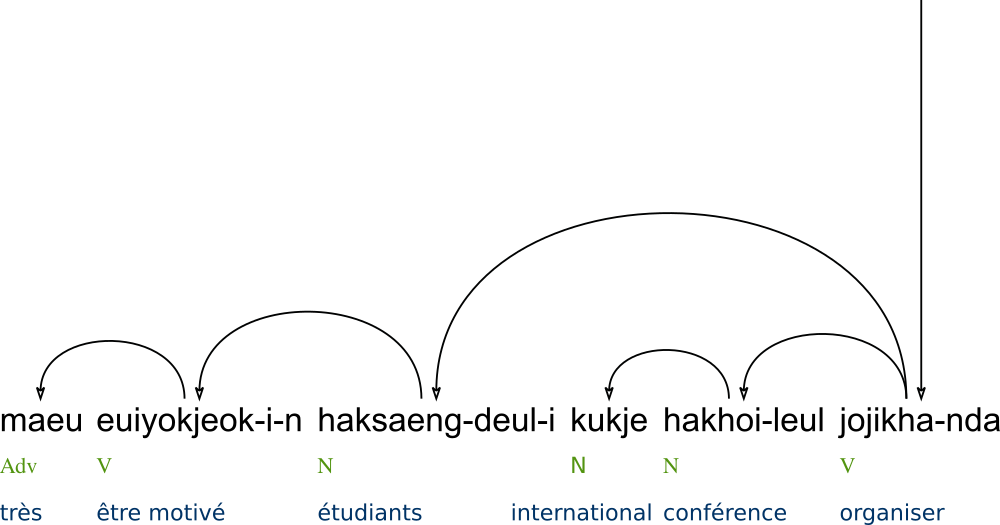
\includegraphics[width=\textwidth]{figures/vol1syntaxe2-img029.png}

    La même phrase traduite en arabe classique (l’arabe du 7\textsuperscript{e} siècle utilisé dans le Coran) possède une structure inversée : tous les gouverneurs se trouvent devant leurs dépendants, y compris le verbe qui se trouve au tout début de la phrase. L’arabe classique est une langue à têtes initiales.
    \ea
    {junazˤimu}  {al+tula:b+u}  {al+mutaħamiss+u:na}  {ʒidan}  {muʔtamar+a+n}  {dawlij+a+n} \\
    V  D+N+NOM  D+Adj+NOM  ADV  N+ACC+D  Adj+ACC\\
    organise.IND.PRES  les étudiants  les enthousiasmés  très  une conférence  internationale

    (IND : indicatif, PRES : prés, NOM:nominatif,ACC:accusatif)
    \z

    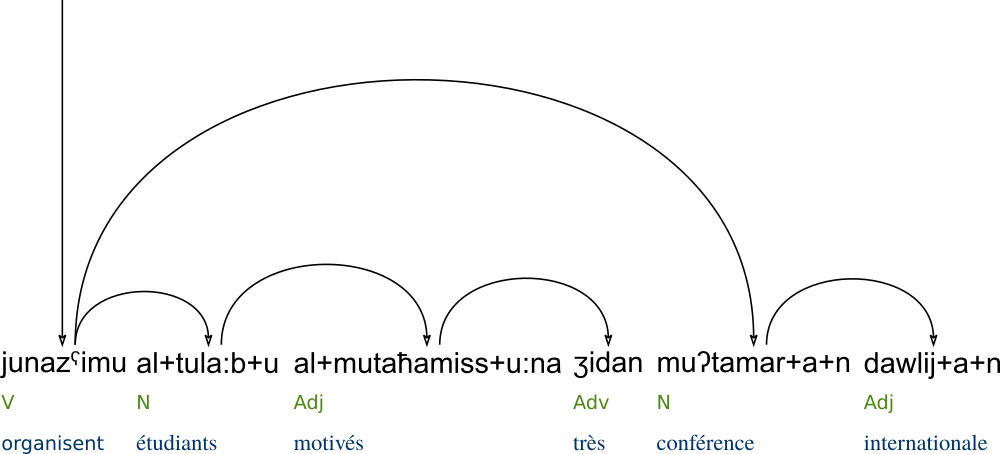
\includegraphics[width=\textwidth]{figures/vol1syntaxe2-img030.png}

    Le français est une langue intermédiaire. L’arbre de dépendance linéarisé de la phrase 1 possède des dépendances dans les deux directions :

    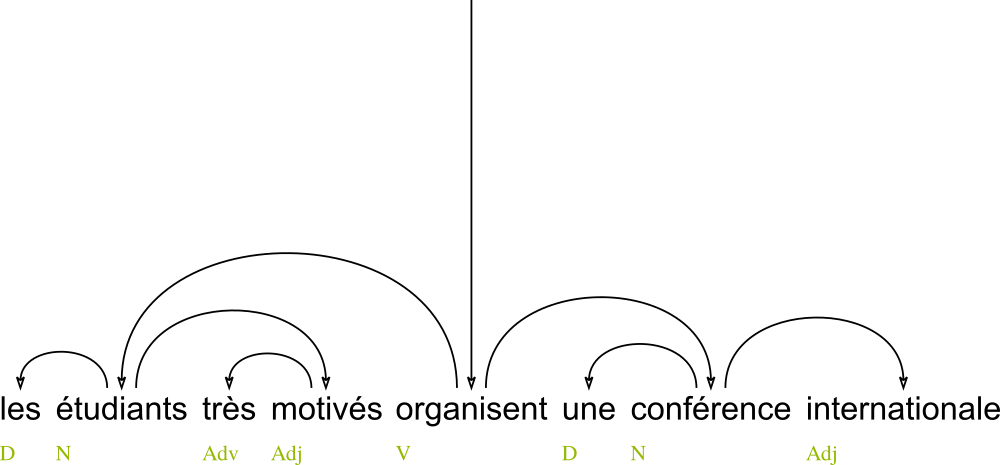
\includegraphics[width=\textwidth]{figures/vol1syntaxe2-img031.png}

    Notez quand même qu’en arabe classique, comme en coréen, il y a des exceptions à la règle du placement de la tête, et les notions de têtes initiales et têtes finales doivent être vue comme des tendances, plutôt que des règles absolues.
}
\globe{Classification des langues selon l’ordre V, S, O}{%\label{sec:3.5.13}
    Depuis les travaux de Greenberg, il est d’usage de classer les langues selon l’ordre dominant entre le verbe (V), son sujet (S) et son objet (O). On considère qu’il y a un \textstyleTermesapprof{ordre dominant} lorsqu’un des six ordres possibles entre V, S et O domine significativement les autres. C’est le cas du français où l’ordre SVO domine largement. La place des S et O pronominaux n’est pas prise en compte, car celle-ci diffère parfois de l’ordre dominant, comme en français où la cliticisation de l’objet (\textit{il} \textbf{\textit{la}} \textit{regarde}) entraine un ordre SOV.

    Le \textit{World Atlas of Language Structures Online} recense actuellement :\todo[inline]{put this in tabular?}

    565 langues SOV, soit 41\%

    488 langues SVO, soit 35\%

    95 langues VSO, soit 7\%

    25 langues VOS, soit 1,8\%

    11 langues OVS, soit 0,8\%

    4 langues OSV, soit 0,3\%

    et 189 langues sans ordre dominant, soit 14\%.

    Comme on le voit, les langues à têtes finales sont beaucoup plus répandues que les langues à têtes initiales et le sujet a nettement tendance à se placer avant l’objet. Il existe une grande proportion de langues SVO, comme le français, où le verbe tend à se placer entre son sujet et son objet, mais l’ordre le plus répandu est quand même l’ordre SOV, celui du coréen. Il est à noter que le classement des langues selon ce principe présuppose que les notions de sujet et d’objet soient pertinentes pour n’importe quelle langue et qu’on soit capable de les identifier. Nous verrons au \chapref{sec:5.2} que la question est loin d’être simple en raison de l’existence de langues dite \textbf{ergatives}. Dans le classement ci-dessus, c’est en fait l’\textbf{agent} et le \textbf{patient}, plus simple à identifier que le sujet et l’objet, qui correspondent à S et O (voir \chapref{sec:5.2}).

    Nous poursuivrons la discussion sur topologie et typologie dans l’\encadref{fig:3.5.23} sur les \textit{Langues dites à ordre libre}, qui n’ont généralement pas d’ordre dominant.
}
\section{Projectivité}\label{sec:3.5.14}

Nous avons déjà évoquée la projectivité à deux reprises au travers du \textbf{test d’insertion} (\sectref{sec:3.2.16} \textit{Tests pour la connexion}) et du \textbf{test de recouvrement} (\sectref{sec:3.3.32} éponyme).

La \textstyleTermes{projectivité} est une propriété qui contraint la linéarisation, c’est-à-dire la correspondance entre un arbre de dépendance et un ordre linéaire. Ce n’est ni une propriété de la structure de dépendance, ni une propriété de la structure d’ordre : c’est une \textbf{propriété} de la structure produit, c’est-à-dire \textbf{de l’arbre} \textbf{de dépendance ordonné}.

Intuitivement, un arbre de dépendance dont tous les mots se placent autour de leur gouverneur est dit projectif. Donnons une première définition formelle de la projectivité :

\begin{styleLivreImportant}
Un arbre de dépendance ordonné est dit \textstyleTermes{projectif} si chacune de ses \textbf{projections} (maximales) est \textbf{continue}, c’est-à-dire forme une portion continue de la chaîne linéaire.
\end{styleLivreImportant}

Le terme \textit{projectivité}, forgé par le mathématicien Yves Lecerf en 1960, renvoie directement à la notion de projection. Dire que la projection de A est continue revient à dire que les dépendants de A se sont placés autour de A et les dépendants de ses dépendants aussi et ainsi de suite et que donc l’ensemble forme un segment continu autour de A.

L’arbre de dépendance ordonné présenté tout à l’heure est projectif :

\begin{figure}
%%[Warning: Draw object ignored]

\caption{\label{fig:}Arbre de dépendance projectif}

\end{figure}

En effet, chaque projection est continue. Par exemple, la projection de \textit{passer}, qui est l’ensemble formé par les mots \textit{passer, Noël, en} et \textit{Laponie}, forme le segment \textit{passer Noël en Laponie}, qui est une portion linéairement continue.

La projectivité entraîne une certaine asymétrie des dépendances. En effet, si A gouverne B, alors la projection de B sera entièrement d’un des deux côtés de A, tandis que la projection de A pourra très bien avoir des parties à gauche et à droite de B.

\begin{figure}
%%[Warning: Draw object ignored]

\caption{\label{fig:}Projections maximales continues}

\end{figure}

C’est sur cette asymétrie qu’est basé le test de recouvrement (\sectref{sec:3.3.32} éponyme).

Il existe une autre caractérisation de la projectivité, qui peut s’observer immédiatement sur une représentation graphique comme celle ci-dessus, où les nœuds sont placés sur une ligne et toutes les dépendances forment des arcs placés du même côté de la ligne.

\begin{styleLivreImportant}
Un arbre de dépendance ordonné est \textstyleTermes{projectif} si et seulement si \textbf{les dépendances ne se coupent pas}.
\end{styleLivreImportant}

Cela concerne également la dépendance verticale qui marque la racine et qui doit être vue comme une dépendance infinie empêchant tout autre dépendance de passée au-dessus de la racine. Autrement dit, les deux configurations suivantes sont exclues d’un arbre de dépendance projectif :

\begin{figure}
%%[Warning: Draw object ignored]

\caption{\label{fig:}Configurations non projectives}

\end{figure}

Donnons un exemple de structure non projective :

\ea
Un petit cordonnier qui voulait aller danser\\
Avait fabriqué de petits souliers.\\
\textbf{Une belle est entrée qui voulait les acheter,}\\
Mais le cordonnier lui a déclaré :\\
«~Ils seront à vous sans qu’il vous coûte un sou,\\
Mais il vous faudra danser avec moi.~»\\
(\textit{Le petit cordonnier}, chanson de Francis Lemarque, 1953)
\z

Le troisième vers de cette chanson a une structure non projective :

\begin{figure}
%%[Warning: Draw object ignored]

\caption{\label{fig:}Arbre de dépendance non projectif}

\end{figure}

Nous avons fait ici une analyse très peu granulaire. Toute analyse plus fine, au niveau du mot par exemple, conservera ces trois dépendances et donc la configuration non projective. (Faire une analyse moins granulaire revient à réduire le graphe. Voir la définition de la réduction dans l’encadré qui suit.)

Comme on le voit sur la figure, la dépendance qui relie \textit{une belle} à la relative \textit{qui voulait les acheter} couvre la racine \textit{est entrée} et coupe donc la dépendance verticale. Il s’en suit que le groupe substantival \textit{une belle qui voulait les acheter} est discontinu.

La projectivité est en partie énoncée par Nicolas Beauzée dans l’article «~Régime~» de l’\textit{Encyclopédie} publié en 1765 (voir la discussion dans l’\encadref{fig:3.3.2} \textit{Historique des notions de dépendance et de tête}) : «~Il ne faut jamais rompre l’unité d’un complément total, pour jeter entre ses parties un autre complément du même mot.~», ce qui reviendrait effectivement à ce que le premier complément soit discontinu. Beauzée note également que les langues à cas peuvent violer la projectivité : «~je crois qu’il est bon de remarquer, que les règles que je viens d’assigner sur l’arrangement de divers compléments, ne peuvent concerner que l’ordre analytique qu’il faut suivre quand on fait la construction d’une phrase, ou l’ordre usuel des langues analogues comme la nôtre. Car pour les langues transpositives, où la terminaison des mots sert à caractériser l’espèce de rapport auquel ils sont employés, la nécessité de marquer ce rapport par la place des mots n’existe plus au même degré.~» La notion de \textit{langue analogue} renvoie ici aux langues ayant un ordre fixe similaire au français (voir l’\encadref{fig:3.5.24} sur l’\textit{Ordre communicativement dirigé}).

\maths{Projectivité et planarité}{%\label{sec:3.5.15}
    La deuxième définition de la projectivité que nous avons donnée (en termes de coupure) est un cas particulier d’une propriété plus générale des graphes que l’on appelle la \textstyleTermesapprof{planarité}. (Pour la notion de graphe voir l’\encadref{fig:1.2.3} sur \textit{Graphe et arbre.})
    \ea
    Un graphe est dit \textstyleTermesapprof{planaire} s’il peut être dessiné dans un plan sans qu’aucunes de ses arêtes ne se coupent.
    \z
    Dans le cas de la projectivité d’un arbre ordonné, on s’intéresse à une propriété qui concerne la relation entre la structure d’arbre et l’ordre linéaire sur les nœuds de l’arbre. Le graphe qui nous intéresse doit donc contenir ces deux structures. Au graphe que forme l’arbre, nous allons ajouter l’ordre linéaire sous la forme d’arêtes entre deux nœuds successifs, ce qui revient à placer les nœuds du graphe sur une ligne dans l’ordre linéaire. Pour prendre totalement en compte la structure hiérarchique de l’arbre, il faut encoder le fait que l’arbre possède un nœud, la racine, qui domine tous les autres. Pour cela, on attache l’arbre par sa racine à un nœud spécial qu’on appelle le nœud à l’infini (noté \textrm{${\infty}$}). Cela revient à placer les nœuds de l’arbre sur un cercle dans l’ordre linéaire avec le nœud à l’infini entre le premier et le dernier nœud. Nous appellerons ce graphe le \textstyleTermesapprof{graphe circulaire} associé à un arbre linéairement ordonné.

    \ea
    %%[Warning: Draw object ignored]
    Graphe circulaire
    \z

    Le graphe circulaire d’un arbre projectif a une propriété un peu plus forte que la planarité : il est planaire extérieur.
    \ea
    Un graphe est dit \textstyleTermesapprof{planaire extérieur} s’il peut être dessiné avec tous ses nœuds accessibles de l’extérieur et sans qu’aucunes de ses arêtes ne se coupent.
    \z
    On peut montrer que pour qu’un graphe soit planaire extérieur, il faut et il suffit qu’il ne puisse pas être réduit à un graphe particulier qu’on appelle K\textsubscript{4}. La \textstyleTermesapprof{réduction} d’un graphe consiste à agréger ensemble des nœuds qui sont liés. C’est une opération importante de notre point de vue, car elle consiste à regarder la structure avec une granularité moins importante (voir la \sectref{sec:3.2.20} sur la \textit{Granularité}). Le graphe K\textsubscript{4} est le graphe complet à 4 nœuds, c’est-à-dire le graphe à 4 nœuds où tous les nœuds sont liés deux à deux. Les deux configurations rejetées par la projectivité sont exactement le graphe K\textsubscript{4}, comme le montre la figure suivante.

    \ea
    %%[Warning: Draw object ignored]
    Equivalence entre K\textsubscript{4} et les configurations non projectives
    \z
}

\loupe{Équivalence des définitions de la projectivité}{%\label{sec:3.5.16}
    On peut donner encore une autre caractérisation de la non-projectivité :

    \ea   Une \textbf{dépendance ordonnée} est \textstyleTermesapprof{non projective} si elle couvre un élément qui n’appartient pas à la projection de la tête de cette dépendance.

    Un \textbf{arbre de dépendance ordonné} est \textstyleTermesapprof{non projectif} si et seulement s’il contient une dépendance non projective.

    Soit T un arbre de dépendance ordonné. On veut montrer l’équivalence des trois propriétés suivantes :

    P1 : T contient une dépendance non projective.

    P2 : T contient un nœud dont la projection est discontinue.

    P3 : T contient deux dépendances qui se coupent.

    Supposons P1. Alors il existe un dépendance \textit{x} \textrm{→} \textit{y} non projective. Cette dépendance couvre un ancêtre \textit{z} de \textit{x}. Par définition, \textit{z} n’est pas dominé par \textit{x} et n’appartient donc pas à la projection X de \textit{x}. Comme z est entre \textit{x} et \textit{y} qui appartiennent à X, X est donc discontinu, d’où P2. Supposons maintenant P2. Soit X un projection discontinue et \textit{z} un élément au milieu de X n’appartenant pas à X. X étant connexe pour la dépendance il existe nécessairement une dépendance \textit{x} \textrm{→} \textit{y} entre deux éléments de X qui relie les parties à gauche et à droite de \textit{z}. Il existe une chaîne de dépendances entre le nœud à l’infini et \textit{z}. Aucun des éléments de cette chaîne ne peut appartenir à X et l’une des dépendances de cette chaîne coupe \textit{x} \textrm{→} \textit{y}, d’où P3. Enfin, si on a P3, nécessairement l’une des deux dépendances qui se coupent est non projective et on à P1. Nous avons montré l’équivalence des trois propriétés.
    \z
}
\loupe{Flux de dépendances}{%\label{sec:3.5.17}
    Le \textstyleTermesapprof{flux de dépendances} en un point de l’ordre linéaire est l’\textbf{ensemble des dépendances} qui \textbf{relient} un \textbf{nœud} \textbf{à gauche} à un \textbf{nœud} \textbf{à droite} de ce point. Le flux de dépendance est défini pour un arbre linéairement ordonné. Ce qu’on appelle un point de l’ordre linéaire est une position sur la ligne que forment les mots lorsqu’on les aligne de gauche à droite dans l’ordre linéaire. On s’intéresse généralement au flux entre deux mots successifs, c’est-à-dire au \textbf{flux inter-mot}, mais on peut aussi regarder le flux au-dessus d’un syntaxème donné.

    \ea
    %%[Warning: Draw object ignored]
    %%[Warning: Draw object ignored]
    %%[Warning: Draw object ignored]
    %%[Warning: Draw object ignored]
    %%[Warning: Draw object ignored]
    %%[Warning: Draw object ignored]
    %%[Warning: Draw object ignored]
    %%[Warning: Draw object ignored]
    %%[Warning: Draw object ignored]

    %%[Warning: Draw object ignored]
    Flux inter-mot
    \z

    Dans notre figure, le flux en un point de la phrase est l’ensemble des dépendances qui coupent le trait vertical en ce point. Le flux entre deux phrases est vide (à moins que l’on considère aussi des dépendances entre phrases). En toute position inter-mot de la phrase, le flux contient au moins une dépendance. Le flux entre \textit{de} et \textit{gens} ou entre \textit{passer} et \textit{Noël} contient deux dépendances.

    La première propriété du flux est qu’il semble être naturellement \textbf{borné}, c’est-à-dire que le nombre de dépendances qui appartiennent simultanément au flux en n’importe quel point de la chaîne parlée ne dépasse jamais une certaine valeur. De ce point de vue, il faut distinguer deux types de configurations : les dépendances en bouquet, qui partagent une extrémité commune, et les dépendances disjointes. Les dépendances disjointes correspondent à des enchâssements centrés (angl. \textit{center embeddings}) de syntagmes, qui s’avère beaucoup plus coûteux pour le traitement que la présence de plusieurs dépendants sur un même élément.


    \ea
    %%[Warning: Draw object ignored]

        \textbf{Dépendances en bouquet}     \textbf{Dépendances disjointes}
    \z

    Les études faites sur des corpus annotés dans plus de 70 langues montrent que le flux n’a jamais plus de 6 dépendances disjointes et que ce nombre n’est quasiment jamais atteint. Plusieurs expériences en psychologie ont montré que le nombre de paramètres que l’on peut conserver simultanément dans sa \textbf{mémoire immédiate} dépasse rarement 7 (voir le fameux article du psychologue George Miller de 1956 intitulé \textit{The magical number seven, plus or minus two: Some limits on our capacity for processing information}). Par exemple, si vous montrez pendant une fraction de seconde à une personne un écran noir avec 5 ou 6 points blancs disposés aléatoirement, elle devrait être capable de vous dire précisément le nombre de points qui sont apparus à l’écran. Mais si vous faites la même expérience avec 8 ou 9 points, cela devient beaucoup plus difficile. On peut penser que la même contrainte agit sur le flux de dépendances et rend compte du fait que nous ne sommes pas capable de traiter simultanément plus de 6 dépendances disjointes lorsque nous écoutons une phrase et l’analysons au fur et à mesure de son écoute. La même contrainte agit lorsque nous produisons un énoncé et que nous devons gérer le flux de dépendances pour assurer la cohésion de notre propos.

    Nous allons maintenant préciser les liens entre le flux de dépendances et l’analyse d’un énoncé. Pour un arbre projectif, le flux est naturellement ordonné. Deux dépendances sont dites \textstyleTermesapprof{concomitantes} si elles appartiennent ensemble au flux à un moment donné. Lorsque l’arbre est projectif, deux dépendances concomitantes vérifient toujours la propriété suivante : l’un des dépendances couvre entièrement l’autre. On peut donc \textbf{ordonner le flux} de la plus petite dépendance à la plus grande et voir l’ensemble des dépendances à traiter à un moment donné comme une \textstyleTermesapprof{pile de dépendances} (ici pile fait référence à une pile d’assiettes). Cette idée a été exploitée pour le calcul automatique d’un arbre dépendance. Nous considérons que l’analyse d’une phrase se fait \textbf{incrémentalement}, c’est-à-dire en traitant les mots les uns après les autres dans leur ordre linéaire. À chaque mot traité, de nouvelles connexions sont effectuées et le flux de dépendances est mis à jour. Autrement dit, traiter un nouveau mot consiste à chercher ses connexions à gauche (c’est-à-dire parmi les mots déjà traités) et à introduire dans le flux ses connexions potentielles à droite. Dans l’absolu, le nombre d’information à traiter devrait grossir au fur et à mesure que de nouveaux mots sont considérés. C’est là qu’intervient la projectivité : en raison des contraintes de projectivité, les connexions potentielles qui figurent dans le flux sont ordonnées. Ce sont les dernières connexions entrées dans le flux qui doivent être traitées les premières, d’où l’idée de traiter l’ensemble des dépendances comme une pile d’assiettes : la dernière dépendance potentielle entrée dans le flux est posée sur le haut de la pile. Lorsqu’un nouveau mot est traité, seul le haut de la pile est considéré et le mot courant peut ou non accepter la connexion potentielle qui s’y trouve. S’il veut accéder à une autre connexion potentielle, il faut que la connexion potentielle qui est sur le dessus de la pile soit supprimable et supprimée. La procédure d’analyse que nous venons de décrire est appelée l’\textstyleTermesapprof{analyse en flux}.

    On peut encore noter que les positions inter-mot et les dépendances se correspondent une à une. En effet, un arbre de dépendance à \textit{n} nœuds contient \textit{n}–1 dépendances et, s’il est linéairement ordonné, il possède \textit{n}–1 positions inter-mot. En tout point de l’ordre linéaire où le fux est projectif, on peut identifier une plus petite dépendance couvrant ce point que l’on appelle la \textstyleTermesapprof{voûte} et associer ainsi cette position inter-mot à cette dépendance. Il est intéressant de noter que cette dépendance donne une information importante sur la position inter-mot en tant que frontière. Reprenons l’exemple au début de cet encadré. La voûte de la position inter-mot entre \textit{gens} et \textit{aimeraient} est la relation sujet entre \textit{aimeraient} et \textit{beaucoup~}; la position est donc la frontière droite du sujet.
}
\section{Linéarisation projective}\label{sec:3.5.18}

Nous allons maintenant étudier l’ordre des mots, c’est-à-dire la correspondance entre la structure de dépendance syntaxique et l’ordre linéaire, en nous plaçant dans la situation où nous voudrions ordonner un arbre de dépendance d’une langue donnée. Nous commençons par le cas, plus simple, où la linéarisation de l’arbre de dépendance donne un arbre ordonné projectif.

La projectivité contraint fortement les linéarisations possibles d’un arbre de dépendance. Elle contraint chaque nœud de l’arbre de dépendance syntaxique à rester proche de son gouverneur et donc à \textbf{se placer par rapport à son gouverneur et à ses co-dépendants} (c’est-à-dire les éléments qui dépendent du même nœud que lui).

Nous allons commencer par montrer comment le placement par rapport au gouverneur combiné avec la projectivité permet de spécifier un certain nombre d’ordres linéaires possibles, puis nous étudierons le placement par rapport aux co-dépendants dans les sections suivantes. Nous terminerons ce chapitre en étudiant la linéarisation non projective, pour laquelle le placement ne se fait plus par rapport au gouverneur.

Reprenons notre exemple favori :

\ea
{Beaucoup de gens aimeraient passer Noël en Laponie}.
\z

Indiquons pour chaque type de mot comment il se place par rapport à son gouverneur en français :

\begin{itemize}
\item le sujet précède le verbe dont il dépend ;
\item l’objet suit le verbe dont il dépend ;
\item les compléments propositionnels se placent après leur gouverneur ;
\item le complément d’une préposition se place après celle-ci.
\end{itemize}

De telles règles sont appelées des \textstyleTermes{règles de précédence linéaire}. Elles peuvent être énoncées en termes de dépendances ou de constituants, peu importe la granularité de la combinaison que nous considérons pour un type de connexion donnée.

En projetant ces règles sur l’arbre de dépendance de la phrase, on obtient la structure suivante où est indiqué, pour chaque dépendance, si le dépendant se place avant (<) ou après (>) le gouverneur :

\begin{figure}
%%[Warning: Draw object ignored]

\caption{\label{fig:Arbre de dépendance avec spécifications d’ordre}}

\end{figure}

Pour ordonner linéairement les nœuds de l’arbre, on peut par exemple parcourir l’arbre à partir de sa racine en plaçant les nœuds au fur et à mesure. On place donc d’abord le verbe \textit{aimeraient}, puis ses deux dépendants, l’un à gauche (\textit{beaucoup}) et l’autre à droite (\textit{passer}) :
\ea
    {beaucoup aimeraient passer}
\z
On place ensuite le dépendant de \textit{beaucoup} à sa droite. La projectivité bloque une linéarisation telle *\textit{beaucoup aimeraient} \textbf{\textit{de gens}} \textit{passer}, qui respecte pourtant les règles de placement dépendant-gouverneur. En effet, \textit{de gens} doit se passer après \textit{beaucoup}, mais il ne peut pas aller au-delà de \textit{aimeraient,} car \textit{aimeraient} n’est pas dans la projection de \textit{beaucoup}. On a donc nécessairement :
\ea
    {beaucoup de gens aimeraient passer}
\z
On place ensuite les dépendants de \textit{passer} à sa droite. À défaut de règles ordonnant les co-dépendants, on obtient deux ordres possibles : notre phrase de départ et la phrase \textit{Beaucoup de gens aimeraient passer en Laponie Noël} (sur laquelle nous reviendrons dans l’\encadref{fig:3.5.21} sur les \textit{Préférences dans l’ordre}).

Comme on le voit, la projectivité et des règles indiquant l’ordre dépendant-gouverneur permettent de contrôler de manière assez précise l’ordre des mots. Nous allons voir comment compléter ces règles de base.

\section{Linéarisation des co-dépendants}\label{sec:3.5.19}

Dès qu’un nœud a plus de deux dépendants, l’un des dépendants ne pourra pas être accolé à son gouverneur. Considérons l’exemple suivant :
\ea
{Le petit garçon ne lui prêtera pas son autre gros ballon}.
\z
Voici son arbre de dépendance (où nous indiquons les seules fonctions pertinentes pour la suite de discussion, à savoir \textit{sujet} et \textit{objet}) :

\begin{figure}
%%[Warning: Draw object ignored]

\caption{\label{fig:}Arbre de dépendance}

\end{figure}

 (Remarque : nous décidons dans cet arbre de prendre le nom comme tête du groupe substantival. Comme nous l’avons expliqué dans le \chapref{sec:3.3}, le déterminant comme le nom ont des propriétés de tête. Le choix du déterminant comme tête poserait encore moins de problème pour la linéarisation.)

L’ordre dépendant-gouverneur n’est pas suffisant pour contraindre correctement les ordres possibles : il est également nécessaire d’\textbf{ordonner entre eux les co-dépendants} \textbf{d’un} \textbf{même nœud} qui se placent du même côté de leur gouverneur commun.

On peut envisager deux façons d’exprimer les règles d’ordre entre co-dépendants.

Une première méthode consiste à considérer des règles d’\textbf{ordre des co-dépendants} \textbf{deux à deux} (ce serait à nouveau des \textbf{règles de précédence linéaire}). Par exemple, pour obtenir l’ordre \textit{le petit garçon} et bannir *\textit{petit le garçon}, on indiquera que~le déterminant se place devant les adjectifs qui dépendent du même nom. Si l’on regarde maintenant, l’ordre des dépendants à gauche du verbe \textit{prêtera}, on indiquera que le sujet se place avant les clitiques et que le clitique \textit{ne} précède toujours les clitiques datifs (comme \textit{lui}). Si on regarde plus précisément l’ordre des clitiques préverbaux du français, on voit qu’on a toujours \textit{je} < \textit{ne} < \textit{me} < \textit{le} < \textit{lui} < \textit{y} < \textit{en} < verbe : \textit{il me le donne, je le lui donne, il n’y en a pas,} etc. Comme l’ordre entre les clitiques est total, il est plus économique de donner directement l’ordre complet comme nous l’avons fait, que de donner les ordres des co-dépendants deux à deux (étant donné qu’il y a 8 éléments à ordonner, cela nous fait 7${\times}$8/2, soit 28 couples à ordonner).

La deuxième méthode pour ordonner les co-dépendants consiste donc à donner d’un coup l’ensemble des règles d’ordre concernant un nœud et ses dépendants. Cela peut être fait en considérant que chaque nœud de l’arbre de dépendance ouvre une \textbf{boîte ordonnée} avec des positions prévues pour les différents dépendants selon leur nature et leur fonction. Nous appellerons une telle boîte un \textstyleTermes{gabarit topologique} et chacune des cases de la boîte un \textstyleTermes{champ topologique}.

Voici le gabarit qu’ouvre un verbe à l’indicatif en français :

\begin{table}
\caption{\label{tab:}}
\begin{tabularx}{\textwidth}{XXXXXXXXXXXXXX}
\lsptoprule
\multicolumn{14}{c}{{\bfseries Domaine verbal}}\\
\midrule
\multicolumn{1}{c}{ch-pré-noyau} & \multicolumn{1}{c}{ch-initial} & \multicolumn{1}{c}{ch-cl-sujet} & \multicolumn{1}{c}{ch-cl-ne} & \multicolumn{1}{c}{ch-cl-se} & \multicolumn{1}{c}{ch-cl-le} & \multicolumn{1}{c}{ch-cl-lui} & \multicolumn{1}{c}{ch-cl-y} & \multicolumn{1}{c}{ch-cl-en} & \multicolumn{1}{c}{ch-verbe} & \multicolumn{1}{c}{ch-adv} & \multicolumn{1}{c}{ch-vb-sub} & \multicolumn{1}{c}{ch-final} & ch-post-noyau\\
\lspbottomrule
\end{tabularx}
\end{table}

Ce gabarit contient 7 champs préverbaux pour des clitiques (les champs ch-cl-X), un champ initial dont nous avons parlé au début de ce chapitre et qui accueille en général le sujet, un champ final qui accueille les compléments du verbe, un champ pour un verbe subordonné (notamment pour le participe des formes verbales complexes comme \textit{a dormi}) précédé d’un champ adverbial (pour la négation \textit{pas} entre autres) et des champs pré-noyau et post-noyau qui accueillent les éléments détachés à gauche et à droite (voir partie 6 sur la macrosyntaxe). Les éléments qui viennent se placer dans le gabarit ouvert par le verbe vont former avec lui un constituant, dit \textstyleTermes{constituant topologique}, que nous appelons le \textstyleTermes{domaine verbal}.

Les champs possèdent des \textstyleTermes{contraintes d’occupation} diverses. Certains champs ne peuvent recevoir qu’un seul élément, comme les champs clitiques ou le champ initial. D’autres peuvent recevoir plusieurs éléments comme le champ final où les champs pré- et post-noyau. Certains champs sont liés comme le champ initial et le champ clitique sujet qui ne peuvent être remplis tous les deux. (Voir aussi l’\encadref{fig:3.5.20} qui suit).

La méthode avec gabarit a l’avantage que les règles d’ordre reste finalement essentiellement des règles d’ordre d’un nœud par rapport à son gouverneur. Mais au lieu d’indiquer simplement si le dépendant va à gauche ou à droite de son dépendant (< ou >), \textbf{une règle d’ordre} \textbf{indique dans quel champ du gabarit ouvert par son gouverneur va chaque dépendant}. Par exemple :

\begin{itemize}
\item Le sujet non clitique peut aller dans le champ initial ; les sujets clitiques ne vont pas dans le champ initial, car à la différence des sujets non-clitiques, ils ne peuvent pas être séparés du verbe par un insertion : \textit{Félix, je pense, prêtera son ballon} vs. *\textit{Il, je pense, prêtera son ballon}.
\item Un pronom clitique de 1\textsuperscript{ère} ou 2\textsuperscript{ème} personne va dans le champ clitique ch-cl-se (\textit{il ne} \textbf{\textit{vous}} \textit{le donnera pas}).
\item Un complément non clitique peut aller dans le champ final.
\end{itemize}

Et ainsi de suite.

\loupe{Un cas d’exclusion étrange}{%\label{sec:3.5.20}

    Nous avons, dans le début de ce chapitre, considéré que l’exclusion mutuelle pouvait découler soit de l’occupation d’une même position syntaxique (*\textbf{\textit{Qui}} \textit{Pierre} \textbf{\textit{la}} \textit{regarde-t-il} ?), soit d’une même position topologique (*\textit{Leider Peter popelt schon wieder in seiner Nase}, voir l’\encadref{fig:3.5.5} sur \textit{Le cas des langues V2}). Il existe néanmoins des cas d’exclusion qui ne relèvent ni d’une situation, ni de l’autre. Tel est le cas des clitiques \textit{te} et \textit{lui} (et des clitiques qui appartiennent aux mêmes paradigmes). Voici les données :
    \ea
    {Il te/la vendra au roi.}  [ici \textit{te} ou \textit{la} sont objets direct]
    \z
    \ea
    {Il me/lui vendra sa fille.}  [ici \textit{me} ou \textit{lui} sont objet indirect]
    \z
    \ea
    {Il me la vendra.}
    \z
\ea{
    Il la lui vendra.
    }
    \z
    \ea
    {*Il me te vendra}    (vs. \textit{Il te vendra à moi}.)
    \z
    \ea
    {*Il te lui vendra.}    (vs. \textit{Il te vendra à lui}.)
    \z

    L’inacceptabilité des deux derniers exemples ne vient pas d’une exclusion syntaxique, puisque \textit{te} et \textit{me}/\textit{lui} n’occupe pas la même position syntaxique (l’un est objet direct et l’autre objet indirect). Or il ne semble pas s’agir non plus d’une exclusion topologique, puisque \textit{me} objet indirect et \textit{lui} occupent des positions topologiques différentes (l’un se place avant \textit{la} et l’autre après).

    Tout se passe comme si \textit{te} ou \textit{me} (en tant qu’objet direct) bloquait les trois positions topologiques à la fois (celles de \textit{te/me} objet indirect, \textit{le} et \textit{lui}).

    \begin{tabularx}{\textwidth}{XXXXXXXX}
    \lsptoprule
    \multicolumn{1}{c}{{\sffamily\itshape il}} & {\sffamily\itshape ne} & \multicolumn{1}{c}{{\sffamily \textit{me} (indirect)}} & \multicolumn{1}{c}{{\sffamily\itshape le}} & {\sffamily\itshape lui} & \multicolumn{1}{c}{{\sffamily\itshape y}} & \multicolumn{1}{c}{{\sffamily\itshape en}} & \multicolumn{1}{c}{{\sffamily verbe}}\\
    \multicolumn{2}{c}{} & \multicolumn{3}{c}{{\sffamily \textit{me} (direct)}} & \multicolumn{3}{c}{}\\
    \hhline{~~---~~~}
    \lspbottomrule
    \end{tabularx}

    Le fait que cette exclusion ne puisse être clairement imputée ni à des règles syntaxiques, ni à des règles topologiques est un des arguments avancés pour considérer que la grammaire des clitiques préverbaux du français relèvent aujourd’hui de la conjugaison du verbe, laquelle, on le sait, est beaucoup plus irrégulière que la microsyntaxe. Nous considérons pour notre part qu’il s’agit effectivement de nanosyntaxe, sans considérer pour autant qu’il s’agit de flexion (voir \chapref{sec:4.2}).
}
\section{Préférences dans l’ordre}\label{sec:3.5.21}

La méthode des gabarits permet de rendre compte des contraintes d’ordre rigides, comme celles des clitiques préverbaux : ici chaque élément occupe une position précise et toute variation est agrammaticale. Mais il arrive plus couramment que l’ordre entre deux co-dépendants soit libre. Tel est le cas des compléments du verbe en français. Comme le montre les exemples suivants, l’objet direct et l’objet indirect peuvent se placer assez librement l’un par rapport à l’autre :
\ea
    {Félix a prêté} un livre \textbf{{à sa sœur.}}
\z
\ea
    {Félix a prêté} \textbf{{à sa sœur}} un livre qu’il aime bien.
\z
Nous modélisons cela en indiquant que les deux compléments vont dans le même champ (que nous avons appelé le champ final). Il y a néanmoins des préférences entre les deux ordres dont la méthode des gabarits ne rend pas compte. Ces préférences dépendent de différents paramètres, les deux principaux étant le poids et la saillance communicative.

Le \textstyleTermes{poids} d’un constituant correspond en fait à sa taille du point de vue phonologique, c’est-à-dire à son nombre de syllabes. Un constituant qui possède un grand nombre de syllabes est dit \textstyleTermes{lourd}, alors qu’un petit constituant, généralement monosyllabique, est dit \textstyleTermes{léger}. Plus un constituant est lourd, plus il a tendance à être éloigné de son gouverneur. Par exemple, en linéarisant l’arbre de dépendance de notre exemple favori, nous avons obtenu la phrase \textit{Beaucoup de gens aimeraient passer en Laponie Noël}, qui apparaît moins naturelle que la phrase d’origine. On l’améliore nettement en alourdissant le poids de l’objet direct :
\ea
    {Beaucoup de gens aimeraient passer en Laponie les fêtes de fin d’année}.
\z
Il est possible que joue ici une contrainte prosodique. Comme nous l’avons déjà vu dans la \sectref{sec:3.2.11} sur l’\textit{Unité syntaxique autonomisable}, les constituants prosodiques sont des unités syntaxiques, c’est-à-dire des unités connexes pour la dépendance. Considérons l’exemple suivant, \textit{là} est séparé de son gouverneur \textit{passer} par un co-dépendant, \textit{les fêtes de fin d’année~}:

\ea
{Beaucoup de gens aimeraient passer les fêtes de fin d’année} \textbf{{là}}.
\z
Un constituant qui est séparé de son gouverneur par un co-dépendant ne peut former d’unité syntaxique avec son voisin sans inclure leur gouverneur commun. Si un constituant léger n’est pas à côté de son gouverneur, il est donc contraint soit à former une petite unité prosodique à lui-seul, soit au contraire à former une grande unité prosodique avec ses voisins qui devra inclure leur gouverneur commun \textit{passer}. Dans les deux cas, cela nuit à l’équilibre prosodique de l’énoncé. On préférera généralement l’ordre inverse (\textit{passer là les fêtes de fin d’année}) beaucoup moins contraignant.

La \textstyleTermes{saillance communicative} d’un constituant est l’importance que joue ce constituant du point de vue de l’information à communiquer. Par exemple, si on parle de la Laponie et que c’est bien l’information \textit{Noël} que l’on souhaite mettre en avant, il devient plus naturel de produire la phrase \textit{Beaucoup de gens aimeraient passer en Laponie Noël}. Il y a par ailleurs une corrélation entre saillance et poids, puisqu’un des moyens de rendre saillante une information est de lui donner du poids.

Ce phénomène de \textstyleTermes{rejet des constituants lourds} (appelé par les générativistes \textit{heavy shift}) a été remarqué il y a bien longtemps. Ainsi, Claude Buffier, dans sa \textit{Grammaire françoise sur un plan nouveau} de 1709 disait (p. 313) :

\begin{quote}
    «~Les régimes [= compléments] doivent être le plus près qu’il se peut du mot régissant ; ce qui feroit pas si l’on mettoit d’abord le plus long qui éloigneroit trop le plus court.~»
\end{quote}
Nicolas Beauzée développait cette remarque dans l’entrée «~Régime~» de l’\textit{Encyclopédie} en 1765 (celle-là même où il définit le complément) :
\begin{quote}
    «~De plusieurs \textit{compléments} qui tombent sur le même mot, il faut mettre le plus court le premier après le mot \textit{complété ;} ensuite le plus court de ceux qui restent, et ainsi de suite jusqu’au plus long de tous qui doit être le dernier. […] il importe à la netteté de l’expression, \textit{\textit{cujus summa laus perspicuitas}}, de n’éloigner d’un mot, que le moins qu’il est possible, ce qui lui sert de \textit{complément}. Cependant quand plusieurs \textit{compléments} concourent à la détermination d’un même terme, ils ne peuvent pas tous le suivre immédiatement ; et il ne reste plus qu’à en rapprocher le plus qu’il est possible celui qu’on est forcé d’en tenir éloigné : c’est ce que l’on fait en mettant d’abord le premier celui qui a le plus de brièveté, et réservant pour la fin celui qui a le plus d’étendue.~»
\end{quote}
Mais c’est à Henri Weil (\citeyear{Weil1844}, p. 97-102), critiquant Beauzée (critique qui s’appliquerait à bien des analyses depuis) qu’on doit, à notre avis, l’analyse la plus pertinente :
\begin{quote}
    «~De plusieurs compléments qui tombent sur le même mot, donnez la forme la plus concise à celui qui suit immédiatement le mot complété et, à mesure que vous avancez, donnez aux compléments une expression plus développée et plus étendue.~»
\end{quote}
En d’autres termes, ce n’est pas parce qu’un complément est lourd qu’il doit être placé loin de son gouverneur, mais c’est parce qu’il est loin de son gouverneur qu’il doit être lourd. Weil conclut par ces mots :
\begin{quote}
    «~La parole est au service de la pensée, et non pas la pensée au service de la parole.~»
\end{quote}
\loupe{Contraintes de poids}{%\label{sec:3.5.22}
    Une façon de rendre contre des préférences dans l’ordre des co-dépendants est de voir certaines dépendances comme pourvu d’\textstyleTermesapprof{élasticité}. On peut ainsi distinguer des dépendances rigides comme la dépendance entre un clitique préverbal et le verbe dont la «~longueur~» est fixe et des dépendances beaucoup plus souples comme celle entre un complément non clitique et le verbe. On peut alors se représenter les \textstyleTermesapprof{contraintes de poids} des constituants lourds comme véritablement exercées par les forces gravitationnelles : les différents dépendants sont comme suspendus à leur gouverneur et plus ceux-ci sont lourds, plus ils allongent la dépendance qui les relie à leur gouverneur et s’en trouvent éloignés. Considérons la phrase :
    \ea
    {Le professeur propose aujourd’hui à ses élèves un exercice sur l’ordre des mots.}
    \z
    Voici comment s’étirent, en fonction de leur poids, les différentes dépendance entre le verbe \textit{propose} et ses compléments :

    \ea
    %%[Warning: Draw object ignored]
    \z

    La position finale d’un dépendant se trouve alors déterminée par la «~longueur~» initiale de la dépendance (déterminée par la fonction et la nature du dépendant comme dans le modèle avec gabarit), l’élasticité de cette dépendance et différents paramètres comme le poids ou la saillance.
}
\globe{Les langues dites à ordre libre}{%\label{sec:3.5.23}
    Une langue est dite \textstyleTermesapprof{à ordre libre} quand une tête et ses dépendants (et notamment le verbe, son sujet et son objet) peuvent être dans n’importe quel ordre. Lorsque, au contraire, un seul ordre est possible, on dit que la langue est \textstyleTermesapprof{à ordre rigide}. Il existe entre les deux toute une gamme de langues à ordre plus ou moins libre ou plus ou moins rigide.

    L’ordre des mots en français est particulièrement rigide, même s’il l’est un peu moins qu’en anglais. L’allemand a un ordre plus libre que le français. Par exemple, on peut traduire \textit{Marie poursuit Pierre} par \textit{die Marie verfolgt den Pierre} ou bien par \textit{den Pierre verfolgt die Marie.} Les deux phrases ont le même \textbf{contenu informationnel} (voir chapitres\todo[inline]{sg?} \ref{sec:1.2}), c’est-à-dire qu’elles décrivent le même état du monde : chaque fois c’est Marie qui poursuit Pierre et pas l’inverse. Le repérage des dépendants du verbe est effectué en allemand grâce à un \textstyleTermesapprof{système casuel}, c’est-à-dire des marques sur certains mots du syntagme substantival qui n’ont pas d’autre rôle que justement d’indiquer la relation qu’entretient le syntagme avec le verbe. (Voir la notion de \textit{cas} au \chapref{sec:4.2}.) Ce sont avant tout les déterminants qui portent l’information casuelle en allemand. Dans notre exemple, le fait que \textit{den Pierre} soit l’objet est marqué par le cas accusatif du déterminant masculin singulier \textit{den} (qui s’oppose au déterminant au nominatif \textit{der}).

    L’ordre des mots en allemand n’est cependant pas libre au sens où seuls deux des six ordres possibles entre les trois mots correspondant à \textit{Marie}, \textit{Pierre} et \textit{poursuit} sont possibles pour une phrase déclarative. Il existe d’autres langues, comme les langues slaves ou le grec moderne, où les six ordres des trois mots sont acceptables et désignent le même état du monde. Voici un exemple du russe :
\ea
    \ea
    Vanya prigotovil malinu\\
    \glt  ‘Vanya a préparé les framboises’ \\
    \glt  ‘Ce que Vanya a préparé, c’est les framboises’

    \ex Prigotovil Vanya malinu
    \glt ‘Ce qu’a préparé Vanya, c’est les framboises’

    \ex Malinu prigotovil Vanya
    \glt  ‘C’est les framboises qu’a préparé Vanya’

    \ex Malinu Vanya prigotovil
    \glt   ‘C’est les framboises que Vanya a préparé’

    \ex Prigotovil malinu Vanya
    \glt ‘Ce qu’il a préparé, c’est les framboises, Vanya’

    \ex Vanya malinu prigotovil
    \glt  ‘Vanya, c’est les framboises qu’il a préparé’
\z
\z
    Nous avons donné ici les traductions en français lorsque ces phrases répondent à une question sous-jacente telle \textit{Qu’a préparé Vanya} ?, c’est-à-dire que \textit{malinu} ‘les framboises’ est le \textstyleTermesapprof{rhème} (ce qu’on dit), tandis que \textit{Vanya prigotovil} ‘Vanya a préparé’ est le \textstyleTermesapprof{thème} (ce dont on parle).

    Si on regarde les traductions françaises, on remarque que les variations entre ces phrases sont constituées de constructions qui servent à mettre en avant un élément de la phrase. La construction avec «~\textit{C’est … que}~», appelée \textstyleTermesapprof{clivée} (voir le test de clivage en 3.4.9) est utilisée dans les traductions des phrases 3, 4 et 6 pour mettre en valeur un élément rhématique non verbal~(ici \textit{les framboises}). Très similaire est la \textstyleTermesapprof{pseudo-clivée} «~Ce que …, c’est … » utilisée pour les traductions des phrases 1, 2 et 5. À ces constructions s’opposent la \textstyleTermesapprof{dislocation gauche}, qui sert à distinguer un élément thématique, comme \textit{Vanya} dans la traduction de la phrase 6. Similairement, on peut aussi disloquer un élément thématique à droite comme \textit{Vanya} dans la traduction de phrase 5. Les six ordres en russe s’accompagnent évidemment de légères différences de sens, relevant de la structure communicative (voir l’encadré suivant), similaires à celles que montrent leurs traductions en français. Il n’en reste pas moins que les six ordres sont possibles.

    Notez ensuite que, abstraction faite des mots fonctionnels des différentes constructions, dans les deux langues considérées, le russe et le français, les trois mots lexicaux se trouvent toujours dans le même ordre. À cela s’ajoute que les principaux prosodèmes, qui constituent l’intonation de la phrase se ressemblent pour chacun des ordres possibles. La phrase 2 par exemple, a une courbe intonative que l’on peut schématiser comme suit, avec une intonation montante sur le thème (\textit{prigotovil Vanya}) et une intonation descendante sur le rhème (\textit{malinu}).

    \ea
    %%[Warning: Draw object ignored]
    %%[Warning: Draw object ignored]

        {Prigotovil}   {Vanya}   {malinu}

    ‘Ce que prépare  Vanya,  c’est les framboises’
    \z

    Il paraît évident qu’il existe une relation entre l’existence d’un système casuel et la liberté dans le placement des arguments verbaux : il serait en effet redondant d’obliger un objet à la fois à porter un marqueur casuel d’accusatif \textit{et} à occuper une place fixe. L’inverse, par contre, n’est pas tout à fait vrai. Une langue sans système casuel n’est pas forcément très restrictive quant à l’ordre des arguments verbaux. Un bel exemple est le bahasa, la principale langue parlée en Malaisie et en Indonésie, aussi appelée le malais ou l’indonésien selon ses variantes dialectales. Cette langue ne connait pas de flexion casuelle et pourtant elle permet une plus grande liberté de mots que d’autres langues sans flexion. Si l’ordre dominant est l’ordre SVO comme dans la phrase a, il est possible de postposer le sujet comme en b et d’antéposer l’objet comme en c.
    \ea
    \ea
    \gll Ali baca buku itu.\\
    Ali lire    livre  ce\\
    \glt  ‘Ali lit ce livre’
    \ex
    \gll baca buku itu Ali.\\
    lire    livre  ce Ali\\
    \glt  ‘Il lit ce livre, Ali’
    \ex
    \gll buku itu Ali baca.\\
        livre ce Ali lire    \\
    \glt  ‘Ce livre, Ali le lit’
    \z
    \z

    On peut comparer cette situation avec celle que propose le français à l’oral, où, avec les dislocations gauches et droites, les six ordres sont possibles sans qu’il n’y ait aucune marque casuelle :

    \begin{enumerate}
    \item {Ali, ce livre, il le lit.}
    \item {Ali, il le lit, ce livre.}
    \item {Il le lit, Ali, ce livre.}
    \item {Ce livre, Ali, il le lit.}
    \item {Ce livre, il le lit, Ali.}
    \item {Il le lit, ce livre, Ali.}
    \end{enumerate}
}
\globe{Ordre communicativement dirigé}{%\label{sec:3.5.24}
    Les \textbf{langues à ordre rigide} (voir l’encadré qui précède) sont généralement des langues où la position topologique est fortement déterminée par la fonction syntaxique et la catégorie syntaxique. Ainsi, en français, un objet direct doit nécessairement être après le verbe, à moins que ce soit un clitique, un pronom relatif ou un pronom interrogatif. Autrement dit, en français, l’ordre linéaire est utilisé pour marqué la fonction syntaxique et permettre le repérage de l’objet par rapport au sujet. Nous dirons que de telles langues ont un \textstyleTermesapprof{ordre syntaxiquement dirigé}.

    A l’inverse dans \textbf{les langues à ordre libre}, la fonction syntaxique joue peu de rôle, puisque, quelle que soit la fonction syntaxique, tous les ordres sont possibles. Il ne faut pas croire pour autant que l’ordre dans ces langues soit non motivé et que tous les ordres se valent. Il existe un \textbf{principe d’économie} qui veut que les langues cherchent à en dire le maximum avec le minimum de moyens : il n’est donc même pas imaginable qu’un moyen aussi disponible que l’ordre linéaire ne soit pas exploitée par la grammaire. À quelle fin est alors utilisé l’ordre linéaire quand il ne sert pas à exprimer la fonction syntaxique ?

    Il semble que dès que l’ordre n’est pas syntaxiquement dirigé, il serve principalement à exprimer la \textstyleTermesapprof{structure communicative} (voir l’\encadref{fig:1.2.4} sur \textit{Les composantes du sens}) et en particulier à indiquer de quoi on parle et ce qu’on en dit (l’\textstyleTermesapprof{opposition thème/rhème}) et ce que l’on souhaite contraster (la \textstyleTermesapprof{focalisation}). Les langues à ordre libre sont donc généralement des langues à \textstyleTermesapprof{ordre communicativement dirigé}.

    Nous avons vu, dans l’encadré qui précède, que le russe permettait tous les ordres possibles du verbe avec son sujet et son objet. Les traductions que nous avons proposées montrent que ces variations d’ordres correspondent en français à des constructions telles que le clivage ou la dislocation. En français, le clivage sert à marquer un \textbf{rhème focalisé~}: autrement dit, dans la phrase \textbf{\textit{C’est}} \textit{les framboises} \textbf{\textit{que}} \textit{Vanya préfère}, non seulement \textit{les framboises} est rhématique (ce qu’on dit, l’information qui est communiquée, c’est \textit{les framboises}), mais en plus cette information est \textstyleTermesapprof{focalisée}, c’est-à-dire qu’elle est contrastée avec tous les autres éléments qui pourraient occuper cette position : c’est les framboises qu’il préfère, à l’exclusion de toutes les autres choses pertinentes dans le contexte d’énonciation. La dislocation gauche quant à elle sert à marquer un \textbf{thème focalisé~}: autrement dit, dans la phrase \textit{Les framboises, Vanya aime ça}, non seulement \textit{les framboises} est thématique (ce dont on parle, ce qui est le thème de l’information que je vais communiquer, c’est \textit{les framboises}), mais en plus cette information est focalisée, c’est-à-dire qu’elle est contrastée avec tous les autres éléments qui pourraient occuper cette position dans le contexte d’énonciation : les framboises, il aime ça, les autres fruits rouges, c’est moins sûr.

    On peut postuler qu’en russe, l’ordre linéaire de la phrase obéit au gabarit suivant :


    \begin{tabularx}{\textwidth}{XXX}
    \lsptoprule
    {\sffamily thème-foc} & {\sffamily rhème} & {\sffamily thème}\\
    \lspbottomrule
    \end{tabularx}


    Le verbe en fonction de sa valeur communicative va venir dans un des trois champs. Les dépendants qui on la même valeur communicative que lui se placeront dans le même champ, tandis que ceux qui ont d’autres valeurs iront dans d’autres champs. La prosodie viendra souligner cette répartition avec une intonation montante sur le thème focalisé, descendante sur le rhème et généralement plate sur le thème.

    Dès le 18\textsuperscript{e} siècle, l’abbé Gabriel Girard, dans son ouvrage \textit{Les Vrais principes de la langue françoise, ou la Parole réduite en méthode} paru en 1747, distinguait les \textit{langues} dites \textit{analogues}, dont l’ordre est supposé analogue à celui de la pensée, c’est-à-dire du français, des \textit{langues} dites \textit{transpositives}, comme le latin ou le grec, dont l’ordre est plus libre et «~transpose~» l’ordre de la pensée. C’est à Henri Weil, dans sa thèse publiée en 1844 (déjà mentionné dans l’\encadref{fig:3.5.12} sur les \textit{Langues à têtes finales et langues à têtes initiales}), que l’on doit d’avoir introduit les notions de thème et rhème et d’avoir noté que trois facteurs pouvaient influencer l’ordre des mots : la structure de dépendance, la structure communicative et la prosodie. En comparant le français, l’anglais, l’allemand, le turc, le chinois, le latin et le grec ancien, il remarque que certaines langues ont un ordre davantage contrôlé par la syntaxe (les langues dites à ordre rigide) et d’autres davantage contrôlé par la structure communicative (les langues dites à ordre libre).
}

\loupe{Les autres usages de l’ordre linéaire}{%\label{sec:3.5.25}
    Nous venons de voir, dans les deux encadrés qui précèdent, les deux principaux usages de l’ordre linéaire : le marquage de la fonction syntaxique et le marquage de la structure communicative. Il existe trois autres usages de l’ordre linéaire.

    Premièrement, certaines syntaxèmes peuvent avoir des contraintes de placement très particulières. En arabe, par exemple, le déterminant défini se place devant le nom (\textit{al+}ʔ\textit{awlaad+u} ‘les enfants\textsubscript{NOM}’), alors que l’indéfini se place après \textit{(ʔawlaad+u+n} ‘des enfants\textsubscript{NOM}’). En français, certains adjectifs tendent à se placer devant le verbe (\textit{un} \textbf{\textit{petit}} \textit{ballon}), certains se placent obligatoirement après (\textit{un ballon} \textbf{\textit{rouge}}), tandis que, pour d’autres encore, l’ordre est relativement libre (\textit{un} \textbf{\textit{superbe}} \textit{ballon~}; \textit{un ballon} \textbf{\textit{superbe}}). Certains adjectifs peuvent avoir selon leur acception des placements différents : \textit{un homme grand} (un homme grand parmi les hommes) vs \textit{un grand homme} (un homme grand dans l’humanité), \textit{un marié jeune} (une personne jeune parmi les mariés) vs \textit{un jeune marié} (une personne jeune dans son mariage).

    Deuxièmement, les mêmes éléments lexicaux peuvent selon l’ordre déclencher des constructions différentes. Tel est le cas en russe : le numéral se place normalement devant le nom, comme dans \textit{sto metrov} ‘cent mètres’, mais on peut aussi placer le numéral après le nom. Néanmoins, il s’agit d’une autre construction, car le sens change : \textit{metrov sto} ‘approximativement cent mètres’.

    Troisièmement, les différences de portée peuvent également entrainer des différences d’ordre : \textit{Le lundi, Pierre travaille à Paris} (chaque lundi Pierre est à Paris) vs. À \textit{Paris, Pierre travaille le lundi} (quand Pierre n’est pas à Paris on ne sait pas ce qu’il fait le lundi). On peut imputer la différence de sens des deux phrases à une différence de structure communicative : dans la première \textit{lundi} est un thème focalisé, alors que c’est \textit{à Paris} dans la deuxième. Néanmoins, la différence de portée entraine aussi une différence de sens informationnel, puisque les deux phrases peuvent correspondre à des situations du monde différentes.
}
\section{Modèle topologique}\label{sec:3.5.26}

Nous allons voir de manière un peu plus précise comment fonctionne le modèle topologique basé sur les gabarits.

Nous avons donné le gabarit topologique du verbe à l’indicatif en français à la \sectref{sec:3.5.19} sur la \textit{Linéarisation des co-dépendants}. Rappelons-le :

\begin{table}
\caption{\label{tab:}}
\begin{tabularx}{\textwidth}{XXXXXXXXXXXXXX}
\lsptoprule
\multicolumn{14}{c}{{\bfseries Domaine verbal}}\\
\multicolumn{1}{c}{ch-pré-noyau} & \multicolumn{1}{c}{ch-initial} & \multicolumn{1}{c}{ch-cl-sujet} & \multicolumn{1}{c}{ch-cl-ne} & \multicolumn{1}{c}{ch-cl-se} & \multicolumn{1}{c}{ch-cl-le} & \multicolumn{1}{c}{ch-cl-lui} & \multicolumn{1}{c}{ch-cl-y} & \multicolumn{1}{c}{ch-cl-en} & \multicolumn{1}{c}{ch{}-verbe} & \multicolumn{1}{c}{ch-adv} & \multicolumn{1}{c}{ch-vb-sub} & \multicolumn{1}{c}{ch-final} & ch-post-noyau\\
\lspbottomrule
\end{tabularx}
\end{table}

Le gabarit topologique du nom en français est quant à lui :

\begin{table}
\caption{\label{tab:}}
\begin{tabularx}{\textwidth}{XXXXXXXXX}
\lsptoprule
\multicolumn{9}{c}{{\bfseries Domaine nominal}}\\
\multicolumn{1}{c}{ch-tout} & \multicolumn{1}{c}{ch-article} & \multicolumn{1}{c}{ch-num} & \multicolumn{1}{c}{ch-seul} & \multicolumn{1}{c}{ch-autre} & \multicolumn{1}{c}{ch-adj} & \multicolumn{1}{c}{ch-nom} & \multicolumn{1}{c}{ch-deN} & ch-final\\
\lspbottomrule
\end{tabularx}
\end{table}

Autrement dit, le nom possède un champ final à sa droite où les compléments peuvent se placer assez librement (avec des préférences en fonction de leur poids et de leur saillance), tandis que l’ordre à gauche du nom est assez rigide : ainsi, un syntagme comme \textit{les deux seules autres petites tables} n’accepte pas d’autre ordre que celui qu’il a. Voir l’\encadref{fig:3.5.27} sur la \textit{Topologie du groupe substantival en français}.

Voyons maintenant comment linéariser un arbre de dépendance. Reprenons l’exemple de la \sectref{sec:3.5.19} sur \textit{La linéarisation des codépendants} :

\begin{figure}
%%[Warning: Draw object ignored]

\caption{\label{fig:Arbre de dépendance}}

\end{figure}

Nous procédons en parcourant l’arbre de dépendance à partir de la racine. On commence donc par considérer le verbe \textit{prêtera} qui va ouvrir un domaine verbal. Les règles d’ordre indiquent pour chaque dépendant dans quel champ il peut aller en fonction de sa nature et de sa fonction : un sujet peut aller dans le champ ch-initial, un clitique dans un champ ch-cl-X, etc. On obtient au final la configuration suivante (où les champs non remplis ne sont pas représentés) :

\begin{table}
\caption{\label{tab:}}
\begin{tabularx}{\textwidth}{XXXXXX}
\lsptoprule
garçon & ne & lui & prêtera & pas & ballon\\
\lspbottomrule
\end{tabularx}
\end{table}

Chaque mot va ensuite ouvrir dans la position qu’il occupe un constituant topologique qui accueillera ses dépendants. Le gabarit du constituant dépendra de la nature de l’élément qui l’ouvre et du champ qu’il occupe (voir, pour le rôle joué par le champ, le cas des adjectifs du français dans l’\encadref{fig:3.5.27}, et celui des verbes en allemand dans l’\encadref{fig:3.5.36} sur \textit{La structure topologique de l’allemand}). Ainsi les noms \textit{garçon} et \textit{ballon} vont-ils ouvrir des domaines nominaux, pour accueillir leurs dépendants, et donner l’ordre final suivant :

\begin{table}
\caption{\label{tab:}}
\begin{tabularx}{\textwidth}{XXXXXX}
\begin{tabular}{ccc}
le & petit & garçon
\end{tabular}       & ne & lui & prêtera & pas &
                                                \begin{tabular}{cccc}
                                                son & autre & gros & ballon\\
                                                \end{tabular}
\end{tabularx}
\end{table}

On notera qu’en plus de l’ordre linéaire, nous avons obtenu une structure avec des constituants emboîtés, que nous appelons la \textstyleTermes{structure topologique} de la phrase.

La structure topologique est un \textstyleTermes{arbre de constituants ordonné}, c’est-à-dire un arbre de constituants (voir la \sectref{sec:3.4.2} sur \textit{Arbre de constituants majeurs}) avec en plus un ordre linéaire sur les fils de chaque nœud (voir l’\encadref{fig:3.5.28} sur \textit{Arbre de constituants ordonné}). Dans le cas de la structure topologique, l’ordre linéaire sur les fils d’un nœud est donné par le gabarit du constituant, qui est une liste linéairement ordonnée de champs.

\begin{figure}
%%[Warning: Draw object ignored]

\caption{\label{fig:}Arbre topologique}

\end{figure}

Notons pour conclure que le modèle topologique n’utilise que des \textstyleTermes{règles locales}, c’est-à-dire des règles qui ne prennent en compte que des portions bien délimitées des structures mises en correspondance. En effet, les règles d’ordre ne concernent qu’un gouverneur et ses dépendants.

\eiffel{Topologie du groupe substantival en français}{%\label{sec:3.5.27}
    Dans le gabarit pour le nom proposé à la \sectref{sec:3.5.26} figure un champ ch-deN, juste après le champ qu’occupe le nom. Il existe en effet une contrainte d’ordre qui concerne les compléments en \textit{de} N (préposition \textsc{de} suivi d’un \textbf{nom nu}, c’est-à-dire sans déterminant). Prenons l’exemple des dépendants d’\textit{une chemise}. Nous pouvons modifié \textit{une chemise} par \textit{pour homme}, \textit{en coton} ou \textit{pour le sport}. Chacun de ces trois compléments peut aussi être réalisé par un complément en \textit{de} N : \textit{d’homme}, \textit{de coton}, \textit{de sport}. Contrairement à leurs équivalents, les compléments en \textit{de} N supporte très mal d’être séparé du nom : alors qu’on dira \textit{une chemise orange en coton}, on dira difficilement\textit{~}\textsuperscript{??}\textit{une chemise orange de coton} (on préfère \textit{une chemise de coton orange}) Il semble également difficile de réaliser deux compléments en \textit{de} N (\textsuperscript{??}\textit{une chemise de coton de sport}). Quand on réalise un complément en \textit{de} N avec un autre complément prépositionnel, le complément en \textit{de} N doit précéder l’autre : \textsuperscript{??}\textit{une chemise en coton de sport} vs \textit{une chemise de sport en coton} ; \textsuperscript{??}\textit{une chemise pour le sport de coton} vs \textit{une chemise de coton pour le sport}.

    Pour les autres dépendants postposés au nom (adjectifs, compléments prépositionnels, participiales, relatives), nous considérons qu’ils vont tous dans un même champ, car leur ordre est relativement libre et semble suivre avant tout des contraintes de poids. Ainsi un adjectif se placera-t-il plutôt avant un complément prépositionnel (\textit{un mur ancien en pierre}), mais pour peu que cet adjectif soit un peu plus lourd, il se place sans difficulté après le complément prépositionnel (\textit{un mur en pierre très ancien}).

    L’ordre des éléments antéposés au nom est lui très contraint. De plus, seul des groupes adjectivaux léger peuvent être antéposés : \textit{un} \textbf{\textit{haut}} \textit{mur}, \textit{un} \textbf{\textit{très haut}} \textit{mur}, mais *\textit{un} \textbf{\textit{haut de trois mètres}} \textit{mur} (voir l’\encadref{fig:3.5.22} sur les \textit{Contraintes de poids}). Du point de vue du modèle topologique, cela signifie que l’adjectif \textit{haut} n’ouvre pas un domaine adjectival complet lorsqu’il est antéposé, mais un domaine réduit où ne figure pas le champ final qui accueille normalement les compléments de l’adjectif :


    \begin{tabularx}{\textwidth}{XXX}
    \lsptoprule
    \multicolumn{3}{c}{{\bfseries Domaine adjectival}}\\
    \multicolumn{1}{c}{ch-adv} & \multicolumn{1}{c}{ch-adjectif} & ch-final\\
    \lspbottomrule
    \end{tabularx}

    \begin{tabularx}{\textwidth}{XX}
    \lsptoprule
    \multicolumn{2}{c}{{\bfseries Domaine adj. réduit}}\\
    \multicolumn{1}{c}{ch-adv} & ch-adjectif\\
    \lspbottomrule
    \end{tabularx}

    \ea
    {
    un mur haut de trois mètres                       un très haut mur
    }
    \z

    Quant à l’ordre relatif des adjectifs antéposés, évoqué à la \sectref{sec:3.5.26}, il semble aller des éléments à valeur référentielle (l’article qui indique si le référent est connu ou pas, le numéral qui donne le nombre de référents, \textit{seul} et \textit{autre} qui permettent de positionner ce référent dans l’ensemble des référents potentiels) à des adjectifs qualificatifs, qui précise la nature du référent.
}
\maths{Arbre de constituants ordonné}{%\label{sec:3.5.28}
    Contrairement au cas des arbres de dépendance ordonné dont les nœuds sont totalement ordonnés, l’\textbf{ordre} sur les nœuds d’un arbre de constituants est \textbf{partiel}, puisque deux constituants qui sont dans une relation de partie-tout ne peuvent être dans une relation de précédence l’un par rapport à l’autre et que donc une telle spécification d’ordre ne serait pas pertinente.

    Il est possible en théorie de considérer des arbres de constituants avec n’importe quel ordre sur les feuilles de l’arbre (les constituants minimaux), mais nous ne sommes en pratique intéressés que par les arbres de constituants ordonnés dont tous les \textbf{constituants} sont \textbf{continus} (ce qui est le cas des arbres de constituants topologiques et de la plupart des arbres syntaxiques considérés par les grammaires de constituants). Nous restreignons donc la notion d’arbre de constituants ordonné à ces seules structures.

    Grâce à la restriction que nous venons d’énoncer, les arbres de constituants ordonnés possèdent deux propriétés remarquables que nous allons étudier maintenant.

    Premièrement, l’\textbf{ordre linéaire sur les fils de chaque nœud} \textbf{interne} de l’arbre induit un unique \textbf{ordre linéaire sur les feuilles} de l’arbre. Et réciproquement, puisque l’ordre linéaire sur les feuilles suffit à récupérer l’ordre linéaire sur les fils de chaque nœud interne. La preuve est relativement simple : pour ordonner deux feuilles, il faut rechercher leur premier ancêtre commun, lequel est unique. L’ordre sur les deux feuilles considérées est le même que celui des deux fils de leur ancêtre commun qui se trouvent sur les deux branches qui mènent à elles. Par exemple, pour ordonner \textit{garçon} et \textit{ne} dans l’exemple de la section précédente, il faut remonter à leur ancêtre commun qui est le nœud du domaine verbal. On en déduit que \textit{garçon} est avant \textit{ne}, car le domaine nominal est avant \textit{ne}.

    Deuxièmement, on peut voir les «~nœuds~» de l’arbre de constituants ordonné non pas comme de simples nœuds, mais comme des segments ayant un début et une fin. N’oublions pas que les nœuds d’un arbre de constituants sont des constituants d’un énoncé et que les constituants d’un énoncé sont des segments continus de cet énoncé. On peut alors représenter les constituants comme des arcs allant d’un nœud début à un nœud fin. Lesquels nœuds correspondent en fait aux positions linéaires inter-mots (si les constituants minimaux sont les mots). Voici pour la phrase \textit{Un chat poursuit le chien} son arbre de constituant X-barre usuel, dans la représentation traditionnelle où \textbf{l’ordre} \textbf{est implicite}, c’est-à-dire qu’il est représenté par la position relative des nœuds sur l’axe horizontal, mais n’est pas explicitement encodé par des relations de précédence entre nœuds :

    \ea
    %%[Warning: Draw object ignored]
    Arbre de constituants ordonné (hiérarchie explicite, ordre implicite)
    \z

    Voici la représentation la plus simple où l’ordre est explicite. Ici chaque constituant est représenté par un arc qui relie son début à sa fin. Les nœuds représentent alors des positions sur l’axe temporel. La hiérarchie n’est plus représentée de manière explicite, mais peut se déduire de la position relative des arcs sur l’axe vertical. Il est possible de combiner les deux représentations.

    \ea
    %%[Warning: Draw object ignored]
    Arbre de constituants ordonné (hiérarchie implicite, ordre explicite)
    \z

}
\maths{Grammaire de réécriture}{%\label{sec:3.5.29}
    L’une des premières modélisations mathématiques de la grammaire est la \textstyleTermesapprof{grammaire de réécriture} proposée par Noam Chomsky dans \textit{Structures syntaxiques} en 1957 (voir l’\encadref{fig:1.3.7} sur \textit{Calcul symbolique et grammaires catégorielles} pour les premières grammaires formelles). Notre modèle topologique, au travers de ses gabarits, prolonge ce formalisme.

    \section*{Exemple}

    Bien qu’on puisse utiliser les grammaires de réécriture pour définir des grammaires de dépendances, il s’agit au départ d’un formalisme introduit pour écrire des grammaires de constituants. Voici un exemple pour ceux qui ne connaissent pas encore ce formalisme. Les \textstyleTermesapprof{règles} (dites \textstyleTermesapprof{de réécriture}) sont de la forme :

    \ea
    P \textrm{→} GN GV    V \textrm{→} \textit{attrape} {\textbar} \textit{poursuit}

    GV \textrm{→} V GN    N \textrm{→} \textit{chat} {\textbar} \textit{chien}

    GN \textrm{→} D N    D \textrm{→} \textit{le} {\textbar} \textit{un}
    \z

    Avec de telles règles, on peut produire des phrases telles que \textit{un chat poursuit le chien} ou \textit{le chien attrape le chat}. Les règles de droite sont des \textstyleTermesapprof{règles lexicales} (par exemple \textit{attrape} ou \textit{poursuit} sont des constituants de type V). Les règles de gauche sont des \textstyleTermesapprof{règles syntagmatiques} qui disent comment un constituant se décompose. Par exemple, la règle P \textrm{→} GN GV dit qu’une phrase P peut se décomposer en un groupe nominal GN suivi d’un groupe verbal GV. Lue autrement, elle dit comment les constituants se combinent : la combinaison d’un GN suivi d’un GV donne un P. La règle P \textrm{→} GN GV ne dit pas seulement que P se décompose en GN et GV, mais aussi que GN précède GV et que l’extension de P est égale à la somme des extensions de GN et GV.

    On peut réinterpréter les règles syntagmatiques comme des \textstyleTermesapprof{structures élémentaires}, c’est-à-dire des portions de la structure finale, un arbre de constituants ordonné dans notre cas, qui, assemblées, permettent de reconstituer la structure finale. (Nous utilisons les deux modes de représentation d’un arbre de constituants ordonné présentés dans l’encadré précédent).

    \ea
    %%[Warning: Draw object ignored]
    La règle de réécriture P → GN GV vue comme une structure élémentaire
    \z

    Avec les règles proposées ici, on peut générer l’arbre de constituants de la phrase \textit{Un chat poursuit le chien} donné dans l’encadré qui précède. Chaque portion élémentaire de l’arbre, composée d’un nœud et de ses fils, correspond exactement à une règle de réécriture. Ainsi le sommet de l’arbre avec le nœud P et ses deux fils GN et GV est validé par la règle P \textrm{→} GN GV.

    \section*{Critiques}

    Nous souhaitons faire trois critiques concernant une grammaire de constituants comme celle qui précède (qui sert toujours de base à de nombreux modèles linguistiques).

    Passons rapidement sur la première puisqu’elle a déjà fait abondamment l’objet de ce livre : nous pensons qu’il est plus judicieux de penser la syntaxe d’une langue en termes de connexions et de dépendances qu’en termes de constituants (voir le \chapref{sec:3.2} sur la connexion où nous discutons les problèmes que cela pose de vouloir privilégier une fragmentation parmi toutes celles possibles), bien que, comme nous l’avons montré (\chapref{sec:3.4}), les deux approches sont en grande partie équivalentes.

    La deuxième critique concerne le fait de vouloir exprimer simultanément la sous-catégorisation (le fait qu’une phrase P peut être décomposée en un GN et un GV) et l’ordre linéaire (le fait que GN < GV). Ceci peut encore se comprendre pour des langues à ordre rigide comme l’anglais, mais est difficilement justifiable pour des langues à ordre libre, où l’ordre linéaire dépend peu des relations syntaxiques (voir l’\encadref{fig:3.5.24} sur \textit{Ordre communicativement dirigé}). Cette critique a été faite dès les années 1970 et les modèles qui ont émergé au début des années 1980, notamment GPSG (\textit{Generalized Phrase Structure Grammar}), la grammaire syntagmatique généralisée de Gerald Gazdar, bien que toujours basée sur une grammaire de réécriture, séparaient clairement les \textstyleTermesapprof{règles }dites\textstyleTermesapprof{ de dominance immédiate} des \textstyleTermesapprof{règles de précédence linéaire} entre constituants.

    La troisième critique permet de saisir une différence essentielle entre les \textbf{grammaires} dites \textbf{syntagmatiques} (\textit{Phrase Structure Grammars} ou PSG) et les grammaires topologiques. Les règles de précédence linéaire des PSG sont des règles de précédence entre constituants, comme par exemple GN < GV. Or le sujet du verbe n’est pas nécessairement un groupe nominal (\textbf{\textit{Qu’il} \textit{vienne}} \textit{me surprendrait ;} \textbf{\textit{Partir maintenant}} \textit{serait plus judicieux)}. Il faut donc distinguer la catégorie et la fonction. On peut remplacer cette règle par Sujet < V. C’est déjà mieux mais les grammaires topologiques vont encore plus loin. Comme nous l’avons déjà souligné, en français, le sujet n’est pas toujours devant le verbe, mais pour qu’il n’en soit pas ainsi il faut qu’un autre élément vienne occuper sa place. Il ne faut donc pas seulement \textbf{déconnecter} la catégorie et la fonction, mais aussi la \textbf{fonction} et le \textbf{champ}. Une grammaire topologique décompose la règle Sujet < V en deux règles : 1) il existe un champ préverbal qui doit être rempli par un et un seul élément et 2) le sujet peut occuper le champ préverbal.
}
\section{Projection topologique}\label{sec:3.5.30}

Comme nous venons de le voir, le modèle topologique, en plus d’assurer la linéarisation de l’arbre de dépendance, lui associe un arbre de constituants ordonné, la structure topologique. En cas de linéarisation projective, cet arbre est en fait l’\textbf{arbre de constituants syntaxiques plat} obtenu à partir des projections maximales des nœuds de l’arbre de dépendance (voir la \sectref{sec:3.4.4} sur \textit{Arbre de constituants plat}).

Nous allons maintenant nous intéresser à la linéarisation non projective. Dans ce cas, certaines projections maximales ne sont pas continues. Nous allons voir comment associer un arbre de constituants ordonné avec des constituants continus à un arbre de dépendance, qu’il soit projectif ou non.

\begin{styleLivreImportant}
Pour chaque nœud \textit{x} d’un arbre de dépendance ordonné, nous définissons la \textstyleTermes{projection topologique} de \textit{x} comme le plus grand \textbf{segment continu} contenant \textit{x} qui corresponde à une portion connexe de l’arbre de dépendance ayant \textit{x} pour racine.
\end{styleLivreImportant}

Lorsque l’arbre de dépendance est projectif, la projection maximale de chaque nœud est continu et donc la projection topologique d’un nœud est sa projection maximale. Mais, dès qu’un arbre de dépendance est non projectif, la projection topologique de certains nœuds n’est plus leur projection maximale. Reprenons l’exemple de la \sectref{sec:3.5.13} :
\ea
    {Une belle est entrée qui voulait les acheter}.
\z
La projection topologique de \textit{une belle} est \textit{une belle}, alors que sa projection maximale est \textit{une belle qui voulait les acheter}. Par contre, la projection topologique de \textit{est entrée} est bien la phrase entière et donc la projection maximale de \textit{est entrée}.

Les projections topologiques associées à un arbre de dépendance ordonné donné forment un arbre de constituants ordonné. Nous appelons cet arbre l’\textstyleTermes{arbre de constituants topologiques} ou plus simplement l’\textstyleTermes{arbre topologique} induit par l’arbre de dépendance ordonné.

\begin{figure}
%%[Warning: Draw object ignored]

\caption{\label{fig:}}Arbre de dépendance et arbre de constituants syntaxiques induit

\end{figure}

\begin{figure}\bfseries
%%[Warning: Draw object ignored]

\caption{\label{fig:}Arbre de dépendance ordonné et arbre de constituants topologiques induit}

\end{figure}

Lorsqu’un élément n’est pas dans la projection topologique de son gouverneur syntaxique, la dépendance qui l’unit à son gouverneur est nécessairement \textbf{non projective} (voir l’\encadref{fig:3.5.16} sur l’\textit{Équivalence des définitions de la projectivité}).

Une étude plus fine de la topologie d’une langue peut amener à considérer une \textbf{structure topologique différente de celle de l’arbre} \textbf{topologique induit}. Cela vient du fait que l’arbre topologique induit est calculé à partir de la seule structure syntaxique d’une phrase isolée et pas du système que forme l’ensemble des phrases d’une langue. Néanmoins pour une phrase comme celle de notre exemple, l’arbre topologique induit correspond bien à la structure topologique.

\section{Émancipation}\label{sec:3.5.31}

La comparaison entre l’arbre topologique induit et l’arbre de constituants syntaxiques induit nous amène à introduire de nouveaux concepts. Redonnons les deux arbres pour notre exemple :

\begin{figure}\bfseries
%%[Warning: Draw object ignored]

\caption{\label{fig:Arbres de constituants syntaxiques et topologiques}}

\end{figure}

Comme on le voit, la relative \textit{qui voulait les acheter} n’est pas à la même position dans les deux arbres : dans l’arbre syntaxique, la relative est un nœud fils du groupe substantival dont \textit{la belle} est la tête, alors que dans l’arbre topologique, elle est un nœud fils de la phrase entière dont \textit{est entrée} est la tête. Autrement dit, la relative ne s’est pas positionnée par rapport à son gouverneur syntaxique \textit{la belle}, mais par rapport au gouverneur de celui-ci, \textit{est entrée}.

\begin{styleLivreImportant}
Un élément qui ne se place pas par rapport à son gouverneur, mais par rapport à un ancêtre plus éloigné est dit \textstyleTermes{émancipé}. L’ancêtre par rapport auquel se place un élément donné est appelé son \textstyleTermes{hôte topologique}.
\end{styleLivreImportant}

Si l’on prend maintenant le point de vue de l’hôte topologique, nous dirons qu’un élément qui vient se placer par rapport à lui sans être un dépendant syntaxique est un \textstyleTermes{visiteur topologique}.

\section{Non-projectivité en français}\label{sec:3.5.32}

Nous allons présenter les principaux cas de non-projectivité en français et voir comment les modéliser.

1) \textbf{Montée des clitiques.}
\ea
\ea
{Zoé} \textbf{{lui}}  {a parlé.}
\ex
 {Zoé} \textbf{{y}}  {est sensible.}
\ex
 {Zoé} \textbf{{le}}  {fait appeler par un ami.}
\ex
 {Zoé} \textbf{{en}}  {a envie.}
\ex
 {Zoé} \textbf{{en}}  {connaît la moitié.}
\z
\z

Dans tous ces exemples, le clitique se place sur le verbe fini, alors qu’il est régi par un dépendant de ce verbe, qui peut être un participe dans une forme verbale complexe (\textit{a parlé}), un adjectif dans une construction copulative (\textit{est sensible}), un infinitif dans une construction causative (\textit{fait appeler}), un nom prédicatif dans une construction à verbe support (\textit{a envie}) ou même un objet direct dans une construction transitive (\textit{connaît la moitié}).

Autrement dit, le gouverneur syntaxique du clitique n’offre pas de place au clitique, forçant son émancipation. Un participe passé, par exemple, ne peut jamais accueillir des clitiques, qu’il dépende d’un verbe, comme précédemment, ou qu’il dépende d’un nom (\textit{le livre donné à Zoé} vs \textit{*le livre lui donné}). Il va donc ouvrir un constituant avec un gabarit différent de celui d’un verbe fini :

\begin{table}
\caption{\label{tab:}}
\begin{tabularx}{\textwidth}{XXXXX}
\lsptoprule
\multicolumn{5}{c}{{\bfseries Domaine verbal réduit}}\\
\multicolumn{1}{c}{ch-adv} & \multicolumn{1}{c}{ch-verbe} & \multicolumn{1}{c}{ch-adv} & \multicolumn{1}{c}{ch-vb-sub} & ch-final\\
\lspbottomrule
\end{tabularx}
\end{table}

Un infinitif peut normalement accueillir des clitiques (\textit{Zoé veut} \textbf{\textit{l’}}\textit{appeler}), mais pas quand il est dans la construction causative. Il ouvrira dans ce cas un constituant réduit comme celui d’un participe passé.

2) \textbf{Comparatif et superlatif.}

\ea
\ea
{un plus beau livre} \textbf{{que le mien~}};
\ex
 {le plus beau livre} \textbf{{du monde}}.
\z
\z

Dans ces constructions, le complément à droite du nom dépend de \textit{plus} comme le montre le changement complet de sens lorsque celui-ci est supprimé (\textsuperscript{\#}\textit{un beau livre que le mien} ; \textsuperscript{\#}\textit{le beau livre du monde}), ainsi que la possibilité de le séparer du nom (\textit{ce livre est plus beau que le mien~}; \textit{le livre le plus beau du monde}).

\begin{figure}
%%[Warning: Draw object ignored]
\caption{\label{fig:}}
\end{figure}

Le complément du superlatif va donc s’émanciper, non seulement du constituant ouvert par son gouverneur \textit{plus}, mais aussi du constituant ouvert par le gouverneur de celui-ci, \textit{beau,} (c’est-à-dire d’un domaine adjectival réduit, voir l’\encadref{fig:3.5.28} sur la \textit{Topologie du groupe substantival en français}) et venir ainsi se placer dans le champ final du domaine nominal. Ceci est à contraster avec les compléments de l’adjectif, qui ne peuvent s’émanciper de la même façon (\textit{un livre beau à pleurer} vs. *\textit{un beau livre à pleurer}).

3) \textbf{Extraction.}
\ea
\textbf{{L’année}  {prochaine}},  {je pense que Zoé habitera ailleurs.}
\z
\ea
\textbf{{A quel endroit}}  {Zoé a-t-elle envie d’habiter} ?
\z
\ea
 {l’endroit} \textbf{{où}}  {il est probable que Zoé habitera.}
\z
Dans ces exemples, un complément d’un verbe subordonné, ici \textit{habiter/habitera}, est placé en tête de la proposition principale : un tel complément est dit extrait. Nous consacrerons l’entièreté du \chapref{sec:5.4} à l’étude de ce phénomène, notamment lorsqu’il met en jeu des pronoms interrogatifs ou relatifs. Le premier exemple, qui illustre la \textstyleTermes{topicalisation} d’un complément circonstanciel, peut déjà être modélisé avec les outils introduits dans ce chapitre : il s’agit d’une émancipation du complément qui vient se placer dans le champ pré-noyau ouvert par un verbe à l’indicatif. Ce champ peut également accueillir des \textstyleTermes{compléments} dits \textstyleTermes{disloqués} (car ils sont repris par un pronom) comme \textit{Zoé} dans l’exemple suivant :

\ea
    \textbf{{Zoé}},  {l’année}  {prochaine,}  {je pense qu’}\textbf{{elle}}  {habitera ailleurs.}
\z
\ea
    {L’année}  {prochaine,} \textbf{{Zoé}},  {je pense qu’}\textbf{{elle}}  {habitera ailleurs.}
\z

On note que le champ pré-noyau peut accueillir plusieurs éléments (ici le complément disloqué \textit{Zoé} et le complément topicalisé \textit{l’année} \textit{prochaine}) et que l’ordre entre eux est libre.

\maths{Grammaire topologique formelle}{%\label{sec:3.5.33}
    On peut donner une version plus formelle de la grammaire topologique, à l’image des grammaires de réécriture (voir \sectref{sec:3.5.29} sur \textit{Grammaire de réécriture}). Une grammaire topologique assure la correspondance entre un arbre de dépendance et un ordre linéaire et elle construit une structure de constituants en même temps qu’elle assure cette correspondance. Nous allons présenter la grammaire topologique dans le sens de la linéarisation, c’est-à-dire comme le passage d’un arbre de dépendance (non ordonné) à un ordre linéaire. C’est juste un choix de présentation, puisqu’il s’agit d’une grammaire de correspondance qui met en relation les deux structures et peut être utilisée dans le sens de la synthèse comme de l’analyse.

    Un arbre de dépendance comprend des nœuds d’une certaine catégorie reliés par des dépendances portant une certaine relation. La grammaire topologique s’appuie sur les catégories et les relations utilisées pour l’arbre de dépendance et introduit deux autres types d’éléments : des constituants topologiques et des champs. Une \textstyleTermesapprof{grammaire topologique} est donc la donnée de quatre ensembles d’étiquettes (\textbf{catégories,} \textbf{relations,} \textbf{constituants,} \textbf{champs}), d’un champ initial \textit{i} et de quatre types de règles :

    \begin{enumerate}
    \item \textbf{Description des constituants (topologiques).} Un constituant est un gabarit de places linéaires, c’est-à-dire une liste de champs. Les règles de ce type indiquent donc pour chaque constituant quelle est la liste des champs qui le compose. Ces règles se rapprochent des règles de réécriture d’une PSG (voir l’\encadref{fig:3.5.29} \textit{Grammaire de réécriture}) et l’on peut utiliser un notation similaire : D \textrm{→} f\textsubscript{1} f\textsubscript{2} … f{\textsubscript{n}}, où D est un type de constituant (D comme domaine) et les f{\textsubscript{i}} des noms de champs. Nous utilisons la lettre f pour les noms de champs (de l’angl. \textit{field}, all. \textit{Feld}).


    \begin{tabularx}{\textwidth}{XXXX}
    \lsptoprule
    \multicolumn{4}{c}{{\sffamily D}}\\
    \multicolumn{1}{c}{{\sffamily f\textsubscript{1}}} & \multicolumn{1}{c}{{\sffamily f\textsubscript{2}}} & \multicolumn{1}{c}{{\sffamily    …} } & {\sffamily f{\textsubscript{n}}}\\
    \lspbottomrule
    \end{tabularx}


    La principale différence avec les règles de réécriture est qu’un constituant n’est pas réécrit en une liste de constituants, mais en une liste de champs, auxquels sont assignés des constituants par d’autres règles.

    \item \textbf{Description des champs.~}Certains champs peuvent ne recevoir qu’un élément (le champ initial du français ou de l’allemand ou les champs clitiques), tandis que d’autres peuvent recevoir un nombre quelconque d’éléments. Certains champs peuvent rester vide, tandis que d’autres ne le peuvent pas. Les règles de description de champs associent donc à un champ une des quatre valeurs suivantes : ! = ‘un et un seul constituant’, ? = ‘au plus un constituant’, + = ‘au moins un constituant’, \textrm{$*$} = ‘un nombre quelconque de constituants’.

    \item \textbf{Règle de correspondance.} Ce sont les règles qui assurent réellement la linéarisation, en indiquant, pour une dépendance donnée \textit{x} \textrm{→} \textit{y}, dans quel champ f peut aller le dépendant \textit{y}. La règle dépend des catégories C\textsubscript{1} et C\textsubscript{2} de x et y et de la relation syntaxique \textit{r} entre \textit{x} et \textit{y} (c’est-à-dire l’étiquette de la dépendance \textit{x} \textrm{→} \textit{y}). Par défaut, le nœud y se place par rapport à son gouverneur \textit{x} et le champ f est donc l’un des champs du constituant ouvert par \textit{x}.

    \ea
    %%[Warning: Draw object ignored]

    %%[Warning: Draw object ignored]
    \z

    Une telle règle peut aussi indiquer la possibilité pour \textit{y} de s’émanciper. On peut contrôler l’émancipation de différentes façons : celle que nous retenons est d’indiquer quelles frontières de constituants peut «~traverser~» \textit{y} pour se placer dans un champ d’un constituant ouvert par un ancêtre de \textit{x.}

    \item \textbf{Création de constituant.} À chaque fois qu’un nœud \textit{x} de l’arbre de dépendance est placé dans un champ (par une des règles précédentes), \textit{x} ouvre à son tour un constituant pour placer ses dépendants. Une règle de ce type indique donc le type de constituant D créé en fonction de la catégorie C de \textit{x} et du champ f dans lequel \textit{x} est placé.

    \ea
    %%[Warning: Draw object ignored]
    \z
    \end{enumerate}
    Signalons le cas particulier de la \textbf{règle d’initialisation} qui indique le type de constituant D créé en fonction de la catégorie C de la racine de l’arbre de dépendance lorsque celle-ci est placée dans le champ initial \textit{i}.

    Le processus de linéarisation est le suivant. On place la racine de l’arbre de dépendance dans le champ initial \textit{i} où elle crée un constituant. Ce constituant reçoit une liste de champs qui pourront accueillir les dépendants de la racine. Ceux-ci créent à leur tour des constituants auxquels est assigné une liste de champs et ainsi de suite, jusqu’à ce qu’on arrive aux feuilles de l’arbre, qui créent un constituant dont elles seront le seul occupant. La structure topologique est bien formée si à la fin du processus aucun champ ! ou + n’est vide.

    La plupart des modèles linguistiques possèdent une opération similaire à l’émancipation pour traiter les constituants discontinus. La façon dont nous contrôlons l’émancipation s’apparente aux \textstyleTermesapprof{contraintes d’îlots} (angl. \textit{island constraints}) des grammaires génératives pour contrôler le mouvement. Rappelons néanmoins que le mouvement est une opération de transformation de la structure, alors que nous gérons la question dans la correspondance entre deux représentations de niveaux différents (voir \encadref{fig:3.2.6} sur \textit{Linéarisation et mouvement}).

    Dans la grammaire formelle que nous venons de présenter, seules la nature (ou catégorie) et la fonction ont été prises en compte. D’autres paramètres peuvent bien sûr être ajoutés et, en tout premier lieu, les valeurs communicatives (thème/rhème, focalisation, etc.). Dans de tels cas, la règle de correspondance prendra en compte, en plus de la catégorie et la fonction du dépendant, son rôle communicatif.
}
\section{Constituants topologiques intermédiaires}\label{sec:3.5.34}

Nous avons vu qu’un verbe à l’indicatif ouvre un constituant avec un grand nombre de champs. Certains éléments doivent se placer proches du verbe, alors que d’autres sont naturellement plus éloignés. On aura également noté, dans le cas du français, que les dépendants qui se placent plus près du verbe sont plus légers, notamment les clitiques, et que l’ordre à proximité du verbe est plus contraint (les champs ne peuvent accueillir plus d’un élément). Ceci nous amène à considérer plusieurs niveaux de \textstyleTermes{cohésion} entre le verbe et ses dépendants.

Un premier niveau de cohésion est le \textstyleTermes{mot~}: les syntaxèmes à l’intérieur du mot sont \textbf{indissociables} et \textbf{inséparables} comme nous le verrons dans la partie 4 consacrée à la nanosyntaxe. Autour du verbe s’amassent d’autres mots avec un \textbf{ordre très rigide~}: clitiques préverbaux, adverbes comme \textit{pas}, participe dépendant d’un auxiliaire. Nous appellerons cette unité, que nous étudierions au \chapref{sec:5.4}, l’\textstyleTermes{amas verbal}. Un troisième niveau de cohésion est celui de la \textstyleTermes{proposition} avec les champs initiaux et finaux qui vont accueillir le sujet et les compléments du verbe. On appelle encore cette unité le \textstyleTermes{domaine microsyntaxique} du verbe. Au-delà peuvent encore se placer d’autres éléments qui sont détachés prosodiquement du verbe et n’entretiennent pas nécessairement de relation de rection avec le verbe. Dans l’exemple suivant, le groupe substantif \textit{l’itinéraire} \textit{que je vous indique} ne porte aucune marque qui indique sa fonction et il sera nécessairement détaché prosodiquement de la proposition qui suit, bien qu’il forme indéniablement une seule assertion avec lui~(voir partie 6).

\ea
 {ah oui non là} \textbf{{l’itinéraire}  {que je vous indique}}  {hein vous en avez pour cinquante minutes} (oral, service de renseignement téléphonique)
\z

On parlera alors de \textstyleTermes{domaine macrosyntaxique}.

On peut considérer chacune de ces unités comme autant de \textstyleTermes{constituants topologiques intermédiaires}. Ceci nous amène à décomposer le \textbf{domaine verbal} (voir la \sectref{sec:3.5.19} sur la \textit{Linéarisation des codépendants}) en un enchâssement de plusieurs constituants :

\begin{figure}
%%[Warning: Draw object ignored]
\caption{\label{fig:}}
\end{figure}

Cette décomposition ne change pas grand-chose au fonctionnement du modèle topologique lui-même, si ce n’est qu’au lieu d’ouvrir un seul constituant, un verbe ouvrira successivement un domaine macrosyntaxique, un domaine micro-syntaxique, puis un amas verbal. Par ailleurs dès qu’un dépendant du verbe ne sera pas placé dans le dernier constituant ouvert, il devra «~s’émanciper~» de celui-ci pour atteindre les constituants supérieurs.

Les avantages potentiels de ce découpage du domaine verbal sont multiples. Premièrement, en découpant ainsi le domaine verbal, on peut utiliser indépendamment ses différents morceaux. Nous pensons que dans certains cas le verbe n’ouvre qu’une partie des constituants : ainsi, comme nous le verrons au \chapref{sec:5.4}, un verbe subordonné placé dans l’amas verbal de son gouverneur (dans le champ ch-vb-sub) n’ouvrira lui-même qu’un constituant de type amas verbal. Cette propriété sera également illustrée dans l’\encadref{fig:3.5.36} où nous présentons la \textit{Structure topologique de l’allemand}. Nous verrons également au \chapref{sec:5.4} que le verbe d’une relative n’ouvre probablement pas de domaine macrosyntaxique.

Le deuxième avantage concerne le calcul de la prosodie. Les constituants intermédiaires marquent différents niveaux de cohésion et donc les frontières de ces constituants correspondent généralement à des coupures prosodiques de profondeurs différentes, la frontière du domaine microsyntaxique étant toujours clairement marquée prosodiquement (voir encadré suivant).

\loupe{Topologie et prosodie}{%\label{sec:3.5.35}
    Nous avons déjà évoqué la prosodie et discuté des contraintes entre la structure syntaxique et la structure prosodique dans la \sectref{sec:3.2.11} \textit{Unité syntaxique autonomisable}. Nous avons postulé que, à l’exception du cas des clitiques, les unités prosodiques sont des portions connexes de la structure syntaxique (c’est-à-dire des catenae pour reprendre le terme introduit dans l’\encadref{fig:3.2.20} \textit{Les limites de la dualité}).

    À ces contraintes s’ajoutent des contraintes plus topologiques qui concernent la cohésion des unités et que nous avons présentées dans la section précédente. Certains constituants topologiques comme les amas sont très cohésifs et accepte difficilement d’être rompus par une frontière prosodique. À l’inverse, les différentes unités du domaine macroyntaxique forment normalement des unités prosodiques distinctes. À l’intérieur du domaine microsyntaxique, les choses sont plus complexes et dépendent beaucoup de la structure communicative. Par ailleurs, il existe des contraintes propres à chaque langue : en français, par exemple, les groupes accentuels tendent à être particulièrement équilibrés et font autour de 6 ou 7 syllabes (cette longueur est aussi dépendante du débit de parole).

    En prenant en compte ces différentes contraintes, on peut faire d’assez bonnes prédictions sur les prosodies possibles. Cela dit, les locuteurs prennent pas mal de liberté et applique souvent un principe de complémentarité et de compensation qui veut que la prosodie tendra à compenser une absence de marquage syntaxique (notamment lorsque la structure est syntaxiquement ambiguë), mais pourra être plus relâchée quand la structure syntaxique est claire.
}
\globe{La structure topologique de l’allemand}{%\label{sec:3.5.36}
    Nous avons déjà esquissé le modèle topologique de l’allemand dans la \sectref{sec:3.5.5} \textit{Le cas des langues V2}. La plupart des règles de l’ordre des mots en allemand se comprennent facilement en considérant qu’une phrase déclarative est constituée de 5 champs consécutifs qui forment le domaine principal.
    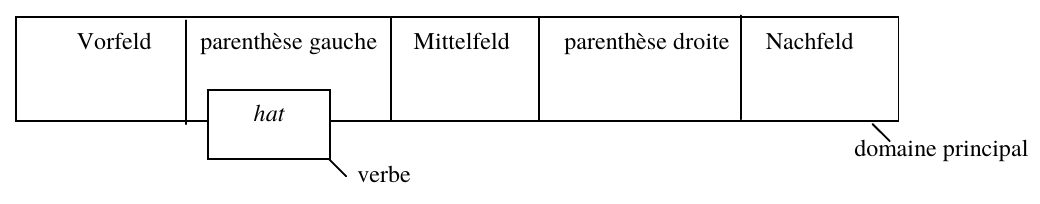
\includegraphics[width=\textwidth]{figures/vol1syntaxe2-img032.png}

    Le verbe principal, c’est-à-dire le verbe qui porte le mode indicatif, comme l’auxiliaire \textit{hat} ‘a’ dans notre exemple, se place en 2\textsuperscript{e} position, appelée \textbf{parenthèse gauche}, après l’unique constituant occupant le \textbf{champ initial} ou \textbf{Vorfeld} ‘pré-champ’. La parenthèse gauche entoure, avec la \textbf{parenthèse droite}, le \textbf{champ du milieu} ou \textbf{Mittelfeld}. Un \textbf{champ final} ou \textbf{Nachfeld} suit la parenthèse droite. Les \textbf{champs} dits \textbf{majeurs} \-– Vorfeld, Mittelfeld et Nachfeld – accueillent les syntagmes nominaux ou adverbiaux. Les dépendants verbaux vont généralement dans la parenthèse droite. Si une phrase n’utilise que le domaine principal pour placer les mots, on parle d’une \textit{structure plate}, par exemple :
    \ea
    \gll Leider hat Peter mal wieder in seiner Nase zu popeln gewagt   vor der ganzen Familie.\\
    Hélas   a   Peter   à nouveau   dans son nez   de creuser osé   devant toute la famille\\
    ‘Peter a malheureusement à nouveau osé se crotter le nez devant toute la famille.’
    \z
    Les parenthèses sont grisées ici. Le constituant \textit{vor der ganzen Familie} ‘devant toute la famille’ peut aller dans le Nachfeld car il est assez lourd (et un placement dans le Mittelfeld séparerait trop les deux parenthèses). Des constituants légers comme \textit{leider} ou \textit{Peter} préfèrent rester dans le Vorfeld ou le Mittelfeld.

    Les propositions subordonnées, complétives et relatives, ont une structure réduite, sans Vorfeld, et l’élément qui introduit la proposition, le complémenteur ou le pronom relatif, occupe la parenthèse gauche. Tous les verbes se placent dans la parenthèse droite. Les verbes recteurs se placent à droite de leur dépendant verbal.

    \ea
    \gll  Ich glaube,   [dass Peter mal wieder in seiner Nase zu popeln\textsubscript{3} gewagt\textsubscript{2} hat\textsubscript{1}   ].\\
    Je crois   [ que  Peter à nouveau dans son nez   de creuser  osé        a   ]\\
    ‘Je crois que Peter a osé se crotter le nez à nouveau.’
    \z
    Le placement des verbes dans la parenthèse droite peut aussi être décrit par une structure topologique : l’amas verbal. Il est composé de trois champs : le \textbf{champ supérieur} ou \textbf{Oberfeld}, le champ tête et le \textbf{champ inférieur} ou \textbf{Unterfeld}.


    \ea
    %%[Warning: Draw object ignored]
    %%[Warning: Draw object ignored]
    %%[Warning: Draw object ignored]
    Oberfeld          champ tête            Unterfeld
    \z
    Sans rentrer dans tous les détails de l’amas verbal, remarquons que pour les dépendants de certains verbes, en particulier les modaux, l’Unterfeld est préférable à l’Oberfeld :

    \ea\label{ex:popel}
    \ea[\textsuperscript{?}]{
    \gll Ich glaube,  [ dass Peter mal wieder in seiner Nase popeln\textsubscript{3} gekonnt\textsubscript{2}  hat\textsubscript{1}   ].\\
        Je crois  [ que   Peter à nouveau dans son nez   creuser  pu           a   ]\\}
    \ex[]{
    \gll Ich glaube,  [ dass Peter mal wieder in seiner Nase hat\textsubscript{1} popeln\textsubscript{3} können\textsubscript{2}   ].\\
    Je crois   [ que   Peter à nouveau dans son nez  a     creuser  pu   ]\\}
    \glt  ‘Je crois que Peter a pu se crotter le nez à nouveau.’
    \z
    \z

    Dans l’exemple a, on observe l’ordre standard dans la parenthèse droite : l’infinitif \textit{popeln} ‘creuser’ se place dans l’Oberfeld du participe \textit{gekonnt} ‘pu’, lui-même placé dans l’Oberfeld de l’auxiliaire \textit{hat} ‘a’. On préfère en fait b, où un «~ersatz~» d’infinitif (all. \textit{Ersatzinfinitiv}), \textit{können} ‘pouvoir’, est réalisé au lieu du participe et où celui-ci est placé dans l’Unterfeld de l’auxiliaire, tandis que \textit{popeln} ‘creuser’ se place à nouveau dans l’Oberfeld de son gouverneur. Cette construction est appelée l’\textit{Oberfeldumstellung} ‘conversion du champ supérieur’. Pour certains locuteurs de l’allemand, le verbe \textit{popeln} peut se placer dans l’Oberfeld de l’auxiliaire, non occupé par le dépendant direct de l’auxiliare. Cette nouvelle construction est appelée le \textit{Zwischenstellung} ‘position intermédiaire’ avec l’auxilaire entre les deux verbes à l’infinitif :

    \begin{exe}
    \exr{ex:popel}
    \begin{xlist}
    \exi[c.] \textit{Ich glaube,}  [ \textit{dass Peter mal wieder in seiner Nase}  \textit{popeln\textsubscript{3}} \textit{hat\textsubscript{1} }\textit{können\textsubscript{2}}   ].\textit{\\
    }  Je crois   [ que   Peter à nouveau dans son nez  creuser  a     pu   ]\\
    ‘Je crois que Peter a pu se crotter le nez à nouveau.’
    \end{xlist}
    \end{exe}
}
\loupe{L’anglais comme langue de référence}{%\label{sec:3.5.37}
    Peu d’approches théoriques distinguent, comme nous le faisons, la structure syntaxique de la structure topologique. Nous pensons que la non-prise en compte de la topologie doit beaucoup au fait que l’anglais sert de langue de communication dans le monde scientifique et donc de langue de référence de très nombreux travaux en linguistique. Or l’anglais est, du point de vue typologique (c’est-à-dire lorsqu’on prend en compte la diversité des langues), une langue particulièrement «~exotique~». En effet, l’anglais a un ordre des syntaxèmes singulièrement rigide, avec non seulement une position fixe du sujet devant le verbe, mais aussi l’obligation de placer l’objet direct avant les autres compléments. Cette particularité permet de postuler une sorte de groupe verbal (voir l’\encadref{fig:3.4.20} sur \textit{Le groupe verbal}) au niveau topologique en anglais. Par ailleurs, le fait que la structure syntaxique et la structure topologique soit si fortement liée peut amener à les identifier et donc à considérer aussi un constituant syntaxique VP au niveau syntaxique, comme le font les générativistes.

    Cela va plus loin encore, car les mêmes générativistes considèrent que toutes les langues devraient avoir un VP. Les langues qui autorisent le placement du sujet entre le V et l’objet, contredisant de fait l’existence d’un VP, sont alors dites \textbf{non-configurationnelles}. Certains linguistiques, dont Chomsky, considèrent qu’il y a bien un VP sous-jacent, mais que les syntaxèmes sont systématiquement déplacés en surface (voir l’\encadref{fig:3.2.6} sur \textit{Linéarisation et mouvement}). C’est une analyse que nous rejetons totalement.
}
\chevalier{Historique de la description topologique}{%\label{sec:3.5.38}
    Nous avons déjà mentionné à deux reprises la contribution de Gabriel \citet{Girard1747} à la modélisation de l’ordre des mots. Son ouvrage contient une dizaine de \textbf{règles de précédence linéaire~}remarquablement formalisées. Par exemple :

    \begin{quote}
    «~Première Règle. – Dans la forme expositive, le Subjectif marche ordinairement devant l’Attributif : celui-ci y précède à son tour l’Objectif et le Terminatif, lorsqu’ils sont énoncés par des expressions formelles et non simplement désignés par des pronoms personnels ou relatifs.~»
    \end{quote}

    Cette règle indique que, dans la phrase déclarative, le sujet (= Subjectif) se place devant le prédicat verbal (= Attributif), qui lui-même précède l’objet direct (= Objectif) et l’objet indirect (= Terminatif), à moins que ceux-ci ne soient des pronoms personnels ou relatif. Les règles suivantes indiquent que le sujet se place après le verbe dans les propositions en incise (Règle II), que le sujet peut se placer après le verbe en l’absence d’un objet direct ou quand celui-ci est un pronom (Règle III), etc.

    Le modèle topologique, avec ses gabarits de places fixes, s’est développé au siècle suivant en Allemagne. Simon (Heinrich Adolf) \citet{Herling1821} propose la première théorie globale sur la structure hiérarchique des phrases complexes de l’allemand basée sur des gabarits de places fixes. Oskar \citet{Erdmann1886} poursuit le travail de Herling en énumérant le type d’éléments que ces places peuvent contenir, donnant ce que \citet{Höhle1986} propose d’appeler le système de Herling-Erdmann et qu’on appelle plus souvent aujourd’hui la théorie des champs topologiques. Le terme \textit{Feld} ‘champ’ pour désigner ces places dans la phrase apparaît pour la première fois chez Erich \citet{Drach1937} dans un livre intitulé~\textit{Grundgedanken der Deutschen Satzlehre} ‘Idées fondamentales de la phrase allemande’ destiné aux enseignants de l’allemand comme langue maternelle et langue étrangère. Le livre de Drach prône, avec une teinte légèrement nationalisante, une émancipation de la grammaire allemande, qui était jusqu’à là sous une influence latine forte, en faveur d’une «~construction d’une présentation et d’un système de règles basé sur la nature de la langue allemande~». Gunnar \citet{Bech1955} a adapté par la suite la terminologie de Drach pour décrire la structure interne du complexe verbal.

    Le modèle topologique a été appliqué par Povl Skårup \REF{ex:key:1975} à la description de l’ordre des mots en ancien français, montrant l’influence des langues germaniques sur l’émergence du français. Gerdes et \citet{Kahane2006} proposent le modèle topologique pour le français présenté dans ce chapitre, qui s’appuie notamment sur les travaux sur la macrosyntaxe de Claire Blanche-\citet{Benveniste1990}. Le modèle topologique a aussi été appliqué à des langues clairement non germaniques, comme dans la description par \citet{DonohueSag1999} du warlpiri, une langue aborigène d’Australie à ordre très libre.

    La question de l’ordre des mots a été peu traitée dans les premières grammaires formelles. Dans les grammaires de constituants, l’ordre linéaire est intégré à la structure syntaxique et toute variation de l’ordre des mots suppose un changement de structure syntaxique (voir l’\encadref{fig:3.2.7} \textit{De la non-séparation des ordres au mouvement}). Il faudra attendre le début des années 1980 pour que soient proposées des grammaires de constituants où les \textbf{règles de précédence linéaire} sont séparées des règles de sous-catégorisation, notamment avec le modèle GPSG \citep{GazdarEtAl1985}, qui donnera ensuite HSPG (\citealt{PollardSag1987}). Le modèle topologique de l’allemand sera formalisé pour la première fois par Andreas \citet{Kathol1995} dans le cadre de HPSG.

    Dans le cadre des grammaires de dépendance, Igor Mel’čuk et Nicolaj \citet{Pertsov1987} proposent une liste très complète des constructions de l’anglais et des règles de précédence linéaire qui vont avec. Le modèle topologique sera formalisé en grammaire de dépendance simultanément par Duchier et \citet{Debusmann2001} et Gerdes et \citet{Kahane2001} (voir la formalisation proposée dans l’\encadref{fig:3.5.33} \textit{Grammaire topologique formelle}).
}
\exercices{%\label{sec:3.5.39}
    \exercice{1} a) Qu’est-ce que la topologie ?

    b) À quel endroit du modèle linguistique le modèle topologique intervient-il dans un modèle stratificationnel comme la théorie Sens-Texte (voir \sectref{sec:1.3.8} \textit{Modularité et stratification} et \encadref{fig:1.3.9} \textit{La Théorie Sens-Texte}) ?

    c) Pourquoi rejetons-nous la notion d’ordre de base ?

    \exercice{2} Ordre préfixé et postfixé. a) On considère l’expression préfixée × 3 + × 12 5 7. Donner l’arbre de dépendance correspondant et en déduire une expression infixée et postfixée.

    b) On considère l’expression postfixée 1 5 ${\surd}$ + 2 /. Sachant que ${\surd}$ (racine carrée) est un opérateur unaire (c’est-à-dire d’arité 1), donner l’arbre de dépendance correspondant à cette expression. En déduire l’écriture traditionnelle de ce nombre (qui n’est autre que le nombre d’or).

    \exercice{3} Projectivité. Construire la structure de dépendance de la phrase suivante et vérifier qu’elle est non projective :

    À \textit{cette heure-là, je pense qu’il est déjà parti.}

    \exercice{4} Théorie des graphes. Le graphe K\textsubscript{4} n’est pas planaire extérieur (voir \encadref{fig:3.5.15} \textit{Projectivité et planarité}). Montrer qu’il est néanmoins planaire et que donc tous les graphes de 4 nœuds ou moins sont planaires. Chercher les graphes non-planaires les plus simples à 5 et à 6 nœuds.

    \exercice{5} Topologie du groupe substantival en français. On s’intéresse plus particulièrement au placement des déterminants et des numéraux en français. Comment rendre compte des données suivantes dans un modèle topologique ?

    \ea
    {les/mes/ces/deux/quelques/des/plusieurs amis sont venus}
    \z
    \ea
    {les/mes/ces deux/quelques amis sont venus}
    \z
    \ea
    {*les mes/ces/des/plusieurs amis sont venus}
    \z
\ea{
    *amis sont venus
    }
    \z

    \exercice{6} Interrogation en français. On observe un contraste entre le fonctionnement des interrogatifs \textit{à qui} et \textit{que~}:
    \ea
    {À qui parle-t-elle} ?
    \z
\ea{
    À qui Marie parle-t-elle ?
    }
    \z
\ea{
    Que dit-elle ?
    }
    \z
\ea{
    *Que Marie dit-elle ?
    }
    \z
    Comment expliquer cette différence de comportement dans le cadre d’un modèle topologique ?

    \exercice{7} Topologie de l’anglais. L’anglais possède une classe de verbes que l’on appelle les modaux qui comprend les auxiliaires \textsc{be} ‘être’ et \textsc{have} ‘avoir’ et quelques verbes à valeur modale comme \textsc{can} ‘pouvoir, \textsc{must} ‘devoir, \textsc{will} (auxiliaire du futur) ou \textsc{would} (auxiliaire du conditionnel) qui ont la particularité d’être invariables, ainsi que \textsc{do} ‘faire’. Ces verbes ont également des propriétés distributionnelles qui les distinguent des autres verbes. Premièrement, les adverbes se placent de préférence après les modaux et avant les verbes ordinaires :
    \ea
    {Mary often calls Peter}     ‘Marie appelle souvent Pierre’
    \z
    \ea
    {\textsuperscript{??}}\textit{Mary calls often Peter}
    \z
    \ea
    {Mary would often call Peter}   ‘Marie appellerait souvent Pierre’
    \z
    \ea
    {\textsuperscript{??}}\textit{Mary often would call Peter}
    \z

    Deuxièmement, dans les interrogatives, le sujet se place entre le modal et le verbe, et en cas d’absence de modal, \textsc{do} est introduit :
    \ea
    {Would Mary call Peter?}     ‘Marie appellerait-elle Pierre ?’
    \z
    \ea
    {*Calls Mary Peter?}
    \z
    \ea
    {Does Mary call Peter?}     ‘Marie appelle-t-elle Pierre ?’
    \z
    La position initiale peut aussi être occupée par un pronom interrogatif :
    \ea
    {Why would Mary call Peter?}   ‘Pourquoi Marie appellerait-elle Pierre ?’
    \z
    \ea
    {Who does Mary call?}     ‘Qui Marie appelle-t-elle ?’
    \z
    Troisièmement, la négation se place obligatoirement sur un modal et donc comme dans le cas de l’interrogation, \textsc{do} doit être introduit en l’absence d’un autre modal :
    \ea
    {Mary would not call Peter}     ‘Marie n’appellerait pas Pierre’
    \z
\ea{
    *Mary calls not Peter
    }
    \z
    \ea
    {Mary does not call Peter}    ‘Marie n’appelle pas Pierre’
    \z

    Quatrièmement, le sujet peut être inversé dans certains cas :
    \ea
    {Never would Mary call Peter}   ‘Jamais Marie n’appellerait Pierre’
    \z
    \ea
    {Here are two nice people}     ‘Ici sont deux chouettes personnes’
    \z
    Rappelons également que, en anglais, l’objet direct doit précéder tous les autres compléments. De quelle façon un modèle topologique de l’anglais peut-il rendre compte de ces propriétés ?

    \exercice{8} Topologie de l’allemand. Les exemples que nous avons présentés dans l’\encadref{fig:3.5.36} acceptent encore d’autres ordres, comme, par exemple :

    \ea
    \gll In seiner Nase zu popelnhatPetermal wieder gewagt.\\
    dans son nez  de creuser  a   Peter   à nouveau   osé\\
    \glt   ‘Peter a à nouveau osé se crotter le nez.’
    \z

    Comment pouvez-vous intégrer cet exemple au modèle topologique de l’allemand ?

    \exercice{9} Ce que nous avons fait pour le français, l’allemand, le russe ou l’anglais peut être fait pour n’importe quelle langue a priori. Nous avons déjà écrit des modèles topologiques pour l’arabe, le chinois ou le wolof. Vous pouvez essayer d’écrire un fragment de modèle topologique pour la langue de votre choix et nous l’envoyer.
}
\lecturesadditionnelles{% \label{sec:3.5.40}
    Comme nous l’avons déjà mentionné au \chapref{sec:3.3}, on peut consulter en ligner la plupart des ouvrages anciens. On trouvera facilement \citet{Buffier1709}, \citet{Girard1747}, \citet{Weil1844}, ainsi que les articles de Beauzée et Dumarsais dans l’\textit{Encyclopédie} de Diderot et D’Alembert (voir \chapref{sec:3.3}).

    Les premiers travaux sur le modèle topologique sont en allemand : \citet{Erdman1886}, \citet{Drach1937}, \citet{Bech1955}. Pour des travaux plus récents sur l’ordre des mots, nous avons mentionné \citet{GazdarEtAl1985}, \citet{PollardSag1994}, Mel’čuk \& \citet{Pertsov1987}, \citet{Kathol1995} ainsi que les articles de \citet{BresnanEtAl2007}, \citet{DuchierDebusmann2001} et \citet{GerdesKahane2001,GerdesKahane2006}. Sur la structure communicative et son rôle dans l’ordre des mots, nous renvoyons à \citet{Lambrecht1996} et Mel’čuk \REF{ex:key:2001}.

    Pour les travaux typologiques sur l’ordre des mots, on consultera l’article original de \citet{Greenberg1963} et l’étude et le travail très complet de \citet{Dryer1992}, ainsi que les cartes et les différents articles consacrés à l’ordre des mots sur le site wals.info, une base de données typologique où sont répertoriés 192 traits pour plus de 2500 langues !

    Joan Bresnan, Anna Cueni, Tatiana Nikitina, R. Harald \citet{Baayen2007}. Predicting the dative alternation, \textit{Cognitive foundations of interpretation}, KNAW, 69-94.

    Gunnar \citet{Bech1955} \textit{Studien über das deutsche Verbum infinitum} [Étude sur le verbe infinitif allemand], Band I (= Det Kongelige Danske Videnskabernes Selskab, Historisk-filosofiske Meddelelser 35, no. 2), Copenhague.

    Erich \citet{Drach1937} \textit{Grundgedanken der deutschen Satzlehre} [Idées fondamentales de la syntaxe allemande] Diesterweg, Frankfurt am Main.

    Matthew S. \citet{Dryer1992} \textstylest{The} Greenbergian Word Order Correlations\textstylest{, \textit{Language}, 68(1), 81-138.}

    Denys Duchier, Ralph \citet{Debusmann2001} Topological dependency trees: A constraint-based account of linear precedence, \textit{Proceedings of the 39th Annual Meeting of the Association for Computational Linguistics} (\textit{ACL}).

    Oskar \citet{Erdmann1886} \textit{Grundzüge der deutschen Syntax nach ihrer geschichtlichen Entwicklung} [Caractéristiques de base de la syntaxe allemande selon son évolution historique], Vol. 1. JG Cotta.

    Gerald Gazdar, Ewan Klein, Geoffrey Pullum, Ivan \citet{Sag1985} \textit{Generalized phrase structure grammar}. Harvard University Press.

    Simon Heinrich Adolf \citet{Herling1821} \textit{Uber die Topik der deutschen Sprache,} Varrentrapp.

    Kim Gerdes, Sylvain \citet{Kahane2001} Word order in German: A formal dependency grammar using a topological hierarchy, \textit{Proceedings of the 39th Annual Meeting of the Association for Computational Linguistics} (\textit{ACL}).

    Kim Gerdes, Sylvain \citet{Kahane2006} L’amas verbal au cœur d’une modélisation topologique du français, \textit{Lingvisticae Investigationes}, 29(1), 75-89.

    Joseph H. \citet{Greenberg1963} Some universals of grammar with particular reference to the order of meaningful elements, in J. H. Greenberg, \textit{Universals of language}, 73-113.

    Andreas \citet{Kathol1995} \textit{Linearization-based German syntax}, thèse de doctorat, The Ohio State University.

    Knud \citet{Lambrecht1996} \textit{Information structure and sentence form: Topic, focus, and the mental representations of discourse referents}. Vol. 71. Cambridge University Press.

    Igor Mel’čuk, Nicolaj \citet{Pertsov1987} \textit{Surface Syntax of English: A Formal Model within the Meaning-Text Framework}, Benjamins.

    Igor Mel’čuk \REF{ex:key:2001} \textit{Communicative organization in natural language}, Benjamins.

    Carl Pollard, Ivan A. \citet{Sag1994} \textit{Head-driven phrase structure grammar}, University of Chicago Press.

    Povl Skårup \REF{ex:key:1975} \textit{Les premières zones de la proposition en ancien français: essai de syntaxe de position}. Vol. 6., Akademisk Forlag.
}
\corrections{%\label{sec:3.5.41}
    \corrigé{1}
    a) La topologie est l’étude du placement des unités syntaxiques, c’est-à-dire l’étude de l’ordre des mots, mais aussi des syntaxèmes à l’intérieur des mots.

    b) Le modèle linguistique décrit la correspondance entre le sens et le texte. Le modèle topologique décrit la linéarisation, c’est-à-dire la correspondance entre la structure syntaxique (non ordonnée) et la chaîne linéaire. Ou dans sa version plus élaborée entre une structure de dépendance syntaxique et un arbre de constituants topologiques.

    c) Certaines langues ont un ordre dominant, comme l’ordre SVO en français. Néanmoins considérer un ordre de base revient à considérer que tous les autres ordres sont obtenus par des transformations de l’ordre base. Cela revient à dire que lorsque le sujet est après le verbe en français, celui-ci a été inversé. Même s’il peut nous arriver de conserver la terminologie et de parler de «~sujet inversé~», nous ne considérons pas qu’il y a eu une inversion. Nous considérons que le sujet a été placé directement dans cette position.

    \corrigé{2} 1) Le premier symbole, ×, est la racine de l’arbre. Son premier dépendant est 3. Le symbole suivant, +, est la racine du deuxième dépendant, et ainsi de suite. La formule est donc 3 × ((12×5) + 7) sous forme infixée et 3 12 5 × 7 + × sous forme postfixée.

    2) La formule est (1 + ${\surd}$5) / 2 sous forme infixée et / + 1 ${\surd}$ 5 2 sous forme préfixée.

    \corrigé{3} Le syntagme \textit{à cette heure-là} dépend de \textit{parti} et couvre donc la racine de l’arbre \textit{pense}.

    \corrigé{4} Le graphe K\textsubscript{4} est planaire : il suffit de prendre une des diagonales et de la faire passer par l’extérieur du carré. C’est le plus complexe des graphes à 4 nœuds et donc tous les graphes à 4 nœuds ou moins sont planaires. Le plus petit graphe non planaire à 5 nœuds est K\textsubscript{5}, le graphe complet à 5 nœuds. Le plus petit graphe non planaire à 6 nœuds est K\textsubscript{3,3}, le graphe où 3 nœuds sont liés aux 3 autres. On vérifiera que, si on retire un seul de leurs liens, ces graphes deviennent planaires.

    \ea
    %%[Warning: Draw object ignored]
    \z

    Le mathématicien polonais Kazimierz Kuratowski a établi en 1930 la caractérisation suivante des graphes planaires : Un graphe est planaire si et seulement s’il ne peut être réduit ni à K\textsubscript{5}, ni à K\textsubscript{3,3}.

    On pourra consulter les pages de la wikipédia sur les graphes planaires et planaires extérieurs.

    \corrigé{5} On observe trois paradigmes de «~déterminants~» : 1) \textit{les, mes, ces~}; 2) \textit{des, plusieurs~}; 3) \textit{deux, quelques}. Les éléments de types 1 et 3 peuvent cooccurrer, tandis que ceux de types 2 excluent les autres. Les noms communs doivent obligatoirement être accompagnés d’au moins un éléments d’un de ces trois types. Les éléments de type 1 sont les déterminants définis, ceux de type 2 les déterminants indéfinis. Quant à ceux de type 3, ce sont des quasi-déterminants, puisqu’ils peuvent se placer entre un déterminant défini et le nom et qu’ils n’ont pas de valeur intrinsèquement définie ou indéfinie, mais ils prennent une valeur indéfinie en l’absence d’un déterminant défini. On peut modéliser cette distribution en considérant deux champs topologiques : un pour les déterminant définis, suivi d’un pour les quasi-déterminants, avec la condition qu’un des deux champs au moins doit être occupé. Les déterminants indéfinis occuperaient quant à eux occuperaient les deux champs en même temps. (Ou ce qui revient au même, ils occupent le champ des quasi-déterminants, mais excluent, pour des raisons sémantiques, la cooccurrence avec un déterminant défini.)

    \corrigé{6} Les pronoms interrogatifs se placent au début du domaine microsyntaxique, devant le sujet (dans \textit{Marie, à qui parle-t-elle} ?, \textit{Marie} est détaché et l’occupe plus la position sujet). Le pronom interrogatif \textit{que} est la forme faible du pronom \textit{quoi} (comme \textit{me} avec \textit{moi}). C’est un clitique qui doit obligatoirement être dans l’amas verbal (comme \textit{me}). Autrement dit, le pronom niterrogatif \textit{que} doit à la fois être en tête du domaine microsyntaxique et dans l’amas verbal, ce qui écrase tout ce qui se trouve entre les deux et en particulier le champ initial qu’occuperait le sujet.

    \corrigé{7} Les modaux de l’anglais occupent un champ topologique différent de celui des verbes. Le domaine de la phrase déclarative contient les champs suivants :

    ch\_initial {\textbar} ch\_modal {\textbar} ch\_adv {\textbar} ch\_verbal {\textbar} ch\_objet {\textbar} ch\_compl

    Le sujet va dans le champ initial, sauf quand celui-ci est occupé par un pronom interrogatif, une négation ou un locatif, ou quand il reste vide dans une interrogative totale. Le champ modal peut rester vide quand le sujet occupe le champ initial et qu’il n’y a pas la négation \textit{not} dans le champ adverbial. Le sujet inversé va dans le champ adverbial.

    \corrigé{8} Cet exemple montre qu’un constituant à tête verbale, comme \textit{in seiner Nase zu popeln} ‘de se crotter le nez’, peut également venir se placer dans le Vorfeld. Il n’est pas nécessaire d’aménager davantage le modèle.
}
